\documentclass[cjk]{loom-book}
\usepackage{graphicx}
\usepackage{longtable}
\usepackage{newunicodechar}
\usepackage{caption}
\usepackage{eso-pic}
\providecommand{\aj}{AJ}
\providecommand{\actaa}{Acta Astron.}
\providecommand{\araa}{ARA\&A}
\providecommand{\apj}{ApJ}
\providecommand{\aplett}{Astrophys. Lett.}
\providecommand{\apjl}{ApJ}
\providecommand{\apjs}{ApJS}
\providecommand{\ao}{Appl. Opt.}
\providecommand{\apss}{Ap\&SS}
\providecommand{\aap}{A\&A}
\providecommand{\aapr}{A\&A Rev.}
\providecommand{\aaps}{A\&AS}
\providecommand{\azh}{AZh}
\providecommand{\baas}{BAAS}
\providecommand{\caa}{Chinese Astron. Astrophys.}
\providecommand{\cjaa}{Chinese J. Astron. Astrophys.}
\providecommand{\icarus}{Icarus}
\providecommand{\jcap}{JCAP}
\providecommand{\jcp}{J. Chem. Phys.}
\providecommand{\jrasc}{JRASC}
\providecommand{\memras}{MmRAS}
\providecommand{\mnras}{MNRAS}
\providecommand{\na}{New Astron.}
\providecommand{\nar}{New Astron. Rev.}
\providecommand{\pra}{Phys. Rev. A}
\providecommand{\prb}{Phys. Rev. B}
\providecommand{\prc}{Phys. Rev. C}
\providecommand{\prd}{Phys. Rev. D}
\providecommand{\pre}{Phys. Rev. E}
\providecommand{\prl}{Phys. Rev. Lett.}
\providecommand{\pasa}{PASA}
\providecommand{\pasp}{PASP}
\providecommand{\pasj}{PASJ}
\providecommand{\physrep}{Phys. Rep.}
\providecommand{\qjras}{QJRAS}
\providecommand{\rmxaa}{Rev. Mexicana Astron. Astrofis.}
\providecommand{\skytel}{Sky Telesc.}
\providecommand{\solphys}{Sol. Phys.}
\providecommand{\sovast}{Soviet Ast.}
\providecommand{\ssr}{Space Sci. Rev.}
\providecommand{\zap}{ZAp}
\providecommand{\nat}{Nature}
\providecommand{\sci}{Science}
\providecommand{\grl}{Geophys. Res. Lett.}
\providecommand{\textdegree}{\ensuremath{^\circ}}
\makeatletter
\@ifundefined{textregistered}
  {\newcommand{\textregistered}{\ifmmode\scriptscriptstyle\circledR\else\textsuperscript{\textcircled{\scriptsize R}}\fi}}
  {\renewcommand{\textregistered}{\ifmmode\scriptscriptstyle\circledR\else\textsuperscript{\textcircled{\scriptsize R}}\fi}}
\makeatother

\newcommand{\bm}[1]{\symbf{#1}}

\runningthread{量子天文学}

\hypersetup{
  colorlinks=true,
  linkcolor=indigo,
  citecolor=madder,
  urlcolor=indigo
}

\captionsetup{
  font={small,sf},
  labelfont={bf,color=indigo},
  textfont={color=inkiron!90!white},
  labelsep=quad,
  skip=5pt
}

\renewcommand{\contentsname}{目录}
\renewcommand{\bibname}{参考文献}
\renewcommand{\figurename}{图}
\renewcommand{\tablename}{表}
\renewcommand{\partname}{部分}
\renewcommand{\figureautorefname}{图}
\renewcommand{\tableautorefname}{表}
\renewcommand{\equationautorefname}{式}
\renewcommand{\sectionautorefname}{节}
\renewcommand{\subsectionautorefname}{节}

\newcommand{\citationneeded}{\textsuperscript{[citation needed]}}
\newunicodechar{─}{--}
\newenvironment{chapteropening}{\begin{strand}}{\end{strand}}
\setlength{\emergencystretch}{3em}
\tolerance=2000
\allowdisplaybreaks[1]

\begin{document}
\frontmatter
\newcommand{\bookauthorname}{Yu Wang}
\newcommand{\bookauthoremail}{yu.wang@icranet.org}
\newcommand{\bookaffiliationA}{ICRA, Dipartimento di Fisica, Sapienza Universit\`a di Roma, Piazzale Aldo Moro 5, I-00185 Roma, Italy}
\newcommand{\bookaffiliationB}{ICRANet, Piazza della Repubblica 10, I-65122 Pescara, Italy}
\newcommand{\bookaffiliationC}{INAF--Osservatorio Astronomico d'Abruzzo, Via M. Maggini snc, I-64100 Teramo, Italy}
\newcommand{\bookaffiliationD}{Marcel Grossmann Center, Brickell Avenue 701, Miami, FL 33131, USA}

\newcommand{\bookauthorblock}{%
  \bookauthorname\\
  \href{mailto:\bookauthoremail}{\texttt{\bookauthoremail}}\\[0.6em]
  \begin{minipage}{0.86\textwidth}
    \centering\small
    \bookaffiliationA\\
    \bookaffiliationB\\
    \bookaffiliationC\\
    \bookaffiliationD
  \end{minipage}%
}

\newcommand{\bookcoverimage}{figures/generated/cover-cn.png}
\newcommand{\makebookimagecover}{%
  \hypersetup{pageanchor=false}%
  \thispagestyle{empty}%
  \AddToShipoutPictureBG*{%
    \AtPageLowerLeft{%
      \includegraphics[width=\paperwidth,height=\paperheight]{\bookcoverimage}%
    }%
  }%
  \mbox{}%
  \clearpage
  \hypersetup{pageanchor=true}%
}

\newcommand{\makebooktitlepage}[3]{%
  \thispagestyle{empty}%
  \vspace*{0.34\textheight}
  \begin{center}
    {\Large #1\par}
    \vspace{2.2em}
    {#2\par}
    \vspace{2em}
    {#3\par}
  \end{center}
  \clearpage
}

\makebookimagecover

\makebooktitlepage{量子天文学}{\bookauthorblock}{第一版工作稿，2026-07-01}
\weave

{\small\tableofcontents}

\chapter*{前言}
\addcontentsline{toc}{chapter}{前言}

写这本书的原因，是我想要学习量子天文学。

我最初想找一本从观测出发的教材，从真实的天文数据讲起，再逐步引入相干函
数、光子统计、量子估计和仪器限制等等。我没有找到这样一本书。相关内容当然存在，
许多论文和专著也写得很好，但它们分散在统计光学、量子光学、干涉测量、高能天体物理、宇
宙学和量子信息里。

于是我决定自己写一本，也把写作当成学习的一部分。这本书仍然在更新，因为我仍然在学习。

\begin{flushright}
王瑜\\
2026 年 7 月
\end{flushright}


\mainmatter
\part[基础、定义和观测量]{基础、定义和观测量}
\chapter{最基础的概念}
\label{chap:01}

\begin{chapteropening}
望远镜收到的“光”在数据里到底变成了什么？一台望远镜不会直接保存一束连续电磁波，也不会直接保存一张已经有物理解释的图像。它最终保存的是计数、时间、通道、位置和质量标记。

最基础的语言从这里开始：光可以用电场描述；探测器通常只留下强度和光子计数；事件表、Poisson 噪声和几个数量级共同决定公式里的基本单位和基本数据字段。
\end{chapteropening}

\section{望远镜真正记录了什么}
\label{sec:1-language}

最底层的数据不是“图像”，而是一条条事件。一次光子探测可以记为
\begin{equation}
  e_j=(t_j,\bm{r}_j,\nu_j,p_j,w_j).
  \label{eq:event-row}
\end{equation}
\begin{formulaexplain}
\(e_j\) 表示第 \(j\) 条探测事件；\(t_j\) 是时间戳，\(\bm r_j\) 是接收位置或像素，\(\nu_j\) 是频率通道，\(p_j\) 是偏振或电子学通道，\(w_j\) 是质量权重。这条式子的意义是把一次光子点击写成可分析的数据行。
\end{formulaexplain}
这里 \(j\) 是事件编号；\(t_j\) 是到达时间，单位通常是秒、纳秒或皮秒；\(\bm r_j\) 表示接收位置，可以是望远镜编号、探测器像素或阵列坐标；\(\nu_j\) 是频率或光谱通道，单位 Hz 或通道号；\(p_j\) 是偏振、探测器或电子学通道标签；\(w_j\) 是权重或质量标记，可以记录背景概率、坏像素、死时间附近事件、云层筛选或效率修正。

这行式子不是为了复杂化数据，而是为了提醒我们：同一批光子可以被投影成很多不同产品。若按天空位置分箱，就得到图像；按频率分箱，就得到光谱；按时间分箱，就得到光变曲线；按偏振通道组合，就得到偏振量。每一次投影都会保留一部分信息，也会丢掉一部分信息。后面的章节之所以反复回到事件表，是因为许多快速变化、通道相关和时间相关问题一旦先被平均，就很难再恢复。

\section{光为什么既有波的语言也有计数的语言}
\label{sec:1-light}

在一个足够窄的频率通道里，光可以先近似看成单色电磁波。真实振荡的是电场，例如
\begin{equation}
  E(t)=E_0\cos(\omega t+\phi),
  \qquad \omega=2\pi\nu .
  \label{eq:monochromatic-field}
\end{equation}
\begin{formulaexplain}
\(E(t)\) 是时刻 \(t\) 的真实电场；\(E_0\) 是振幅；\(\omega\) 是角频率；\(\nu\) 是普通频率；\(\phi\) 是相位。它说明单色光的波动信息首先存在于电场的快速振荡中。
\end{formulaexplain}
\(E_0\) 是电场振幅，\(\omega\) 是角频率，\(\nu\) 是频率，\(\phi\) 是相位。可见光频率约为 \(4\times10^{14}\) 到 \(8\times10^{14}\,{\rm Hz}\)，一个光学周期只有几飞秒。普通天文探测器的响应远慢于这个周期，因此它通常不会逐周期记录 \(E(t)\) 的正负振荡。

为了同时表示振幅和相位，常把电场写成复振幅：
\begin{equation}
  \mathcal{E}=E_0e^{i\phi},
  \qquad
  E(t)=\operatorname{Re}\!\left[\mathcal{E}e^{i\omega t}\right].
  \label{eq:phasor-field}
\end{equation}
\begin{formulaexplain}
\(\mathcal E\) 是复振幅；\(|\mathcal E|=E_0\) 给出振幅；\(\arg\mathcal E=\phi\) 给出相位；\(\operatorname{Re}\) 表示取实部。这条式子把振幅和相位合进一个复数，方便讨论干涉。
\end{formulaexplain}
\(\mathcal E\) 的模 \(|\mathcal E|=E_0\) 表示振幅，辐角 \(\arg\mathcal E=\phi\) 表示相位。可以把它想成一支旋转箭头：长度是振幅，方向是相位。相位的单位是弧度，本质上是无量纲角变量。

探测器真正留下的通常是强度或光子数。把光学快速振荡在探测器响应时间内平均后，强度近似正比于电场平方：
\begin{equation}
  I\propto \langle E^2(t)\rangle_{\rm det}
  \propto |\mathcal{E}|^2 .
  \label{eq:intensity-from-field}
\end{equation}
\begin{formulaexplain}
\(I\) 是探测到的强度；\(\langle\cdots\rangle_{\rm det}\) 表示在探测器响应时间内平均；\(|\mathcal E|^2\) 是复振幅模平方。它说明探测器通常记录能量相关量，而不是电场的瞬时正负振荡。
\end{formulaexplain}
物理上，这条式子说的是：探测器吸收能量，能量密度和场的平方有关。因此相位本身通常不会被直接记录；它只能通过干涉、调制或后续的相关测量间接影响强度数据。

最简单的干涉来自两束光的电场相加。若两束光进入同一探测器，先相加的是电场，后平方的是强度：
\begin{equation}
  I\propto |\mathcal{E}_1+\mathcal{E}_2|^2
  =
  |\mathcal{E}_1|^2+|\mathcal{E}_2|^2
  +2\,\operatorname{Re}(\mathcal{E}_1\mathcal{E}_2^\ast).
  \label{eq:two-beam-interference}
\end{equation}
\begin{formulaexplain}
\(\mathcal E_1,\mathcal E_2\) 是两束光的复振幅；前两项是各自强度；\(2\operatorname{Re}(\mathcal E_1\mathcal E_2^\ast)\) 是交叉干涉项；星号表示复共轭。这条式子说明普通干涉来自电场先相加再取模平方。
\end{formulaexplain}
前两项是两束光各自的强度；最后一项是干涉项。如果写成 \(\mathcal E_1=E_1e^{i\phi_1}\)、\(\mathcal E_2=E_2e^{i\phi_2}\)，干涉项就是 \(2E_1E_2\cos(\phi_1-\phi_2)\)。相位差接近 0 时相长，接近 \(\pi\) 时相消。后面的干涉测量章节会在这个基本事实上继续展开。

天文学里最常见的几何相位来自路程差：
\begin{equation}
  \Delta\phi=\frac{2\pi}{\lambda}\,\bm B\cdot\bm s .
  \label{eq:geometric-phase}
\end{equation}
\begin{formulaexplain}
\(\Delta\phi\) 是几何相位差；\(\lambda\) 是波长；\(\bm B\) 是两接收点的基线；\(\bm s\) 是源方向单位向量；\(\bm B\cdot\bm s\) 是路程差。这条式子把望远镜几何换成光学相位。
\end{formulaexplain}
\(\bm B\) 是两处接收点之间的基线向量，单位厘米；\(\bm s\) 是源方向单位向量；\(\lambda\) 是波长。点积 \(\bm B\cdot\bm s\) 是沿源方向的路程差，\(2\pi/\lambda\) 把长度换成相位。多走一个波长，相位就多 \(2\pi\)。这条式子只给出最基础的相位语言；两台望远镜之间更完整的空间关系将在第 \ref{chap:05} 章正式定义。

\begin{figure}[tbp]
\centering
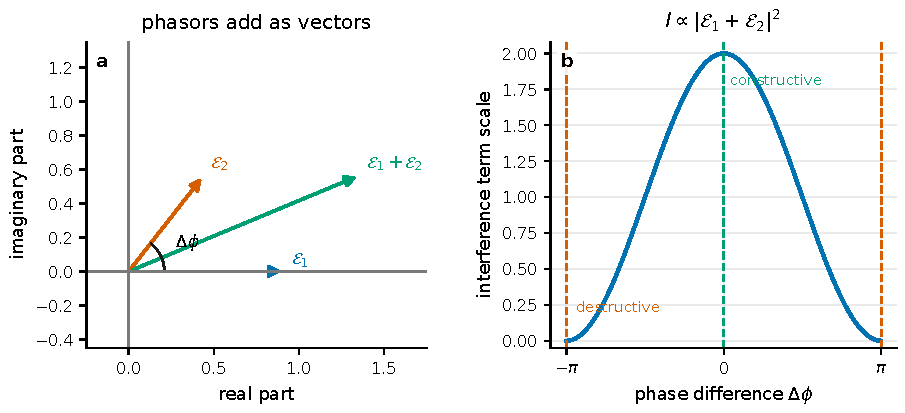
\includegraphics[width=0.86\linewidth]{figures/generated/chapter_01/ch01_phase_interference.pdf}
\caption{复振幅和两束光干涉的基本图像。复振幅像箭头一样相加；探测器看到的是合成箭头长度的平方。相位差决定干涉项是正、负还是被平均掉。}
\label{fig:ch01-phase-interference}
\end{figure}

\section{为什么计数会有噪声}
\label{sec:1-counting}

探测器把光变成离散点击以后，最基本的随机量就是某个时间窗内的计数。选定时间 bin 宽度 \(\Delta t\)，若平均光子到达率为 \(R_\gamma\)，则平均计数为
\begin{equation}
  \mu=R_\gamma\Delta t .
  \label{eq:mean-count}
\end{equation}
\begin{formulaexplain}
\(\mu\) 是一个时间 bin 中的平均光子数；\(R_\gamma\) 是平均光子到达率；\(\Delta t\) 是时间 bin 宽度。它把连续的光子率换成离散计数模型中的平均数。
\end{formulaexplain}
\(R_\gamma\) 的单位是 \({\rm s^{-1}}\)，\(\Delta t\) 的单位是秒，\(\mu\) 是无量纲平均光子数。若 \(\Delta t=1\,{\rm ms}\)、\(R_\gamma=10^5\,{\rm s^{-1}}\)，则每个 bin 平均有 \(\mu=100\) 个光子。

这里的“平均”很重要。它不是说每个 \(1\,{\rm ms}\) 时间窗都会精确收到 100 个光子，而是说把很多个相同条件下的时间窗放在一起平均，结果接近 100。真实事件表里，有的 bin 会多几个，有的 bin 会少几个。即使天体亮度、望远镜面积和探测效率都保持不变，这种涨落也不会消失，因为探测器记录的是一次次离散点击。

先看最简单的情形：在这个短时间窗内，光子没有互相“约好”一起到达，也没有因为前一个光子刚到过就避开下一个光子。换句话说，给定平均到达率以后，不同极短时间片里的点击可以先近似看成独立事件。把一个时间 bin 切成 \(M\) 个很短的小格，每个小格宽度为 \(\delta t=\Delta t/M\)。若 \(\delta t\) 足够短，一个小格里要么没有光子，要么有一个光子，出现光子的概率近似为
\[
  p=R_\gamma\delta t .
\]
这个近似的意思很物理：光子率越高，小格越长，看到一次点击的机会越大；但只要小格足够短，两个光子挤进同一个小格的概率就可以忽略。

在这个离散小格图像里，\(N\) 个光子就是 \(M\) 个小格中恰好有 \(N\) 个小格发生点击。若各小格彼此独立，计数先服从二项分布：
\begin{equation}
  P_M(N)=\binom{M}{N}p^N(1-p)^{M-N},
  \qquad Mp=R_\gamma\Delta t=\mu .
  \label{eq:poisson-from-binomial}
\end{equation}
\begin{formulaexplain}
\(P_M(N)\) 是切成 \(M\) 个小格后数到 \(N\) 个光子的概率；\(p\) 是每个小格发生一次点击的概率；\(\binom{M}{N}\) 是选择哪些小格发生点击的方式数；\(Mp=\mu\) 是整个 bin 的平均计数。
\end{formulaexplain}
现在让小格越来越细：\(M\) 很大，\(p\) 很小，但总平均数 \(Mp=\mu\) 保持不变。二项分布就在这个极限下变成 Poisson 分布。换句话说，Poisson 过程描述的不是“完全没有物理原因的随机”，而是没有额外记忆、没有互相排斥、没有互相吸引的一串稀疏独立到达。

因此，如果光子在给定平均率下彼此独立到达，计数服从
\begin{equation}
  P(N)=e^{-\mu}\frac{\mu^N}{N!},
  \qquad
  \operatorname{Var}(N)=\mu .
  \label{eq:poisson}
\end{equation}
\begin{formulaexplain}
\(P(N)\) 是数到 \(N\) 个光子的概率；\(\mu\) 是平均计数；\(N!\) 给出离散事件排列的归一化；\(\operatorname{Var}(N)\) 是方差。它说明独立到达的光子具有均值等于方差的 shot noise。
\end{formulaexplain}
这条式子的每一部分都有直观含义。因子 \(e^{-\mu}\) 来自“很多小格都没有点击”的总概率；\(\mu^N\) 表示平均计数越大，出现 \(N\) 次点击的权重越高；\(N!\) 则去掉了点击先后顺序的重复计数，因为一个时间 bin 只关心总数 \(N\)，不关心这 \(N\) 次点击在公式展开里被怎样排序。

噪声也可以从这个小格图像看出来。每个小格都是一次小小的随机试验，实际点击数不可能每个 bin 都精确等于平均值。独立随机量相加时，平均数相加，方差也相加；在极小概率极限下，每个小格贡献的方差近似等于它的平均贡献，全部加起来就得到 \(\operatorname{Var}(N)=\mu\)。因此标准差是 \(\sqrt{\mu}\)，相对 shot noise 是 \(1/\sqrt{\mu}\)。当 \(\mu=10^4\) 时，相对涨落约 \(1\%\)；当 \(\mu=1\) 时，离散计数本身就是主导噪声。

这就是后文很多误差估计的起点。只要在固定时间、固定通道、固定选择条件下数光子，就必须先问平均计数是多少，以及 Poisson 噪声有多大。若源本身在变、背景在变、探测器有死时间，或事件之间并不独立，就要在后续章节中把这些效应加入模型。

\begin{figure}[tbp]
\centering
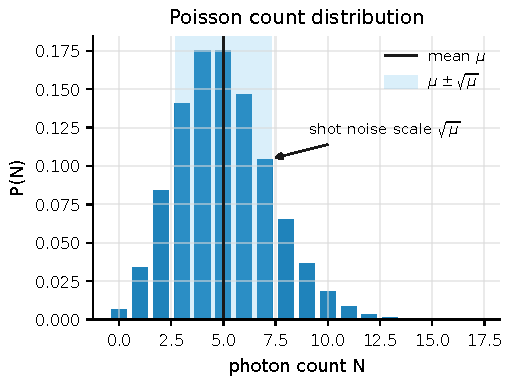
\includegraphics[width=0.86\linewidth]{figures/generated/chapter_01/ch01_photon_count_statistics.pdf}
\caption{Poisson 计数分布的基本形状。平均计数为 \(\mu\) 时，方差也是 \(\mu\)，shot noise 的尺度为 \(\sqrt{\mu}\)。}
\label{fig:chapter-01-02}
\end{figure}

\section{几个必须先记住的数量级}
\label{sec:1-scales}

第一，时间误差可以换成光程误差：
\begin{equation}
  \Delta \ell=c\,\Delta t .
  \label{eq:path-time}
\end{equation}
\begin{formulaexplain}
\(\Delta\ell\) 是光程误差；\(c\) 是光速；\(\Delta t\) 是计时误差或延迟误差。这条式子把时间同步精度直接换算成空间尺度。
\end{formulaexplain}
\(c\simeq3.0\times10^{10}\,{\rm cm\,s^{-1}}\) 是光速。\(1\,{\rm ps}\) 对应约 \(3.0\times10^{-2}\,{\rm cm}\)，\(1\,{\rm ns}\) 对应约 \(30\,{\rm cm}\)。所以只要讨论快速计时、几何延迟或两个站点的同步，时间单位马上会变成空间尺度。

第二，光子能量由频率或波长决定：
\begin{equation}
  E_\gamma=h\nu=\frac{hc}{\lambda}.
  \label{eq:photon-energy}
\end{equation}
\begin{formulaexplain}
\(E_\gamma\) 是单个光子的能量；\(h\) 是 Planck 常数；\(\nu\) 是频率；\(c\) 是光速；\(\lambda\) 是波长。它说明高频短波长光子携带更高能量。
\end{formulaexplain}
\(h\) 是 Planck 常数。蓝光光子比红光光子能量高；同样的能量流量，在红光中对应更多光子。把能量流量换成光子率时，必须除以 \(E_\gamma\)。

第三，带宽可以在频率和波长之间换算。对窄带近似，
\begin{equation}
  \Delta\nu\simeq \frac{c\,\Delta\lambda}{\lambda^2}.
  \label{eq:bandwidth-conversion}
\end{equation}
\begin{formulaexplain}
\(\Delta\nu\) 是频率带宽；\(\Delta\lambda\) 是波长带宽；\(\lambda\) 是中心波长；\(c\) 是光速。它给出窄带近似下波长分辨率和频率分辨率的换算。
\end{formulaexplain}
\(\Delta\lambda\) 是波长带宽。以 \(\lambda=500\,{\rm nm}\)、\(\Delta\lambda=1\,{\rm nm}\) 为例，\(\Delta\nu\simeq1.2\times10^{12}\,{\rm Hz}\)。后面讨论光谱通道和相干时间时，会反复用到这个换算。

第四，探测到的光子率可以粗略写成
\begin{equation}
  R_\gamma=A\eta\int F_\lambda\frac{\lambda}{hc}\,d\lambda .
  \label{eq:photon-rate}
\end{equation}
\begin{formulaexplain}
\(R_\gamma\) 是探测光子率；\(A\) 是有效收集面积；\(\eta\) 是总效率；\(F_\lambda\) 是谱流量密度；\(\lambda/(hc)\) 把能量流量换成光子数；积分表示对带宽求和。
\end{formulaexplain}
\(A\) 是有效收集面积，单位 \({\rm cm^2}\)；\(\eta\) 是系统总效率；\(F_\lambda\) 是谱流量密度；\(\lambda/(hc)\) 把能量流量换成光子数流量。这个式子告诉我们，目标亮度、望远镜面积、带宽和效率共同决定事件表里到底有多少光子。

\begin{longtable}{p{0.24\linewidth}p{0.30\linewidth}p{0.34\linewidth}}
\toprule
量 & 常见数量级 & 基本意义 \\
\midrule
\(\lambda\) & \(350\,{\rm nm}\) 到 \(1.6\,\mu{\rm m}\) & 观测波长。 \\
\(\nu\) & \(10^{14}\)--\(10^{15}\,{\rm Hz}\) & 光学频率。 \\
\(\Delta t\) & ps 到 s & 时间戳精度、bin 宽或曝光时间。 \\
\(R_\gamma\) & \(<1\) 到 \(10^9\,{\rm s^{-1}}\) & 单通道探测光子率。 \\
\(\mu\) & \(R_\gamma\Delta t\) & 一个 bin 中的平均计数。 \\
\(1/\sqrt{\mu}\) & 从很大到很小 & Poisson 相对噪声。 \\
\(\eta\) & \(0.01\) 到 \(0.5\) & 大气、光学和探测器总效率。 \\
\bottomrule
\end{longtable}

\chapter{为什么需要量子天文学}
\label{chap:02}

\begin{chapteropening}
普通天文学已经能给出图像、光谱、光变曲线和偏振。那为什么还需要“量子天文学”？本章要回答的核心问题是：当我们把光子事件压缩成平均强度以后，是否还有物理信息被丢掉了？

答案是有。平均强度告诉我们“有多少光”，但不一定告诉我们“这些光子怎样一起到达”。量子天文学不否定传统数据产品，而是回到更底层的光子事件表，保留到达时间、望远镜位置、频率、偏振和事件之间的联合概率。HBT、Narrabri、恒星 photon bunching、VERITAS 和 MAGIC 强度干涉已经说明，这类信息可以真实测量；它既不等同于量子引力，也不只是把光子一个个数出来 \citep{1956Natur.178.1046H,1974iiia.book.....H,2017MNRAS.472.4126G,2020NatAs...4.1164A,2024MNRAS.529.4387A}。
\end{chapteropening}

\section{普通天文学为什么会丢掉一部分信息}
\label{sec:2-classical-products}
\label{sec:2-lost-correlations}

第 \ref{chap:01} 章把一次光子探测写成事件行 \(e_j=(t_j,\bm r_j,\nu_j,p_j,w_j)\)。这里 \(t_j\) 是到达时间，\(\bm r_j\) 是接收位置或望远镜编号，\(\nu_j\) 是频率通道，\(p_j\) 是偏振标签，\(w_j\) 是权重。现在的问题是：当我们把这张表变成一幅图像、一条光谱或一条光变曲线时，哪些列被保留，哪些关系被平均掉？

先看最熟悉的图像。若把事件按角坐标 \((x,y)\) 分箱，像素面积为 \(\Delta\Omega\)，曝光时间为 \(\Delta t\)，频率带宽为 \(\Delta\nu\)，则该像素的平均亮度可估计为
\begin{equation}
  \hat I(x,y)\simeq
  \frac{N(x,y)}
       {A_{\rm eff}\,\eta\,\Delta t\,\Delta\nu\,\Delta\Omega}.
  \label{eq:ch02-image-intensity}
\end{equation}
\begin{formulaexplain}
\(\hat I(x,y)\) 是像素亮度估计；\(N(x,y)\) 是该像素光子数；\(A_{\rm eff}\)、\(\eta\)、\(\Delta t\)、\(\Delta\nu\)、\(\Delta\Omega\) 分别给出收集面积、效率、曝光时间、带宽和立体角。它说明普通图像把事件表压缩成一阶平均量。
\end{formulaexplain}
这里 \(N(x,y)\) 是该像素内的加权光子数；\(A_{\rm eff}\) 是有效收集面积，单位 \(\mathrm{cm^2}\)；\(\eta\) 是系统总效率；\(\Delta\Omega\) 的单位是 sr。这个公式做了一件很自然的事：把一个像素里的事件全部加起来，再除以收集面积、效率、时间、带宽和立体角。光谱是按 \(\nu\) 分箱，光变曲线是按 \(t\) 分箱，普通偏振是把不同偏振通道的平均强度组合成 Stokes 参数。它们都主要是一阶统计量。

一阶统计量回答的是“单个事件落在哪里”或“某个 bin 里总共有多少事件”。它不回答“两个事件是否倾向于一起出现”。例如，把 \(10^8\) 个事件压缩成一条光变曲线以后，我们仍然知道每个时间 bin 的总数，却不知道同一 bin 里的事件是否成对聚集、是否来自同一对望远镜、是否落在同一频率和偏振模式中。对许多天体物理问题，这种压缩完全足够；但对强度干涉、光子聚束、跨谱线相关、偏振相关和最优参数估计，它会把目标信号本身压掉。

\begin{figure}[tbp]
\centering
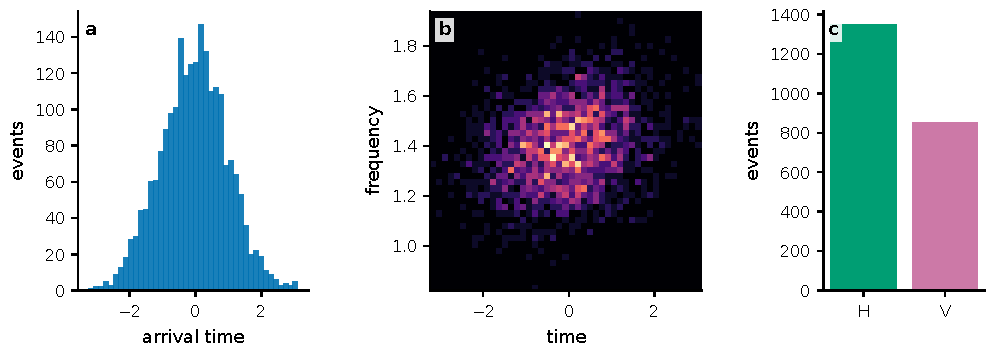
\includegraphics[width=0.92\linewidth]{figures/generated/chapter_02/ch02_event_table_information.pdf}
\caption{光子事件表把时间、望远镜位置、频率通道和偏振标签放在同一个数据结构中。按单一坐标边缘化得到光变曲线、谱线或偏振强度；保留两两事件关系则得到延迟直方图、强度相关函数和跨通道协方差。}
\label{fig:chapter-02-event-table}
\end{figure}

图 \ref{fig:chapter-02-event-table} 给出了这件事的数据图像。只保留单事件分布时，我们得到传统数据产品；保留事件对时，才开始看到延迟直方图、强度相关函数和跨通道协方差。量子天文学的第一个动机正是在这里：它不是先假设光有多“神秘”，而是先问事件表里是否有传统平均量没有使用的信息。

一个简单例子能说明这个差别。两束光可以有相同的平均强度和相同的光变曲线，但短时间延迟上的事件对数量不同。Poisson 光的到达近似彼此独立；热光在相干时间内有过量共同到达概率。这两者的平均亮度可以一样，但二阶统计不同。因此下一步要理解的不是“更多光子数”，而是“事件之间的联合概率”。

\section{怎样把“光子一起到达”写成可测量的量}
\label{sec:2-thermal-coherent}

物理上，相关就是“一个事件发生后，另一个事件发生的概率是否改变”。用 \(a\) 表示一个事件标签，它可以是时间 bin、望远镜编号、频率通道或偏振通道。一阶概率 \(P_1(a)\) 描述单个事件落入 \(a\) 的概率；二阶概率 \(P_2(a,b)\) 描述两个事件分别落入 \(a\) 和 \(b\) 的联合概率。若事件完全独立，就有
\begin{equation}
  P_2(a,b)=P_1(a)P_1(b).
  \label{eq:ch02-independent}
\end{equation}
\begin{formulaexplain}
\(P_1(a)\) 和 \(P_1(b)\) 是单事件概率；\(P_2(a,b)\) 是两个事件的联合概率。乘积形式表示完全独立到达；任何偏离它的部分才是相关信号。
\end{formulaexplain}
这条公式是“没有相关”的基线。任何偏离这个乘积的部分，都说明事件之间存在额外关系。

在实际数据里，我们通常数某个时间窗或某个延迟下的事件数。令 \(N_a\) 和 \(N_b\) 是两个通道中的计数，最直接的共同涨落量是协方差
\begin{equation}
  C_{ab}=\langle N_aN_b\rangle-\langle N_a\rangle\langle N_b\rangle.
  \label{eq:ch02-cov}
\end{equation}
\begin{formulaexplain}
\(C_{ab}\) 是通道 \(a,b\) 的协方差；\(N_a,N_b\) 是计数；第一项是真实共同涨落，第二项是独立到达时的平均乘积。它把“是否一起变亮或变暗”写成可测量的差值。
\end{formulaexplain}
尖括号表示对许多时间窗、许多实验重复或许多统计等价样本求平均。第一项 \(\langle N_aN_b\rangle\) 是实际共同出现的平均乘积；第二项是如果两个通道只按各自平均率独立到达时的期望。若 \(C_{ab}=0\)，通道间没有可测共同涨落；若 \(C_{ab}>0\)，有过量共同到达；若 \(C_{ab}<0\)，可能是死时间、pile-up、选择效应，也可能是更特殊的反聚束。

为了把不同亮度的源放在同一尺度上，常用归一化二阶相关函数
\begin{equation}
  g^{(2)}_{ab}(\tau)=
  \frac{\langle N_a(t)N_b(t+\tau)\rangle}
       {\langle N_a(t)\rangle\langle N_b(t+\tau)\rangle}.
  \label{eq:ch02-g2-count}
\end{equation}
\begin{formulaexplain}
\(g^{(2)}_{ab}(\tau)\) 是延迟 \(\tau\) 下的归一化二阶相关；分子数跨通道事件对，分母给出随机符合基线。它把不同亮度、不同计数率的数据放到同一相关尺度上。
\end{formulaexplain}
\(\tau\) 是两个通道之间的延迟，单位秒。这个量可以从事件表直接估计：构造 \(a\) 通道和 \(b\) 通道的事件对延迟直方图，再除以由两个单通道平均计数率给出的随机符合。\(g^{(2)}=1\) 是独立到达；\(g^{(2)}>1\) 表示聚束或共同涨落；\(g^{(2)}<1\) 则必须同时考虑非经典反聚束和仪器效应。

有了这个归一化尺度，前面那个“平均亮度相同、事件关系不同”的例子就可以画出来。两束光在一阶统计上可以完全一样：同样的平均强度，同样的慢变光变曲线，同样的总光子数。但如果一束光的事件近似独立到达，另一束光在相干时间内更容易成对到达，它们的 \(g^{(2)}\) 曲线就不同。

\begin{figure}[tbp]
\centering
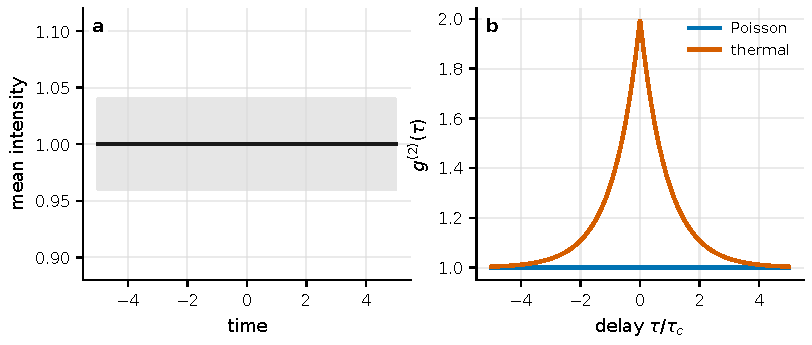
\includegraphics[width=0.92\linewidth]{figures/generated/chapter_02/ch02_mean_intensity_vs_correlation.pdf}
\caption{两束光可以有相同平均强度，却有不同的二阶相关函数。Poisson 光的 \(g^{(2)}\) 近似为 1；热光在相干时间内有过量共同到达概率，表现为 \(g^{(2)}(0)>1\)。}
\label{fig:chapter-02-mean-vs-correlation}
\end{figure}

这种差别来自光场状态本身。理想相干光的到达近似 Poisson 过程，知道平均率以后，一个光子的到来不改变同一模式中下一个光子的即时到达概率，因此零延迟相关为 1。单模热光有额外强度涨落：场强偏高的一小段时间里，多个光子都会更容易到达，于是零延迟附近的事件对多于随机基线，理想极限为 2。单模成对因子 \(b_2\) 给出这两个基准值，见式 \eqref{eq:ch03-coherent} 和式 \eqref{eq:ch03-thermal-density}；事件表中的归一化二阶相关把同一物理写成 \(g^{(2)}\)。

真实天体观测很少只收集一个模式。频率带宽、时间门宽、空间模式、偏振和背景都会把许多独立涨落平均到一起，使 \(g^{(2)}-1\) 变小。最重要的直觉是：随机符合基线随总光子数快速增长，真正携带聚束信息的同模涨落只占其中很小一部分。相干时间大约由光学带宽决定，带宽越宽，相干时间越短；若探测器或分析 bin 远慢于相干时间，聚束峰会被平均到 \(10^{-3}\)、\(10^{-6}\) 甚至更低。多模和时间响应的定量写法放在第 \ref{chap:04} 章式 \eqref{eq:ch04-multimode} 和式 \eqref{eq:ch04-contrast-dilution}。

\begin{figure}[tbp]
\centering
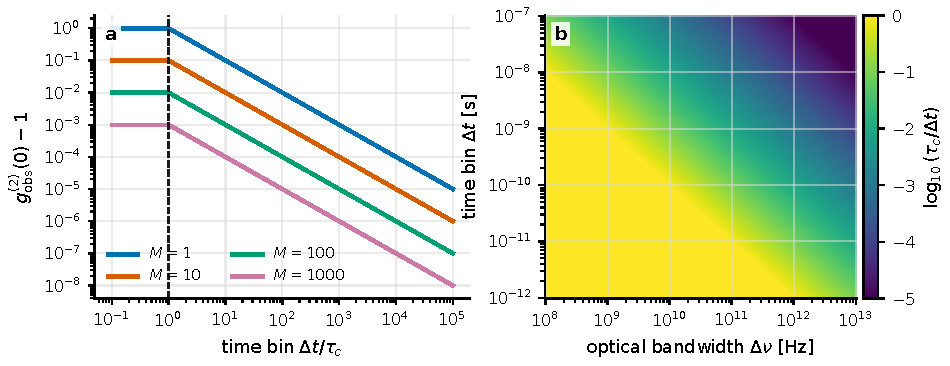
\includegraphics[width=0.92\linewidth]{figures/generated/chapter_02/ch02_contrast_dilution.pdf}
\caption{二阶相关对比度会被有效模式数和时间分辨率同时压低。左图显示模式数 \(M\) 增大或时间 bin \(\Delta t\) 大于相干时间 \(\tau_c\) 后，\(g^{(2)}_{\rm obs}(0)-1\) 快速下降。右图把 \(\tau_c\simeq1/\Delta\nu\) 代入，显示宽光学带宽和慢电子响应会把聚束峰压到很小。}
\label{fig:chapter-02-dilution}
\end{figure}

图 \ref{fig:chapter-02-dilution} 给出望远镜里的数量级。若 \(\Delta\nu=10^{12}\,\mathrm{Hz}\)，则 \(\tau_c\sim1\,\mathrm{ps}\)；若电子响应是 \(1\,\mathrm{ns}\)，即使是单模、单偏振热光，相关峰也只剩约 \(10^{-3}\)。再乘上多模、背景和偏振稀释，天文数据中的目标信号常常低到 \(10^{-6}\) 到 \(10^{-3}\)。这解释了为什么强度相关不是“看起来相关就行”，而是一项严肃的误差预算问题。

\section{HBT 为什么能测天体大小，又为什么长期困难}
\label{sec:2-hbt-history}
\label{sec:2-revival}

到这里我们知道了二阶相关能测“共同涨落”。HBT 是 Hanbury Brown--Twiss 的缩写，来自 R. Hanbury Brown 和 R. Q. Twiss 在 1950 年代提出并验证的强度干涉思想。这个想法先在实验室 photon correlation 中引起争论和确认，随后被用于 Sirius 的恒星测试，最后发展成 Narrabri Stellar Intensity Interferometer，并给出一批明亮恒星的角直径 \citep{1956Natur.177...27B,1957RSPSA.242..300B,1956Natur.178.1046H,1958RSPSA.248..222B,1974iiia.book.....H}。

把两台望远镜想成两个相距很远的光子计数器，它们都指向同一颗恒星。恒星表面的每一个小面元都像一个很小的热光源，发出的电场相位快速而随机地抖动。来自同一个小面元的光会同时到达两台望远镜，只是到达第二台时多走了一点路，因此多带一个几何相位。来自另一个小面元的光也会同时到达两台望远镜，但它的几何相位又不同。

如果恒星在这条基线上看起来很小，所有小面元给出的几何相位差几乎一样，两台望远镜收到的电场仍然很相似。如果恒星已经被分辨，不同小面元给出的相位差分散开，平均时互相抵消，两台望远镜收到的电场相似度就下降。角直径的信息就藏在这个下降速度里：基线越长，越容易看出恒星不是一个点。

普通振幅干涉把两路光在光学上合并，让电场相加，再从条纹对比度读出这种相似度。HBT 保留两路光各自的探测记录，然后比较两路光强涨落是不是同步。同步得强，说明两台望远镜接收到的热光模式仍然相似；同步得弱，说明这条基线已经分辨了源的角结构。

现在把“电场相似度”写成一个量。若第 \(i,j\) 个接收位置的窄带复电场分别为 \(E_i(t)\) 和 \(E_j(t)\)，一阶互相干函数和归一化一阶相干度定义为
\begin{equation}
  \begin{aligned}
    \Gamma^{(1)}_{ij}(\tau)
    &=
    \langle E_i^*(t)E_j(t+\tau)\rangle,\\
    \gamma^{(1)}_{ij}(\tau)
    &=
    \frac{\Gamma^{(1)}_{ij}(\tau)}
         {\sqrt{\Gamma^{(1)}_{ii}(0)\Gamma^{(1)}_{jj}(0)}},\\
    \langle I_i\rangle
    &=
    \kappa_i\,\Gamma^{(1)}_{ii}(0).
  \end{aligned}
  \label{eq:ch02-first-order-coherence}
\end{equation}
\begin{formulaexplain}
\(\Gamma^{(1)}_{ij}\) 是两处电场的互相关；\(\gamma^{(1)}_{ij}\) 是归一化的一阶相干度；\(\langle I_i\rangle\) 是第 \(i\) 路观测到的平均光强；\(\kappa_i\) 把场强平方换成探测器记录的光强或计数率。
\end{formulaexplain}
式 \eqref{eq:ch02-first-order-coherence} 的读法很直接。\(\Gamma^{(1)}_{ij}\) 把两处电场相乘再平均；两处电场的相位关系越稳定，平均后留下的量越大。对角项 \(\Gamma^{(1)}_{ii}(0)=\langle E_i^*(t)E_i(t)\rangle\) 是第 \(i\) 路平均光强对应的场强平方平均；探测器真正记录的是 \(\langle I_i\rangle\)，两者只差效率、带宽、增益和单位选择等比例因子。分母用两个对角项归一化，\(\gamma^{(1)}_{ij}\) 便只保留相干性的大小和相位。对两台望远镜取 \(i=1,j=2\)，\(|\gamma^{(1)}_{12}|=1\) 表示两处电场完全相干，\(|\gamma^{(1)}_{12}|=0\) 表示平均后没有共同相位关系留下。

\(\gamma^{(1)}_{12}\) 可以由振幅干涉测到，条件是仪器保存两路电场并把它们合并。单路探测器只给出 \(\Gamma^{(1)}_{11}(0)\) 或 \(\Gamma^{(1)}_{22}(0)\) 这样的平均强度项；两束光相加后，输出光强里会出现交叉项。若在其中一路加入可控相位 \(\varphi\)，合并后的平均光强可写成
\[
  I_{\rm comb}(\varphi)
  \propto
  \Gamma^{(1)}_{11}(0)+\Gamma^{(1)}_{22}(0)
  +2\,{\rm Re}\!\left[e^{i\varphi}\Gamma^{(1)}_{12}(0)\right].
\]
改变 \(\varphi\) 时，条纹对比度给出 \(|\gamma^{(1)}_{12}|\)，条纹位置给出 \(\arg\gamma^{(1)}_{12}\)。所以普通光学或射电振幅干涉测到的复可见度，本质上就是 \(\gamma^{(1)}_{12}\)。

HBT 的数据流不同。每台望远镜先把光变成光电流或光子事件表；随后把几何延迟校正掉，再问一个非常具体的问题：第一路在某个时刻偏亮时，第二路在相同延迟处是否也偏亮？连续光电流可以相乘平均；光子事件表则构造两路事件对的延迟直方图，再除以同样计数率和同样 live time 下的随机符合数。这个估计量的完整写法放在第 \ref{chap:04} 章式 \eqref{eq:ch04-g2-estimator}。

热光有一个关键性质：同一个模式会一阵亮、一阵暗。两台望远镜若接收到相干的同一批模式，就会一起看到这些亮暗起伏；两处电场越相似，强度涨落越同步。对高斯混沌热光，这句话由 Siegert 关系定量表达：强度相关的 excess 正比于一阶相干度的模平方。它的四阶矩推导见第 \ref{chap:04} 章式 \eqref{eq:ch04-siegert}；在空间 HBT 中，对应关系见第 \ref{chap:05} 章式 \eqref{eq:ch05-hbt-spatial}。物理读法是：HBT 从光强涨落读出的量，正是普通振幅干涉会称为“可见度”的模平方，真实观测还要乘上时间响应、模式、偏振和背景稀释因子。

还差最后一步：\(\gamma^{(1)}_{12}\) 为什么包含恒星大小？把恒星表面分成许多小面元。每个面元都像一个很小的点源，来自不同面元的热光彼此独立；因此求平均时，只有“同一个面元到达两台望远镜”的相关项留下来。一个面元越亮，它留下的相关项权重越大；一个面元方向越偏，它的几何相位转得越快。把所有面元按亮度加权相加，就得到 van Cittert--Zernike 定理：空间相干度是天空亮度的归一化 Fourier 分量。第 \ref{chap:05} 章式 \eqref{eq:ch05-vcz} 会给出完整公式和适用边界。

这条关系让强度干涉能测角大小。若源很小，各面元的相位几乎排在一起，\(|\gamma^{(1)}_{12}|^2\) 接近 1；若源被基线分辨，不同方向的相位互相抵消，\(|\gamma^{(1)}_{12}|^2\) 随基线下降。均匀圆盘会给出熟悉的 Bessel 型可见度曲线，第一零点和下降速度直接编码角直径；具体公式、第一零点和非均匀模型放在第 \ref{chap:05} 章式 \eqref{eq:ch05-uniform-disk} 之后讨论。

Sirius 测试和 Narrabri 强度干涉仪把这个方法带入天文学。Narrabri 使用两台 6.5 m 光收集器，测量热星角直径，并最终给出 32 颗恒星的角直径目录；后续工作还讨论了边缘昏暗如何影响从均匀圆盘直径到真实恒星直径的修正 \citep{1956Natur.178.1046H,1967MNRAS.137..375H,1967MNRAS.137..393H,1974MNRAS.167..121H,1974MNRAS.167..475H,1974iiia.book.....H}。HBT 的影响也超出天文学。Baym 的综述从恒星讲到核碰撞，说明同样的二粒子相关思想可以把“源的空间尺度”映射到“相关函数的宽度” \citep{1998AcPPB..29.1839B,1990RvMP...62..553B}。

那为什么这种方法后来沉寂了很久？主要原因是信号太小。强度干涉的相关峰要从巨大的随机符合背景中捞出来；提高信噪比最直接的资源是更大的收集面积、更高的量子效率、更宽的电子带宽和更长的积分时间，而这些资源只会以不同速度改善误差。经典 SNR 标度式和观测设计用法放在第 \ref{chap:05} 章式 \eqref{eq:ch05-snr} 和第 \ref{chap:18} 章。它的物理含义是：HBT 放宽了光学相位稳定要求，却把压力转移到光子数、时间响应、背景和系统误差预算上。

现代复兴主要靠工程条件变化。大口径 Cherenkov 望远镜阵列提供了现成的大收集面积；PMT、APD、SPAD 和高速电子学可以在 ns 到 ps 尺度记录涨落；FPGA/GPU 和离线相关允许把多台望远镜的数据流复制到许多基线组合中；精密时间同步和数字延迟校正可以跟踪几何光程差，而不必把光学相位稳定到纳米尺度。Le Bohec--Holder、Dravins--CTA 和后来的 CTA 布局模拟给出的工程路线很一致：信号弱，但电子相关器可以复制，粗糙光学也能工作，多台望远镜会把 \(u,v\) 覆盖变成主要资产 \citep{2006ApJ...649..399L,2008AIPC..984..205L,2012NewAR..56..143D,2013APh....43..331D,2010SPIE.7734E..1CN,2010SPIE.7734E..1TJ}。

现代实测已经越过“概念可行”阶段。Guerin 等人用 1 m 望远镜在 photon-counting 模式下测到 Arcturus、Procyon 和 Pollux 的时间 photon bunching，相关峰对比度约 \(2\times10^{-3}\)，噪声接近 shot-noise 标度 \citep{2017MNRAS.472.4126G}。VERITAS 四台 12 m Cherenkov 望远镜的强度干涉系统测量了 \(\beta\) CMa 和 \(\epsilon\) Ori 的亚毫角秒角直径，精度优于 5\%，并展示了多基线离线相关的可扩展性 \citep{2020NatAs...4.1164A}。MAGIC 两台 17 m Cherenkov 望远镜也完成了光学强度干涉观测，后续系统论文给出了性能和第一批测量结果 \citep{2020MNRAS.491.1540A,2024MNRAS.529.4387A}。Aqueye/Iqueye 的 Vega photon-counting 实验则展示了高时间分辨事件表、零基线相关和公里级基线校准中的系统误差问题 \citep{2021MNRAS.506.1585Z}。

\begin{figure}[tbp]
\centering
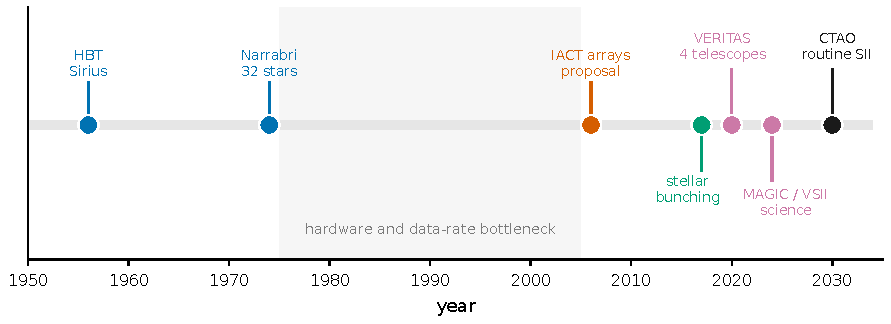
\includegraphics[width=0.92\linewidth]{figures/generated/chapter_02/ch02_revival_timeline.pdf}
\caption{光学强度干涉从 HBT 和 Narrabri 到 Cherenkov 阵列复兴的时间线。1970 年代之后的沉寂主要来自大面积光收集器、高速探测和多基线相关器的工程瓶颈；IACT 阵列、数字相关和 photon-counting 事件表把这些瓶颈逐步移开。}
\label{fig:ch02-revival-timeline}
\end{figure}

这条历史给本书一个很实际的判断：强度相关不是概念上不可行，而是需要足够光子数、足够稳定的时间系统、足够强的 null test 和足够诚实的误差预算。

\section{什么算量子天文学，第一代问题在哪里}
\label{sec:2-definition}
\label{sec:2-first-cases}

有了上面的例子，就可以给出本书的工作定义。量子天文学是一类事件层面的观测问题：研究天体光场的联合概率、相干函数和模式信息，并用这些量处理天体物理、传播效应、基础物理或观测设计。它的基本数据是带标签的光子事件表，而不只是平均强度数据产品。高速光子计时仪器如 Iqueye/Aqueye 的设计初衷，就是把天文光子作为带纳秒或更高时间精度的事件来处理 \citep{2010SPIE.7702E..0MC}。

更一般地，光电探测可以按一重、二重、三重乃至更高阶符合来组织。\(n=1\) 给出普通平均强度，\(n=2\) 给出 HBT 和 photon bunching，\(n=3\) 可在多望远镜强度干涉中帮助恢复部分相位信息。场算符和光态给出这些符合统计的量子来源；事件表和相关估计量给出它们的观测实现。它们都对应可估计的符合统计。

这个边界很实用。量子天文学不等于量子引力，也不等于任何使用“量子”二字的宇宙学讨论。一个问题若不能写成事件表中的可估计量、误差模型和 null test，就还不是可执行的观测项目。反过来，普通 photon counting 也不自动属于量子天文学；只有当单光子事件的联合统计、模式结构或最优测量比平均强度提供额外信息时，它才进入这个范围。

第一代最稳妥的科学目标是明亮恒星。强度干涉可以测角直径、边缘昏暗、快速自转引起的扁率、双星分离和热星风结构。恒星足够亮，近似热光，角尺度在 \(0.05\) 到数 mas，正好落在百米到公里级可见光基线的敏感范围。Narrabri 的历史结果、VERITAS/MAGIC 的现代直径测量、\(\beta\) UMa 角直径和 \(\gamma\) Cas 扁率结果，都把这类目标推到第一代观测的最前面 \citep{1974MNRAS.167..121H,2020NatAs...4.1164A,2024MNRAS.529.4387A,2024ApJ...966...28A,2025ApJ...995..191A}。

时间结构明显的源提供另一条路线。脉冲星、爆发源、nova、supernova 和微透镜事件把到达时间放到中心位置。若两个未分辨光路有微小时间延迟，photon bunching 的延迟结构可能携带额外信息。Saha 提出用 photon bunching 测微透镜质量，Lewis 和 Tuthill 随后讨论 decoherence 对这种设想的影响，说明这类想法需要同时处理相干时间、源尺寸和传播路径差 \citep{2019MNRAS.486.5400S,2020MNRAS.491.5789L}。

频率和偏振相关则把问题推向辐射机制。谱线内外的 \(g^{(2)}(\tau)\) 可以连接到相干时间和谱宽；偏振分辨相关可以测试辐射机制、磁场几何和传播效应。自然 laser 的 photon-correlation spectroscopy、黑体 photon bunching 和 X-ray driven photon bunching 都显示，HBT 思想不只属于恒星角直径，也可以成为谱线宽度、激发过程和高能闪烁的诊断工具 \citep{2005NewA...10..361J,2008AIPC..984..216D,2014ApJ...789L..10T,2024arXiv241216975K}。这些方向离常规巡天更远，但物理链条仍然从事件表开始，经过光子统计，再进入辐射机制、传播效应和基础物理。

\begin{figure}[tbp]
\centering
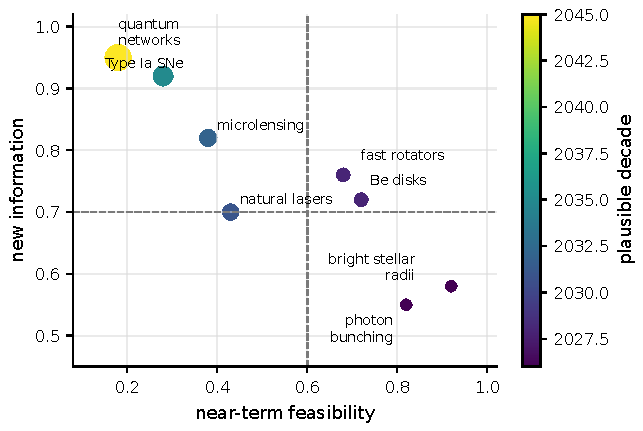
\includegraphics[width=0.76\linewidth]{figures/generated/chapter_02/ch02_science_case_map.pdf}
\caption{第一代量子天文学科学问题的可行性和新增信息量。亮星角直径和恒星 photon bunching 已经靠近常规观测；Be 星盘、快速自转星和自然 laser 属于近期扩展；Type Ia 超新星角距离和量子网络望远镜科学价值高，但需要更长基线、快速触发或量子链路工程。}
\label{fig:ch02-science-map}
\end{figure}

\begin{longtable}{p{0.22\linewidth}p{0.30\linewidth}p{0.36\linewidth}}
\toprule
观测量 & 典型范围 & 主要限制 \\
\midrule
\(R_\gamma\) & \(10^5\) 到 \(10^9\,\mathrm{s^{-1}}\) 对亮星单通道可达 & 探测器饱和、死时间、背景和数据率。 \\
\(\Delta t\) & \(10\,\mathrm{ps}\) 到 \(10\,\mathrm{ns}\) & 探测器抖动、电子带宽、镜面等时性和时钟同步。 \\
\(\Delta\nu\) & \(10^9\) 到 \(10^{13}\,\mathrm{Hz}\) & 窄带提高相干时间但降低光子率；宽带相反。 \\
\(g^{(2)}-1\) & \(10^{-6}\) 到 \(10^{-3}\) 常见于天文强度干涉 & 模式数、时间稀释、偏振稀释和背景稀释。 \\
\(B\) & \(10\,\mathrm{m}\) 到 \(10\,\mathrm{km}\) & 决定角尺度；长基线信号小，需要更多光子和更准模型。 \\
\(|\gamma^{(1)}|^2\) & 0 到 1 & 源被分辨后下降；只测模平方时相位恢复困难。 \\
\bottomrule
\end{longtable}

\chapter{量子光学基础}
\label{chap:03}

\begin{chapteropening}
望远镜收到的是一串点击事件，但这些点击从哪里来？本章的中心问题是：怎样从“光场的状态”走到“探测器记录的事件表”，并判断哪些统计量能在天文观测中保留下来。

最有用的起点不是把光想成一团连续能量，而是把光分解成模式。每个模式有频率、空间形状、偏振和时间范围；光子是模式的激发；探测器记录的是这些模式被吸收后留下的点击。数态、相干态、热态和压缩态分别回答光子数是否固定、相位是否稳定、强度是否涨落、噪声是否能在两个正交分量之间重新分配。单模光子数统计给出成对到达的基线，也决定相关函数在零延迟处的物理含义 \citep{1963PhRv..130.2529G,1963PhRv..131.2766G,1965RvMP...37..231M,1995ocqo.book.....M,1997quop.book.....S,2001qops.book.....S,2013quop.book.....A}。
\end{chapteropening}

\section{望远镜接收到的“一个光子”属于哪个模式}

现在的问题是：当探测器记录一个点击时，这个点击对应的是哪一个自由度？答案不是“一个没有结构的小球”，而是某个光学模式的一次激发。模式可以按频率、时间窗、空间形状、到达方向和偏振来定义。一个窄带、衍射受限、单偏振、持续一个相干时间的场自由度，就是最接近“单模式”的天文例子。

在量子光学里，正频率电场算符可按一组正交模式展开：
\begin{equation}
  \hat E^{(+)}(\bm{r},t)=\sum_k {\cal E}_k u_k(\bm{r})e^{-i\omega_k t}\hat a_k .
  \label{eq:ch03-field-expansion}
\end{equation}
\begin{formulaexplain}
\(\hat E^{(+)}\) 是正频率场算符；\(k\) 标记频率、空间形状和偏振等模式；\({\cal E}_k\) 是模式归一化因子；\(u_k\) 是模式函数；\(\omega_k\) 是角频率；\(\hat a_k\) 是湮灭算符。它把望远镜收到的光写成各个模式的量子激发。
\end{formulaexplain}
这里 \(\hat E^{(+)}\) 是正频率电场算符；\(\bm r\) 是位置，单位厘米；\(t\) 是时间，单位秒；\(\omega_k=2\pi\nu_k\) 是第 \(k\) 个模式的角频率，单位 \(\mathrm{rad\,s^{-1}}\)；\(u_k(\bm r)\) 是空间模式函数；\(\hat a_k\) 是该模式的湮灭算符。标签 \(k\) 不是一个简单序号，而是一整套模式标签：频率、带宽、空间模式、偏振和时间窗。采用不同归一化时，\({\cal E}_k\) 和 \(u_k\) 的量纲可以重新分配，但 \(\hat a_k\) 的量子代数不变。

为什么要引入 \(\hat a_k\)？因为光电探测本质上是在某个模式中减少一个光子。正交模式的产生和湮灭算符满足
\begin{equation}
  [\hat a_i,\hat a_j^\dagger]=\delta_{ij},\qquad
  \hat n_i=\hat a_i^\dagger\hat a_i .
  \label{eq:ch03-commutator}
\end{equation}
\begin{formulaexplain}
\(\hat a_i^\dagger\) 和 \(\hat a_i\) 分别产生、湮灭第 \(i\) 个模式的光子；\(\delta_{ij}\) 表示正交模式；\(\hat n_i\) 是光子数算符。这个对易关系定义了“一个模式里数光子”的量子规则。
\end{formulaexplain}
\(\hat a_i^\dagger\) 往第 \(i\) 个模式里增加一个光子，\(\hat a_i\) 从这个模式里取走一个光子，\(\hat n_i\) 是该模式的光子数算符，本征值 \(N=0,1,2,\ldots\) 没有单位。\(\delta_{ij}\) 表示只有同一模式的产生和湮灭顺序会留下量子修正。望远镜不会直接读出 \(\hat a\) 或 \(\hat E\)，它读出时间戳、像素、能量通道和偏振通道；这些记录是 \(\hat n\) 或多个 \(\hat n\) 的相关函数经过仪器响应后的结果。

天文观测通常不是单模式。若探测窗口长为 \(\Delta t\)，光谱带宽为 \(\Delta\nu\)，望远镜接收的有效光展量为 \(A\Omega\)，偏振通道数为 \(N_{\rm pol}\)，粗略的模式数可写成
\begin{equation}
  M \simeq
  \left(\frac{\Delta t}{\tau_c}\right)
  \left(\frac{A\Omega}{\lambda^2}\right)
  N_{\rm pol},
  \qquad
  \tau_c\simeq\frac{1}{\Delta\nu}\simeq\frac{\lambda^2}{c\,\Delta\lambda}.
  \label{eq:ch03-effective-modes}
\end{equation}
\begin{formulaexplain}
\(M\) 是有效模式数；\(\Delta t/\tau_c\) 数时间模式；\(A\Omega/\lambda^2\) 数空间模式；\(N_{\rm pol}\) 数偏振模式；\(\tau_c\) 是相干时间。它说明实际天文通道常是许多模式的平均。
\end{formulaexplain}
式 \eqref{eq:ch03-effective-modes} 的推法是把可分辨的相空间格子数相乘。一个频带宽度 \(\Delta\nu\) 的波包相干时间约为 \(\tau_c\simeq1/\Delta\nu\)，所以长度为 \(\Delta t\) 的时间窗包含约 \(\Delta t/\tau_c\) 个独立时间模式。空间上，一个衍射受限单模式占据的光展量约为 \(\lambda^2\)，望远镜和后端孔径共接收 \(A\Omega\)，所以空间模式数约为 \(A\Omega/\lambda^2\)。若偏振没有被投影到单一通道，还要乘上偏振模式数 \(N_{\rm pol}\)。最后，\(\nu=c/\lambda\) 给出 \(\Delta\nu\simeq c\,\Delta\lambda/\lambda^2\)，因此 \(\tau_c\simeq\lambda^2/(c\,\Delta\lambda)\)。

\(\Delta t\) 和 \(\tau_c\) 都用秒；\(A\Omega\) 的单位是 \(\mathrm{cm^2\,sr}\)；\(\lambda\) 是波长。式 \eqref{eq:ch03-effective-modes} 只是数量级计数，不是严格的整数公式：真实模式数还会受滤光片形状、点扩散函数、光纤耦合、像素大小和偏振选择影响。衍射受限单空间模式满足 \(A\Omega\sim\lambda^2\)，seeing-limited 光纤或大像素会接收很多空间模式。以 \(\lambda=500\,\mathrm{nm}\)、\(\Delta\lambda=1\,\mathrm{nm}\) 为例，\(\Delta\nu\simeq1.2\times10^{12}\,\mathrm{Hz}\)，所以 \(\tau_c\) 只有约 \(0.8\,\mathrm{ps}\)。若探测器时间响应是 \(100\,\mathrm{ps}\) 到 \(1\,\mathrm{ns}\)，一个时间 bin 已经平均了上百到上千个时间模式 \citep{2000stop.book.....G,1956Natur.177...27B,1957RSPSA.242..300B,1974iiia.book.....H}。

这说明一个重要事实：天文数据中的“一个通道”常常不是一个量子模式，而是许多模式的总和。后面的光子统计、聚束幅度和非经典信号都会被这个模式数稀释。

\section{不同光态怎样改变点击统计}

知道了模式，下一步要问：同一个模式里可以有什么样的光态？最简单的区别不是总光子率，而是计数分布和成对概率。对单模式计数，零延迟成对倾向可用
\[
  b_2\equiv
  \frac{\langle \hat n(\hat n-1)\rangle}{\langle\hat n\rangle^2}.
\]
\(b_2=1\) 是独立 Poisson 到达的基线；\(b_2>1\) 表示聚束；\(b_2<1\) 表示反聚束。数态、相干态和热态即使有相同平均光子数，也会给出不同的 \(P(N)\) 和不同的 \(b_2\)。

数态 \(|n\rangle\) 是光子数算符的本征态：
\begin{equation}
  P_{\rm Fock}(N)=\delta_{Nn},\qquad
  b_2=1-\frac{1}{n}.
  \label{eq:ch03-fock}
\end{equation}
\begin{formulaexplain}
\(P_{\rm Fock}(N)\) 是数态的计数概率；\(\delta_{Nn}\) 表示只可能数到 \(n\) 个光子；\(\hat n\) 是光子数算符；\(b_2\) 衡量同一模式内可组成的光子对数相对独立到达基线的大小。它给出反聚束的理想极限。
\end{formulaexplain}
这里 \(P(N)\) 是数到 \(N\) 个光子的概率。数态的推导最直接：若每次测量都得到 \(N=n\)，则
\[
  \langle \hat n\rangle=n,
  \qquad
  \langle \hat n(\hat n-1)\rangle=n(n-1).
\]
代入成对因子的阶乘矩定义，
\[
  b_{2,{\rm Fock}}
  =
  \frac{n(n-1)}{n^2}
  =
  1-\frac{1}{n}.
\]
单光子态 \(n=1\) 给 \(b_2=0\)，表示不可能在同一模式中同时探测到两个光子，这是反聚束的极限。天体光很少以纯数态到达，因为源区、传播路径和仪器都会混合未观测自由度；但数态告诉我们，点击统计测的是光子数相关，而不是一条连续波形 \citep{1977PhRvL..39..691K,1979OptL....4..205M,1998RvMP...70..101P}。

相干态 \(|\alpha\rangle\) 是稳定相位振荡的理想模型，满足 \(\hat a|\alpha\rangle=\alpha|\alpha\rangle\)。它的平均光子数是 \(\bar n=|\alpha|^2\)，单模计数服从 Poisson 分布：
\begin{equation}
  P_{\rm coh}(N)=e^{-\bar n}\frac{\bar n^N}{N!},
  \qquad
  \operatorname{Var}(N)=\bar n,\qquad
  b_2=1.
  \label{eq:ch03-coherent}
\end{equation}
\begin{formulaexplain}
\(P_{\rm coh}(N)\) 是相干态的 Poisson 计数分布；\(\bar n\) 是平均光子数；\(N!\) 是离散计数归一化；\(\operatorname{Var}(N)=\bar n\) 表示 shot noise；\(b_2=1\) 表示没有额外聚束。
\end{formulaexplain}
\(\alpha\) 是无量纲复振幅；它的模平方给出每个模式的平均光子数，辐角 \(\arg\alpha\) 给出相位。为什么 Poisson 计数会给 \(b_2=1\)？对一个时间窗内的单模计数，成对因子可以写成阶乘矩
\[
  b_2
  =
  \frac{\langle N(N-1)\rangle}{\langle N\rangle^2}.
\]
Poisson 分布的平均数为 \(\bar n\)，其二阶阶乘矩为
\[
  \begin{aligned}
  \langle N(N-1)\rangle
  &=
  \sum_{N=0}^{\infty}N(N-1)e^{-\bar n}\frac{\bar n^N}{N!}  \\
  &=
  e^{-\bar n}\bar n^2
  \sum_{N=2}^{\infty}\frac{\bar n^{N-2}}{(N-2)!}
  =
  \bar n^2 .
  \end{aligned}
\]
代回定义就得到
\[
  b_{2,{\rm coh}}
  =
  \frac{\bar n^2}{\bar n^2}=1 .
\]
这一步的物理意思是：扣除“同一个光子不能被数两次”的自配对以后，Poisson 光的光子对数正好等于独立到达给出的随机基线。看到一个光子，并不会提高同一模式中马上再看到一个光子的条件概率。稳定实验室激光在许多测量中接近相干态；天体窄线或高亮温源却不自动是相干态，因为独立发射区、速度场和散射路径会把相位平均掉。

热态是天体连续谱最常用的起点。单模热态的密度矩阵为
\begin{equation}
  \rho_{\rm th}=\sum_{N=0}^{\infty}
  \frac{\bar n^N}{(1+\bar n)^{N+1}}|N\rangle\langle N|,
  \qquad
  \operatorname{Var}(N)=\bar n(1+\bar n),\qquad
  b_2=2.
  \label{eq:ch03-thermal-density}
\end{equation}
\begin{formulaexplain}
\(\rho_{\rm th}\) 是热态密度矩阵；\(|N\rangle\) 是 \(N\) 光子数态；\(\bar n\) 是单模平均占有数；\(\operatorname{Var}(N)\) 是计数方差。它说明热光是光子数混合态，并自然产生 \(b_2=2\) 的聚束。
\end{formulaexplain}
这里 \(\bar n\) 是单模式平均占有数，不是望远镜每秒收到的总光子率。热态没有固定相位，是光子数基底上的混合态。式 \eqref{eq:ch03-thermal-density} 中的计数分布是几何分布。它的平均和方差为
\[
  \langle N\rangle=\bar n,
  \qquad
  \operatorname{Var}(N)=\langle N^2\rangle-\langle N\rangle^2
  =\bar n(1+\bar n).
\]
二阶相关需要的是 \(\langle N(N-1)\rangle\)，而不是普通的 \(\langle N^2\rangle\)。二者关系为
\[
  \langle N(N-1)\rangle
  =
  \langle N^2\rangle-\langle N\rangle
  =
  \operatorname{Var}(N)+\langle N\rangle^2-\langle N\rangle .
\]
把热态的平均和方差代入，
\[
  \langle N(N-1)\rangle
  =
  \bar n(1+\bar n)+\bar n^2-\bar n
  =
  2\bar n^2 ,
\]
所以
\[
  b_{2,{\rm th}}
  =
  \frac{2\bar n^2}{\bar n^2}=2 .
\]
这多出来的一倍不是探测器效应，而是热光强度涨落本身带来的成对概率增强：某一小段时间里强度偏高时，多个光子会一起更容易到来；强度偏低时，它们又一起变少。多模热光会把这种过量方差平均掉，使实际观测到的聚束对比度小于单模理想值 \citep{1965RvMP...37..231M,1995ocqo.book.....M,2000stop.book.....G,2017MNRAS.472.4126G,2024arXiv240418606N}。

\begin{figure}[tbp]
\centering
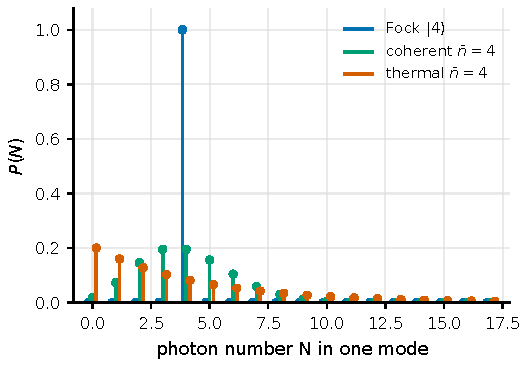
\includegraphics[width=0.82\linewidth]{figures/generated/chapter_03/ch03_state_count_distributions.pdf}
\caption{同一单模平均光子数附近，数态、相干态和热态给出完全不同的计数分布。数态的光子数固定，相干态的宽度为 \(\sqrt{\bar n}\)，热态有更长的高光子数尾部，所以会产生 \(b_2>1\) 的聚束信号。}
\label{fig:ch03-count-distributions}
\end{figure}

图 \ref{fig:ch03-count-distributions} 的物理意思很简单：平均光子数不是全部。数态没有光子数涨落；相干态有 Poisson 涨落；热态有额外强度涨落。天文强度干涉利用的正是最后这种热光涨落。

压缩态说明另一件事：量子噪声可以在两个正交场分量之间重新分配。定义
\begin{equation}
  \hat X_\theta=\frac{1}{2}\left(\hat a e^{-i\theta}+\hat a^\dagger e^{i\theta}\right),
  \qquad
  \Delta X_{\rm sq}^2=\frac{1}{4}e^{-2r},\qquad
  \Delta X_{\rm anti}^2=\frac{1}{4}e^{2r}.
  \label{eq:ch03-squeezing}
\end{equation}
\begin{formulaexplain}
\(\hat X_\theta\) 是相位角 \(\theta\) 上的场正交分量；\(r\) 是压缩参数；\(\Delta X_{\rm sq}^2\) 和 \(\Delta X_{\rm anti}^2\) 是被压低和被抬高的方差。它说明压缩态把噪声在两个共轭方向间重新分配。
\end{formulaexplain}
\(\hat X_\theta\) 是无量纲正交分量，真空噪声方差为 \(1/4\)，\(r\) 是压缩参数。这个方差形式来自单模压缩变换：沿一个正交方向的振幅尺度乘上 \(e^{-r}\)，方差就乘上 \(e^{-2r}\)；共轭方向的尺度乘上 \(e^{r}\)，方差就乘上 \(e^{2r}\)。两者乘积仍为
\[
  \Delta X_{\rm sq}^2\,\Delta X_{\rm anti}^2
  =
  \frac{1}{16},
\]
说明压缩态没有消灭量子噪声，而是把噪声从一个正交方向转移到另一个方向。实验论文常用 dB 表示噪声方差相对真空的比例，例如 \(10\log_{10}(e^{-2r})=-10\,\mathrm{dB}\) 表示方差降为真空的十分之一。现代压缩光实验已经在 \(1064\,\mathrm{nm}\) 附近测得 10 到 15 dB 量级的噪声降低，并用于引力波探测器和量子效率标定；但普通恒星连续谱并不默认具有压缩 \citep{1983Natur.306..141W,1987JMOp...34..709L,2016PhRvL.117k0801V}。

\begin{figure}[tbp]
\centering
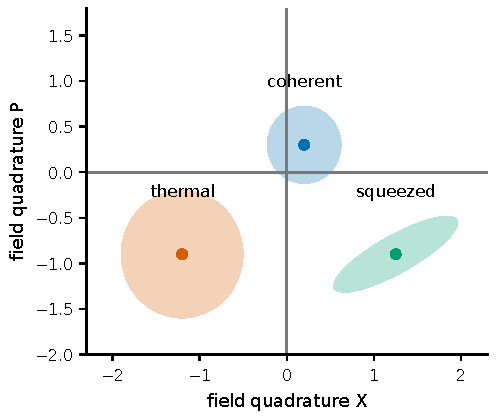
\includegraphics[width=0.72\linewidth]{figures/generated/chapter_03/ch03_phase_space_states.pdf}
\caption{相空间中三类常见单模光态的宽度。相干态的噪声接近真空圆斑，热态因随机强度和相位而变宽，压缩态把一个正交分量的涨落压低，同时把共轭分量的涨落抬高。}
\label{fig:ch03-phase-space}
\end{figure}

相空间图把一个模式写成两个正交分量 \(X\) 和 \(P\) 的概率图像。相干态像真空噪声大小的圆斑，只是圆心移动；热态仍近似圆形，但半径由 \(\bar n\) 放大；压缩态在一个方向变窄、另一个方向变宽。这个图像能帮助我们记住：不同光态的区别首先表现为涨落和相关，而不只是平均强度。

\section{为什么天体光通常要用密度矩阵和弱热光近似}

如果一个系统的所有自由度都被完整保留，可以用纯态描述。但天文观测几乎总是丢掉一些自由度：带外频率没记录，偏振可能没分辨，seeing 把空间模式混在一起，长时间 bin 把许多相干时间内的涨落加在一起。因此真正用于数据分析的状态通常是混合态。

相空间语言可以把这种混合写成不同表示。Glauber--Sudarshan \(P\) 表示把密度矩阵写成相干态混合，\(Q\) 函数对应异频探测时被真空噪声平滑后的分布：
\begin{equation}
  \rho=\int P(\alpha)|\alpha\rangle\langle\alpha|\,\mathrm{d}^2\alpha,
  \qquad
  Q(\alpha)=\frac{1}{\pi}\langle\alpha|\rho|\alpha\rangle .
  \label{eq:ch03-phase-space}
\end{equation}
\begin{formulaexplain}
\(\rho\) 是密度矩阵；\(P(\alpha)\) 是相干态混合权重；\(|\alpha\rangle\) 是相干态；\(Q(\alpha)\) 是由 \(\rho\) 投影得到的相空间分布。这个式子把“经典随机场”和“量子态”之间的边界写清楚。
\end{formulaexplain}
若 \(P(\alpha)\) 是正常的非负概率密度，许多强度和相干函数可以用经典随机场得到同样结果；热光和相干光在这个意义上常常是“经典”的。若 \(P\) 比 delta 函数还奇异，或 Wigner 函数出现负值，半经典图像就会失效。天体强度干涉的大部分基础公式处在半经典和量子理论等价的区域，但探测、损耗和弱光极限仍然更适合用密度矩阵记账 \citep{1963PhRvL..10..277S,1972PhRvA...6.2211A,2001qops.book.....S,1996PhRvL..76.4344B,1999PhRvA..60..674B}。

把未记录自由度丢掉的数学操作是 partial trace：
\begin{equation}
  \rho_{\rm obs}=\operatorname{Tr}_{\rm unobs}\rho_{\rm full}.
  \label{eq:ch03-partial-trace}
\end{equation}
\begin{formulaexplain}
\(\rho_{\rm full}\) 是包含所有自由度的完整状态；\(\operatorname{Tr}_{\rm unobs}\) 表示对未观测标签求迹；\(\rho_{\rm obs}\) 是数据实际保留的状态。它把“没有记录的信息要平均掉”写成密度矩阵操作。
\end{formulaexplain}
\(\rho_{\rm full}\) 可以包含源区位置、频率、传播路径、偏振、探测器内部自由度和环境；\(\rho_{\rm obs}\) 只保留数据中还可区分的自由度。这个公式说的不是抽象哲学，而是数据处理事实：没有记录的标签不能在似然函数里被当成可区分信息。宇宙学涨落退相干、引力透镜路径相干性限制和恒星强度干涉的视直径退相干，数学上都在处理“保留哪些自由度、平均掉哪些自由度”的问题 \citep{1998RvMP...70..101P,2020MNRAS.491.5789L,1996CQGra..13..377P}。

天体弱光极限还需要另一个数量级。热辐射的单模占有数由亮温 \(T_b\) 给出：
\begin{equation}
  \bar n_\nu=\frac{1}{\exp(h\nu/k_{\rm B}T_b)-1}.
  \label{eq:ch03-occupation}
\end{equation}
\begin{formulaexplain}
\(\bar n_\nu\) 是频率 \(\nu\) 的单模平均占有数；\(h\nu\) 是光子能量；\(k_{\rm B}T_b\) 是亮温对应的热能。它说明总光子率很高并不等于每个光学模式里有很多光子。
\end{formulaexplain}
\(h\nu\) 和 \(k_{\rm B}T_b\) 都是能量，单位 erg；\(\bar n_\nu\) 无量纲。式 \eqref{eq:ch03-occupation} 是单个玻色模式的 Bose--Einstein 占有数：光子数为 \(N\) 的能量为 \(Nh\nu\)，热权重按 \(\exp(-Nh\nu/k_{\rm B}T_b)\) 递减，归一化后得到几何分布；对这个分布求平均就得到 \(\bar n_\nu=[\exp(h\nu/k_{\rm B}T_b)-1]^{-1}\)。对 \(T_b=5800\,\mathrm{K}\) 的恒星表面，\(\lambda=500\,\mathrm{nm}\) 时 \(h\nu/k_{\rm B}T_b\simeq5\)，\(\bar n_\nu\simeq7\times10^{-3}\)；到 \(1\,\mu\mathrm{m}\) 时 \(\bar n_\nu\simeq0.09\)；到 \(10\,\mu\mathrm{m}\) 时可超过 1。射电和毫米波因为 \(h\nu\ll k_{\rm B}T_b\)，常进入高占有数、近经典波动的 Rayleigh--Jeans 区域。这个数量级解释了为什么光学天文可以有很高总光子率，却仍常处在每模式弱光极限。

\begin{figure}[tbp]
\centering
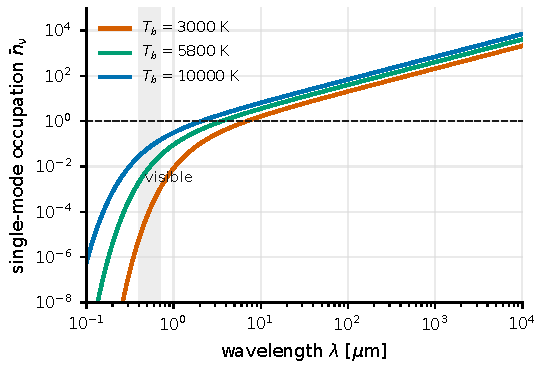
\includegraphics[width=0.82\linewidth]{figures/generated/chapter_03/ch03_blackbody_mode_occupation.pdf}
\caption{不同亮温黑体的单模占有数随波长变化。可见光灰带内，即使 \(T_b\) 为太阳量级，\(\bar n_\nu\) 也远小于 1；红外、毫米波或高亮温 maser 区域则可以进入 \(\bar n_\nu\gtrsim1\) 的强占有数极限。}
\label{fig:ch03-mode-occupation}
\end{figure}

在光学弱热光中，每个相干时间窗内常常没有光子，少数窗有一个光子。这个情况可写成
\begin{equation}
  \rho\simeq (1-\epsilon)\rho_0+\epsilon\rho_1+O(\epsilon^2),
  \qquad
  \epsilon\equiv\langle N\rangle_{\rm mode}\ll1.
  \label{eq:ch03-weak-thermal}
\end{equation}
\begin{formulaexplain}
\(\rho_0\) 是真空部分；\(\rho_1\) 是一光子部分；\(\epsilon\) 是单模式平均计数；\(O(\epsilon^2)\) 是双光子及更高项。弱热光极限下，大部分时间窗为空，少数点击携带空间和时间信息。
\end{formulaexplain}
\(\rho_0\) 是真空项，\(\rho_1\) 是一光子项，\(\epsilon\) 是该模式在该时间窗内的平均光子数。这个展开来自热态计数分布在 \(\bar n\ll1\) 时的最低阶：
\[
  P(0)=\frac{1}{1+\bar n}\simeq1-\bar n,
  \qquad
  P(1)=\frac{\bar n}{(1+\bar n)^2}\simeq\bar n,
  \qquad
  P(N\ge2)=O(\bar n^2).
\]
因此可以把 \(\epsilon\) 识别为单模式平均光子数。Tsang、Nair 和 Lu 的弱热光超分辨理论正是从这个展开出发：大多数相干时间窗没有点击，真正携带空间信息的是被探测到的一光子模式 \citep{1969JSP.....1..231H,2015Optic...2..646T,2016PhRvX...6c1033T}。这和天文事件表很吻合：零光子时间窗通常不会存入文件，留下来的是带时间戳的点击。

\section{光态怎样进入探测语言}

光场状态只有通过探测器才变成数据。理想光电探测器通过吸收光子产生点击，所以点击概率由场中的湮灭算符和产生算符按吸收事件的顺序组合而成。这个顺序通常叫正规序，它自动去掉“同一个光子和自己配对”的假项，因此单模二阶计数会出现 \(\langle \hat n(\hat n-1)\rangle\)，而不是普通的 \(\langle \hat n^2\rangle\)。

正规序给出的单模关系与 \(b_2\) 的定义一致。若只看一个模式，正频率场与湮灭算符成正比，\(\hat E^{(+)}\propto\hat a\)。一次点击对应一个吸收事件，两个点击对应两个吸收事件；于是平均计数与 \(\langle\hat a^\dagger\hat a\rangle=\langle\hat n\rangle\) 成正比，成对计数与 \(\langle\hat a^\dagger\hat a^\dagger\hat a\hat a\rangle=\langle\hat n(\hat n-1)\rangle\) 成正比。多通道、有限时间响应、背景和死时间会改变观测到的相关峰形和归一化，但不会改变“两个点击对应两个吸收事件”这个基本计数规则 \citep{1963PhRv..130.2529G,1965RvMP...37..231M,1995ocqo.book.....M,2017MNRAS.472.4126G}。

\section{非经典边界和天体 maser}

天体光能否表现出真正非经典统计？对单模式计数，最简单的边界是 \(b_2<1\)：同时探测两个光子的概率低于 Poisson 光，不能用正的经典强度涨落解释。实验室里的共振荧光和单光子源可以清楚地产生反聚束；天体观测却要面对多源混合、传播模式混合、背景和暗计数。即使某个微观过程发出非经典光，只要观测时无法隔离单个发射体和单个模式，最后的观测成对统计往往会被拉回 Poisson 基线 \citep{1977PhRvL..39..691K,1979OptL....4..205M,1995ocqo.book.....M}。

\begin{figure}[tbp]
\centering
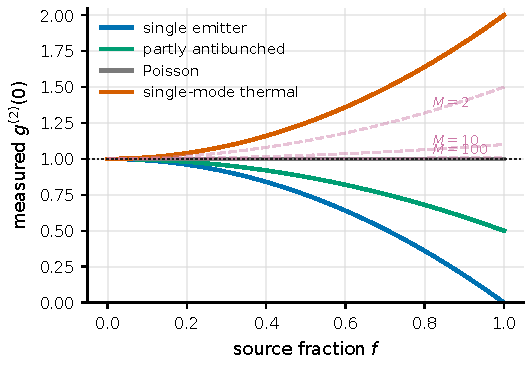
\includegraphics[width=0.74\linewidth]{figures/generated/chapter_03/ch03_nonclassical_mixing_boundary.pdf}
\caption{背景和多源混合会把观测到的成对统计拉向 Poisson 基线。蓝线表示理想单发射体反聚束，橙线表示单模热光聚束；源光子比例 \(f\) 下降时，偏离 1 的幅度按 \(f^2\) 变小。虚线显示多模热光 \(M>1\) 的聚束峰也会随模式数增大而变浅。}
\label{fig:ch03-nonclassical-mixing}
\end{figure}

受激辐射、maser 和 astrophysical laser 是容易被误说的边界情况。受激辐射可以给很高亮温和很窄线宽，射电 maser 的单模占有数可以非常大；但高亮温不等于相干态，窄线也不自动给 Poisson 成对统计。未饱和 maser、饱和 maser、多个斑点叠加、速度梯度和泵浦噪声会产生不同时间统计。若要用 photon correlation spectroscopy 区分自然 laser 成分，必须同时给出线宽、空间相干、偏振、背景连续谱和仪器时间响应，不能只凭“非 Poisson”判断新物理 \citep{1972ApJ...174..517G,2005NewA...10..361J,2008AIPC..984..216D,2017MNRAS.472.4126G}。

\begin{longtable}{p{0.16\linewidth}p{0.22\linewidth}p{0.20\linewidth}p{0.25\linewidth}}
\toprule
光态 & 单模计数 & \(b_2\) & 天文语境 \\
\midrule
数态 \(|n\rangle\) & 固定 \(N=n\) & \(1-1/n\) & 单发射体或量子源的理想模型，天体上极难隔离。 \\
相干态 & Poisson & 1 & 稳定激光的近似；天体窄线不必然是相干态。 \\
热态 & Bose--Einstein & 2 & 恒星连续谱和许多非相干源的基本模型；多模和仪器响应会降低观测对比度。 \\
压缩态 & 取决于测量正交量 & 可大于、小于或接近 1 & 仪器量子噪声工程重要，普通天体光不默认具有压缩。 \\
\bottomrule
\end{longtable}

\chapter{光子统计与相干函数}
\label{chap:04}

\begin{chapteropening}
前几章已经把光看成一串带标签的探测事件。现在要问的不是“平均有多亮”，而是“这些事件之间有没有关系”。如果两个时间门、两个探测器、两个频率通道或两个偏振通道里的光子只是各自随机到来，那么任何符合计数都只是偶然重合。如果它们比随机情形更常一起出现，或更少一起出现，事件表里就留下了光场统计的痕迹。Hanbury Brown--Twiss 实验、Glauber 相干理论和 Mandel 光子计数理论共同建立的，正是这套把事件表翻译成相干函数的语言 \citep{1956Natur.177...27B,1957RSPSA.242..300B,1958RSPSA.248..222B,1961AmJPh..29..539F,1963PhRv..130.2529G,1963PhRv..131.2766G,1965RvMP...37..231M,1995ocqo.book.....M,2000stop.book.....G,2007itcp.book.....W}。
\end{chapteropening}

\section{为什么先数事件对}

望远镜最后给出的不是一个抽象的“光场”，而是一张事件表。对第 \(j\) 个探测通道，可以写成
\[
  \mathcal{D}_j=\{t_{j,q},\nu_{j,q},p_{j,q},w_{j,q}\}_{q=1}^{N_j}.
\]
这里 \(t_{j,q}\) 是第 \(q\) 个事件的到达时间，通常用秒表示；\(\nu_{j,q}\) 是它落入的频率或波段；\(p_{j,q}\) 是偏振、探测器或电子通道标签；\(w_{j,q}\) 是质量权重，例如背景概率、坏像素掩膜或死时间修正。光学 HBT 与强度干涉常要处理 ns 量级的电子响应；X 射线和伽马射线事件表可能有 \(\mu{\rm s}\) 到 ms 的时间戳；普通成像和低时间分辨光谱若只保存积分后的像素强度，就已经把许多光子之间的时间关系平均掉了。

把连续时间切成宽度为 \(\Delta t\) 的小门，第 \(k\) 个时间门中的计数为
\begin{equation}
  N_{j,k}(\Delta t)=\sum_q w_{j,q}\,
  \mathbf{1}\!\left(t_k\leq t_{j,q}<t_k+\Delta t\right),
  \qquad
  \widehat r_{j,k}=\frac{N_{j,k}}{\Delta t}.
  \label{eq:ch04-count-bin}
\end{equation}
\begin{formulaexplain}
\(N_{j,k}\) 是通道 \(j\) 在第 \(k\) 个时间门内的计数；\(w_{j,q}\) 是事件权重；\(\mathbf 1(\cdots)\) 选择落入门内的事件；\(\widehat r_{j,k}\) 是该门的估计计数率。它把事件表变成可相关的时间序列。
\end{formulaexplain}
\(N_{j,k}\) 是无量纲计数，\(\widehat r_{j,k}\) 的单位是 \({\rm s^{-1}}\)。如果 \(\Delta t=1\,{\rm ns}\)，平均光子率为 \(10^6\,{\rm s^{-1}}\)，那么一个时间门内的平均计数只有 \(10^{-3}\)。也就是说，绝大多数 bin 是 0，少数 bin 是 1，同一个 bin 里有两个光子的概率很小。强度相关因此不是从一条肉眼可见的“光变曲线起伏”读出来的，而是从 \(10^8\) 到 \(10^{12}\) 个时间门或事件对的微小 excess 里累加出来的。

这立刻解释了为什么二阶计数理论里出现的是阶乘矩，而不是普通二阶矩：
\begin{equation}
  \left\langle N(N-1)\right\rangle.
  \label{eq:ch04-factorial-moment}
\end{equation}
\begin{formulaexplain}
\(N\) 是一个时间门内的光子数；\(N(N-1)\) 是不同光子组成的有序事件对数；尖括号表示统计平均。它比 \(N^2\) 少掉同一个光子和自己配对的假项。
\end{formulaexplain}
若一个时间门里有 \(N\) 个光子，可以组成 \(N^2\) 个“带顺序的选择”，但其中有 \(N\) 个是同一个光子和自己配对。符合探测不允许这样的自配对。一个 START 脉冲和一个 STOP 脉冲必须来自两个探测事件，因此可用的有序光子对数是 \(N(N-1)\)。这就是正规序算符在光电探测理论中的物理含义：探测器数的是不同的吸收事件，不是同一个事件的平方。Glauber 的相干函数把这一点写进算符次序，Mandel 的计数理论把它写进计数分布 \citep{1963PhRv..130.2529G,1963PhRv..131.2766G,1965RvMP...37..231M}。

\begin{figure}[tbp]
\centering
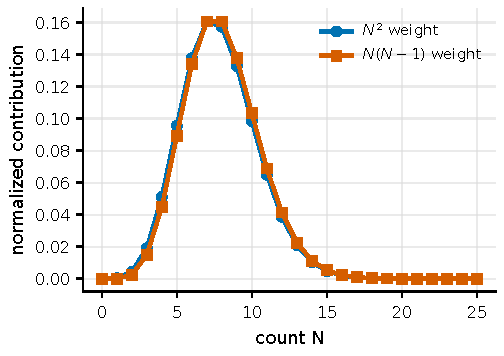
\includegraphics[width=0.86\linewidth]{figures/generated/chapter_04/ch04_factorial_moments.pdf}
\caption{Poisson 计数分布中，普通二阶矩 \(N^2\) 和阶乘矩 \(N(N-1)\) 对不同 \(N\) 的权重不同。符合探测只关心不同光子组成的光子对，因此 \(N(N-1)\) 自动去掉了同一光子的自配对项。}
\label{fig:ch04-factorial-moments}
\end{figure}

事件对还必须和仪器效应分开。单光子探测器在一次触发后通常有一段不能再次响应的死时间。APD、PMT 或 SiPM 的死时间可以是 \(10\)--\(100\,{\rm ns}\)，而可见光热光的相干时间常在 ps 或更短。若直接在同一个探测器上做自相关，零延迟附近会被死时间挖出一个仪器空洞；afterpulsing 又可能在非零延迟制造假峰。因此许多零延迟光子统计实验会先用分束器把同一束光分到两个独立探测器，再做交叉相关。Guerin 等人的恒星热光聚束实验就是这种结构：1 m 望远镜、多模光纤、分束器、两只 APD 和 TDC 延迟直方图。他们的 APD 死时间约 \(22\,{\rm ns}\)，而光学相干时间只有 ps 量级；若不分束，天体的聚束峰会和探测器恢复时间纠缠在一起 \citep{2017MNRAS.472.4126G}。

\begin{figure}[tbp]
\centering
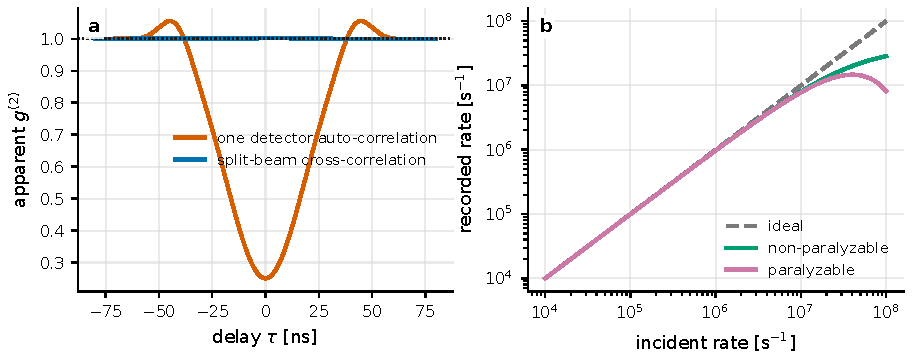
\includegraphics[width=0.92\linewidth]{figures/generated/chapter_04/ch04_deadtime_pileup_bias.pdf}
\caption{死时间、pile-up 和 afterpulsing 对短延迟相关的影响。左图显示单探测器自相关会出现零延迟空洞和非零延迟假峰，分束后的双探测器交叉相关更接近真实热光聚束峰；右图显示入射光子率升高后，不同死时间模型会给出不同的记录率饱和曲线。}
\label{fig:ch04-deadtime-pileup}
\end{figure}

\begin{longtable}{p{0.20\linewidth}p{0.25\linewidth}p{0.42\linewidth}}
\toprule
量 & 单位和典型范围 & 物理意义 \\
\midrule
\(t_{j,q}\) & s；精度从 ns 到 ms & 单个探测事件的到达时间；相关函数的横轴由事件时间差构成。 \\
\(\Delta t\) & ps 到 s & 人为选择的计数门宽或电子采样间隔；若远大于相干时间，会稀释聚束峰。 \\
\(r_j\) & \({\rm s^{-1}}\)；光学 HBT 常 \(10^5\)--\(10^7\) & 第 \(j\) 个通道的平均计数率，决定 shot noise 和可用事件对数。 \\
\(\tau_d\) & ns 到 \(\mu{\rm s}\) & 探测器死时间；若和待测延迟相近，需要用分束、交叉相关或死时间模型修正。 \\
\(H_{AB}(\tau)\) & 每个延迟 bin 的计数 & 两通道事件对的延迟直方图；归一化后给出 \(g^{(2)}\)。 \\
\bottomrule
\end{longtable}

\section{一阶和二阶相干到底在问什么}

相干函数看起来像形式化定义，但每一阶都对应一个很朴素的问题。一阶相干问：“同一束光在两个时刻的电场振幅和相位是否还相互记得？”二阶相干问：“两个强度探测事件是否比随机情形更容易成对出现？”前一个问题属于电场相位记忆，后一个问题属于光子到达的联合概率。振幅干涉主要利用前者，强度干涉和 HBT 主要利用后者。

在探测面上，把正频率电场算符写作 \(\hat E^{(+)}(t)\)，负频率部分写作 \(\hat E^{(-)}(t)\)。一阶相干函数定义为
\begin{equation}
  G^{(1)}(t_1,t_2)
  =
  \left\langle
    \hat E^{(-)}(t_1)\hat E^{(+)}(t_2)
  \right\rangle,
  \qquad
  g^{(1)}(\tau)=\frac{G^{(1)}(t,t+\tau)}{G^{(1)}(t,t)} .
  \label{eq:ch04-g1}
\end{equation}
\begin{formulaexplain}
\(G^{(1)}\) 是一阶场相关函数；\(\hat E^{(+)}\)、\(\hat E^{(-)}\) 是正、负频率场算符；\(g^{(1)}\) 是归一化结果；\(\tau\) 是时间延迟。它测的是电场相位和振幅隔一段时间后还保留多少记忆。
\end{formulaexplain}
\(G^{(1)}\) 带有强度单位，归一化后的 \(g^{(1)}\) 无量纲。若光场平稳，相关只依赖延迟 \(\tau=t_2-t_1\)。当 \(|g^{(1)}(\tau)|\) 接近 1 时，延迟 \(\tau\) 后的电场仍能和原来的电场形成清晰干涉；当它接近 0 时，相位已经基本失去记忆。振幅干涉仪测到的条纹可见度，正是空间版本的 \(g^{(1)}\)。

光谱带宽决定了这种相位记忆能维持多久。若滤光片中心波长为 \(\lambda\)，带宽为 \(\Delta\lambda\ll\lambda\)，频率带宽近似为
\begin{equation}
  \Delta\nu \simeq \frac{c\,\Delta\lambda}{\lambda^2},
  \qquad
  \tau_c \sim \frac{1}{\Delta\nu}
  \simeq \frac{\lambda^2}{c\,\Delta\lambda}.
  \label{eq:ch04-coherence-time}
\end{equation}
\begin{formulaexplain}
\(\Delta\nu\) 是频率带宽；\(\Delta\lambda\) 是波长带宽；\(\lambda\) 是中心波长；\(c\) 是光速；\(\tau_c\) 是相干时间。这个式子把滤光片带宽直接换成热光相关峰的时间尺度。
\end{formulaexplain}
\(\tau_c\) 是相干时间，单位是秒。它不是探测器时间分辨率，而是光本身由带宽决定的相位记忆时间。例如 \(\lambda=780\,{\rm nm}\)、\(\Delta\lambda=1\,{\rm nm}\) 时，\(\tau_c\) 约为 \(2\,{\rm ps}\)。普通可见光宽带滤光片给出的热光相干时间通常远短于 ns 电子响应。这个数量级会在恒星聚束实验、窄线 photon-correlation spectroscopy 和第 \ref{chap:05} 章的空间强度干涉中反复出现 \citep{2008AIPC..984..216D,2009A&A...507.1719F,2017MNRAS.472.4126G}。

\Needspace{13\baselineskip}
二阶相干函数把问题从“电场是否还记得相位”改成“两个探测事件是否相关”。量子探测理论给出的定义是
\begin{equation}
  G^{(2)}(t_1,t_2)
  =
  \left\langle
    \hat E^{(-)}(t_1)\hat E^{(-)}(t_2)
    \hat E^{(+)}(t_2)\hat E^{(+)}(t_1)
  \right\rangle,
  \qquad
  g^{(2)}(\tau)=
  \frac{G^{(2)}(t,t+\tau)}
  {G^{(1)}(t,t)\,G^{(1)}(t+\tau,t+\tau)} .
  \label{eq:ch04-g2}
\end{equation}
\begin{formulaexplain}
\(G^{(2)}\) 是二阶正规序场相关；分子数共同探测，分母给随机符合基线；\(g^{(2)}\) 是归一化结果。它测的是光子是否倾向于成对到达。
\end{formulaexplain}
这个式子可以逐项读。右端分母是两个时刻各自的平均强度，代表“若两个探测完全独立，随机符合数应该是多少”。分子是两个探测事件共同发生的强度相关。归一化以后，\(g^{(2)}\) 无量纲。独立 Poisson 到达给 \(g^{(2)}=1\)；若 \(g^{(2)}(0)>1\)，零延迟附近的光子对比随机情形更多，称为聚束；理想单一时空偏振模式的热光给 \(g^{(2)}(0)=2\)。若 \(g^{(2)}(0)<1\)，零延迟符合被压低，称为反聚束；这不能由正定经典强度涨落解释，是单光子源和共振荧光的标准量子光学判据 \citep{1977PhRvL..39..691K,1979OptL....4..205M,1986PhRvA..33.4033Y,1993PhRvL..71.4287Z,2005Natur.436...87B}。

在工程估算中，人们常把同一个定义写成连续强度形式
\begin{equation}
  g^{(2)}(\tau)=
  \frac{\left\langle I(t)I(t+\tau)\right\rangle}
       {\left\langle I(t)\right\rangle^2}
  \label{eq:ch04-classical-g2}
\end{equation}
\begin{formulaexplain}
\(I(t)\) 是强度或探测电流；\(\tau\) 是延迟；分子是强度共同涨落；分母是平均强度平方。这个经典写法适合工程估算，但必须说明 \(I(t)\) 是否已被探测器响应卷积。
\end{formulaexplain}
但这行式子要谨慎使用。这里的 \(I(t)\) 可以是理想瞬时强度，也可以是探测器输出电流、TDC 事件率或采样后的 ADC 值。若 \(I(t)\) 已经被 \(4\,{\rm ns}\) 电子响应卷积，式中得到的是响应后的 \(g^{(2)}\)，不是光场本身 ps 宽度的相关峰。许多天文强度相关信号并不是“没有聚束”，而是聚束峰被有限时间响应、多个模式和背景光压低到 \(10^{-3}\)、\(10^{-6}\) 甚至更小。

\section{计数分布怎样进入相关估计}

单模成对因子 \(b_2\) 在事件表中表现为固定时间门计数的阶乘矩。只看平均光子率不够，因为不同光场可以有相同的平均亮度，却有完全不同的计数起伏。把一个固定时间门里的计数记为 \(N\)，均值为 \(\bar{N}\)，方差为 \(\sigma_N^2\)。Mandel 参数定义为
\begin{equation}
  Q=\frac{\sigma_N^2-\bar{N}}{\bar{N}}.
  \label{eq:ch04-mandel-q}
\end{equation}
\begin{formulaexplain}
\(Q\) 是 Mandel 参数；\(\sigma_N^2\) 是时间门计数方差；\(\bar N\) 是平均计数。它用 Poisson 方差 \(\sigma_N^2=\bar N\) 作零点，区分超 Poisson、Poisson 和亚 Poisson 统计。
\end{formulaexplain}
这个定义把 Poisson shot noise 当作零点。\(Q=0\) 表示方差正好等于均值；\(Q>0\) 表示超 Poisson 起伏，常见于热光或强度涨落很大的混沌光；\(Q<0\) 表示亚 Poisson 起伏，意味着计数比 Poisson 更规整，是非经典统计的重要信号。

\(Q\) 和零延迟二阶相干的联系来自一个简单代数恒等式：
\[
  \left\langle N(N-1)\right\rangle
  =
  \left\langle N^2\right\rangle-\bar{N}
  =
  \sigma_N^2+\bar{N}^2-\bar{N}.
\]
因此
\begin{equation}
  g^{(2)}(0)=
  \frac{\left\langle N(N-1)\right\rangle}{\bar{N}^2}
  =
  1+\frac{Q}{\bar{N}}.
  \label{eq:ch04-q-g2}
\end{equation}
\begin{formulaexplain}
\(g^{(2)}(0)\) 是零延迟二阶相干；\(\langle N(N-1)\rangle\) 是阶乘矩；\(\bar N\) 是平均门计数；\(Q\) 是 Mandel 参数。它把计数方差语言和光子成对到达语言连起来。
\end{formulaexplain}
这里的 \(N\) 是一个时间门内的计数，不是整晚观测的总计数。若把时间门加宽，\(\bar{N}\) 增大，许多彼此不相干的时间模式会被平均进同一个 \(N\)，于是同一内禀光场的 \(g^{(2)}(0)-1\) 会被稀释。这个式子也是一个提醒：不能只报 \(Q\) 或只报 \(g^{(2)}(0)\)，还要说明时间门宽、模式数和平均计数。

\begin{figure}[tbp]
\centering
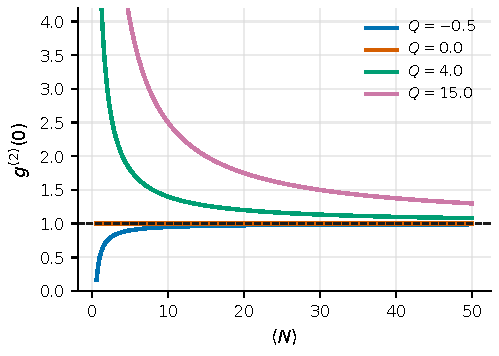
\includegraphics[width=0.86\linewidth]{figures/generated/chapter_04/ch04_mandel_q_g2.pdf}
\caption{在固定时间门内，Mandel \(Q\) 通过 \(g^{(2)}(0)=1+Q/\langle N\rangle\) 改变零延迟二阶相干。低平均计数时，同样的 \(Q\) 会造成更大的 \(g^{(2)}(0)\) 偏离；平均许多模式后，曲线逐渐回到 1。}
\label{fig:ch04-mandel-q-g2}
\end{figure}

\Needspace{10\baselineskip}
单模热态在时间门计数语言中写成 Bose--Einstein 分布：
\begin{equation}
  P(N)=\frac{\bar{N}^{\,N}}{(1+\bar{N})^{N+1}},
  \qquad
  \sigma_N^2=\bar{N}+\bar{N}^2,
  \qquad
  g^{(2)}(0)=2.
  \label{eq:ch04-thermal-count}
\end{equation}
\begin{formulaexplain}
\(P(N)\) 是单模热光计数概率；\(\bar N\) 是该时间门内的平均计数；\(\sigma_N^2\) 是方差；\(g^{(2)}(0)=2\) 是理想聚束峰。它把热态光子数统计改写成可用于事件表的形式。
\end{formulaexplain}
方差里的 \(\bar{N}\) 是 shot noise，\(\bar{N}^2\) 是热光的波动噪声。物理图像是这样的：热光的电场由许多随机相位的微小贡献叠加，瞬时强度会形成随机明暗起伏；探测器在亮斑时更容易接连记录多个光子，于是零延迟附近的符合计数升高。这就是 HBT 聚束。

真实望远镜通常不会只收一个单一模式。若 \(M\) 个强度相近且相互独立的热光模式被同一个探测器平均，方差和聚束峰变成
\begin{equation}
  \sigma_N^2=\bar{N}+\frac{\bar{N}^2}{M},
  \qquad
  g^{(2)}(0)=1+\frac{1}{M}.
  \label{eq:ch04-multimode}
\end{equation}
\begin{formulaexplain}
\(M\) 是独立热光模式数；\(\bar N^2/M\) 是被多模平均后的额外波动噪声；\(g^{(2)}(0)-1=1/M\) 是聚束 excess。它解释了为什么天文多模数据里的峰高远小于 1。
\end{formulaexplain}
这里的 \(M\) 可以来自两个偏振、多个空间 speckle、宽光谱里的多个频率模式，也可以来自一个时间门内包含的多个相干时间。未分偏振的热光点源通常已经有 \(M_{\rm pol}\simeq2\)，理想峰高从 2 降到 1.5。若电子时间门比相干时间宽 \(10^3\) 倍，时间模式平均又会把 excess 再压低约 \(10^3\) 倍。这就是为什么天文 HBT 图上常看到的是 \(g^{(2)}-1\) 的小数，而不是教科书里的 1。

相干态在同样的时间门里给 Poisson 计数：
\begin{equation}
  P(N)=e^{-\bar{N}}\frac{\bar{N}^N}{N!},
  \qquad
  \sigma_N^2=\bar{N},
  \qquad
  g^{(2)}(\tau)=1.
  \label{eq:ch04-poisson-count}
\end{equation}
\begin{formulaexplain}
\(P(N)\) 是 Poisson 分布；\(\bar N\) 是平均计数；\(N!\) 归一化离散计数；\(\sigma_N^2=\bar N\) 是 shot noise；\(g^{(2)}=1\) 表示没有过量或不足的事件对。它是相干态在事件时间门中的写法。
\end{formulaexplain}
理想激光可以有很长的一阶相干时间，却没有热光式二阶聚束。因此“相干”一词在天文学里要分清含义：射电 maser、脉冲星相干曲率辐射、天体激光候选线和非热同步辐射，可能在一阶相干、二阶相干和多源平均上表现出不同统计。许多天体 maser 是大量小 coherence cell 的叠加，观测到的 \(g^{(2)}\) 不一定像实验室单模激光 \citep{1977ApJ...212..800C,1991ApJ...383..808M,2004A&A...428..497J,2005MNRAS.364..731J,2005NewA...10..361J,2008AIPC..984..216D,2009A&A...507.1719F}。

\section{Siegert 关系把 HBT 和场相干联系起来}

现在可以回到 HBT 的核心问题：为什么强度相关能告诉我们场相干信息？关键是热光或更一般的高斯混沌光有一个特殊性质。电场是许多独立小贡献的随机叠加时，复电场近似服从高斯统计；四阶矩可以拆成二阶矩的组合。用经典符号写，直观上就是
\[
  \left\langle I(t)I(t+\tau)\right\rangle
  =
  \left\langle I\right\rangle^2
  +
  \left|G^{(1)}(\tau)\right|^2
\]
再除以平均强度平方，就得到 Siegert 关系：
\begin{equation}
  g^{(2)}(\tau)=1+\zeta\left|g^{(1)}(\tau)\right|^2 .
  \label{eq:ch04-siegert}
\end{equation}
\begin{formulaexplain}
\(g^{(2)}-1\) 是强度相关 excess；\(g^{(1)}\) 是归一化一阶场相干；\(\zeta\) 是模式、偏振、背景和响应造成的可见度因子。它是 HBT 从强度相关读出场相干模平方的核心桥梁。
\end{formulaexplain}
\(\zeta\) 是可见度因子，满足 \(0<\zeta\leq1\)。理想单一时空偏振模式有 \(\zeta=1\)；未分偏振、多空间模式、有限带宽平均、背景光和仪器响应都会降低 \(\zeta\)。如果源光子只占两个通道总计数的比例分别为 \(f_A\) 和 \(f_B\)，且背景不相关也没有自己的聚束峰，那么相关峰幅度还要近似乘上 \(f_A f_B\)。

\begin{figure}[tbp]
\centering
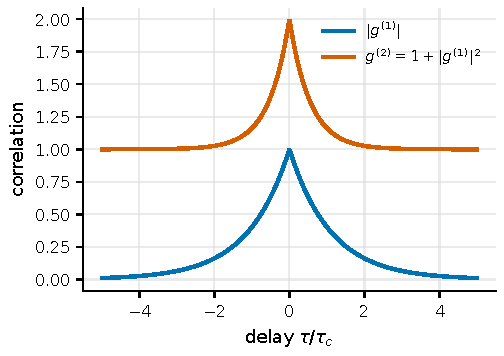
\includegraphics[width=0.86\linewidth]{figures/generated/chapter_04/ch04_siegert_relation.pdf}
\caption{热光的 Siegert 关系把一阶场相干的衰减转化为二阶强度聚束峰。若 \(|g^{(1)}|\) 随延迟以相干时间 \(\tau_c\) 衰减，\(g^{(2)}-1\) 以 \(|g^{(1)}|^2\) 衰减，并在大延迟回到无相关值 0。实际峰高还要乘以模式数、背景和时间响应因子。}
\label{fig:ch04-siegert}
\end{figure}

式 \eqref{eq:ch04-siegert} 的意义很大。左边是事件表可测的强度相关；右边的 \(g^{(1)}\) 是电场相干，可由光谱的傅里叶变换得到，也可由振幅干涉仪的可见度测得。若光谱近似矩形，\(|g^{(1)}(\tau)|^2\) 近似 \({\rm sinc}^2(\Delta\nu\tau)\)；若谱线近似 Lorentzian，\(|g^{(1)}|\) 是指数衰减；若谱线近似 Gaussian，\(|g^{(1)}|^2\) 也是 Gaussian。窄谱线 photon-correlation spectroscopy 正是利用 \(g^{(2)}(\tau)\) 的宽度反推谱线宽度。对于 \(\eta\) Carinae 附近的 Fe II 或 O I 天体激光候选线，普通光谱仪很难达到 \(R\sim10^8\) 的分辨率，而 ns 量级的强度相关可以对 MHz 到 GHz 线宽给出独立约束 \citep{2005NewA...10..361J,2008AIPC..984..216D,2014ApJ...789L..10T}。

Siegert 关系也是第 \ref{chap:05} 章空间强度干涉的入口。把时间延迟 \(\tau\) 换成两台望远镜之间的空间基线 \(\mathbf{B}\)，\(g^{(1)}\) 就变成天空亮度分布的复可见度，强度相关测到的 excess 与 \(|g^{(1)}|^2\) 成正比。也就是说，HBT 不需要把两台望远镜的电场直接合束，却仍能通过强度涨落的同步程度得到可见度模平方。这一结论成立的前提，就是源光近似热光或高斯混沌光，并且仪器归一化没有把背景、模式数和时间响应混在一起。

这些前提不能省略。理想相干态满足长程 \(g^{(1)}\)，但 \(g^{(2)}=1\)，因此不服从热光式 \(1+|g^{(1)}|^2\)。反聚束光、压缩光、单光子源、强烈非平稳脉冲和少数相干子源叠加都可能打破式 \eqref{eq:ch04-siegert}。实验室量子光学已经在许多体系里测到非经典 \(g^{(2)}\)；天文上更常见的情况是混合场，例如许多非热小源平均后近似热光，或热连续谱上叠加窄非热线 \citep{1965PhRv..140..676T,1977PhRvL..39..691K,1979OptL....4..205M,2000PhRvA..62d3816S,2008PhRvA..78f1802S,2012PhRvL.109n7404Z,2020MNRAS.491.5789L}。

\section{从理想相关到望远镜里的估计量}

真实探测器测到的不是无限窄时间响应下的 \(g_{\rm true}^{(2)}\)，而是它和仪器响应的卷积：
\begin{equation}
  g_{\rm obs}^{(2)}(\tau)-1 =
  \int_{-\infty}^{+\infty}
  \left[g_{\rm true}^{(2)}(\tau')-1\right]
  R_{\Delta t}(\tau-\tau')\,d\tau',
  \label{eq:ch04-response-convolution}
\end{equation}
\begin{formulaexplain}
\(g_{\rm true}^{(2)}\) 是光场本征相关；\(g_{\rm obs}^{(2)}\) 是观测相关；\(R_{\Delta t}\) 是归一化仪器响应函数；\(\tau'\) 是积分变量。这个卷积说明有限时间响应会拉宽并压低窄相关峰。
\end{formulaexplain}
其中 \(R_{\Delta t}\) 的面积归一化为 1，宽度由探测器 jitter、电子带宽、采样窗口和分析 bin 共同决定。这个式子说明了一个容易误解的事实：卷积主要守住相关峰的面积，却会把窄峰拉宽、压低。若内禀峰宽 \(\tau_c\) 远小于有效响应宽度 \(\Delta t_{\rm eff}\)，峰值近似按
\begin{equation}
  C_{\rm obs}\equiv g_{\rm obs}^{(2)}(0)-1
  \simeq
  C_{\rm true}\,
  \frac{\tau_c}{\Delta t_{\rm eff}}\,
  \frac{1}{M_{\rm pol}M_{\rm sp}}\,
  f_A f_B
  \label{eq:ch04-contrast-dilution}
\end{equation}
\begin{formulaexplain}
\(C_{\rm obs}\) 和 \(C_{\rm true}\) 是观测与理想峰高；\(\tau_c/\Delta t_{\rm eff}\) 是时间稀释；\(M_{\rm pol},M_{\rm sp}\) 是偏振和空间模式数；\(f_Af_B\) 是背景稀释。它是望远镜中相关峰幅度的误差预算式。
\end{formulaexplain}
被稀释。这里 \(C_{\rm true}\) 是理想峰高；\(M_{\rm pol}\) 和 \(M_{\rm sp}\) 是偏振和空间模式数；\(f_A,f_B\) 是两通道里源光子占总计数的比例。式 \eqref{eq:ch04-contrast-dilution} 是数量级公式。精确分析应把实测响应函数、光谱给出的 \(|g^{(1)}|^2\)、背景和电子学相关一起放进模型。

\begin{figure}[tbp]
\centering
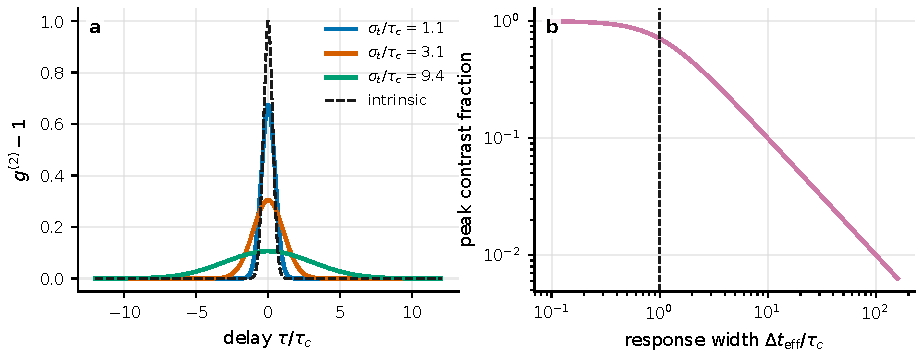
\includegraphics[width=0.95\linewidth]{figures/generated/chapter_04/ch04_response_convolution.pdf}
\caption{有限时间响应会把窄的热光聚束峰拉宽并压低。左图中虚线是内禀 ps 量级峰，实线是不同响应宽度卷积后的观测峰；右图显示当 \(\Delta t_{\rm eff}\gg\tau_c\) 时，零延迟峰高近似按 \(\tau_c/\Delta t_{\rm eff}\) 下降。}
\label{fig:ch04-response-convolution}
\end{figure}

Guerin 等人的恒星聚束实验给出了一组有用的标尺。中心波长约 \(7800\,\text{\AA}\)，最窄滤光片宽度 \(10\,\text{\AA}\)，对应 \(\Delta\nu\simeq5\times10^{11}\,{\rm Hz}\) 和 \(\tau_c\simeq1.6\)--\(2\,{\rm ps}\)。APD 的单光子时间 jitter 约 \(500\,{\rm ps}\)，两个探测器的相对响应峰宽约 \(700\,{\rm ps}\)。理想热光 \(C_{\rm true}=1\)，但卷积后预期观测峰只有 \(C_{\rm obs}\simeq2.2\times10^{-3}\)；实验室热源测到 \((2.01\pm0.09)\times10^{-3}\)，三颗亮星也给出约 \(1.8\)--\(2.0\times10^{-3}\) 的峰 \citep{2017MNRAS.472.4126G}。因此望远镜相关图上直接出现的通常不是 \(g^{(2)}(0)=2\)，而是 \(1+10^{-3}\)、\(1+10^{-6}\) 或更小的 excess。

事件表里的交叉相关估计量可以写成延迟直方图。对两个通道 \(A,B\)，bin 宽为 \(\delta\tau\)，总 live time 为 \(T\)，
\begin{equation}
  H_{AB}(\tau_m)
  =
  \sum_{i\in A}\sum_{j\in B}
  \mathbf{1}\!\left(
    \tau_m-\frac{\delta\tau}{2}
    \leq t_{B,j}-t_{A,i}
    < \tau_m+\frac{\delta\tau}{2}
  \right),
  \label{eq:ch04-delay-histogram}
\end{equation}
\begin{formulaexplain}
\(H_{AB}(\tau_m)\) 是通道 \(A,B\) 的事件对延迟直方图；\(t_{B,j}-t_{A,i}\) 是一对事件的延迟；\(\tau_m\) 是延迟 bin 中心；\(\delta\tau\) 是 bin 宽。它把事件表直接变成相关函数的原始计数。
\end{formulaexplain}
\begin{equation}
  \widehat g^{(2)}_{AB}(\tau_m)
  =
  \frac{H_{AB}(\tau_m)}
  {r_A r_B\,\delta\tau\,T}.
  \label{eq:ch04-g2-estimator}
\end{equation}
\begin{formulaexplain}
\(\widehat g^{(2)}_{AB}\) 是二阶相关估计量；\(r_A,r_B\) 是两通道平均计数率；\(\delta\tau T\) 给出延迟 bin 和 live time；分母是随机符合期望。它把直方图归一化到“无相关时等于 1”的尺度。
\end{formulaexplain}
\(H_{AB}\) 是观测到的事件对数；分母是同样 live time、同样 bin 宽、同样平均计数率下的随机符合期望，所以 \(\widehat g^{(2)}\) 无量纲。真实分析常不用解析分母，而用大时间偏移、不同观测段、偏振错配或 off-source 通道构造参考直方图 \(H_{\rm ref}(\tau)\)，再取比值或差值。这样可以吸收 TDC bin 宽不均、电子串扰、慢变透明度和采样窗口边缘效应。

\begin{figure}[tbp]
\centering
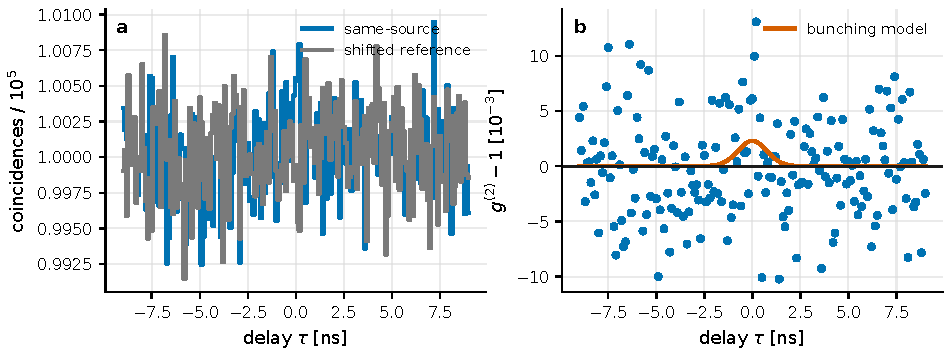
\includegraphics[width=0.95\linewidth]{figures/generated/chapter_04/ch04_delay_histogram_estimator.pdf}
\caption{延迟直方图估计量的结构。左图中同源事件对直方图在零延迟附近比移位参考直方图多出很小的符合数；右图把差值按随机符合数归一化后得到 \(g^{(2)}-1\)，峰值只有 \(10^{-3}\) 量级。真实观测还要加入死时间、背景和响应函数修正。}
\label{fig:ch04-delay-histogram}
\end{figure}

误差主要来自随机符合对数。若某个延迟 bin 中随机符合数为 \(N_{\rm pair}\)，shot-noise 误差的数量级是
\begin{equation}
  \sigma\!\left[\widehat g^{(2)}(\tau)\right]\sim N_{\rm pair}^{-1/2}.
  \label{eq:ch04-shot-noise}
\end{equation}
\begin{formulaexplain}
\(\sigma[\widehat g^{(2)}]\) 是相关估计量的统计误差；\(N_{\rm pair}\) 是该延迟 bin 中的随机符合对数。它说明强度相关的精度主要靠积累大量独立事件对。
\end{formulaexplain}
以两个 \(10^6\,{\rm s^{-1}}\) 通道、\(\delta\tau=100\,{\rm ps}\)、\(T=1\,{\rm hr}\) 为例，随机符合数约 \(3.6\times10^8\)，单 bin 统计误差约 \(5\times10^{-5}\)。如果聚束峰跨越多个 bin，可以拟合整个峰而不只看零延迟 bin；如果系统相关停在 \(10^{-3}\) 量级，继续增加曝光也不会替代 TDC、电子串扰和背景归一化修正。Guerin 等人的数据在修正 TDC spurious correlation 后接近 \(N^{-1/2}\) 标度；现代 VERITAS 和 MAGIC 系统则通过离线相关、GPU/FPGA 相关器和许多基线平均，把同一思想推广到空间强度干涉 \citep{2017MNRAS.472.4126G,2020NatAs...4.1164A,2024MNRAS.529.4387A}。

\Needspace{14\baselineskip}
二阶相关只用光子对。若同时保留三个望远镜或三个时间通道，可以定义三阶强度相关
\begin{equation}
  g^{(3)}_{123}=
  \frac{\left\langle I_1 I_2 I_3\right\rangle}
       {\left\langle I_1\right\rangle
        \left\langle I_2\right\rangle
        \left\langle I_3\right\rangle}.
  \label{eq:ch04-g3}
\end{equation}
\begin{formulaexplain}
\(g^{(3)}_{123}\) 是三通道归一化强度相关；\(I_1,I_2,I_3\) 是三个望远镜或时间通道的强度；分母给随机三重符合基线。它把统计对象从光子对推广到光子三元组。
\end{formulaexplain}
对于高斯混沌光，三阶相关包含三个二阶项和一个闭合三角形项：
\begin{equation}
  g^{(3)}_{123}
  =
  1
  +|\gamma_{12}|^2+|\gamma_{23}|^2+|\gamma_{31}|^2
  +2\,{\rm Re}\!\left(\gamma_{12}\gamma_{23}\gamma_{31}\right).
  \label{eq:ch04-g3-closure}
\end{equation}
\begin{formulaexplain}
\(\gamma_{ij}\) 是通道 \(i,j\) 的一阶相干度；模平方项来自三条基线；\({\rm Re}(\gamma_{12}\gamma_{23}\gamma_{31})\) 是闭合三角形项。它是三阶强度干涉恢复相位组合的入口。
\end{formulaexplain}
\(\gamma_{ij}\) 是第 \(i,j\) 个通道之间的一阶相干度。最后一项包含闭合相位，因此三阶强度相关原则上能把第 \ref{chap:05} 章中丢失的 Fourier 相位组合找回来。代价是噪声更大：光子三元组比光子对少得多，对系统误差也更敏感。Gamo 的早期理论、Ofir--Ribak 思路、Nuñez 等人的成像模拟和 CTA 相关研究都把高阶相关视作强度干涉成像的重要延伸 \citep{1966JOSA...56..441G,2012MNRAS.419..172N,2012MNRAS.424.1006N,2013APh....43..331D,2014SPIE.9146E..0ZD}。

\begin{figure}[tbp]
\centering
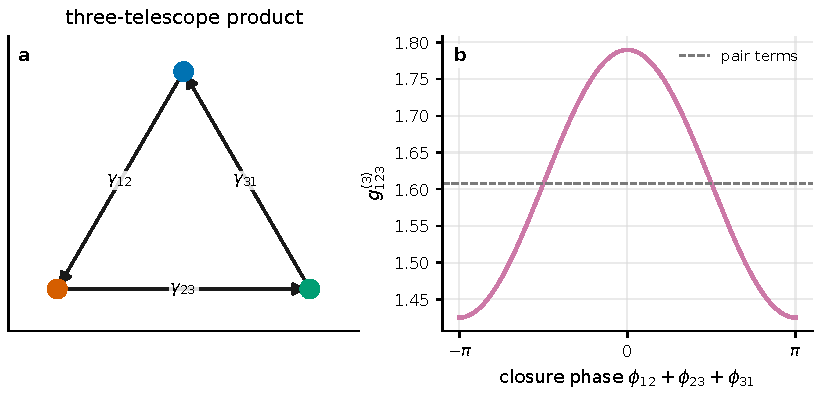
\includegraphics[width=0.92\linewidth]{figures/generated/chapter_04/ch04_g3_closure_phase.pdf}
\caption{三阶强度相关中闭合相位项的来源。左图中三台望远镜形成 \(\gamma_{12}\gamma_{23}\gamma_{31}\) 的闭合乘积；右图显示在固定 \(|\gamma_{ij}|\) 下，\(g^{(3)}\) 会随闭合相位余弦变化。二阶强度干涉只给 \(|\gamma|^2\)，三阶项才开始对相位组合敏感。}
\label{fig:ch04-g3-closure}
\end{figure}

频率分辨和偏振分辨的二阶相关写作
\begin{equation}
  g^{(2)}_{pq}(\nu_1,\nu_2,\tau)=
  \frac{
    \left\langle I_p(\nu_1,t)I_q(\nu_2,t+\tau)\right\rangle
  }{
    \left\langle I_p(\nu_1,t)\right\rangle
    \left\langle I_q(\nu_2,t)\right\rangle
  } .
  \label{eq:ch04-frequency-polarization-g2}
\end{equation}
\begin{formulaexplain}
\(p,q\) 是偏振通道；\(\nu_1,\nu_2\) 是两个频率通道；\(\tau\) 是时间延迟；分子是跨频率、跨偏振的强度共同涨落。它把二阶相关推广成可分析谱线、连续谱和偏振耦合的通道矩阵。
\end{formulaexplain}
\(p,q\) 是偏振通道，\(\nu_1,\nu_2\) 是频率或窄带滤光片中心。若两个频率采样同一条热谱线内的相干宽度，它们的强度涨落可以相关；若相隔远大于线宽，相关应回到 1。若两个偏振来自同一物理辐射过程，交叉偏振相关可能探测磁场几何或散射几何；若偏振通道混合了独立模式，聚束峰会被平均掉。对快速瞬变、脉冲星、FRB 光学对应体、天体 maser/laser 候选线和极端高时间分辨观测，保留事件级频率和偏振标签比只保存一条总光变曲线更有价值 \citep{2009A&A...507.1719F,2014ApJ...789L..10T,2024arXiv240418606N}。

\begin{figure}[tbp]
\centering
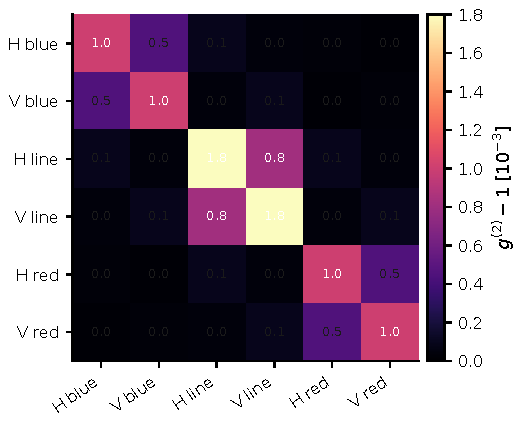
\includegraphics[width=0.72\linewidth]{figures/generated/chapter_04/ch04_frequency_polarization_matrix.pdf}
\caption{频率和偏振分辨 \(g^{(2)}\) 可以写成跨通道矩阵。谱线通道因为相干时间较长而有较高 excess，同一偏振通道的相关通常强于正交偏振通道；矩阵中的非对角元给出跨频率、跨偏振的共同涨落。}
\label{fig:ch04-frequency-polarization}
\end{figure}

\part[仪器、强度干涉和信息极限]{仪器、强度干涉和信息极限}
\chapter{空间相干与强度干涉}
\label{chap:05}

\begin{chapteropening}
第 \ref{chap:04} 章讨论的是同一束光在不同时间是否相关。现在把问题换成空间版本：两台望远镜相隔几十米、几百米甚至几公里，它们看到的是同一颗星，但记录到的强度涨落还会不会同步？如果同步，说明这条基线对应的角尺度上天体还没有被完全分辨；如果不同步，说明天空亮度结构已经在这个空间频率上把相干性洗掉了。

这就是空间强度干涉的核心。van Cittert--Zernike 定理把天空亮度变成复可见度，Hanbury Brown--Twiss 相关器把强度涨落变成 \(|V|^2\)，Narrabri 恒星强度干涉仪证明了这可以测恒星角直径。现代 VERITAS、MAGIC、H.E.S.S. 和 CTAO 这类大气 Cherenkov 望远镜阵列又让这个思想重新变得实际，因为它们天然拥有大口径、快速探测器和长基线 \citep{1938Phy.....5..785Z,1939Phy.....6.1129V,1956Natur.177...27B,1957RSPSA.242..300B,1958RSPSA.248..222B,1967MNRAS.137..375H,1967MNRAS.137..393H,1974iiia.book.....H,2006ApJ...649..399L,2013APh....43..331D,2020NatAs...4.1164A,2024MNRAS.529.4387A}。
\end{chapteropening}

\section{基线为什么会选择一个角尺度}

先不谈相关器，只看一件几何事实。来自天空不同方向的平面波，到达两台望远镜时走过的路程不同。两台望远镜的位置为 \(\mathbf{x}_1\) 和 \(\mathbf{x}_2\)，把它们的间隔投影到垂直视线的天空平面，得到
\[
  \mathbf{B}_\perp=\mathbf{x}_{2,\perp}-\mathbf{x}_{1,\perp}.
\]
对于相对于相位中心的小角度方向 \((l,m)\)，路径差近似是 \(B_x l+B_y m\)。长度差除以波长再乘 \(2\pi\)，就是这个方向给两台望远镜带来的相位差。因此同一条物理基线在不同波长下对应不同的空间频率：
\begin{equation}
  u=\frac{B_x}{\lambda},
  \qquad
  v=\frac{B_y}{\lambda}.
  \label{eq:ch05-uv}
\end{equation}
\begin{formulaexplain}
\(B_x,B_y\) 是投影基线在天空平面的两个分量；\(\lambda\) 是观测波长；\(u,v\) 是以波长为单位的空间频率。它说明同一条基线在短波长下采样更细的角结构。
\end{formulaexplain}
\(B_x,B_y\) 和 \(\lambda\) 都用米，所以 \(u,v\) 是无量纲的“波长数”。若 \(B=100\,{\rm m}\)、\(\lambda=500\,{\rm nm}\)，则 \(B/\lambda=2\times10^8\)。这不是角分辨率本身，而是 Fourier 平面上的采样位置；把它倒过来，才得到约 \(\lambda/B\simeq1\,{\rm mas}\) 的角尺度。

两台望远镜之间的一阶空间相干度定义为
\begin{equation}
  \gamma_{12}^{(1)}
  =
  \frac{\left\langle E_1^\ast(t)E_2(t)\right\rangle}
  {\sqrt{\left\langle |E_1(t)|^2\right\rangle
  \left\langle |E_2(t)|^2\right\rangle}} .
  \label{eq:ch05-gamma12}
\end{equation}
\begin{formulaexplain}
\(E_1,E_2\) 是两台望远镜接收的电场；分子是跨望远镜的场相关，分母用各自强度归一化。\(\gamma_{12}^{(1)}\) 是复相干度，模给相干强弱，相位给 Fourier 相位。
\end{formulaexplain}
\(\gamma_{12}^{(1)}\) 是复数。它的模表示两台望远镜接收到的场有多相干，复相位记录 Fourier 相位。振幅干涉仪把两束光用延迟线合到一起，直接测这个复可见度或至少测它的条纹相位与可见度；强度干涉仪不在光学上合束，而是在探测之后比较两路强度涨落，所以最直接得到的是 \(|\gamma_{12}^{(1)}|^2\)。

van Cittert--Zernike 定理说明，远场非相干源的这个空间相干度就是天空亮度的归一化 Fourier 分量：
\begin{equation}
  \gamma^{(1)}(u,v)
  =
  \frac{
    \int I_\nu(l,m)\,
    \exp[-2\pi i(ul+vm)]\,dl\,dm
  }{
    \int I_\nu(l,m)\,dl\,dm
  } .
  \label{eq:ch05-vcz}
\end{equation}
\begin{formulaexplain}
\(I_\nu(l,m)\) 是天空亮度，\(l,m\) 是小角度坐标；指数项把每个方向映射到空间频率 \(u,v\) 的相位；分母是总通量。VCZ 定理把天空图像变成归一化复可见度。
\end{formulaexplain}
\(I_\nu(l,m)\) 是方向 \((l,m)\) 上的比强度，常用单位是 \({\rm erg\,s^{-1}\,cm^{-2}\,Hz^{-1}\,sr^{-1}}\) 或等效的光子谱亮度；\(l,m\) 是小角度坐标，按弧度处理；分母把总通量归一化，因此 \(\gamma^{(1)}(0,0)=1\)。这条式子的物理含义很直接：短基线只看天空亮度的粗结构，长基线看细结构；若源在某个角尺度上很大，长基线上的相干度就下降。

式 \eqref{eq:ch05-vcz} 也有边界。源内部各点在发射时要彼此非相干；带宽不能宽到让不同 \(\lambda\) 对应的 \(u,v\) 混在一起；小视场近似要足够好，使 \(w\)-term 可以忽略；观测时间内源结构不能在相关积累时显著变化。对普通热星和窄带蓝光强度干涉，这些条件通常可控；对快速瞬变、宽带成像或大视场目标，就必须重新检查 \citep{1938Phy.....5..785Z,1939Phy.....6.1129V,2000stop.book.....G,2007itcp.book.....W}。

\begin{figure}[tbp]
\centering
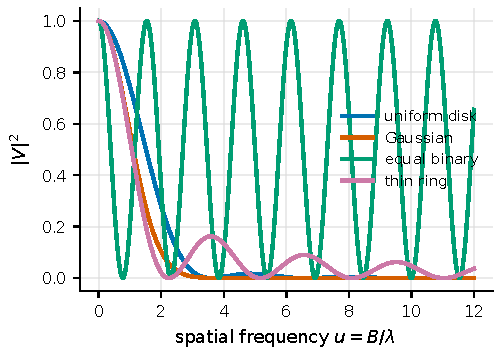
\includegraphics[width=0.88\linewidth]{figures/generated/chapter_05/ch05_vcz_visibility_models.pdf}
\caption{不同天空亮度模型在 \(|V|^2\) 空间留下不同结构。均匀圆盘有 Bessel 型零点，Gaussian 源平滑下降，等亮双星产生余弦振荡，薄环产生更密的振荡。强度干涉直接给出这些曲线的模平方，而不是复可见度本身。}
\label{fig:ch05-vcz-models}
\end{figure}

\section{从可见度曲线读出恒星角直径}

把 VCZ 定理用于恒星，最简单的模型是均匀圆盘。假设恒星角直径为 \(\theta\)，表面亮度在圆盘内为常数，在圆盘外为零。圆对称的 Fourier 变换给出
\begin{equation}
  V(B)=\frac{2J_1(x)}{x},
  \qquad
  x=\frac{\pi\theta B}{\lambda},
  \label{eq:ch05-uniform-disk}
\end{equation}
\begin{formulaexplain}
\(V(B)\) 是均匀圆盘的可见度；\(J_1\) 是一阶 Bessel 函数；\(\theta\) 是角直径，\(B\) 是投影基线。无量纲量 \(x\) 决定圆盘在该基线上被分辨到什么程度。
\end{formulaexplain}
其中 \(J_1\) 是一阶 Bessel 函数，\(\theta\) 用弧度，\(B\) 是投影基线长度，\(\lambda\) 是观测波长。式子里的无量纲组合 \(x=\pi\theta B/\lambda\) 是最重要的量：同一颗星在更长基线或更短波长下更容易被分辨，同一条基线对更大的角直径也更敏感。

均匀圆盘的第一个零点满足 \(x=3.8317\)，因此
\begin{equation}
  B_0\simeq \frac{1.22\,\lambda}{\theta}.
  \label{eq:ch05-first-null}
\end{equation}
\begin{formulaexplain}
\(B_0\) 是均匀圆盘可见度的第一零点基线；\(\lambda\) 是波长，\(\theta\) 是角直径。它给出“刚好分辨到第一个暗纹”所需的基线尺度。
\end{formulaexplain}
\(B_0\) 的单位是米。取 VERITAS 和 MAGIC 常用的蓝光波段 \(\lambda=416\,{\rm nm}\)，若 \(\theta=1\,{\rm mas}=4.848\times10^{-9}\,{\rm rad}\)，第一个零点约 \(105\,{\rm m}\)；若 \(\theta=0.5\,{\rm mas}\)，需要约 \(210\,{\rm m}\)；若 \(\theta=0.2\,{\rm mas}\)，需要约 \(520\,{\rm m}\)。这解释了为什么 Narrabri 的 10--188 m 基线能测亮的亚毫角秒恒星，而公里级 CTAO 阵列有机会进入几十微角秒角尺度 \citep{1967MNRAS.137..375H,1967MNRAS.137..393H,1974MNRAS.167..121H,1974iiia.book.....H,2006ApJ...649..399L,2014SPIE.9146E..0ZD}。

\begin{figure}[tbp]
\centering
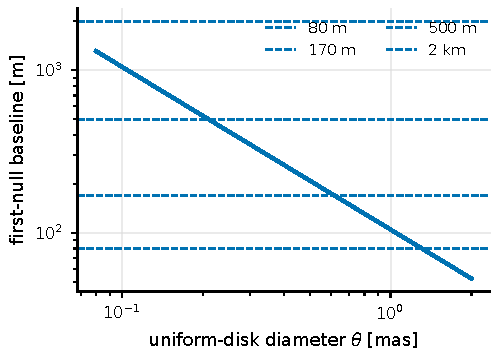
\includegraphics[width=0.86\linewidth]{figures/generated/chapter_05/ch05_uniform_disk_resolution.pdf}
\caption{均匀圆盘在 \(\lambda=416\,{\rm nm}\) 下的第一零点基线。0.5 mas 恒星需要约 210 m 才到第一个零点，0.1 mas 量级目标需要公里级基线；这正是 Cherenkov 阵列对蓝光强度干涉有吸引力的原因。}
\label{fig:ch05-uniform-disk-resolution}
\end{figure}

实际观测不会只问“零点在哪里”。最有信息的往往是第一 lobe 的下降区：短基线处 \(|V|^2\simeq1\)，不同角直径曲线几乎重合；零点以后 \(|V|^2\) 很低，系统误差和背景容易主导；下降区既有较大信号，又对 \(\theta\) 敏感。因此设计观测时通常要先画出目标模型的 \(|V(B)|^2\) 和不同角直径的差异，选择能覆盖下降区和零点附近的投影基线。

均匀圆盘也只是第一模型。热星有 limb darkening，快速自转星有赤道鼓包和 gravity darkening，Be 星有盘，双星有两个亮度中心，Cepheid 会随相位改变半径。均匀圆盘直径 \(\theta_{\rm UD}\) 常是便于比较的中间量；要得到 limb-darkened 直径 \(\theta_{\rm LD}\)，需要大气模型和波段响应。VERITAS 对 \(\beta\) CMa 和 \(\epsilon\) Ori 的首批四望远镜强度干涉结果给出 \(\theta_{\rm UD}=0.523\pm0.017\,{\rm mas}\) 和 \(0.631\pm0.017\,{\rm mas}\)，相应 limb-darkened 直径为 \(0.542\pm0.018\,{\rm mas}\) 和 \(0.660\pm0.018\,{\rm mas}\) \citep{2020NatAs...4.1164A}。后续 \(\beta\) UMa 观测和 \(\gamma\) Cas 快速自转星观测说明，随着 \(u,v\) 覆盖改善，强度干涉不只测“一个半径”，也能约束方向依赖的 photosphere 形状 \citep{2024ApJ...966...28A,2025ApJ...995..191A}。

\section{HBT 相关器真正测到什么}

前两节讨论的是一阶相干和复可见度。强度干涉真正记录的是两台望远镜的强度涨落是否同步。第 \ref{chap:04} 章的 Siegert 关系 \eqref{eq:ch04-siegert} 用到空间通道时变成
\begin{equation}
  g_{12}^{(2)}(0)-1
  =
  \zeta\,\left|\gamma_{12}^{(1)}\right|^2 .
  \label{eq:ch05-hbt-spatial}
\end{equation}
\begin{formulaexplain}
\(g_{12}^{(2)}(0)-1\) 是零延迟强度相关的超额；\(\zeta\) 是时间响应、带宽、偏振和背景等稀释因子；\(|\gamma_{12}^{(1)}|^2\) 是平方可见度。它是空间 HBT 的核心关系。
\end{formulaexplain}
\(g_{12}^{(2)}(0)-1\) 是两台望远镜零延迟强度相关的 excess；\(\gamma_{12}^{(1)}\) 是同一基线上的一阶空间相干度；\(\zeta\) 收集有限时间响应、光谱带宽、偏振、背景和仪器归一化。对热光或高斯混沌光，\(|\gamma_{12}^{(1)}|^2=|V(B)|^2\)。因此 HBT 不需要把两台望远镜的电场直接合束，却能通过强度涨落的同步程度测可见度模平方。

数据分析中常把这个关系写成观测模型
\begin{equation}
  C_{12}(B)
  \equiv g_{12}^{(2)}(0)-1
  =
  N_0\,f_1 f_2\,|V(B)|^2 ,
  \label{eq:ch05-correlation-model}
\end{equation}
\begin{formulaexplain}
\(C_{12}\) 是观测到的相关峰幅度；\(N_0\) 是零基线仪器响应；\(f_1,f_2\) 是目标光子占比；\(|V|^2\) 是天体结构项。它把仪器、背景和源结构分开。
\end{formulaexplain}
\(C_{12}(B)\) 是基线 \(B\) 上的相关峰幅度；\(N_0\) 是零基线相关幅度，也就是同一光源在没有空间分辨损失时应有的仪器响应后聚束高度；\(f_1,f_2\) 是两台望远镜中目标光子占总计数的比例；\(V(B)\) 是式 \eqref{eq:ch05-vcz} 给出的归一化可见度。这个模型把三个影响分开：天体结构给 \(|V|^2\)，背景给 \(f_1f_2\)，仪器给 \(N_0\)。

若探测器有效时间宽度为 \(\Delta t_{\rm eff}\)，光学带宽为 \(\Delta\nu\)，未分偏振热光的零基线幅度数量级为
\begin{equation}
  N_0\sim \frac{1}{2\,\Delta\nu\,\Delta t_{\rm eff}},
  \qquad
  \Delta\nu\simeq\frac{c\,\Delta\lambda}{\lambda^2}.
  \label{eq:ch05-n0}
\end{equation}
\begin{formulaexplain}
\(N_0\) 是未被空间分辨时的聚束峰高度；\(\Delta\nu\) 是光学频率带宽；\(\Delta t_{\rm eff}\) 是电子有效时间宽度。带宽和时间响应越宽，热光相关峰被平均得越低。
\end{formulaexplain}
这里的 \(1/2\) 可理解为未分辨两个偏振模式的稀释；若只选一个线偏振，偏振因子会不同。对 VERITAS 的 \(\lambda=416\,{\rm nm}\)、\(\Delta\lambda=13\,{\rm nm}\)、\(\Delta t_{\rm eff}\sim4\,{\rm ns}\)，这个估算给 \(N_0\) 为几 \(10^{-6}\)。实际拟合得到 \(N_0=(1.23\pm0.05)\times10^{-6}\) 和 \((1.26\pm0.06)\times10^{-6}\)，说明光学带宽、电子响应和系统效率共同把热光聚束峰压到百万分之一量级 \citep{2020NatAs...4.1164A}。

\begin{figure}[tbp]
\centering
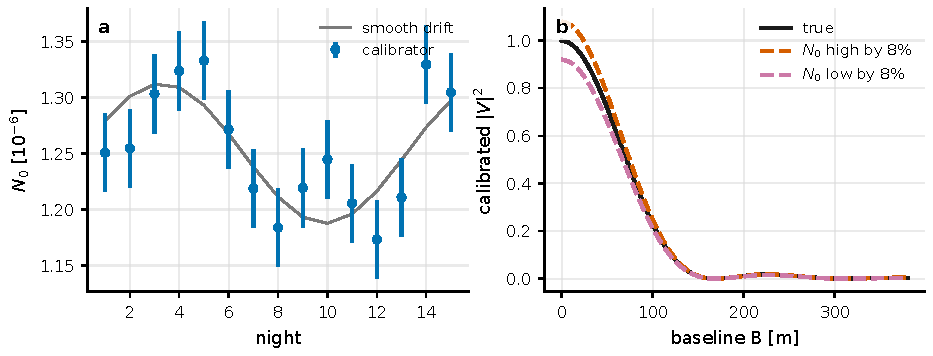
\includegraphics[width=0.92\linewidth]{figures/generated/chapter_05/ch05_zero_baseline_calibration.pdf}
\caption{零基线相关幅度 \(N_0\) 的标定对 \(|V|^2\) 的直接影响。左图示意校准星给出的夜间 \(N_0\) 漂移；右图显示 \(N_0\) 若偏高或偏低 8\%，所有基线上的 \(|V|^2\) 都会被整体拉伸，从而把角直径、边缘昏暗或扁率拟合推向错误值。}
\label{fig:ch05-zero-baseline}
\end{figure}

\begin{figure}[tbp]
\centering
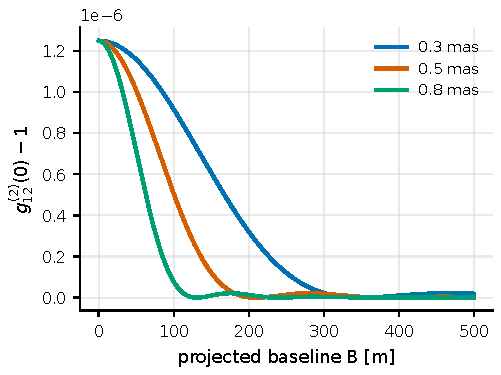
\includegraphics[width=0.86\linewidth]{figures/generated/chapter_05/ch05_sii_signal_vs_baseline.pdf}
\caption{用 \(C_{12}=N_0|V|^2\) 估算的强度干涉信号，\(N_0\) 取 \(1.25\times10^{-6}\) 的现代蓝光系统量级。角直径越大，\(|V|^2\) 越早随基线下降并出现零点；因此同一组基线对 0.8 mas 恒星比对 0.3 mas 恒星更敏感。}
\label{fig:ch05-sii-signal}
\end{figure}

强度干涉的代价是相位缺失。两台望远镜只测 \(|V|^2\)，不能像振幅干涉那样直接得到 Fourier 相位；镜像亮度分布 \(I(-l,-m)\) 与原图有相同的 \(|V|^2\)。它换来的优势是对光学路径的要求大幅降低。振幅干涉需要把光程稳定到波长的一小部分；强度干涉只需要把电子信号对齐到探测响应时间的一小部分。对 \(1\,{\rm GHz}\) 电子带宽，路径误差达到几厘米才会明显降低相关；大气 piston 在光学相位上很致命，但对 ns 量级强度相关几乎不是主噪声源。这也是为什么光学成像质量并非专用干涉仪级别的 Cherenkov 望远镜仍可用于强度干涉 \citep{2006ApJ...649..399L,2008AIPC..984..205L,2013APh....43..331D,2014SPIE.9146E..0ZD}。

\begin{figure}[tbp]
\centering
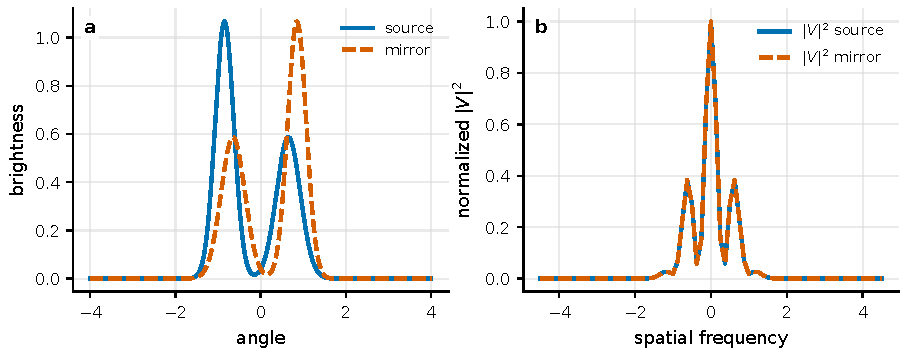
\includegraphics[width=0.92\linewidth]{figures/generated/chapter_05/ch05_phase_ambiguity.pdf}
\caption{只测 \(|V|^2\) 会丢失 Fourier 相位。左图中的源和镜像源亮度分布不同；右图中二者的 \(|V|^2\) 完全重合。强度干涉成像需要二维 \(u,v\) 覆盖、物理先验、三阶相关或相位恢复算法来打破这类退化。}
\label{fig:ch05-phase-ambiguity}
\end{figure}

\section{怎样判断一次观测是否可行}

强度干涉的统计难点来自一个事实：信号幅度很小，而随机符合数很大。Hanbury Brown 的双望远镜强度干涉信噪比常写成
\begin{equation}
  \left(\frac{S}{N}\right)_{\rm rms}
  =
  A\,\alpha\,n\,|\gamma_{12}^{(1)}|^2
  \left(\frac{\Delta f\,T}{2}\right)^{1/2}.
  \label{eq:ch05-snr}
\end{equation}
\begin{formulaexplain}
\(A\) 是收集面积，\(\alpha\) 是探测效率，\(n\) 是光子谱流量，\(\Delta f\) 是电子带宽，\(T\) 是积分时间。SNR 线性受光子数影响，却只按带宽和时间的平方根增长。
\end{formulaexplain}
\(A\) 是每台望远镜的收集面积，单位 \({\rm cm^2}\)；\(\alpha\) 是总光子探测效率，包括镜面、滤光片、量子效率和读出损失；\(n\) 是目标在观测波段的光子谱流量，单位 \({\rm photons\,s^{-1}\,cm^{-2}\,Hz^{-1}}\)；\(\Delta f\) 是电子相关带宽，单位 Hz；\(T\) 是积分时间，单位 s；\(|\gamma|^2=|V|^2\) 是基线上的平方可见度。

这个公式有两个值得记住的结论。第一，SNR 与光子谱流量、收集面积和效率成正比，所以亮星和大镜面非常重要。第二，SNR 只按 \((\Delta f T)^{1/2}\) 增长，所以把曝光从 5 小时加到 20 小时只提高 2 倍，把电子带宽从 250 MHz 提到 1 GHz 也只提高 2 倍。公式不显含光学滤光片带宽，是因为在探测器远慢于光学相干时间的极限下，窄滤光片减少光子数的同时增加相干时间，两者近似抵消；真实系统仍需把滤光片形状、背景和探测器响应放进 \(N_0\) 或完整似然中。

用式 \eqref{eq:ch05-snr} 可记住几个数量级。Le Bohec 和 Holder 估算过：两台 \(100\,{\rm m^2}\) 望远镜、\(\alpha=0.3\)、\(\Delta f=1\,{\rm GHz}\)、\(T=5\,{\rm hr}\)，在 \(|\gamma|^2=0.5\) 处可用 \(5\sigma\) 测到约 \(V=6.7\) 等星；\(V=5\) 等星的角直径精度可到几个百分点 \citep{2006ApJ...649..399L}。Narrabri 使用两台直径 \(6.5\,{\rm m}\) 的光收集器，443 nm、10 nm 滤光片和约 60 MHz 电子带宽，最终样本主要限于 \(B<2.5\) 的亮星 \citep{1967MNRAS.137..375H,1974MNRAS.167..121H,1974iiia.book.....H}。VERITAS 用四台 12 m 望远镜、250 MS/s 采样和离线相关，在明月附近的非伽马观测时间里获得了数小时级恒星直径测量 \citep{2020NatAs...4.1164A,2024ApJ...966...28A,2025ApJ...995..191A}。

\begin{figure}[tbp]
\centering
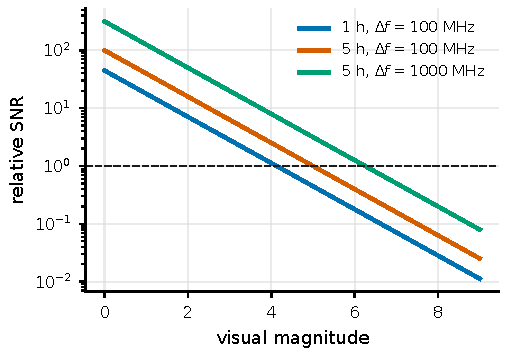
\includegraphics[width=0.86\linewidth]{figures/generated/chapter_05/ch05_snr_scaling.pdf}
\caption{强度干涉信噪比的相对标度。恒星每暗 1 等，光子谱流量约降为原来的 0.398；积分时间和电子带宽只按平方根改善 SNR。曲线未包含收集面积、效率、背景稀释和 \(|V|^2\)，显示亮星选择和高速电子学怎样限制可达信噪比。}
\label{fig:ch05-snr-scaling}
\end{figure}

背景光以两种方式伤害观测。它先增加 shot noise，又把式 \eqref{eq:ch05-correlation-model} 的振幅乘上 \(f_1f_2\)。若每台望远镜里目标光子只占总光子的 70\%，相关振幅已经降到约 0.49。要恢复同样显著性，需要更长积分，并且系统误差更容易占主导。月光、夜天光、PSF 过宽、相邻星污染和探测器暗电流都以这种方式进入。Le Bohec 和 Holder 估算过，Cherenkov 望远镜 \(0.05^\circ\) 量级的光学 PSF 会让夜天光成为暗星灵敏度边界；现代 VERITAS 分析也要修正 night-sky background 和暗电流，否则角直径可产生约 10\% 量级偏差 \citep{2006ApJ...649..399L,2020NatAs...4.1164A,2025ApJ...995..191A}。

系统相关比白噪声更危险，因为目标信号本来只有 \(10^{-6}\) 到 \(10^{-3}\)。常见检查包括：远离零延迟的相关是否为零；互换通道或人为时间偏移后峰是否消失；不同望远镜对、不同夜晚、不同月距和不同电子链路是否给出一致的 \(N_0\)；同一目标的 \(|V|^2\) 是否随投影基线而不是随 PMT 电流、温度或电子增益变化。MAGIC-SII 采用常规相机像素、窄带滤光片、VCSEL 模拟光纤传输、约 110 MHz 聚合带宽和 GPU 实时无死时间相关器，报告了 22 个恒星直径测量；这类系统把限制推向工程稳定性和校准体系，望远镜面积只是其中一项 \citep{2024MNRAS.529.4387A,2022SPIE12183E..0DK,2019ICRC...36..740M,2019ICRC...36..714K}。

\begin{figure}[tbp]
\centering
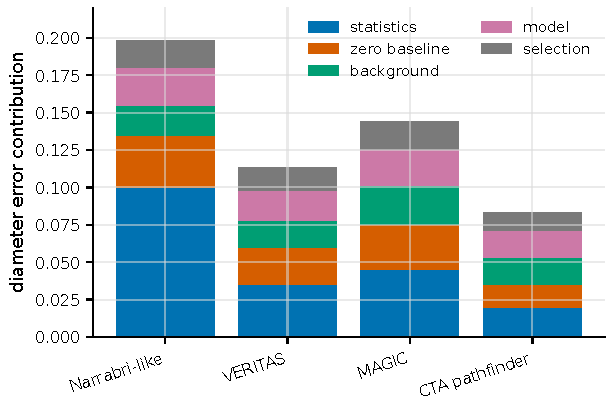
\includegraphics[width=0.82\linewidth]{figures/generated/chapter_05/ch05_error_budget.pdf}
\caption{强度干涉角直径误差预算的组成。统计误差会随光子数和积分时间下降，但零基线定标、背景稀释、恒星模型和天气/选择函数会形成系统误差地板；现代阵列的科学产出取决于这些项能否和 photon noise 一起写进似然。}
\label{fig:ch05-error-budget}
\end{figure}

\section{多基线怎样走向成像}

两台望远镜只能给一个投影基线上的 \(|V|^2\)。若阵列有 \(N\) 台望远镜，同时可形成
\begin{equation}
  N_{\rm base}=\frac{N(N-1)}{2}
  \label{eq:ch05-baseline-number}
\end{equation}
\begin{formulaexplain}
\(N_{\rm base}\) 是可同时形成的望远镜对数；\(N\) 是望远镜数量。每一对望远镜给一条基线，所以基线数随阵列规模近似按 \(N^2/2\) 增长。
\end{formulaexplain}
条基线。强度干涉在这里有一个实际优势：电信号可以复制到许多相关器，形成所有望远镜对，不像振幅干涉那样把同一束相干光分给多个合束器会损失光子。地球自转又会改变每条物理基线的天空投影，使同一望远镜对在一夜中扫过一段 \(u,v\) 轨迹。若每隔几分钟保存一次相关结果，就能把恒星的空间频率采样从几个点扩展成轨迹；多夜、多 hour angle 和多望远镜对一起构成二维 \(u,v\) 覆盖 \citep{2008AIPC..984..205L,2012MNRAS.419..172N,2012MNRAS.424.1006N,2013APh....43..331D}。

\begin{figure}[tbp]
\centering
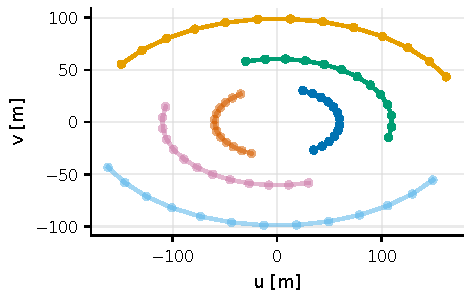
\includegraphics[width=0.82\linewidth]{figures/generated/chapter_05/ch05_uv_coverage.pdf}
\caption{固定望远镜基线在地球自转中投影到不同 \(u,v\) 位置。每条彩色轨迹代表一个望远镜对，负的共轭点也可用于实亮度分布的 Fourier 约束。覆盖越稠密，越能区分圆盘、椭圆、双星和表面斑点。}
\label{fig:ch05-uv-coverage}
\end{figure}

只测 \(|V|^2\) 并不等于只能测直径。对均匀圆盘、椭圆圆盘、双星和 limb darkening 这类低维模型，\(|V|^2\) 已经能给很强约束。若要做模型无关图像重建，则需要补充相位信息或施加图像约束。第 \ref{chap:04} 章的三阶公式 \eqref{eq:ch04-g3-closure} 对应到三台望远镜 \(1,2,3\) 时，项
\[
  2\,{\rm Re}(\gamma_{12}\gamma_{23}\gamma_{31})
\]
含有闭合三角形的相位和。这个量不受单台望远镜相位 piston 的影响，因此在概念上接近振幅干涉的 closure phase。问题是三阶信号比二阶信号弱，光子三元组比光子对少得多，误差传播也更苛刻；它更适合大型阵列和极亮目标，而不是所有观测的默认产品。另一条路线是从二维 \(|V|\) 分布用 Cauchy--Riemann、Gerchberg--Saxton 或 MIRA 等相位恢复与后处理算法重建相位。Nuñez 等人的模拟显示，明亮热星、快速自转星、双星和带表面斑点的恒星在 CTA 类 \(u,v\) 覆盖下可以恢复到有物理意义的形状参数，但结果依赖 SNR、短基线覆盖、先验掩膜和图像正则化 \citep{1966JOSA...56..441G,2012MNRAS.419..172N,2012MNRAS.424.1006N,2014SPIE.9146E..0ZD,2024NJPh...26f3014B}。

从仪器史看，Narrabri Stellar Intensity Interferometer 是第一个完整展示这套方法科学能力的系统。它用两台 \(6.5\,{\rm m}\) 光收集器在 10--188 m 可变基线上工作，滤光片中心约 443 nm、带宽 10 nm，PMT 量子效率约 25\%，有效电子带宽约 60 MHz；1960s--1970s 期间测量了 32 颗恒星的角直径和若干双星系统，最小直径约 \(0.4\,{\rm mas}\) \citep{1967MNRAS.137..375H,1967MNRAS.137..393H,1970MNRAS.148..103H,1971MNRAS.151..161H,1974MNRAS.167..121H,1974MNRAS.167..475H,1974iiia.book.....H}。它后来停用，主要受限于当时的大面积可移动光收集器、低噪声高速电子学和多基线成像能力。

现代 Cherenkov 阵列改变了硬件边界。它们本来为纳秒 Cherenkov 闪光设计，拥有 10 m 级口径、大面积镜面、快速 PMT、长基线和可接受的光学像质。VERITAS 四台 12 m 望远镜已经示范了六条同时基线的强度干涉，\(\beta\) CMa 和 \(\epsilon\) Ori 的直径精度优于 5\%，观测时间只有数小时，并且可在接近满月的非伽马观测时间运行 \citep{2020NatAs...4.1164A}。MAGIC 采用两台 17 m 抛物面望远镜和原有相机像素，系统升级后能在常规伽马观测与 SII 模式之间快速切换，并用 GPU 相关器报告了 22 个恒星直径 \citep{2024MNRAS.529.4387A}。VERITAS 对 \(\beta\) UMa 和 \(\gamma\) Cas 的后续结果把强度干涉从可行性演示推进到具体恒星物理：\(\gamma\) Cas 数据用六条基线和超过 160 pair-hours 观测测得可见 photosphere 的扁率，给出小轴直径约 \(0.43\,{\rm mas}\)、长短轴比约 1.28 和自转轴位置角约 \(116^\circ\) \citep{2024ApJ...966...28A,2025ApJ...995..191A}。

CTAO 的吸引力来自基线和基线数量。公里级基线在 350--450 nm 对应几十微角秒分辨率，几十到上百台望远镜又能带来上千条基线和密集 \(u,v\) 覆盖。它不会替代 CHARA、VLTI 等振幅干涉仪，因为灵敏度、相位和红外能力不同；它更像一个蓝光、超长基线、亮热星和快速变化天体的互补工具。它的科学产出取决于探测器带宽、时间同步、相关器吞吐、背景控制、可复现的零基线校准和面向光学干涉数据标准的数据产品 \citep{2009A&A...507.1719F,2010SPIE.7734E..1CN,2010SPIE.7734E..1TJ,2013APh....43..331D,2014SPIE.9146E..0ZD,2022icrc.confE.803K,2024SPIE13095E..0IT}。


\chapter{探测器、时钟和事件表}
\label{chap:06}

\begin{chapteropening}
第五章把强度干涉写成一个很小的相关峰，典型幅度可以只有 \(10^{-6}\)。这样的信号不会自动出现在论文图上。它先要经过镜面、滤光片、探测器、放大器、数字化器、时钟、数据格式和质量筛选。每一步都会改变事件率、时间戳、响应宽度或背景比例，因此也会改变最终的 \(g^{(2)}\)、\(|V|^2\) 或脉冲到达时刻。

本章的问题是：一台真实望远镜怎样把光子变成可复现的事件表？事件表不是普通光变曲线。它保留每个候选光子的时间、通道、波长、偏振和质量信息，使同一份数据以后还能重新分箱、重新选频、重新做延迟校正，或投影成光变曲线、功率谱、相关函数和脉冲相位。AquEYE/Iqueye、VERITAS-SII、MAGIC-SII、MKID 仪器和现代 TCSPC/White Rabbit 系统都说明了同一件事：相关函数里的时间尺度、效率因子和噪声项，最终来自探测器、电子学和时钟系统 \citep{2009JMOp...56..261B,2009A&A...508..531N,2015SPIE.9504E..0CZ,2020NatAs...4.1164A,2024MNRAS.529.4387A,2013PASP..125.1348M,2018PASP..130f5001M,2020RScI...91a3108W}。
\end{chapteropening}

\section{事件表为什么要保留原始信息}

第 \ref{chap:01} 章式 \eqref{eq:event-row} 给出了全书使用的最小事件行；第 \ref{chap:02} 章说明，把事件过早平均成图像、光谱或光变曲线，会丢掉许多联合概率。在仪器层，图像和事件表的区别很具体。图像把一段曝光内的光子数累加到像素上；事件表则保留每个触发事件的时间、探测器通道、望远镜编号、波长或滤光片、偏振通道、权重和质量标记。对普通测光，二者常常足够接近；对纳秒到皮秒计时、二阶相关、脉冲星折叠或快速遮掩，早期累加会直接删除待测信号。

Iqueye 的设计就是一个好例子。它把所有光子以时间标签保存下来，然后离线选择从 24.41 ps 到分钟级的任意时间 bin。对 \(\zeta\) Ori 的观测产生约 \(2\times10^{10}\) 个光子事件，数据量约 78 GB \citep{2009A&A...508..531N,2019CoSka..49...85Z}。这说明事件表不是小型辅助文件，而是真实望远镜会面对的主要数据产品。

原始事件可以写成
\begin{equation}
  \mathcal{E}^{\rm raw}_q =
  \left(n_q,\ a_q,\ d_q,\ c_q,\ p_q,\ f_q,\ w_q\right),
  \qquad
  t^{\rm raw}_q=t_0+n_q\,\delta t+\epsilon_{\rm roll}.
  \label{eq:ch06-raw-event}
\end{equation}
\begin{formulaexplain}
\(\mathcal E_q^{\rm raw}\) 是第 \(q\) 个原始事件；\(n_q\) 是时钟 tick，\(\delta t\) 是 tick 时长，\(t_0\) 是段起点，\(\epsilon_{\rm roll}\) 处理计数器溢出。它把电子记录变成最早的事件时间。
\end{formulaexplain}
下标 \(q\) 标记第 \(q\) 个事件。\(n_q\) 是电子计数器的整数时钟 tick；\(\delta t\) 是一个 tick 对应的时间，单位是秒；\(t_0\) 是记录段的起始时间；\(\epsilon_{\rm roll}\) 处理计数器溢出、分段或 rollover。现代时间数字转换器可在 \(10^{-11}\)--\(10^{-10}\,{\rm s}\) 量级取样，商用多通道 TCSPC 系统的基本时间分辨率可为 80 ps，Iqueye 的 TDC 量化步长为 24.41 ps \citep{2009A&A...508..531N,2020RScI...91a3108W}。\(a_q\) 是望远镜或站点编号，\(d_q\) 是探测器编号，\(c_q\) 是波长通道或滤光片编号，\(p_q\) 是偏振通道，\(f_q\) 是质量标记，\(w_q\) 是事件权重。溢出、丢包、饱和、云、指向异常和电子学异常都应进入 \(f_q\)，否则后续相关函数中的异常峰很难被追溯。

\begin{figure}[tbp]
\centering
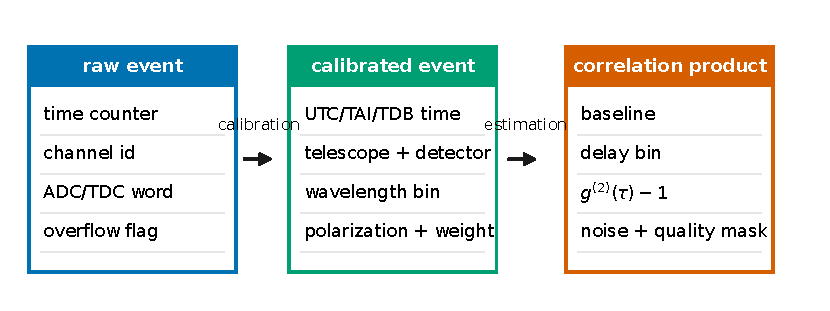
\includegraphics[width=0.96\linewidth]{figures/generated/chapter_06/ch06_event_table_schema.pdf}
\caption{事件数据从原始电子记录流向标定事件表，再流向相关函数产品。原始层保存计数器时间、通道编号和溢出标记；标定层把时间转换到统一时间尺度，并加入望远镜、波长、偏振和权重；相关产品层才记录基线、延迟 bin、相关幅度和噪声估计。若在第一层就只保存光变曲线，后面的时钟、波长和偏振选择都无法重新执行。}
\label{fig:ch06-event-table-schema}
\end{figure}

标定事件表把原始计数器时间变成可比较的物理时间：
\begin{equation}
  t^{\rm cal}_q =
  t^{\rm raw}_q
  +\Delta_{\rm clk}(t_q)
  +\Delta_{\rm elec}(a_q,d_q)
  +\Delta_{\rm det}(\lambda_q,d_q)
  -\frac{\mathbf{r}_{a_q}(t_q)\cdot\hat{\mathbf{s}}}{c}.
  \label{eq:ch06-calibrated-time}
\end{equation}
\begin{formulaexplain}
\(t_q^{\rm cal}\) 是校正后的事件时间；\(\Delta_{\rm clk}\)、\(\Delta_{\rm elec}\)、\(\Delta_{\rm det}\) 分别改正时钟、电子链路和探测器延迟；最后一项扣除几何光行时。它把不同站点放到共同时间轴。
\end{formulaexplain}
\(\Delta_{\rm clk}\) 是站点时钟相对统一时间尺度的偏移，单位秒；短时间内可以是几十皮秒到纳秒，跨夜合并时还要处理 GPS、TAI、UTC、TT 或 TDB 的转换。\(\Delta_{\rm elec}\) 是电缆、放大器、鉴别器、ADC/TDC 通道产生的固定或缓慢漂移延迟，常用脉冲源和环回链路标定。\(\Delta_{\rm det}\) 是探测器内部延迟，可能依赖波长、偏置电压、温度和脉冲高度；SNSPD 的探测延迟甚至会随光子能量变化 \citep{2020NaPho..14..250K,2020Optic...7.1649R}。最后一项是几何延迟，\(\mathbf{r}_{a_q}\) 是站点相对参考点的位置向量，\(\hat{\mathbf{s}}\) 是源方向单位向量，\(c\) 是光速。100 m 基线给出最高约 333 ns 的几何延迟，1 km 基线给出约 \(3.3\,\mu{\rm s}\)，远大于皮秒级探测器抖动。

数据率由事件率和每个事件占用的字节数决定：
\begin{equation}
  \dot{M}
  \simeq
  N_{\rm tel}\,N_{\rm ch}\,R_{\rm evt}\,N_{\rm byte}.
  \label{eq:ch06-data-rate}
\end{equation}
\begin{formulaexplain}
\(\dot M\) 是数据率；\(N_{\rm tel}\) 是望远镜数，\(N_{\rm ch}\) 是通道数，\(R_{\rm evt}\) 是单通道事件率，\(N_{\rm byte}\) 是每事件字节数。它估算事件表或波形流的存储压力。
\end{formulaexplain}
\(\dot M\) 的单位是 byte s\(^{-1}\)。\(N_{\rm tel}\) 是望远镜数，\(N_{\rm ch}\) 是每台望远镜的独立通道数，\(R_{\rm evt}\) 是单通道事件率，\(N_{\rm byte}\) 是每个事件的存储大小。如果 \(N_{\rm tel}=4\)、\(N_{\rm ch}=8\)、\(R_{\rm evt}=10^6\,{\rm s^{-1}}\)、\(N_{\rm byte}=16\) byte，则 \(\dot M\simeq512\,{\rm MB\,s^{-1}}\)。连续波形采样会更高：VERITAS-SII 以 250 MS/s 连续数字化每台望远镜的 PMT 信号，单望远镜数据流约 250 MB/s，整次实验的数据量达到几十 TB \citep{2020NatAs...4.1164A}。事件表、波形流和实时相关器可以共存，区别在于压缩、筛选和相关计算发生在数据链的哪个阶段。

\Needspace{16\baselineskip}
\section{探测器怎样塑造事件率和间隔}

探测器的第一项作用是决定有多少入射光子变成电子事件。一个通道的平均探测率可写成
\begin{equation}
  R_{\rm det}
  =
  A_{\rm eff}
  \int_{\lambda_1}^{\lambda_2}
  F_\lambda(\lambda)\,
  T_{\rm opt}(\lambda)\,
  \eta_{\rm det}(\lambda)\,
  d\lambda
  +R_{\rm sky}+R_{\rm dark}.
  \label{eq:ch06-detected-rate}
\end{equation}
\begin{formulaexplain}
\(R_{\rm det}\) 是探测计数率；\(A_{\rm eff}\) 是有效面积；\(F_\lambda\)、\(T_{\rm opt}\)、\(\eta_{\rm det}\) 描述源光子、光路透过率和探测效率；\(R_{\rm sky},R_{\rm dark}\) 是背景。它给出事件率预算。
\end{formulaexplain}
\(A_{\rm eff}\) 是有效集光面积，单位 m\(^2\)；\(F_\lambda\) 是源的光子谱通量密度，单位 photons s\(^{-1}\) m\(^{-2}\) nm\(^{-1}\)；\(T_{\rm opt}\) 是镜面、滤光片、光纤、准直器和窗口的总透过率；\(\eta_{\rm det}\) 是探测器量子效率；\(R_{\rm sky}\) 是天空背景和杂散光计数率；\(R_{\rm dark}\) 是暗计数率。强度干涉的信噪比由源光子率和背景稀释后的强度起伏共同决定。MAGIC-SII 直接用 PMT 直流电流估计光子通量，并用背景像素修正夜天光贡献；VERITAS-SII 用 off-source 测量估计背景，再把相关幅度按恒星光占比修正 \citep{2020NatAs...4.1164A,2024MNRAS.529.4387A}。

不同探测器适合不同任务。PMT 的优势是面积大、增益高、ns 级脉冲和 Cherenkov 望远镜高速电子链路兼容；蓝光量子效率常在 \(20\%\)--\(40\%\)，VERITAS-SII 在 416 nm 使用的 PMT 量子效率约 \(30\%\) \citep{2020NatAs...4.1164A,2024MNRAS.529.4387A}。SPAD 把单光子吸收后的雪崩脉冲作为事件，可见光量子效率可达 \(50\%\)--\(60\%\)，单光子时间分辨率约 30--50 ps，暗计数常见范围为 10--100 s\(^{-1}\)，但有效面积小、死时间较长，afterpulsing 会污染短延迟相关 \citep{1996ApOpt..35.1956C,2009JMOp...56..261B,2009A&A...508..531N,2015SPIE.9504E..0CZ}。SNSPD 在低暗计数和皮秒计时上最强，文献中已展示 400 nm 处 \(2.7\pm0.2\) ps 和 1550 nm 处 \(4.6\pm0.2\) ps 的系统抖动，也有 1550 nm 附近系统探测效率超过 \(90\%\) 的器件，但低温、光纤耦合和阵列读出仍是工程代价 \citep{2012SuScT..25f3001N,2020NaPho..14..250K,2020Optic...7.1649R}。MKID 牺牲时间分辨率，换取每个光子的能量信息，ARCONS 的 photon list 包含时间戳、天空坐标、波长和质量标记，典型光谱分辨率 \(R\sim8\)--10，时间精度约 \(2\,\mu{\rm s}\) \citep{2013PASP..125.1348M,2018PASP..130f5001M}。

\begin{figure}[tbp]
\centering
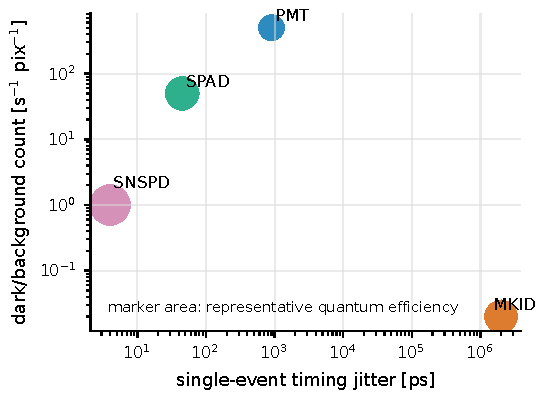
\includegraphics[width=0.70\linewidth]{figures/generated/chapter_06/ch06_detector_trade_space.pdf}
\caption{四类单光子探测技术的典型工作区域。横轴是单事件时间抖动，纵轴是每像素暗计数或背景计数的代表值，点面积表示代表性量子效率。PMT 适合大口径、高通量和 ns 级强度干涉；SPAD 给出几十皮秒计时但受面积和死时间限制；SNSPD 在低暗计数和皮秒计时上最强，但需要低温系统；MKID 牺牲时间分辨率，换取每个光子的能量信息和阵列化。}
\label{fig:ch06-detector-trade-space}
\end{figure}

效率决定事件数，死时间决定事件间隔统计是否还忠实于入射光场。非延长死时间模型给出
\begin{equation}
  R_{\rm obs}=\frac{R_{\rm in}}{1+R_{\rm in}\tau_d},
  \label{eq:ch06-nonparalyzable}
\end{equation}
\begin{formulaexplain}
\(R_{\rm in}\) 是入射事件率，\(R_{\rm obs}\) 是记录事件率，\(\tau_d\) 是死时间。非延长模型中，死时间内来的事件被丢弃，但不会延长探测器恢复时间。
\end{formulaexplain}
延长死时间模型给出
\begin{equation}
  R_{\rm obs}=R_{\rm in}\exp(-R_{\rm in}\tau_d).
  \label{eq:ch06-paralyzable}
\end{equation}
\begin{formulaexplain}
这也是死时间模型，但每个死时间内到来的新事件会重新触发恢复窗口。高通量时 \(R_{\rm obs}\) 可能先饱和再下降，因此必须知道真实探测器属于哪类响应。
\end{formulaexplain}
\(R_{\rm in}\) 和 \(R_{\rm obs}\) 的单位都是 s\(^{-1}\)，\(\tau_d\) 是死时间，单位秒。若 \(\tau_d=20\,{\rm ns}\)，非延长模型在 \(R_{\rm in}=10^7\,{\rm s^{-1}}\) 时已经让观测率比入射率低约 \(17\%\)；若 \(R_{\rm in}=10^8\,{\rm s^{-1}}\)，观测率接近饱和。SPAD 常见死时间为几十 ns 到几百 ns，MKID 可到 \(100\,\mu{\rm s}\) 量级，现代 TCSPC 电子学本身可以把通道死时间压到 650 ps，但探测器脉冲宽度和前端电子仍会限制真实高通量能力 \citep{2009A&A...508..531N,2013PASP..125.1348M,2020RScI...91a3108W}。

\begin{figure}[tbp]
\centering
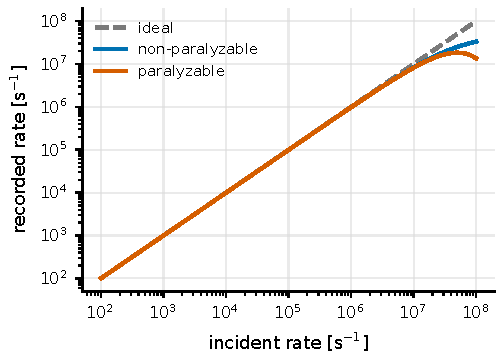
\includegraphics[width=0.70\linewidth]{figures/generated/chapter_06/ch06_deadtime_saturation.pdf}
\caption{入射计数率升高时，死时间使记录计数率偏离理想直线。非延长模型趋向饱和，延长模型在极高通量下反而下降。图中采用 \(\tau_d=20\,{\rm ns}\)，代表高速单光子通道的数量级；真实仪器需要用脉冲源或稳定光源单独测量 \(\tau_d\) 和模型类型。}
\label{fig:ch06-deadtime-saturation}
\end{figure}

afterpulsing 是另一种短延迟污染。雪崩器件中滞留载流子会在主脉冲后释放，产生与真实天体光子无关的二次事件。若每个真实事件产生 afterpulse 的概率为 \(\epsilon_{\rm ap}\)，延迟分布为归一化核 \(k_{\rm ap}(\tau)\)，额外事件率可写成
\begin{equation}
  R_{\rm ap}(\tau)=\epsilon_{\rm ap}\,R_{\rm det}\,k_{\rm ap}(\tau),
  \qquad
  \int_0^\infty k_{\rm ap}(\tau)\,d\tau=1.
  \label{eq:ch06-afterpulse}
\end{equation}
\begin{formulaexplain}
\(R_{\rm ap}\) 是 afterpulse 贡献；\(\epsilon_{\rm ap}\) 是每个真实事件产生伪脉冲的概率；\(k_{\rm ap}\) 是归一化延迟核。它描述探测器自身制造的短延迟假相关。
\end{formulaexplain}
\(\epsilon_{\rm ap}\) 无量纲，常在 \(10^{-4}\)--\(10^{-2}\) 范围内随器件和门控方式变化；\(k_{\rm ap}\) 的特征时间可从 ns 到 \(\mu{\rm s}\)。同一探测器的自相关会直接看到 afterpulse 峰，两个独立探测器的互相关则大幅降低这类污染。HBT 分束和多通道交叉相关因此有两层作用：提高可承受计数率，同时压制同通道死时间和 afterpulsing \citep{1957RSPSA.242..300B,1996ApOpt..35.1956C,2020RScI...91a3108W}。

\Needspace{14\baselineskip}
时间响应把真实相关峰卷积成更宽的峰。若两个通道的时间响应分别为 \(h_1(t)\) 和 \(h_2(t)\)，观测到的二阶相关超额近似为
\begin{equation}
  C^{\rm obs}_{12}(\tau)
  =
  \int C^{\rm sky}_{12}(\tau')\,
  h_{12}(\tau-\tau')\,d\tau',
  \qquad
  h_{12}=h_1*h_2.
  \label{eq:ch06-response-convolution}
\end{equation}
\begin{formulaexplain}
\(C^{\rm sky}_{12}\) 是天体真实相关，\(C^{\rm obs}_{12}\) 是观测结果；\(h_1,h_2\) 是两通道时间响应，\(h_{12}\) 是合成响应。仪器会把窄相关峰卷积展宽。
\end{formulaexplain}
\(C_{12}=g^{(2)}_{12}-1\) 无量纲，\(\tau\) 和 \(\tau'\) 的单位是秒。若响应函数近似高斯，宽度预算可写成
\begin{equation}
  \sigma_{\rm obs}^2
  \simeq
  \sigma_{\rm sky}^2+\sigma_1^2+\sigma_2^2+\sigma_{\rm opt}^2+\sigma_{\rm clk}^2 .
  \label{eq:ch06-jitter-budget}
\end{equation}
\begin{formulaexplain}
\(\sigma_{\rm obs}\) 是观测峰宽；\(\sigma_{\rm sky}\) 是源自身宽度；\(\sigma_1,\sigma_2\)、\(\sigma_{\rm opt}\)、\(\sigma_{\rm clk}\) 分别来自探测器、光路和时钟。独立高斯展宽按方差相加。
\end{formulaexplain}
\(\sigma_{\rm sky}\) 是光源自身相干时间或脉冲宽度，\(\sigma_1,\sigma_2\) 是探测器和电子通道的 rms 抖动，\(\sigma_{\rm opt}\) 是镜面等时性和光路展宽，\(\sigma_{\rm clk}\) 是两站时钟残差。VERITAS 的 Davies-Cotton 镜面和 PMT 脉冲宽度使强度相关峰可用 \(\sigma_\tau\simeq4\,{\rm ns}\) 的高斯描述；MAGIC-SII 相关峰的高斯宽度约 \(2.2\,{\rm ns}\)，并用自相关长期跟踪电子带宽稳定性 \citep{2020NatAs...4.1164A,2024MNRAS.529.4387A}。

\begin{figure}[tbp]
\centering
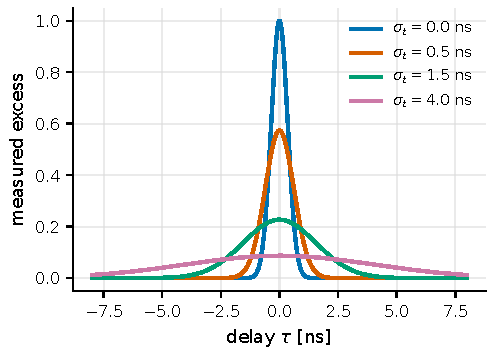
\includegraphics[width=0.70\linewidth]{figures/generated/chapter_06/ch06_detector_timing_response.pdf}
\caption{有限时间响应会把窄相关峰展宽并降低峰高。曲线保持峰面积近似不变，只改变 rms 抖动 \(\sigma_t\)。当真实相干时间远短于 ns 级电子响应时，峰宽主要由仪器决定，峰高按展宽因子被稀释；这正是强度干涉中需要高电子带宽和稳定响应函数的原因。}
\label{fig:ch06-detector-timing-response}
\end{figure}

\section{时钟和几何延迟怎样建立共同时间轴}

两台望远镜的事件表只有放到共同时间轴上才可以相关。短基线强度干涉主要要求相对延迟稳定，脉冲星计时、快速暂现源和跨夜合并还要求绝对时间可追溯到标准时间尺度。AquEYE/Iqueye 采用铷钟和 GPS PPS，把相对时间精度做到约 100 ps rms，把绝对 UTC 精度控制在 \(0.5\,{\rm ns}\) 以内；现代多通道时间标记器可接入 White Rabbit 光纤网络，5 km 光纤链路测试得到约 39 ps 的同步贡献 \citep{2009A&A...508..531N,2015SPIE.9504E..0CZ,2013NIMPA.725..187J,2020RScI...91a3108W}。

\Needspace{13\baselineskip}
对一对站点 \(a,b\)，几何延迟为
\begin{equation}
  \Delta t_{\rm geo}(t)
  =
  \frac{\mathbf{B}_{ab}(t)\cdot\hat{\mathbf{s}}}{c},
  \qquad
  \mathbf{B}_{ab}=\mathbf{r}_b-\mathbf{r}_a .
  \label{eq:ch06-geometric-delay}
\end{equation}
\begin{formulaexplain}
\(\Delta t_{\rm geo}\) 是两站几何延迟；\(\mathbf B_{ab}\) 是基线向量，\(\hat{\mathbf s}\) 是源方向，\(c\) 是光速。它把空间基线投影成两路事件表需要相互平移的时间量。
\end{formulaexplain}
\(\mathbf{B}_{ab}\) 的单位是 m，\(\hat{\mathbf{s}}\) 无量纲，\(\Delta t_{\rm geo}\) 的单位是秒。地球自转会让投影基线随时间变化，所以几何延迟也随时间漂移。一个 100 m 基线在天顶附近的延迟变化速度约为 \(\Omega_\oplus B/c\sim2.4\times10^{-11}\,{\rm s\,s^{-1}}\)，17 分钟内可漂移几十 ps；对 km 基线或皮秒级相关峰，这个变化不能只用一个常数延迟吸收。VERITAS-SII 对每个相关帧移动时间 lag 来校正几何光程，MAGIC-SII 在 Pearson 相关后应用可变时间延迟校正 \citep{2020NatAs...4.1164A,2024MNRAS.529.4387A}。

若要把事件折叠到脉冲星相位，或把光子到达时刻与其他波段比较，站点时间还要转换到太阳系质心。概念上可写为
\begin{equation}
  t_{\rm SSB}
  =
  t_{\rm site}
  +\Delta_{\rm C}
  +\Delta_{\rm R}
  +\Delta_{\rm E}
  +\Delta_{\rm S}
  +\Delta_{\rm A}.
  \label{eq:ch06-barycentric-time}
\end{equation}
\begin{formulaexplain}
\(t_{\rm SSB}\) 是太阳系质心到达时；\(t_{\rm site}\) 是站点时间；各 \(\Delta\) 项修正时钟、Roemer、Einstein、Shapiro 和大气延迟。它用于跨夜、跨波段和脉冲相位比较。
\end{formulaexplain}
\(\Delta_{\rm C}\) 是本地时钟到标准原子时和坐标时的校正，包含 UTC 到 TAI、TT、TDB 或 TCB 的时间尺度转换和闰秒；\(\Delta_{\rm R}\) 是 Roemer 光行时，地球绕太阳运动给出最高约 \(\pm500\,{\rm s}\) 的投影项；\(\Delta_{\rm E}\) 是 Einstein 延迟，来自引力势和运动导致的钟速变化；\(\Delta_{\rm S}\) 是太阳系天体的 Shapiro 延迟；\(\Delta_{\rm A}\) 是大气传播延迟。Tempo2 把这些项实现到 ns 级，barycorrpy 和 Astropy 则给出 Python 工作流中的时间尺度和质心速度/时间改正接口 \citep{2006MNRAS.369..655H,2006MNRAS.372.1549E,2018RNAAS...2....4K,2013A&A...558A..33A,2018AJ....156..123A}。

\begin{figure}[tbp]
\centering
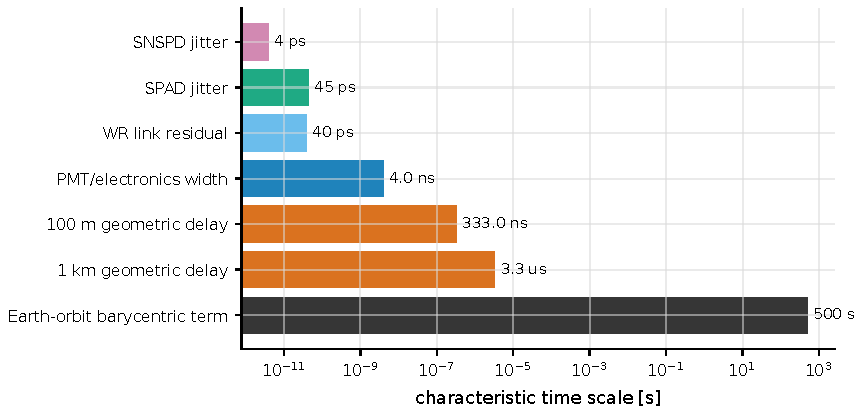
\includegraphics[width=0.82\linewidth]{figures/generated/chapter_06/ch06_time_budget.pdf}
\caption{同一份事件表会同时遇到皮秒、纳秒、微秒和百秒量级的时间项。探测器抖动和 White Rabbit 残差决定相关峰能否保持窄形；电子和镜面响应决定 ns 级强度干涉峰宽；几何延迟由基线长度和源方向决定；太阳系质心改正虽然对同夜强度相关不是峰宽项，却是脉冲星相位、跨夜合并和多信使比较的绝对时间基础。}
\label{fig:ch06-time-budget}
\end{figure}

\Needspace{16\baselineskip}
\section{光谱、偏振和背景为什么也要进事件表}

窄带滤光片、分色镜、光纤光谱仪和 MKID 都是在事件表里给每个光子增加频率信息。光谱通道的中心波长 \(\lambda\)、宽度 \(\Delta\lambda\) 和形状 \(S(\lambda)\) 决定相干时间。若通道近似矩形，数量级关系为
\begin{equation}
  \tau_c
  \simeq
  \frac{1}{\Delta\nu}
  \simeq
  \frac{\lambda^2}{c\,\Delta\lambda}
  =
  \frac{R\,\lambda}{c},
  \qquad
  R=\frac{\lambda}{\Delta\lambda}.
  \label{eq:ch06-coherence-time}
\end{equation}
\begin{formulaexplain}
\(\tau_c\) 是相干时间；\(\Delta\nu\) 是频率带宽；\(\lambda,\Delta\lambda\) 是中心波长和带宽；\(R\) 是光谱分辨率。窄通道让相位记忆变长，但单通道光子率变低。
\end{formulaexplain}
\(\tau_c\) 的单位是秒。以 \(\lambda=500\,{\rm nm}\) 为例，\(R=100\) 给出 \(\tau_c\simeq0.17\,{\rm ps}\)，\(R=10^4\) 给出 \(\tau_c\simeq17\,{\rm ps}\)，\(R=10^5\) 给出 \(\tau_c\simeq170\,{\rm ps}\)。这些数仍短于多数 PMT/电子链的 ns 响应，所以实际相关峰宽通常由仪器决定，峰高则包含电子带宽与光学带宽的比值。VERITAS 使用中心 416 nm、有效宽度 13 nm 的滤光片；MAGIC 使用 425 nm、26 nm 干涉滤光片，但快光束入射角会改变实际通带形状 \citep{2020NatAs...4.1164A,2024MNRAS.529.4387A,1974iiia.book.....H}。

\begin{figure}[tbp]
\centering
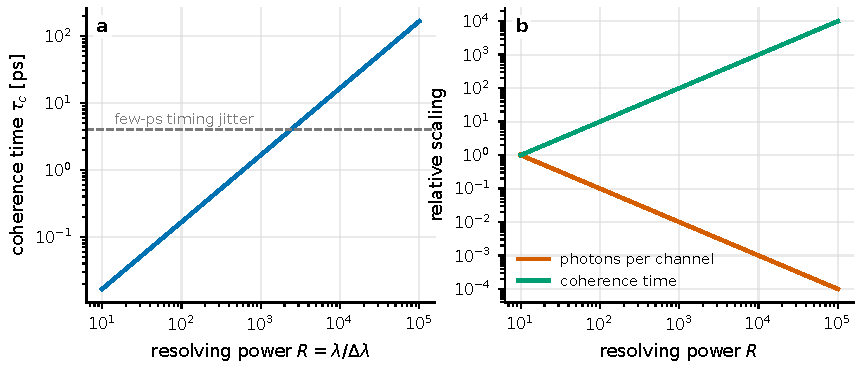
\includegraphics[width=0.92\linewidth]{figures/generated/chapter_06/ch06_spectral_resolution_coherence.pdf}
\caption{光谱分辨率和相干时间的数量级关系。左图固定 \(\lambda=500\,{\rm nm}\)，显示 \(\tau_c\simeq R\lambda/c\) 随分辨率线性增长；右图显示单个通道的光子率约随 \(1/R\) 降低，而相干时间随 \(R\) 增加。理想强度干涉信噪比对光学带宽的依赖会部分抵消，但真实仪器还受到滤光片形状、探测器响应、背景和电子带宽限制。}
\label{fig:ch06-spectral-resolution-coherence}
\end{figure}

提高 \(R\) 会拉长 \(\tau_c\)，但会减少单通道光子率；若要保留总通量，需要同时读出更多波长通道。多通道 TCSPC 可以把不同波长通道作为独立输入，并输出单一时间排序的数据流；MAGIC 和 VERITAS 的 SII 系统则选择少数宽滤光片通道换取更高光子率 \citep{2020RScI...91a3108W,2020NatAs...4.1164A,2024MNRAS.529.4387A}。对恒星直径测量，宽通道提高信噪比；对发射线、吸收线、快速旋转星或风结构，分波长相关可能直接给出空间信息随速度的变化。

偏振通道记录的是电场方向的投影。若仪器把两个正交线偏振 \(H,V\) 分开，最简单的计数估计为
\begin{equation}
  I=R_H+R_V,\qquad Q=R_H-R_V .
  \label{eq:ch06-stokes-hv}
\end{equation}
\begin{formulaexplain}
\(R_H,R_V\) 是两个正交线偏振通道的计数率；\(I\) 是总强度，\(Q\) 是水平和垂直偏振差。分偏振事件表可以在后处理中重建 Stokes 信息。
\end{formulaexplain}
若再用 \(45^\circ/135^\circ\) 和左/右圆偏振通道，可估计 \(U\) 和 \(V\)。这里的 \(R_p\) 是偏振通道 \(p\) 的背景扣除计数率，单位 s\(^{-1}\)。真实仪器还要引入 Mueller 矩阵 \(M_{ij}\)，把望远镜反射、偏振片消光比、波片相位误差和探测器效率差写成
\begin{equation}
  \mathbf{S}_{\rm obs}=M\,\mathbf{S}_{\rm sky}+\mathbf{b},
  \label{eq:ch06-mueller}
\end{equation}
\begin{formulaexplain}
\(\mathbf S_{\rm sky}\) 和 \(\mathbf S_{\rm obs}\) 是天空与观测 Stokes 向量；\(M\) 是仪器 Mueller 矩阵；\(\mathbf b\) 是背景偏置。它把偏振串扰和效率差写成可标定模型。
\end{formulaexplain}
\(\mathbf{S}=(I,Q,U,V)^T\)，\(\mathbf{b}\) 是背景和偏置。偏振强度干涉可以比较 \(HH\) 或 \(VV\) 的相关，也可以构造交叉偏振相关，用来区分天体偏振结构和仪器串扰；一旦事件表只保存总光强，这些检验就无法重新执行。

通量和背景也必须随时间进入元数据。式 \eqref{eq:ch06-detected-rate} 中的 \(R_{\rm sky}\) 会随月相、云、视场、滤光片和地平高度变化。对大气 Cherenkov 望远镜，亮月期间反而常常是 SII 的可用时间，因为 gamma-ray 模式受夜天光限制会停观；但夜天光进入 PMT 后仍会稀释恒星相关。若 \(\beta_i=R_{{\rm bkg},i}/R_{*,i}\)，两台望远镜的背景稀释因子近似为
\begin{equation}
  |g^{(1)}_*|^2
  \simeq
  |g^{(1)}_{\rm meas}|^2
  (1+\beta_1)(1+\beta_2),
  \label{eq:ch06-background-dilution}
\end{equation}
\begin{formulaexplain}
\(|g_*^{(1)}|^2\) 是扣除背景后的恒星平方相干度；\(|g_{\rm meas}^{(1)}|^2\) 是测得值；\(\beta_i\) 是第 \(i\) 台望远镜的背景/恒星计数比。背景会把真实相关稀释掉。
\end{formulaexplain}
前提是恒星-背景和背景-背景起伏在两站之间不相关。这个式子里的 \(R_*\) 和 \(R_{\rm bkg}\) 应来自同一通道、同一增益状态和相近时间的测量；否则背景修正会把慢变增益误认为天体相关幅度 \citep{2020NatAs...4.1164A,2024MNRAS.529.4387A}。

\section{标定和数据格式怎样保证可复现}

探测器响应要先在实验室和天空上固定下来。暗场给出 \(R_{\rm dark}\) 和热背景；稳定连续光源给出线性范围和死时间曲线；弱脉冲激光给出 \(h(t)\)、通道间固定延迟和时间 walk；分束到两个独立探测器的零基线实验给出电子相关峰和 afterpulsing 的区别。对强度干涉，错延迟、错偏振、off-source 背景和远离零延迟的 lag 都应作为 null test。VERITAS-SII 在每个 1 s 相关帧中剔除高频电子噪声污染，MAGIC-SII 用无光子输入和远离信号延迟的相关来估计残余电子相关，并用自相关监测电子带宽稳定性 \citep{2020NatAs...4.1164A,2024MNRAS.529.4387A}。

时间和坐标元数据决定这些标定几年后还能不能复现。一个可复现的事件表至少应保存：站点地理坐标和高度；望远镜姿态和基线；原始时钟源、频率标准、闰秒表版本和时间尺度；每个通道的电子延迟、探测器偏置、高压、温度和死时间模型；滤光片或光谱响应曲线；偏振模块角度和 Mueller 标定；质量标记定义；软件版本和选择条件。FITS 标准允许用 BINTABLE 扩展保存 time-tagged photon events，并用 header 关键字描述数据含义；Astropy 提供 FITS、坐标和时间处理接口，适合把事件表、时间尺度转换和质心改正放入同一 Python 分析链 \citep{2010A&A...524A..42P,2013A&A...558A..33A,2018AJ....156..123A}。

FITS 适合长期归档和与天文软件互操作，HDF5 或 Parquet 适合高吞吐量分析和列式筛选。无论格式如何，原始事件、标定事件和相关产品最好分层保存。原始层不可被后处理覆盖；标定层记录每个版本的校正结果；相关产品层记录 bin 宽、延迟网格、权重、剔除条件和协方差。这样，一个读者可以从同一份原始数据重新生成光变曲线、\(g^{(2)}(\tau)\)、空间可见度或脉冲到达时刻，而不需要猜测早期分析脚本做了哪些隐含选择。


\chapter{事件表的数据分析}
\label{chap:07}

\begin{chapteropening}
第 \ref{chap:06} 章说明了望远镜怎样把光子候选写成带时间、通道、波长、偏振和质量标记的事件表。现在的问题是：怎样从这张表中得到可检验的科学量？同一份事件表可以投影成光变曲线，可以构造延迟直方图，也可以拟合二阶相关峰、平方可见度或脉冲到达时刻。分析层的选择决定了哪些信息被保留，哪些信息被平均掉。

本章从一个原则出发：先明确数据向量和概率模型，再计算估计量。Iqueye/AquEYE 的光子时间标签、VERITAS-SII 的离线 FPGA 相关、MAGIC-SII 的 GPU 实时 Pearson 相关，以及 Bayesian Blocks 和 Poisson likelihood 的天文统计框架，处理的都是同一个问题：怎样把事件表里的时间和通道信息变成带误差、可复现、可拟合的科学量 \citep{2009A&A...508..531N,2009JMOp...56..261B,2020NatAs...4.1164A,2024MNRAS.529.4387A,1979ApJ...228..939C,2013ApJ...764..167S}。
\end{chapteropening}

\section{事件表先变成概率模型}

沿用第 \ref{chap:06} 章的原始和标定事件表，分析层把一份标定后的事件表简写为
\begin{equation}
  \mathcal{D}
  =
  \left\{
  t_q,\ a_q,\ d_q,\ c_q,\ p_q,\ w_q,\ f_q
  \right\}_{q=1}^{N_{\rm evt}},
  \label{eq:ch07-event-data}
\end{equation}
\begin{formulaexplain}
\(\mathcal D\) 是标定后的事件表；每个 \(q\) 事件保留时间、站点、探测器、光谱、偏振、权重和质量标记；\(N_{\rm evt}\) 是事件总数。它是后续所有估计量的原始数据向量。
\end{formulaexplain}
\(t_q\) 是统一时间尺度上的到达时刻，单位秒；\(a_q\) 是望远镜或站点编号；\(d_q\) 是探测器通道；\(c_q\) 是光谱通道；\(p_q\) 是偏振通道；\(w_q\) 是权重；\(f_q\) 是质量标记。这些字段的仪器来源、时钟校正和格式要求分别见式 \eqref{eq:ch06-raw-event}、\eqref{eq:ch06-calibrated-time} 和第 \ref{chap:06} 章末的数据格式讨论。

分析的第一步不是画图，而是定义选择函数：
\begin{equation}
  S_q =
  S(t_q,a_q,d_q,c_q,p_q,f_q),
  \qquad
  S_q \in \{0,1\}\ {\rm or}\ [0,1].
  \label{eq:ch07-selection}
\end{equation}
\begin{formulaexplain}
\(S_q\) 是第 \(q\) 个事件的选择函数；自变量是事件时间、通道和质量标记。取 0/1 时表示剔除或保留，取连续值时表示曝光、背景或效率权重。
\end{formulaexplain}
二值 \(S_q\) 表示保留或剔除，连续 \(S_q\) 表示曝光、死时间、云量、背景或通道效率带来的权重。若一个通道事件率是 \(10^6\,{\rm s^{-1}}\)，1 小时观测就有 \(3.6\times10^9\) 个事件；此时任何“看图后手动删点”的做法都无法复现。选择函数需要能由元数据和阈值重新生成，后面的光变、相关和拟合都应使用同一套选择。

对未分箱事件，最直接的模型是非齐次 Poisson 点过程。若事件率模型为 \(\lambda(t,\mathbf{x}\mid\boldsymbol{\theta})\)，其中 \(\mathbf{x}\) 代表通道、波长、偏振或天空位置，似然为
\begin{equation}
  \ln L(\boldsymbol{\theta})
  =
  \sum_{q:S_q>0}
  \ln \lambda(t_q,\mathbf{x}_q\mid\boldsymbol{\theta})
  -
  \int_{\mathcal{T}}
  \lambda(t,\mathbf{x}\mid\boldsymbol{\theta})\,E(t,\mathbf{x})\,dt\,d\mathbf{x}.
  \label{eq:ch07-point-process-likelihood}
\end{equation}
\begin{formulaexplain}
\(\ln L\) 是点过程对数似然；\(\lambda\) 是事件率模型，\(\boldsymbol\theta\) 是参数，\(\mathbf x\) 是通道/波长等标签，\(E\) 是有效曝光。第一项奖励事件落在高率处，第二项惩罚预言过多事件。
\end{formulaexplain}
这行式子有两个部分。第一项在每个实际事件处评价模型率：事件落在高率区域会提高似然。第二项是模型在有效曝光 \(E(t,\mathbf{x})\) 上预言的总事件数：模型不能只在事件处很高，还要解释为什么其他时间没有事件。这里 \(\lambda\) 的单位是 s\(^{-1}\) 或 s\(^{-1}\) channel\(^{-1}\)，\(E\) 无量纲或带面积/效率因子，包含坏天气、死时间、通道开关、滤光片透过率和观测窗口。Cash 统计量就是这个 Poisson 似然在 X 射线和低计数天文数据中的经典形式；小计数置信区间不能简单用 \(\sqrt{N}\) 对称误差替代 \citep{1979ApJ...228..939C,1986ApJ...303..336G}。

\begin{figure}[tbp]
\centering
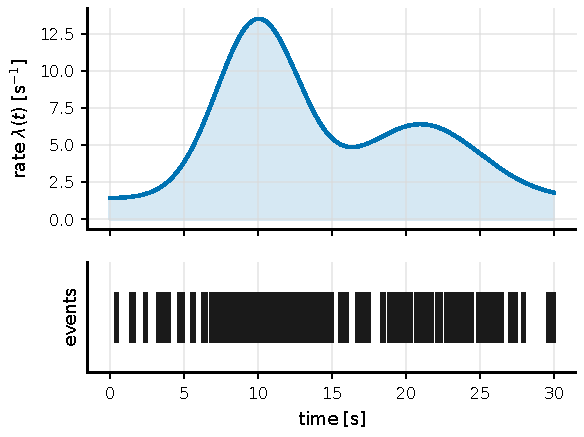
\includegraphics[width=0.72\linewidth]{figures/generated/chapter_07/ch07_poisson_likelihood.pdf}
\caption{非齐次 Poisson 过程的观测图像。上图是瞬时事件率 \(\lambda(t)\)，下图是从该率产生的一组事件时间。似然函数同时使用事件落在高率区域的事实和整段观测的积分率；只把事件重新分箱成一条光变曲线会丢失一部分时间信息，尤其在快速变化和不均匀曝光时更明显。}
\label{fig:ch07-poisson-likelihood}
\end{figure}

如果把事件先分进时间 bin，点过程似然退化为分箱 Poisson 似然：
\begin{equation}
  \ln L
  =
  \sum_i
  \left[
  d_i\ln m_i(\boldsymbol{\theta})
  -m_i(\boldsymbol{\theta})
  -\ln(d_i!)
  \right],
  \label{eq:ch07-binned-poisson}
\end{equation}
\begin{formulaexplain}
\(d_i\) 是第 \(i\) 个 bin 的观测计数，\(m_i\) 是模型计数。这个 Poisson 似然适合分箱后的光变、谱道或延迟直方图，并保留低计数的不对称统计。
\end{formulaexplain}
\(d_i\) 是第 \(i\) 个 bin 的观测计数，\(m_i\) 是模型预言计数，二者都无量纲。这个式子适合光变曲线、延迟直方图和谱道计数；当 \(d_i\gtrsim20\) 且模型远离边界时，常可近似为 Gaussian 似然。若背景、响应矩阵、吸收、时钟漂移或多个模型分量同时存在，似然比检验不一定服从名义上的 \(\chi^2\) 分布；新增分量强度被限制为非负时，零强度位于参数边界，显著性需要用模拟、后验预测检验或明确的模型证据校准 \citep{2002ApJ...571..545P}。

事件表还可以用自适应分段来描述慢变背景或爆发。Bayesian Blocks 把时间轴划成若干常率区间，对事件数据、binned counts 和带误差测量都给出相应的 fitness function；数据空隙通过 live time 进入，而不是被误认为无事件区间 \citep{2013ApJ...764..167S}。在实际管线中，这类方法很适合做质量监控、背景分段和暂现源候选筛选；最终物理参数仍应由明确的模型似然给出。

\Needspace{16\baselineskip}
\section{两路事件怎样给出相关峰}

两路事件表 \(a,b\) 的基本观测量是校正后的时间差：
\begin{equation}
  \tau_{ij}^{ab}
  =
  t_{j,b}^{\rm cal}
  -
  t_{i,a}^{\rm cal}
  -
  \Delta t_{\rm geo}^{ab}(t_i,\hat{\mathbf{s}})
  -
  \Delta t_{\rm inst}^{ab}(t_i).
  \label{eq:ch07-event-delay}
\end{equation}
\begin{formulaexplain}
\(\tau_{ij}^{ab}\) 是站点 \(a,b\) 两个事件的校正延迟；\(t^{\rm cal}\) 是标定时间；\(\Delta t_{\rm geo}\) 和 \(\Delta t_{\rm inst}\) 分别扣除几何和仪器延迟。它决定事件对落入哪个相关 bin。
\end{formulaexplain}
\(t_{i,a}^{\rm cal}\) 和 \(t_{j,b}^{\rm cal}\) 的单位是秒，\(\Delta t_{\rm geo}^{ab}\) 是几何延迟，\(\Delta t_{\rm inst}^{ab}\) 是两通道剩余仪器延迟。对 100 m 基线，几何延迟最大约 333 ns；对 1 km 基线是 \(3.3\,\mu{\rm s}\)。若时间 bin 为 4 ns，几何延迟只要错一个 bin 就会把相关峰移出零延迟；若仪器达到几十皮秒，地球自转导致的投影基线变化也要在短时间块内更新 \citep{2006MNRAS.369..655H,2006MNRAS.372.1549E,2018RNAAS...2....4K,2020NatAs...4.1164A}。

延迟 bin \(k\) 的事件对数为
\begin{equation}
  C_{ab,k}
  =
  \sum_{i\in a}\sum_{j\in b}
  S_iS_j\,
  \mathbf{1}
  \left[
  \tau_k-\frac{\Delta\tau}{2}
  \le
  \tau_{ij}^{ab}
  <
  \tau_k+\frac{\Delta\tau}{2}
  \right],
  \label{eq:ch07-pair-count}
\end{equation}
\begin{formulaexplain}
\(C_{ab,k}\) 是第 \(k\) 个延迟 bin 的事件对数；\(S_iS_j\) 给事件权重；指示函数只选择延迟落在 \(\tau_k\pm\Delta\tau/2\) 内的事件对。它是延迟直方图的基本计数。
\end{formulaexplain}
\(\Delta\tau\) 是延迟 bin 宽，单位秒；\(C_{ab,k}\) 无量纲。若两个通道独立且事件率在活时间内近似稳定，随机符合的期望为
\begin{equation}
  B_{ab,k}
  \simeq
  R_a R_b\,\Delta\tau\,T_{\rm live},
  \label{eq:ch07-accidental}
\end{equation}
\begin{formulaexplain}
\(B_{ab,k}\) 是随机符合背景；\(R_a,R_b\) 是两路平均事件率，\(\Delta\tau\) 是 bin 宽，\(T_{\rm live}\) 是活时间。它给出无天体相关时每个延迟 bin 应有的偶然事件对。
\end{formulaexplain}
\(R_a,R_b\) 的单位是 s\(^{-1}\)，\(T_{\rm live}\) 是扣除坏时间和死时间后的积分时间。典型强度干涉中 \(R_a\) 和 \(R_b\) 可在 \(10^6\)--\(10^8\,{\rm s^{-1}}\)，\(\Delta\tau\) 为 0.1--10 ns，\(T_{\rm live}\) 为分钟到夜级；因此 \(B_{ab,k}\) 可以很大，而天体相关只是这个背景上的 \(10^{-6}\) 到 \(10^{-4}\) 量级超额 \citep{1974iiia.book.....H,2020NatAs...4.1164A,2024MNRAS.529.4387A}。

归一化后的二阶相关估计量写成
\begin{equation}
  \widehat{g}^{(2)}_{ab}(\tau_k)
  =
  \frac{C_{ab,k}}{B_{ab,k}},
  \qquad
  \widehat{C}_{ab}(\tau_k)
  =
  \widehat{g}^{(2)}_{ab}(\tau_k)-1.
  \label{eq:ch07-g2-estimator}
\end{equation}
\begin{formulaexplain}
\(\widehat g^{(2)}\) 是归一化二阶相关估计；\(C_{ab,k}\) 是观测事件对数，\(B_{ab,k}\) 是随机背景；\(\widehat C_{ab}\) 是相对随机背景的超额。强度干涉信号就在这个超额里。
\end{formulaexplain}
\(\widehat{C}_{ab}\) 无量纲。若使用连续波形而不是离散事件，MAGIC-SII 采用 Pearson 相关
\begin{equation}
  \rho_{ab}(\tau_k)
  =
  \frac{\sum_n
  \left[x_a(t_n)-\bar{x}_a\right]
  \left[x_b(t_n+\tau_k)-\bar{x}_b\right]}
  {\sqrt{\sum_n\left[x_a(t_n)-\bar{x}_a\right]^2
  \sum_n\left[x_b(t_n)-\bar{x}_b\right]^2}},
  \label{eq:ch07-pearson}
\end{equation}
\begin{formulaexplain}
\(\rho_{ab}\) 是两路连续波形的 Pearson 相关；\(x_a,x_b\) 是采样电压或电流，\(\bar x\) 是平均值。它衡量去均值后的同步涨落，但还需背景和通量标定才变成 \(|V|^2\)。
\end{formulaexplain}
\(x_a\) 和 \(x_b\) 是数字化电压或电流样本。这个量在硬件里容易实时计算，但它包含恒星、夜天光和电子噪声的混合贡献，还要用直流电流、背景像素和零基线标定转换成 \(|V|^2\) \citep{2024MNRAS.529.4387A}。

\begin{figure}[tbp]
\centering
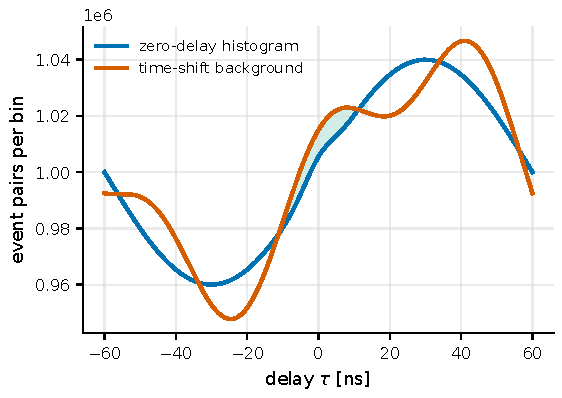
\includegraphics[width=0.72\linewidth]{figures/generated/chapter_07/ch07_time_shift_background.pdf}
\caption{时移背景估计的结构。蓝线是零延迟附近的事件对直方图，橙线是把一个通道整体平移到非物理延迟后得到的 accidental background。绿色区域表示中央相关峰相对时移背景的超额。这个方法可以保留慢变率、坏时间和背景结构，但平移量要远大于仪器响应宽度和天体相关宽度。}
\label{fig:ch07-time-shift-background}
\end{figure}

实际管线通常不用式 \eqref{eq:ch07-accidental} 直接归一化，而是用时间滑移、off-source、off-band 或错偏振估计 \(B_{ab,k}\)。时间滑移把通道 \(b\) 整体平移 \(\Delta T_{\rm shift}\)，要求 \(|\Delta T_{\rm shift}|\) 远大于相关峰宽，却小于背景和增益慢变时间。多个正负滑移可以给出背景均值和背景不确定度。off-source 适合夜天光和暗电流估计，off-band 适合谱线科学，错偏振适合寻找偏振串扰。VERITAS-SII 在 1 s 相关帧上剔除高频电子噪声和低 PMT 电流帧，再对几何延迟校正后的帧加权平均；MAGIC-SII 同时使用信号像素和背景像素的 DC 读数修正夜天光 \citep{2020NatAs...4.1164A,2024MNRAS.529.4387A}。

bin 宽 \(\Delta\tau\) 要和相关峰宽、时间戳量化和最终拟合方式一起选。若 \(\Delta\tau\) 远大于相关峰宽，峰高会被平均稀释；若它远小于时间戳量化和响应函数宽度，相邻 bin 会强相关，计算量也会上升。若最终只拟合峰面积，过细分箱不会增加总信息。对 VERITAS-SII，相关 lag 间隔为 4 ns，峰宽固定在约 4 ns；对 80 ps TDC 和几十皮秒探测器，bin 可以更细，但几何延迟、仪器响应和时钟残差也要同等精度 \citep{2020NatAs...4.1164A,2020RScI...91a3108W,2009A&A...508..531N}。

\section{相关器怎样在可承受时间内工作}

直接双循环计算式 \eqref{eq:ch07-pair-count} 的复杂度是 \(O(N_aN_b)\)。若两路各有 \(10^9\) 个事件，全量比较需要 \(10^{18}\) 次差分，不可能作为常规分析。排序窗口算法先按时间排序，只在 \(|t_{j,b}-t_{i,a}|\le W\) 的窗口内找事件对：
\begin{equation}
  N_{\rm pair}^{\rm win}
  \simeq
  2W\,R_b\,N_a .
  \label{eq:ch07-window-pairs}
\end{equation}
\begin{formulaexplain}
\(N_{\rm pair}^{\rm win}\) 是窗口算法需要检查的候选事件对数；\(W\) 是延迟窗口半宽，\(R_b\) 是第二路事件率，\(N_a\) 是第一路事件数。有限窗口把复杂度从全量双循环大幅降下来。
\end{formulaexplain}
\(W\) 是最大延迟窗口半宽，单位秒。如果 \(W=100\,{\rm ns}\)、\(R_b=10^6\,{\rm s^{-1}}\)、\(N_a=10^9\)，候选对约 \(2\times10^8\)，比全量双循环少十个数量级。这个算法适合稀疏事件表，也适合保留每个事件的波长和偏振标签。

若已经把事件或电压流放进均匀时间 bin，可用 FFT 计算互相关：
\begin{equation}
  c_{ab}[k]
  =
  \mathcal{F}^{-1}
  \left[
  \mathcal{F}\{x_a[n]\}^{*}
  \mathcal{F}\{x_b[n]\}
  \right]_k .
  \label{eq:ch07-fft-correlation}
\end{equation}
\begin{formulaexplain}
\(c_{ab}[k]\) 是离散互相关；\(\mathcal F\) 和 \(\mathcal F^{-1}\) 是 Fourier 变换与反变换；星号表示复共轭。FFT 把时域互相关改写成频域乘法，适合均匀采样数据。
\end{formulaexplain}
\(x_a[n]\) 和 \(x_b[n]\) 是时间序列，\(\mathcal{F}\) 是离散 Fourier 变换。FFT 方法的复杂度约 \(O(M\log M)\)，\(M\) 是时间 bin 数；它适合连续采样和固定 bin 的高速相关，但一旦分箱完成，低于 bin 宽的时间信息就不能恢复。VERITAS-SII 把连续 PMT 信号流到磁盘后用 FPGA 离线相关；MAGIC-SII 用 GPU 在观测时实时计算四通道所有成对相关；多通道 TCSPC 输出按时间排序的事件流，便于离线构造任意延迟和通道选择 \citep{2020NatAs...4.1164A,2024MNRAS.529.4387A,2020RScI...91a3108W}。

\begin{figure}[tbp]
\centering
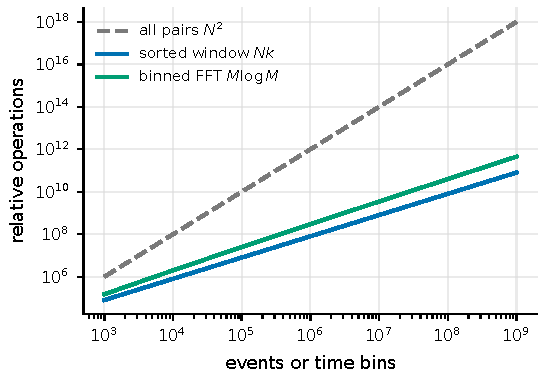
\includegraphics[width=0.72\linewidth]{figures/generated/chapter_07/ch07_correlator_scaling.pdf}
\caption{三类相关计算的操作数标度。全量事件对双循环随 \(N^2\) 增长，只适合小样本或教学检验；排序窗口算法只比较有限延迟内的事件对，接近线性增长；均匀分箱后的 FFT 相关随 \(M\log M\) 增长，适合连续采样或实时质量监控。实际速度还取决于内存带宽、I/O、GPU/FPGA 数据布局和质量标记筛选。}
\label{fig:ch07-correlator-scaling}
\end{figure}

算法选择会反过来影响科学量。排序窗口保留每个事件的全部标签，适合后验重新筛选；FFT 相关速度快，适合固定通道和固定时间 bin；实时 FPGA/GPU 相关可以在观测中发现时钟跳变、电子串扰和云导致的通量突变，但通常只保存压缩后的相关产品。对长期归档，原始事件或原始波形、标定事件、相关产品最好同时保存；FITS BINTABLE 适合事件归档，HDF5/Parquet 适合列式大数据分析，Astropy 可处理 FITS、时间和坐标元数据 \citep{2010A&A...524A..42P,2013A&A...558A..33A,2018AJ....156..123A}。

\section{误差为什么不是一串独立误差棒}

若 \(C_{ab,k}\) 和 \(B_{ab,k}\) 都是独立 Poisson 计数，且背景由 \(M\) 个等权时间滑移估计，则中央超额的近似方差为
\begin{equation}
  \operatorname{Var}
  \left[
  C_{ab,k}-\widehat{B}_{ab,k}
  \right]
  \simeq
  C_{ab,k}
  +
  \frac{1}{M}B_{ab,k}.
  \label{eq:ch07-excess-variance}
\end{equation}
\begin{formulaexplain}
\(\operatorname{Var}\) 是中央超额的方差；\(C_{ab,k}\) 给信号窗口的 Poisson 噪声，\(B_{ab,k}/M\) 给 \(M\) 个滑移背景平均后的不确定度。它是独立计数近似下的误差预算。
\end{formulaexplain}
这个近似只在事件独立、滑移背景互不重叠且率稳定时成立。真实数据里，相邻延迟 bin 共享事件，多个基线共享同一望远镜，多个波长通道共享天气和增益，多个模型点共享零基线归一化，因此误差通常不是对角的。

完整数据向量可以写为
\begin{equation}
  \mathbf{d}
  =
  \left(
  \widehat{|V|^2}_{1},
  \widehat{|V|^2}_{2},
  \ldots,
  \widehat{|V|^2}_{N_d}
  \right),
  \qquad
  \Sigma_{ij}
  =
  \left\langle
  (d_i-\mu_i)(d_j-\mu_j)
  \right\rangle .
  \label{eq:ch07-covariance}
\end{equation}
\begin{formulaexplain}
\(\mathbf d\) 是相关产品数据向量；\(d_i\) 是第 \(i\) 个 \(|V|^2\) 数据点，\(\mu_i\) 是其均值；\(\Sigma_{ij}\) 是协方差。非对角项记录共享望远镜、背景或标定带来的相关误差。
\end{formulaexplain}
\(\Sigma_{ij}\) 的单位是数据量单位的乘积；若 \(d_i\) 是无量纲 \(|V|^2\)，\(\Sigma\) 也无量纲。协方差可由解析误差传播、时间块 bootstrap、jackknife、时移背景集合或端到端注入仿真估计。时间块长度要长于相关峰宽、电子噪声相关时间和指向/天气短时波动；对夜级数据，常用 10 s 到数分钟的块来测试误差是否随 \(T^{-1/2}\) 收敛。MAGIC-SII 把电子带宽、光学带宽、DC 读出增益、背景扣除和残余电子噪声列为系统项，并通过改变 \(|V|^2\) 数据点的极端方向估计角直径系统误差 \citep{2024MNRAS.529.4387A}。

\begin{figure}[tbp]
\centering
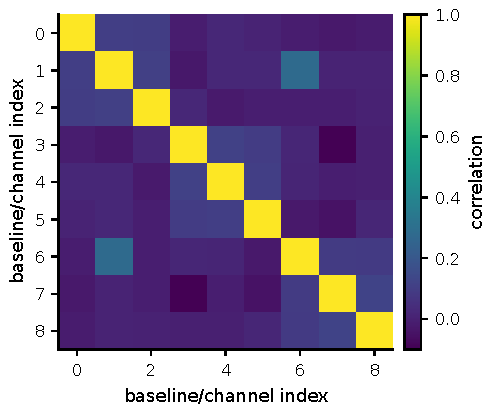
\includegraphics[width=0.66\linewidth]{figures/generated/chapter_07/ch07_covariance_matrix.pdf}
\caption{多基线或多通道结果的协方差矩阵示意。对角项是单个数据点方差，邻近块来自同一时间段或同一望远镜共享的噪声，远离对角线的结构可能来自共同背景估计、零基线归一化或电子串扰。模型拟合若只使用对角误差，会把有效独立信息量估得过高。}
\label{fig:ch07-covariance-matrix}
\end{figure}

空检验要和主分析使用同一套选择函数和权重。常用检验包括：把一个通道平移到非物理延迟；交换正负几何延迟；使用两个不应相关的偏振或波长通道；把目标外天空作为背景；把望远镜对分成不同时间块；把单个望远镜或单夜数据逐一剔除；在真实事件表中注入已知相关峰并检查能否无偏恢复。若主信号只在某个选择阈值下出现，而在相邻阈值、错延迟或 jackknife 中消失，它更可能是管线选择或仪器状态的结果，而不是天体相关。

\section{怎样从相关产品得到物理参数}

相关函数估计完成后，常见模型是把角直径、双星分离、亮度比、环半径或喷流参数映射到平方可见度：
\begin{equation}
  \mathbf{m}(\boldsymbol{\theta})
  =
  \left[
  |V(\mathbf{u}_1,\lambda_1\mid\boldsymbol{\theta})|^2,
  \ldots,
  |V(\mathbf{u}_{N_d},\lambda_{N_d}\mid\boldsymbol{\theta})|^2
  \right].
  \label{eq:ch07-model-vector}
\end{equation}
\begin{formulaexplain}
\(\mathbf m(\boldsymbol\theta)\) 是物理模型预言的数据向量；每一项是在对应空间频率 \(\mathbf u_i\) 和波长 \(\lambda_i\) 处的 \(|V|^2\)。它把角直径、双星参数或结构参数映射到观测量。
\end{formulaexplain}
\(\mathbf{u}=\mathbf{B}_\perp/\lambda\) 是空间频率，单位 rad\(^{-1}\) 或以波长为单位的投影基线；\(\boldsymbol{\theta}\) 是物理参数。若 \(\mathbf{d}\) 已经是近似 Gaussian 的相关产品，似然可写为
\begin{equation}
  -2\ln L
  =
  \left[\mathbf{d}-\mathbf{m}(\boldsymbol{\theta})\right]^T
  \Sigma^{-1}
  \left[\mathbf{d}-\mathbf{m}(\boldsymbol{\theta})\right]
  +\ln |\Sigma| + {\rm const}.
  \label{eq:ch07-gaussian-likelihood}
\end{equation}
\begin{formulaexplain}
\(\mathbf d-\mathbf m\) 是数据和模型残差；\(\Sigma^{-1}\) 按协方差加权；\(\ln|\Sigma|\) 是协方差归一化项。它是带相关误差的数据产品常用 Gaussian 似然。
\end{formulaexplain}
如果直接拟合原始计数或低计数延迟 bin，应回到式 \eqref{eq:ch07-binned-poisson}。VERITAS-SII 用均匀圆盘和边缘昏暗模型拟合 \(|g^{(1)}|^2\) 随投影基线的变化；MAGIC-SII 把 Pearson 相关经通量和背景校准后得到 \(|V|^2\)，再拟合恒星角直径和系统误差 \citep{2020NatAs...4.1164A,2024MNRAS.529.4387A,1967MNRAS.137..375H}。

观测设计阶段常用 Fisher 矩阵估计参数误差：
\begin{equation}
  F_{\alpha\beta}
  =
  \frac{\partial \mathbf{m}^T}{\partial \theta_\alpha}
  \Sigma^{-1}
  \frac{\partial \mathbf{m}}{\partial \theta_\beta},
  \qquad
  \operatorname{Cov}(\theta_\alpha,\theta_\beta)
  \gtrsim
  (F^{-1})_{\alpha\beta}.
  \label{eq:ch07-fisher}
\end{equation}
\begin{formulaexplain}
\(F_{\alpha\beta}\) 是 Fisher 信息矩阵；导数描述模型对参数的敏感度，\(\Sigma^{-1}\) 给误差权重；\(F^{-1}\) 近似给参数协方差下界。它用于观测规划和高信噪比误差估计。
\end{formulaexplain}
\(F_{\alpha\beta}\) 的单位是 \(\theta_\alpha^{-1}\theta_\beta^{-1}\)。若误差只由独立光子统计决定，信息量通常随有效光子数近似线性增加，参数误差随 \(N_{\rm eff}^{-1/2}\) 降低；一旦电子带宽、背景扣除、零基线归一化或通道增益给出系统地板，继续积分只会让误差趋近地板。Fisher 矩阵来自局部二次近似，适合观测规划和高信噪比近似；多峰后验、非线性退化或参数边界需要 MCMC、nested sampling 或端到端模拟 \citep{1925PCPS...22..700F,2013PASP..125..306F,2009MNRAS.398.1601F}。

\begin{figure}[tbp]
\centering
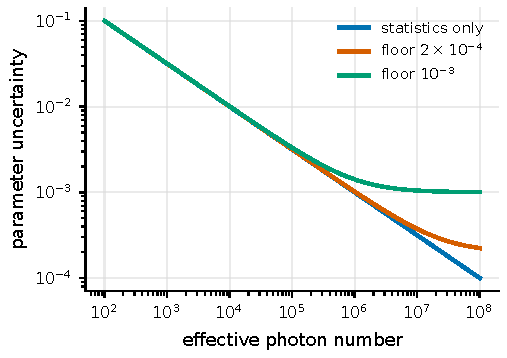
\includegraphics[width=0.70\linewidth]{figures/generated/chapter_07/ch07_fisher_scaling.pdf}
\caption{参数误差随有效光子数增加的标度。蓝线是纯统计 \(N_{\rm eff}^{-1/2}\) 下降；橙线和绿线加入不同系统误差地板后，长时间积分不再改善最终误差。观测计划应把积分时间、目标亮度、基线覆盖和系统标定放在同一个误差预算里。}
\label{fig:ch07-fisher-scaling}
\end{figure}

贝叶斯后验写成
\begin{equation}
  p(\boldsymbol{\theta}\mid\mathcal{D},M)
  =
  \frac{
  L(\mathcal{D}\mid\boldsymbol{\theta},M)\,
  \pi(\boldsymbol{\theta}\mid M)}
  {Z_M},
  \qquad
  Z_M=
  \int
  L\,\pi\,d\boldsymbol{\theta}.
  \label{eq:ch07-posterior}
\end{equation}
\begin{formulaexplain}
\(p(\boldsymbol\theta\mid\mathcal D,M)\) 是模型 \(M\) 下的参数后验；\(L\) 是似然，\(\pi\) 是先验，\(Z_M\) 是证据。它把数据约束和外部物理先验合成完整的不确定度描述。
\end{formulaexplain}
\(\pi\) 是先验，\(Z_M\) 是模型证据。先验可以来自距离、光谱型、已有角直径、双星轨道、爆发时间或物理边界；它需要写清楚，因为强度干涉常只测 \(|V|^2\)，缺少相位会让镜像、亮度比和位置角出现退化。emcee 适合中等维度后验采样，MultiNest 适合多峰后验和模型证据估计；二者都不能替代物理检查，链的自相关时间、接受率、先验体积和模拟注入恢复都要报告 \citep{2013PASP..125..306F,2009MNRAS.398.1601F,1992ApJ...398..146G}。


\chapter{量子估计、Rayleigh 限制和亚分辨信息}
\label{chap:08}

\begin{chapteropening}
Rayleigh 判据给出的是一个成像判据：两个 Airy 斑的主峰是否能在像面上分成两个峰。天文观测中更常见的问题是估计问题：给定一批光子、一个点扩散函数和一个源模型，双星角分离、恒星角直径或亮度矩的误差能小到什么程度。量子估计理论把这个问题写成光场态和测量之间的信息匹配；对弱热光源，直接成像会在亚 Rayleigh 区域丢失一部分分离信息，空间模式测量则可以保留关于分离和尺度的 Fisher 信息 \citep{1925PCPS...22..700F,1969JSP.....1..231H,2000PhRvL..85.3789K,2016PhRvX...6c1033T,2016OExpr..24.3684N,2017NJPh...19b3054T}。
\end{chapteropening}

\section{Rayleigh 判据为什么不是估计极限}

设望远镜口径为 \(D\)，波长为 \(\lambda\)。圆孔衍射的第一个零点在
\begin{equation}
  \theta_{\rm R}=1.22\,\frac{\lambda}{D}
  \label{eq:ch08-rayleigh}
\end{equation}
\begin{formulaexplain}
\(\theta_{\rm R}\) 是 Rayleigh 角尺度；\(\lambda\) 是波长，\(D\) 是口径，系数 1.22 来自圆孔 Airy 斑第一个零点。它给出像面分峰判据，而不是参数估计的最终极限。
\end{formulaexplain}
处。这里 \(\theta_{\rm R}\) 的单位是弧度；乘以 \(206265\times10^3\) 可换成毫角秒。一个 \(D=8~{\rm m}\) 的望远镜在 \(\lambda=500~{\rm nm}\) 时有 \(\theta_{\rm R}\simeq 15.7~{\rm mas}\)，在 \(1.6~\mu{\rm m}\) 时约为 \(50~{\rm mas}\)；一个 \(30~{\rm m}\) 望远镜在 \(500~{\rm nm}\) 时约为 \(4.2~{\rm mas}\)。真实点扩散函数由孔径遮挡、分段镜、像差、自适应光学校正和大气残差共同决定。为了看清解析结构，先采用一维高斯点扩散函数：
\begin{equation}
  h(x)=\frac{1}{\sqrt{2\pi}\sigma}
       \exp\!\left(-\frac{x^2}{2\sigma^2}\right),
  \label{eq:ch08-gaussian-psf}
\end{equation}
\begin{formulaexplain}
\(h(x)\) 是归一化点扩散函数；\(x\) 是像面或角坐标，\(\sigma\) 是宽度。这个高斯模型把真实 PSF 简化成一个可解析的响应核，方便看清分离信息怎样进入数据。
\end{formulaexplain}
其中 \(x\) 是焦平面坐标或等效角坐标，\(\sigma\) 是同一坐标下的点扩散函数宽度。若用角坐标，\(\sigma_\theta\) 的典型量级约为 \(0.4\lambda/D\) 到 \(0.5\lambda/D\)，具体数值要由实测 PSF 或注入源标定给出。

两个等亮、互不相干点源的角分离为 \(s\)，质心放在零点。直接成像记录的是像面光子位置 \(x_i\)，其单光子概率密度为
\begin{equation}
  p(x|s)=\frac{1}{2}h\!\left(x-\frac{s}{2}\right)
        +\frac{1}{2}h\!\left(x+\frac{s}{2}\right).
  \label{eq:ch08-direct-probability}
\end{equation}
\begin{formulaexplain}
\(p(x|s)\) 是给定分离 \(s\) 时单个光子落在 \(x\) 的概率密度；两个 \(h\) 分别来自质心两侧的点源，系数 \(1/2\) 表示等亮。直接成像只看到两个 PSF 的混合。
\end{formulaexplain}
左边的 \(p(x|s)\) 在数据中由归一化图像、事件位置直方图或 PSF 拟合得到，单位是角度的倒数。右边的 \(s\) 和 \(\sigma\) 应使用同一单位。式 \eqref{eq:ch08-direct-probability} 假设两个源等亮、谱形相同、PSF 对两个源相同、背景已扣除或另行建模；若亮度比未知，需要把通量比也放进参数向量。

现在问题变清楚了：Rayleigh 判据问的是像面曲线是否出现两个峰，而估计问题问的是 \(p(x|s)\) 随 \(s\) 改变得有多快。直接图像在 \(s\ll\sigma\) 时几乎不变。把式 \eqref{eq:ch08-direct-probability} 中的两个偏移 PSF 展开，
\[
  h\!\left(x\pm\frac{s}{2}\right)
  =h(x)\pm\frac{s}{2}h'(x)+\frac{s^2}{8}h''(x)+\mathcal{O}(s^3),
\]
放回平均后，一阶项相互抵消，
\[
  p(x|s)=h(x)+\frac{s^2}{8}h''(x)+\mathcal{O}(s^4).
\]
也就是说，双源分离首先表现为 PSF 的二阶展宽，而不是峰位的一阶移动。于是“看不出两个峰”并不等价于“没有任何信息”，但直接像素测量得到的信息确实会迅速下降。对高斯 PSF，分离参数的单光子 Fisher 信息在小分离极限满足
\begin{equation}
  F_{ss}^{\rm direct}\simeq \frac{s^2}{8\sigma^4},
  \qquad s\ll\sigma .
  \label{eq:ch08-direct-small-s}
\end{equation}
\begin{formulaexplain}
\(F_{ss}^{\rm direct}\) 是直接成像对分离 \(s\) 的单光子 Fisher 信息；小分离时它正比于 \(s^2\)。因此两源越接近，像素数据对分离的一阶灵敏度越弱。
\end{formulaexplain}
这里 \(F_{ss}^{\rm direct}\) 的单位是角度的 \(-2\) 次方。若把参数写成无量纲的 \(q=s/\sigma\)，则 \(F_{qq}^{\rm direct}\simeq q^2/8\)。这个二次下降就是 Rayleigh curse：光子数增加当然会降低误差，但在固定光子数下，源越接近，直接成像对分离越不敏感 \citep{2016PhRvX...6c1033T,2018Optic...5.1177P}。

\begin{figure}[tbp]
\centering
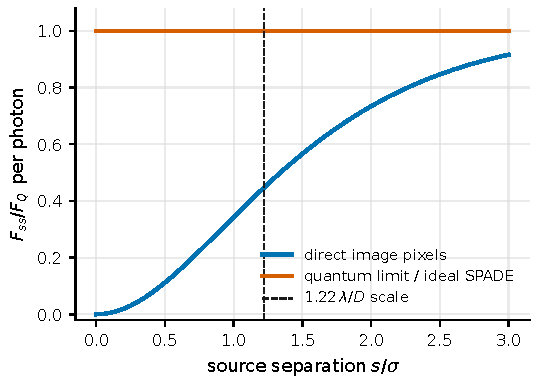
\includegraphics[width=0.82\linewidth]{figures/generated/chapter_08/ch08_rayleigh_information.pdf}
\caption{两个等亮不相干高斯点源的分离信息。蓝线是由像面概率密度 \(p(x|s)\) 数值积分得到的直接成像 Fisher 信息，并按量子 Fisher 信息归一化；橙线表示理想空间模式测量可达到的量子极限。小分离时直接图像的形状变化为二阶小量，因此 \(F_{ss}^{\rm direct}\) 向零下降，而模式测量仍能保留有限信息。虚线标出常用的 Rayleigh 角尺度位置。}
\label{fig:chapter-08-rayleigh-information}
\end{figure}

估计问题和检测问题要分开。若问题是“一个源还是两个源”，模型维数会改变，分离 \(s=0\) 又位在参数空间边界，常规似然比近似未必可靠；若已经接受双源模型，问题才是估计 \(s\)、质心、亮度比和颜色。亚分辨测量依赖给定的参数化模型，用更合适的测量读出已经存在于光场中的信息。对真实天体，模型通常还包括有限角直径、伴星亮度比、谱带差异、偏振、时间变化和背景星污染，这些都会把单参数下界变成多参数协方差问题。

\section{Fisher 信息在比较什么}

一次观测得到 \(N_\gamma\) 个可用于估计的源光子。若背景、坏像素和选择函数已经写进概率密度，直接成像的似然函数可写为
\begin{equation}
  \ln \mathcal{L}(s)=\sum_{i=1}^{N_\gamma}\ln p(x_i|s),
  \label{eq:ch08-direct-likelihood}
\end{equation}
\begin{formulaexplain}
\(\ln\mathcal L(s)\) 是分离 \(s\) 的直接成像对数似然；\(x_i\) 是第 \(i\) 个光子位置，\(N_\gamma\) 是有效源光子数。它把所有光子位置对同一分离模型的支持相加。
\end{formulaexplain}
其中 \(x_i\) 是第 \(i\) 个光子的角位置或像素位置。对应的 Fisher 信息为
\begin{equation}
  F_{ss}=N_\gamma \int
  \frac{1}{p(x|s)}
  \left[\frac{\partial p(x|s)}{\partial s}\right]^2{\rm d}x .
  \label{eq:ch08-fisher-direct}
\end{equation}
\begin{formulaexplain}
\(F_{ss}\) 是总 Fisher 信息；导数 \(\partial p/\partial s\) 衡量分离改变时概率密度变化多快，\(1/p\) 给出统计权重。它把模型灵敏度和光子数合成误差下界。
\end{formulaexplain}
积分变量 \(x\) 的单位和 \(s\) 一致。\(N_\gamma\) 是通过孔径、曝光时间、谱带、总效率和数据选择后留下的源光子数；对于明亮恒星，毫秒到小时曝光可覆盖 \(10^6\) 到 \(10^{12}\) 量级，具体值取决于望远镜面积、滤光片宽度、探测器效率和是否把光分到多个模式或多个基线。若每个像素还有背景 \(b(x)\)，则 \(p\) 要替换成源加背景的归一化混合分布，背景比 \(N_{\rm bg}/N_\gamma\) 从暗场中的 \(\ll 0.01\) 到拥挤星场或强天空背景下的 \(>1\) 都可能出现。

任意无偏估计量 \(\hat{s}\) 的方差满足
\begin{equation}
  {\rm Var}(\hat{s})\ge \frac{1}{F_{ss}} .
  \label{eq:ch08-crb}
\end{equation}
\begin{formulaexplain}
\(\hat s\) 是分离估计量；\({\rm Var}(\hat s)\) 是它的方差。Cramér--Rao 下界说明 Fisher 信息越大，任何无偏估计能达到的最小统计误差越小。
\end{formulaexplain}
若同时估计多个参数 \(\boldsymbol{\theta}=(s,x_0,r,\sigma,b,\ldots)\)，标量下界要换成矩阵形式
\begin{equation}
  {\rm Cov}(\hat{\boldsymbol{\theta}})\succeq F^{-1},\qquad
  F_{\alpha\beta}=N_\gamma\int
  \frac{1}{p(x|\boldsymbol{\theta})}
  \frac{\partial p}{\partial\theta_\alpha}
  \frac{\partial p}{\partial\theta_\beta}\,{\rm d}x .
  \label{eq:ch08-fisher-matrix}
\end{equation}
\begin{formulaexplain}
\({\rm Cov}(\hat{\boldsymbol\theta})\) 是多参数协方差矩阵；\(F_{\alpha\beta}\) 比较参数 \(\theta_\alpha,\theta_\beta\) 对同一数据分布的影响。矩阵逆中的非对角项记录参数退化。
\end{formulaexplain}
\(F^{-1}\) 的非对角项描述退化。比如未知质心会和分离混合，未知亮度比会把一部分偶模式和奇模式信息重新分配，未知 PSF 宽度会把双星分离和普通展宽混在一起。实际报告误差时，通常需要给出统计协方差、PSF 标定误差、背景估计误差和模型误差，而不是只给一个 \(1/\sqrt{F_{ss}}\)。

这时“量子”二字的作用很具体：它不是说望远镜绕过了衍射，而是把测量方式也放进优化问题。经典 Fisher 信息先固定测量，例如像素计数，然后问这些数据对参数有多少灵敏度。量子 Fisher 信息则把“像素测量”替换成“所有量子力学允许的测量”，问同一束光在原则上最多能携带多少可读出的参数信息。

第 \ref{chap:03} 章式 \eqref{eq:ch03-weak-thermal} 已经把弱热光写成真空项加少量一光子项：每个相干时间模式中的平均光子数为 \(\epsilon\ll1\)，大多数时间窗没有点击；没有点击的时间窗不携带角分离信息，真正进入估计的是被探测到的一光子空间模式。两个等亮不相干点源的一光子部分可写成
\begin{equation}
  \rho_1(s)=\frac{1}{2}
  \left|\psi_{+s/2}\right\rangle\left\langle\psi_{+s/2}\right|
  +\frac{1}{2}
  \left|\psi_{-s/2}\right\rangle\left\langle\psi_{-s/2}\right| ,
  \label{eq:ch08-one-photon-state}
\end{equation}
\begin{formulaexplain}
\(\rho_1(s)\) 是探测到一个光子时的空间模式密度矩阵；\(|\psi_{\pm s/2}\rangle\) 是两个源经过望远镜后的场模式。非相干等亮双源表现为两个单光子模式的概率混合。
\end{formulaexplain}
\Needspace{13\baselineskip}
其中 \(\psi_{\pm s/2}\) 是两个源通过望远镜和成像系统后的场振幅模式。对高斯振幅 PSF，在质心、亮度和 PSF 已知的理想情况下，分离的量子 Fisher 信息为
\begin{equation}
  F_{ss}^{Q}=N_\gamma\,\frac{1}{4\sigma^2}.
  \label{eq:ch08-qfi-gaussian}
\end{equation}
\begin{formulaexplain}
\(F_{ss}^{Q}\) 是所有允许测量中可达到的分离信息上限；\(N_\gamma\) 给出光子数增益，\(\sigma\) 给出模式宽度。它在 \(s\to0\) 时不消失，说明信息仍在光场中。
\end{formulaexplain}
它不随 \(s\to0\) 消失。式 \eqref{eq:ch08-qfi-gaussian} 中的 \(\sigma\) 是场模式对应的像面宽度；若用角坐标，它的单位是弧度。这个结果假设光学系统线性、损耗不随分离变化、两个源互不相干且等亮、中心位置已知，并且测量能接近最优空间模式投影 \citep{1969JSP.....1..231H,2016PhRvX...6c1033T,2016OExpr..24.3684N,2017PhRvA..95f3847A}。

\begin{figure}[tbp]
\centering
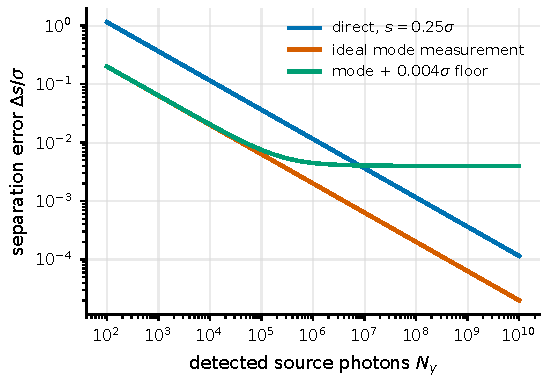
\includegraphics[width=0.82\linewidth]{figures/generated/chapter_08/ch08_cramer_rao_bound.pdf}
\caption{亚分辨双点源的 Cramér--Rao 分离误差。横轴为探测到的源光子数 \(N_\gamma\)，纵轴为 \(\Delta s/\sigma\)。在 \(s=0.25\sigma\) 的例子中，直接成像因 Fisher 信息已经很小，需要更多光子才能达到同样误差；理想模式测量按 \(N_\gamma^{-1/2}\) 下降。绿色曲线加入 \(0.004\sigma\) 的模式匹配系统误差后出现平台，表示继续增加光子数也不能消除标定误差。}
\label{fig:chapter-08-crb}
\end{figure}

量子下界不是自动可达的观测精度。若质心误差为 \(\delta x\)，第一阶模式会得到约 \(\delta x^2/(4\sigma^2)\) 的漏光；而双源分离信号本身在小分离时约为 \(s^2/(16\sigma^2)\)。因此当 \(\delta x\sim s/2\) 时，指向和质心标定已经和待测信号同量级。若 Strehl 比低、像差随时间变化、模式排序器串扰矩阵不稳定，或背景光没有同样的空间模式分布，式 \eqref{eq:ch08-qfi-gaussian} 给出的下界会被系统误差平台取代。实验相位板、PSF shaping 和 SPLICE 类测量表明，非理想但较简单的相位敏感测量也能缓和直接成像的二次信息损失，不过通常仍要靠可见度、串扰和对准误差来决定实际增益 \citep{2017PhRvL.118g0801T,2019NJPh...21i3010B,2018Optic...5.1177P}。

\section{空间模式测量怎样把小分离变成计数}

直接成像把每个光子投影到位置本征态，因此小分离只留下非常弱的形状展宽。空间模式测量换了一个问题：不先问光子落在哪个像素，而是先问它属于哪个正交空间模式。SPADE 把光场先分解到一组空间模式，再对每个模式计数。对于高斯 PSF，最自然的基底是 Hermite--Gaussian 模式。若质心已知且两个点源等亮，理想模式排序给出
\begin{equation}
  p_n=\exp(-Q)\frac{Q^n}{n!},\qquad
  Q=\frac{s^2}{16\sigma^2},
  \label{eq:ch08-spade-probability}
\end{equation}
\begin{formulaexplain}
\(p_n\) 是第 \(n\) 个 Hermite--Gaussian 模式的点击概率；\(Q\) 是由分离 \(s\) 和宽度 \(\sigma\) 构成的无量纲信号强度。SPADE 把分离转成低阶模式的计数分布。
\end{formulaexplain}
其中 \(p_n\) 是第 \(n\) 个 Hermite--Gaussian 模式的单光子概率。\(p_0\) 接近 1，表示绝大多数光仍在基模；\(p_1\simeq s^2/(16\sigma^2)\)，表示一个很小但可计数的奇模式漏出。这个漏出来自两个相互重叠的源模式在空间模式基底中的几何结构，是分离信号的一部分。对 \(N_\gamma\) 个光子，第一阶模式的期望计数为
\begin{equation}
  \langle n_1\rangle\simeq N_\gamma\,\frac{s^2}{16\sigma^2}.
  \label{eq:ch08-first-mode-count}
\end{equation}
\begin{formulaexplain}
\(\langle n_1\rangle\) 是第一阶模式的期望光子数；它等于总源光子数乘以小分离漏入该模式的概率。即使概率很小，大 \(N_\gamma\) 也能把它变成可测计数。
\end{formulaexplain}
例如 \(s=0.1\sigma\) 时，\(p_1\simeq6.25\times10^{-4}\)；若有效源光子数为 \(10^8\)，理想情况下第一阶模式中有约 \(6.3\times10^4\) 个光子。若通量只有 \(10^5\) 个光子，则期望计数约 63 个，暗计数、串扰和背景就会变成主要限制。

\begin{figure}[tbp]
\centering
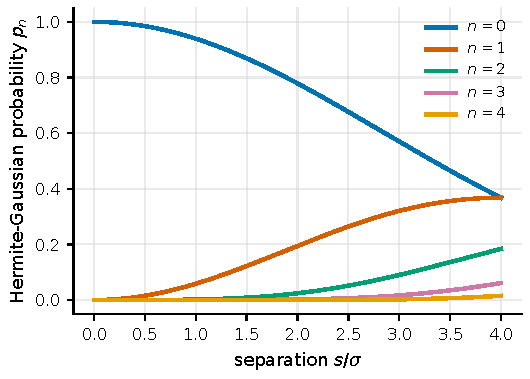
\includegraphics[width=0.82\linewidth]{figures/generated/chapter_08/ch08_spade_probabilities.pdf}
\caption{理想 Hermite--Gaussian 模式排序的模式概率。横轴是源分离 \(s/\sigma\)，纵轴是每个模式的单光子概率。小分离时 \(p_0\) 仍接近 1，但 \(p_1\) 和更高模式按 \(Q=s^2/(16\sigma^2)\) 的幂次增长；分离信息由这些低概率模式的计数携带。}
\label{fig:chapter-08-spade-probabilities}
\end{figure}

图像中的“看不出”可以同时出现在像面曲线和模式概率中：像面轮廓几乎重合，但低概率模式已经变成可测计数。若模式计数服从 Poisson 或 multinomial 统计，模式测量的 Fisher 信息为
\begin{equation}
  F_{ss}^{\rm mode}
  =N_\gamma\sum_n \frac{1}{p_n}
  \left(\frac{\partial p_n}{\partial s}\right)^2 .
  \label{eq:ch08-mode-fisher}
\end{equation}
\begin{formulaexplain}
\(F_{ss}^{\rm mode}\) 是模式计数给出的分离 Fisher 信息；求和覆盖所有空间模式。每一项用模式概率对 \(s\) 的变化率除以该模式的计数噪声，累加成总信息。
\end{formulaexplain}
在小分离极限，仅 \(n=1\) 模式就给出接近 \(N_\gamma/(4\sigma^2)\) 的信息。\(p_1\) 本身随 \(s^2\) 变小，但 \(\partial p_1/\partial s\) 也随 \(s\) 变小，两者在 Fisher 信息中相除后留下有限极限。模式测量由此避开 Rayleigh curse \citep{2016PhRvX...6c1033T,2017NJPh...19b3054T}。

\begin{figure}[tbp]
\centering
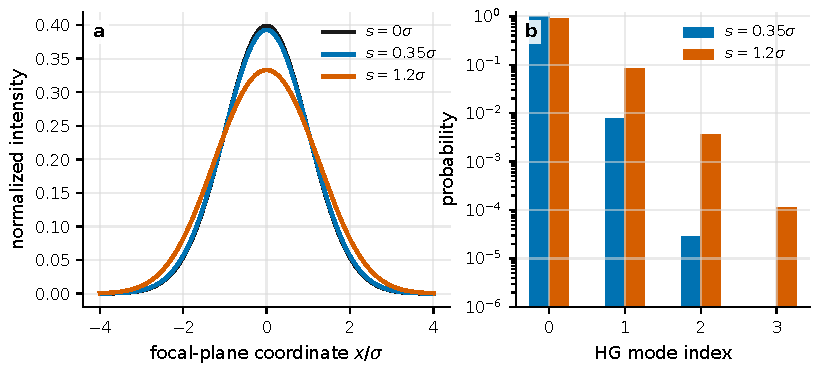
\includegraphics[width=0.92\linewidth]{figures/generated/chapter_08/ch08_direct_image_vs_modes.pdf}
\caption{同一双源模型在直接像面和模式输出中的表现。左图显示 \(s=0\)、\(0.35\sigma\) 和 \(1.2\sigma\) 的归一化像面强度；亚分辨分离时曲线差别主要表现为很弱的展宽。右图显示 \(s=0.35\sigma\) 和 \(1.2\sigma\) 的前四个 Hermite--Gaussian 模式概率；低阶非基模概率虽小，却把分离信息变成了模式计数。}
\label{fig:chapter-08-direct-vs-modes}
\end{figure}

天文实现还要处理二维分离、偏振、谱带和光学耦合。二维问题把 \(s\) 换成 \((s_x,s_y)\)，相应模式变成二维 Hermite--Gaussian 或与真实孔径匹配的正交模式；角分离的两个方向在圆对称 PSF 下有相同量级的 QFI，但非圆 PSF、分段镜和像差会引入方向依赖 \citep{2017PhRvA..95f3847A}。广义 SPADE 可估计亚衍射目标的二阶及更高空间矩，但高阶矩需要更高阶模式，光子数需求迅速上升，有限矩也不能唯一重建任意亮度分布 \citep{2017NJPh...19b3054T}。因此星对、近距离伴星、恒星形状和少参数亮度矩是更自然的应用；复杂盘面、喷流和星云需要把模式测量和常规成像、振幅干涉或强度干涉联合起来。

部分相干性会改变模式概率。Larson 和 Saleh 讨论了部分相干源中 Rayleigh curse 重新出现的条件；Tsang 和 Nair 随后指出，对弱热光和正确的 SPADE Fisher 计算，只要不是完全正相关的退化情形，模式测量仍可避免小分离信息完全消失 \citep{2018Optic...5.1382L,2019Optic...6..400T}。在天文学里要特别区分两件事：源面上两个辐射区域是否独立发光，以及传播到望远镜后由 van Cittert--Zernike 定理产生的空间相干。后者正是一阶或二阶干涉测量的目标，不应简单等同于源本身的相干发射。

\section{强度干涉怎样把角尺度写进长基线数据}

前一节讨论的是单孔径或相干合束后的空间模式测量。长基线阵列把同一个估计问题放到 Fourier 平面：不同望远镜对采样不同空间频率，数据约束来自可见度随基线的变化。这里的“亚分辨”不是从单个 Airy 斑里读出两个峰，而是在长基线上测量源亮度分布的 Fourier 模长。

强度干涉不测一阶场相位，而测不同望远镜光强涨落的相关。理想热光下，零延迟二阶相关给出
\begin{equation}
  g_{ij}^{(2)}(0)-1 = |\gamma_{ij}|^2,
  \label{eq:ch08-hbt-g2}
\end{equation}
\begin{formulaexplain}
\(g_{ij}^{(2)}(0)\) 是两台望远镜零延迟二阶相关；\(\gamma_{ij}\) 是归一化复相干度。热光 HBT 关系说明强度涨落相关直接给出可见度模平方。
\end{formulaexplain}
其中 \(\gamma_{ij}\) 是望远镜 \(i,j\) 之间的复相干度，等于归一化一阶可见度 \(V(u,v)\)。在有限时间 bin、有限光谱带宽和探测器响应下，实测对比度会被相干时间与电子时间分辨率的比值稀释；分析通常直接拟合校准后的 \(|V|^2\) 和它的协方差。HBT 实验和 Narrabri 强度干涉仪正是用这种方式测量恒星角直径，现代 Cherenkov 望远镜阵列则把大收集面积和数字相关器带入同一问题 \citep{1956Natur.177...27B,1956Natur.178.1046H,1957RSPSA.242..300B,1974iiia.book.....H,1974MNRAS.167..121H,1974MNRAS.167..475H,2008AIPC..984..205L,2013APh....43..331D,2015NatCo...6.6852D,2020NatAs...4.1164A,2024MNRAS.529.4387A}。

若观测量是若干基线和谱道上的
\begin{equation}
  d_k=|V(u_k,v_k;\boldsymbol{\theta})|^2+\eta_k ,
  \label{eq:ch08-sii-data}
\end{equation}
\begin{formulaexplain}
\(d_k\) 是第 \(k\) 个基线/时间/谱道上的平方可见度数据；\(V\) 是模型可见度，\(\boldsymbol\theta\) 是源参数，\(\eta_k\) 是噪声。强度干涉把角结构写进 \(|V|^2\) 的基线变化中。
\end{formulaexplain}
其中 \(k\) 标记基线、时间、谱道或偏振通道，\(\eta_k\) 是噪声项，则参数 \(\theta_\alpha\) 的 Fisher 矩阵可写成
\begin{equation}
  F_{\alpha\beta}^{\rm SII}
  =\sum_{k,l}
  \frac{\partial |V_k|^2}{\partial\theta_\alpha}
  C^{-1}_{kl}
  \frac{\partial |V_l|^2}{\partial\theta_\beta}.
  \label{eq:ch08-sii-fisher}
\end{equation}
\begin{formulaexplain}
\(F_{\alpha\beta}^{\rm SII}\) 是强度干涉数据的 Fisher 矩阵；\(C^{-1}_{kl}\) 按数据协方差给权重。可见度模平方对参数变化越陡、误差越小，对应参数信息越多。
\end{formulaexplain}
\(C_{kl}\) 是 \(|V|^2\) 测量误差协方差，可由时间移位背景、空基线、夜间重复观测或注入模拟估计。若误差近似独立，式 \eqref{eq:ch08-sii-fisher} 退化为每个数据点的斜率平方除以方差。对均匀圆盘恒星，
\begin{equation}
  V(x)=\frac{2J_1(x)}{x},\qquad
  x=\pi B\theta_\star/\lambda ,
  \label{eq:ch08-uniform-disk-visibility}
\end{equation}
\begin{formulaexplain}
\(V(x)\) 是均匀圆盘的可见度；\(J_1\) 是一阶 Bessel 函数，\(B\) 是投影基线，\(\theta_\star\) 是角直径。基线通过 \(x\) 扫描圆盘亮度分布的 Fourier 模长。
\end{formulaexplain}
\(B\) 是投影基线，\(\theta_\star\) 是角直径。对 \(\theta_\star\) 最有用的基线通常落在 \(|V|^2\) 斜率大的区域；短基线平台上模型变化太小，极长基线上信号又容易被系统误差压住。

\begin{figure}[tbp]
\centering
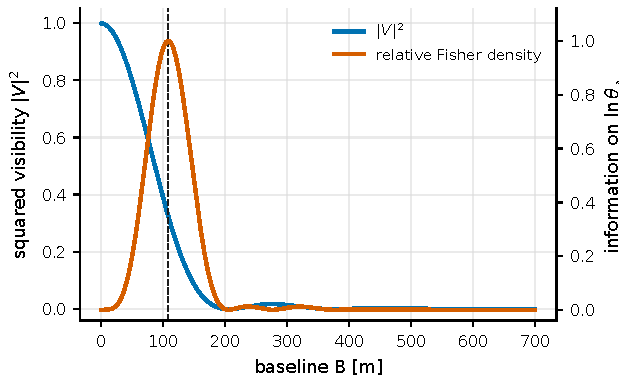
\includegraphics[width=0.82\linewidth]{figures/generated/chapter_08/ch08_visibility_fisher_design.pdf}
\caption{强度干涉中基线选择和参数信息的关系。蓝线为 \(\lambda=450~{\rm nm}\)、\(\theta_\star=0.55~{\rm mas}\) 均匀圆盘模型的平方可见度；橙线为按 \(\partial |V|^2/\partial\ln\theta_\star\) 计算并归一化的 Fisher 权重。最有用的基线位在可见度快速下降处，单纯增加或缩短基线都不会自动增加角直径信息。}
\label{fig:chapter-08-sii-fisher}
\end{figure}

强度干涉的代价是相位缺失。\(|V|^2\) 对整体平移不敏感，也会产生镜像和中心对称退化；二元星的方向、亮斑位置和非对称盘面结构往往需要地球自转覆盖、多波长信息、先验模型或三阶相关来缓解。它的优势是对大气相位扰动不敏感，望远镜之间只需电子连接，不必保持光学相干。现代时间标记器和高速相关器可以处理许多通道，但可用 Fisher 信息仍受光子率、电子带宽、背景、时间同步、基线覆盖和系统协方差限制 \citep{2017MNRAS.472.4126G,2020RScI...91a3108W,2020NatAs...4.1164A,2024MNRAS.529.4387A}。

\section{天文应用中怎样避免误读量子极限}

模式测量和强度干涉面对的是不同的工程瓶颈。SPADE、SLIVER 和相位敏感测量通常要求单孔径或相干组合后的稳定波前，适合把目标光耦合进光纤模式、集成光学芯片或自由空间模式排序器。自适应光学把入射光尽量压到可控的少数空间模式中；Strehl 比、非共路像差、色散和偏振串扰都会进入模式响应矩阵。强度干涉接受大气相位随机化，用大收集面积和长基线换取 \(|V|^2\) 信息，更适合亮热星、快速旋转星、双星和角直径测量。

一套可用于科学结果的亚分辨估计需要同时交代光子预算、角尺度、测量矩阵、模型边界和误差拆分。光子预算包括目标星等、谱带、总效率、曝光时间和有效 \(N_\gamma\)；角尺度包括 \(\lambda/D\)、PSF 宽度 \(\sigma_\theta\)、候选分离 \(s\) 或角直径 \(\theta_\star\)。测量矩阵可以是像素响应、模式串扰、\(|V|^2\) 协方差或时间相关背景。模型边界要说明等亮双源、未知亮度比、有限圆盘、部分相干、背景星和时间变化怎样改变 Fisher 矩阵。误差拆分则检查统计项是否按 \(N_\gamma^{-1/2}\) 下降；若误差不再下降，通常是对准、PSF、背景、相关器或模型误差进入平台。

贝叶斯采样和证据比较常用于把这些边界放入最终推断。直接成像、模式计数和强度干涉数据可以共享同一个参数向量，并用联合似然相乘；若要比较单源和双源模型，需要用模拟校准、后验预测检验或证据，而不是简单套用高斯近似。对亚分辨问题，先验会直接改变可识别参数空间：已知轨道、颜色、光谱型、距离、伴星亮度比或恒星演化模型都能改变最终约束 \citep{2009MNRAS.398.1601F,2013PASP..125..306F}。


\part[天体光源的量子语言]{天体光源的量子语言}
\chapter{天体辐射机制的量子语言}
\label{chap:09}

\begin{chapteropening}
同一个平均谱可以来自不同的光场。热辐射、自由自由辐射、同步辐射、逆康普顿散射、maser 和曲率辐射都能写出 \(I_\nu\)，但它们在相干时间、偏振、亮温、光子聚束和跨频相关上并不相同。把辐射机制写成光子统计问题后，谱指数和光变曲线会自然扩展为 \(g^{(2)}(\tau)\)、偏振分辨相关、频率通道之间的联合概率和事件到达时间分布 \citep{1963PhRv..130.2529G,1963PhRv..131.2766G,1995ocqo.book.....M,1956Natur.177...27B,2017MNRAS.472.4126G}。
\end{chapteropening}

\section{为什么平均谱不够}

辐射机制的传统入口是比强度 \(I_\nu\)，也就是单位时间、单位面积、单位频率、单位立体角内的辐射能流。若源在天空上的立体角为 \(\Omega_{\rm s}\)，观测到的流量密度近似为 \(S_\nu\simeq I_\nu\Omega_{\rm s}\)。在射电和远红外常用 Rayleigh--Jeans 形式定义亮温
\begin{equation}
  T_b=\frac{c^2 I_\nu}{2k_B\nu^2}
      =\frac{c^2 S_\nu}{2k_B\nu^2\Omega_{\rm s}} .
  \label{eq:ch09-brightness-temperature}
\end{equation}
\begin{formulaexplain}
\(T_b\) 是亮温；\(I_\nu\) 是比强度，\(S_\nu\) 是流量密度，\(\Omega_{\rm s}\) 是源立体角。它把平均辐射强度换算成 Rayleigh--Jeans 等效温度，用来判断是否需要非热或相干机制。
\end{formulaexplain}
这里 \(c\) 是光速，\(k_B\) 是 Boltzmann 常数，\(\nu\) 是频率。\(T_b\) 的单位是 K。它等于“若辐射在 Rayleigh--Jeans 极限下来自黑体，需要什么温度才能给出同样 \(I_\nu\)”；对于非热粒子、maser 或 FRB，它不是物质热温度。用角直径估计 \(\Omega_{\rm s}\) 时，源越小，推得的 \(T_b\) 越高，因此时间尺度、VLBI 角尺寸和散射展宽都会直接进入辐射机制判断。

亮温把平均强度和源尺度接起来。Dulk 对太阳和恒星射电辐射的综述给出一个实用判据：非相干射电辐射的 \(T_b\) 通常难以超过 \(10^9\) 到 \(10^{10}~{\rm K}\)；显著高于这个范围的爆发需要相干机制，例如 plasma radiation 或 cyclotron maser \citep{1985ARA&A..23..169D}。FRB 更极端。一个毫秒、Jy 量级、Gpc 距离的射电脉冲给出
\begin{equation}
  T_b\simeq
  1.1\times10^{35}~{\rm K}
  \left(\frac{S_\nu}{1~{\rm Jy}}\right)
  \left(\frac{D_A}{1~{\rm Gpc}}\right)^2
  \left(\frac{t_{\rm FRB}}{1~{\rm ms}}\right)^{-2}
  \left(\frac{\nu}{1~{\rm GHz}}\right)^{-2},
  \label{eq:ch09-frb-tb}
\end{equation}
\begin{formulaexplain}
\(S_\nu\) 是脉冲流量密度，\(D_A\) 是角直径距离，\(t_{\rm FRB}\) 是宽度，\(\nu\) 是观测频率。这个估算说明毫秒尺度 FRB 的亮温远超非相干辐射上限。
\end{formulaexplain}
其中 \(D_A\) 是角直径距离，\(t_{\rm FRB}\) 是脉冲宽度。这个数量级远高于非相干粒子辐射上限，要求许多带电粒子在小于波长或相位可控的尺度上协同发射 \citep{2007Sci...318..777L,2018MNRAS.477.2470L,2019A&ARv..27....4P,2022A&ARv..30....2P}。

\begin{figure}[tbp]
\centering
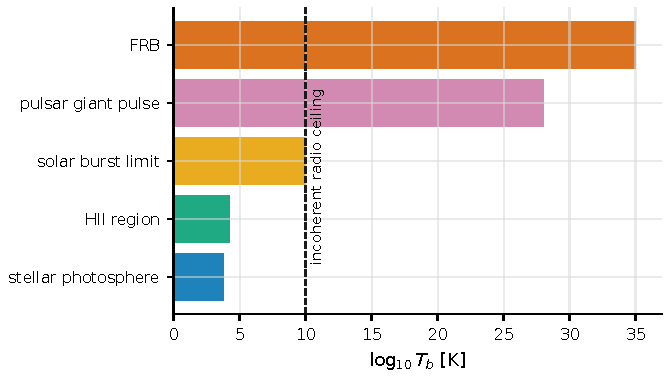
\includegraphics[width=0.82\linewidth]{figures/generated/chapter_09/ch09_brightness_temperature_scale.pdf}
\caption{亮温作为辐射机制判据。恒星光球和 HII 区处在普通热温度范围；太阳和恒星射电爆发若超过 \(10^{10}~{\rm K}\) 往往需要相干机制；脉冲星巨脉冲和 FRB 的亮温更高，只能由相干发射或强束射几何解释。虚线标出常用的非相干射电上限量级。}
\label{fig:chapter-09-brightness-temperature}
\end{figure}

亮温告诉我们“平均能量密度是否合理”，但不能告诉我们这些能量是由大量独立发射事件叠加出来的，还是由带电粒子协同发射出来的。两种光场可以有相同 \(I_\nu\)，却有不同的到达时间、偏振和跨频联合概率。平均谱之外，光子统计从一阶和二阶相干函数进入。若 \(E^{(+)}(t)\) 是正频电场算符，归一化一阶相干函数描述相位和频谱相干，
\begin{equation}
  g^{(1)}(\tau)=
  \frac{\langle E^{(-)}(t)E^{(+)}(t+\tau)\rangle}
       {\langle E^{(-)}(t)E^{(+)}(t)\rangle},
  \label{eq:ch09-g1}
\end{equation}
\begin{formulaexplain}
\(g^{(1)}(\tau)\) 是归一化一阶相干函数；\(E^{(+)}\) 和 \(E^{(-)}\) 是正、负频电场算符。它衡量场相位在时间延迟 \(\tau\) 后还保留多少记忆。
\end{formulaexplain}
而二阶相干函数描述强度涨落和光子到达时间相关，
\begin{equation}
  g^{(2)}(\tau)=
  \frac{\langle I(t)I(t+\tau)\rangle}{\langle I(t)\rangle^2}.
  \label{eq:ch09-g2}
\end{equation}
\begin{formulaexplain}
\(g^{(2)}(\tau)\) 是归一化强度相关；\(I(t)\) 是瞬时强度。它比较一个时刻的光子到达是否会提高另一个时刻的到达概率，是区分聚束、Poisson 和反聚束统计的核心量。
\end{formulaexplain}
式 \eqref{eq:ch09-g1} 问的是场本身隔多久还保留相位记忆，式 \eqref{eq:ch09-g2} 问的是一次光子到达是否会提高另一时刻光子到达的概率。热混沌光在单一时空偏振模式中有 \(g^{(2)}(0)=2\)，相干态有 \(g^{(2)}(0)=1\)。真实天文观测通常同时平均许多时间、频率、空间和偏振模式，热光聚束峰会被稀释为
\begin{equation}
  g^{(2)}_{\rm meas}(0)-1\simeq \frac{1}{M_{\rm eff}},
  \qquad
  M_{\rm eff}\simeq M_{\rm sp}M_{\rm pol}
  \left(1+\frac{\Delta t}{\tau_c}\right).
  \label{eq:ch09-mode-dilution}
\end{equation}
\begin{formulaexplain}
\(M_{\rm eff}\) 是有效混合模式数；\(M_{\rm sp}\)、\(M_{\rm pol}\) 分别是空间和偏振模式数，\(\Delta t/\tau_c\) 描述时间 bin 对相干时间的平均。模式越多，热光聚束对比度越低。
\end{formulaexplain}
\(M_{\rm sp}\) 是被混合的空间模式数，\(M_{\rm pol}\) 是偏振模式数，\(\Delta t\) 是电子或软件时间 bin，\(\tau_c\sim1/\Delta\nu\) 是由光谱带宽决定的相干时间。若 \(\Delta\nu=1~{\rm nm}\) 且 \(\lambda=500~{\rm nm}\)，\(\tau_c\sim0.8~{\rm ps}\)；若电子时间分辨率是 \(100~{\rm ps}\)，单模热光的聚束峰也会被压低两个数量级以上。窄带滤波、偏振选择和空间模式控制提高可见对比度，但会减少光子率。

\begin{figure}[tbp]
\centering
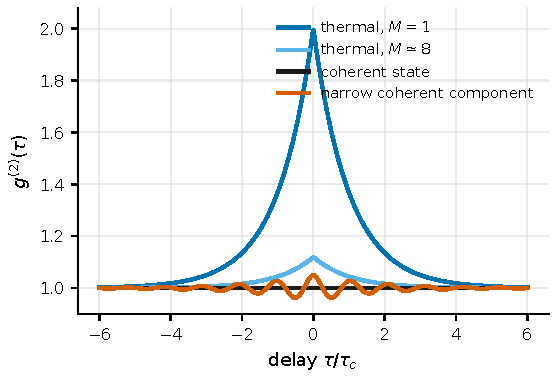
\includegraphics[width=0.82\linewidth]{figures/generated/chapter_09/ch09_radiation_g2_diagnostics.pdf}
\caption{不同光场的 \(g^{(2)}(\tau)\)。单模热光在零延迟处给出高度为 2 的聚束峰；多模平均把峰值压低；理想相干态接近 1；窄相干谱线或受激成分可以在接近 Poisson 的背景上留下小幅振荡或窄峰。横轴按相干时间 \(\tau_c\) 归一化。}
\label{fig:chapter-09-g2-diagnostics}
\end{figure}

\begin{figure}[tbp]
\centering
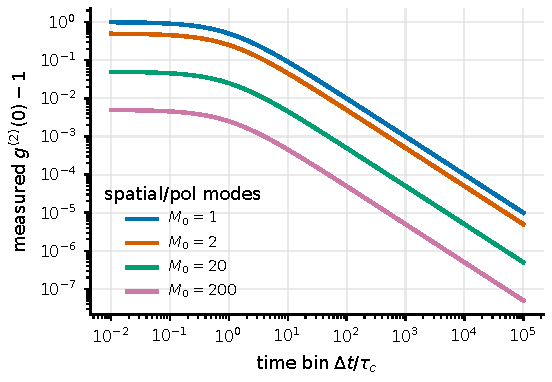
\includegraphics[width=0.82\linewidth]{figures/generated/chapter_09/ch09_thermal_mode_dilution.pdf}
\caption{热光聚束对比度随有效模式数下降。横轴是时间 bin 与相干时间的比值，曲线中的 \(M_0\) 代表进入同一个相关估计器的空间和偏振模式数。即使源本身是热光，宽时间 bin、多偏振混合或多空间模式混合都会让 \(g^{(2)}(0)-1\) 接近零。}
\label{fig:chapter-09-mode-dilution}
\end{figure}

\section{热过程怎样产生近似混沌光}

局部热平衡中的黑体光场由平均占有数
\begin{equation}
  \bar{n}_\nu=
  \frac{1}{\exp(h\nu/k_BT)-1}
  \label{eq:ch09-planck-occupation}
\end{equation}
\begin{formulaexplain}
\(\bar n_\nu\) 是频率 \(\nu\) 模式的平均光子占有数；\(h\nu\) 是单光子能量，\(T\) 是温度。Planck 分布给出热态每个模式中平均有多少光子。
\end{formulaexplain}
决定。这里 \(h\nu\) 是单光子能量，\(T\) 是物质温度。光球、尘埃和 CMB 接近这种热态；恒星光球的可见光 \(h\nu/k_BT\) 不一定处在 Rayleigh--Jeans 极限，因此颜色温度、有效温度和亮温不能混用。热光的相位由许多独立发射体随机叠加，电场近似复高斯过程；在这个条件下 Siegert 关系给出 \(g^{(2)}(\tau)=1+|g^{(1)}(\tau)|^2/M_{\rm eff}\)。

自由自由辐射不是黑体谱本身，而是许多电子在离子库仑场中被加速时发出的连续谱。关键物理图像仍然是“许多独立事件相加”：单次碰撞的相位不可预测，窄带内的复电场会趋向高斯随机过程。稀薄电离气体中，发射系数的数量级可写成
\begin{equation}
  j_\nu^{\rm ff}\propto
  n_e n_i T_e^{-1/2}
  \exp\!\left(-\frac{h\nu}{k_BT_e}\right)
  g_{\rm ff}(\nu,T_e),
  \label{eq:ch09-free-free}
\end{equation}
\begin{formulaexplain}
\(j_\nu^{\rm ff}\) 是自由自由发射系数；\(n_e,n_i\) 是电子和离子密度，\(T_e\) 是电子温度，\(g_{\rm ff}\) 是 Gaunt 因子。它描述许多独立库仑碰撞贡献的连续谱强度。
\end{formulaexplain}
其中 \(n_e\) 和 \(n_i\) 是电子和离子数密度，单位 \({\rm cm^{-3}}\) 或 \({\rm m^{-3}}\)；\(T_e\) 是电子温度；\(g_{\rm ff}\) 是 Gaunt 因子，通常为 1 到数十量级。HII 区的 \(T_e\sim10^4~{\rm K}\)，星风和吸积流可以更高。许多独立碰撞事件叠加后，光场在窄带内仍接近混沌热光；但若观测时间远大于 \(\tau_c\)，可见聚束会被式 \eqref{eq:ch09-mode-dilution} 稀释。

吸收和发射要放在辐射转移方程里：
\begin{equation}
  \frac{{\rm d}I_\nu}{{\rm d}s}=j_\nu-\alpha_\nu I_\nu,
  \qquad
  S_\nu=\frac{j_\nu}{\alpha_\nu}.
  \label{eq:ch09-radiative-transfer}
\end{equation}
\begin{formulaexplain}
\({\rm d}I_\nu/{\rm d}s\) 是视线方向上的强度变化；\(j_\nu\) 加入辐射，\(\alpha_\nu I_\nu\) 吸收辐射，\(S_\nu\) 是源函数。辐射转移把发射机制和光深效应连在一起。
\end{formulaexplain}
\(s\) 是沿视线距离，\(j_\nu\) 是发射系数，\(\alpha_\nu\) 是吸收系数，\(S_\nu\) 是源函数。若换成亮温并用光深 \({\rm d}\tau_\nu=\alpha_\nu{\rm d}s\)，均匀 slab 给出
\begin{equation}
  T_b=T_{\rm eff}\left(1-e^{-\tau_\nu}\right)
      +T_{\rm bg}e^{-\tau_\nu}.
  \label{eq:ch09-tb-transfer}
\end{equation}
\begin{formulaexplain}
\(T_b\) 是出射亮温；\(T_{\rm eff}\) 是源函数对应温度，\(T_{\rm bg}\) 是背景亮温，\(\tau_\nu\) 是光深。薄源只贡献小增量，厚源趋向自身源函数。
\end{formulaexplain}
\(T_{\rm eff}\) 是对应源函数的等效温度，\(T_{\rm bg}\) 是背景亮温。光深很小时 \(T_b\simeq T_{\rm eff}\tau_\nu+T_{\rm bg}\)，光深很大时 \(T_b\to T_{\rm eff}\)。这条式子常用于判断一个源是热化、半透明还是非热发射占优 \citep{1979rpa..book.....R,2011piim.book.....D,1985ARA&A..23..169D}。

\section{非热粒子怎样改变谱和偏振}

同步辐射来自相对论电子在磁场中的螺旋运动。单个电子的特征频率为
\begin{equation}
  \nu_c=\frac{3eB\sin\alpha}{4\pi m_ec}\gamma^2 ,
  \label{eq:ch09-synch-critical}
\end{equation}
\begin{formulaexplain}
\(\nu_c\) 是同步辐射特征频率；\(B\) 是磁场，\(\alpha\) 是 pitch angle，\(\gamma\) 是电子 Lorentz 因子。频率随 \(B\) 和 \(\gamma^2\) 增长，所以高能电子可把辐射推到高频。
\end{formulaexplain}
其中 \(e\) 是元电荷，\(B\) 是磁场强度，\(\alpha\) 是 pitch angle，\(m_e\) 是电子质量，\(\gamma\) 是 Lorentz 因子。若 \(B=1~{\rm G}\)、\(\gamma=10^3\)、\(\sin\alpha=1\)，则 \(\nu_c\simeq4.2\times10^{12}~{\rm Hz}\)，在远红外。若 \(B=10^{-5}~{\rm G}\) 的星系际或喷流尺度磁场中，同样电子主要辐射射电。单电子功率的能谱很宽，真实源的发射系数来自
\begin{equation}
  j_\nu^{\rm syn}=\int P_\nu(E,B,\alpha)\,N(E)\,{\rm d}E .
  \label{eq:ch09-synch-emissivity}
\end{equation}
\begin{formulaexplain}
\(j_\nu^{\rm syn}\) 是同步辐射发射系数；\(P_\nu\) 是单电子功率谱，\(N(E)\) 是电子能量分布。积分表示观测谱是所有能量电子贡献的叠加。
\end{formulaexplain}
\Needspace{12\baselineskip}
若电子能谱 \(N(E)\propto E^{-p}\)，光薄同步辐射给出 \(I_\nu\propto\nu^{-\alpha_{\rm syn}}\)，其中 \(\alpha_{\rm syn}=(p-1)/2\)。最大线偏振度在均匀磁场中约为
\begin{equation}
  \Pi_{\rm syn}=\frac{p+1}{p+7/3}.
  \label{eq:ch09-synch-polarization}
\end{equation}
\begin{formulaexplain}
\(\Pi_{\rm syn}\) 是光薄同步辐射的最大线偏振度；\(p\) 是电子能谱指数。它给出均匀磁场和幂律电子分布下偏振能达到的理论上限。
\end{formulaexplain}
例如 \(p=2.4\) 时 \(\Pi_{\rm syn}\simeq72\%\)。实际喷流、超新星遗迹和脉冲星风云的偏振往往较低，因为磁场方向、法拉第旋转、束内平均和多发射区叠加会抵消偏振。由大量独立电子和湍动单元叠加时，电场也可近似高斯混沌场；与热光不同的是，平均谱和偏振由非热粒子分布和磁场几何决定 \citep{1965ARA&A...3..297G,1970RvMP...42..237B,1978bllo.conf..328B,2012ApJ...752..157Z}。

逆康普顿散射把低能光子提升到高能。Thomson 极限中，散射后光子能量的数量级为
\begin{equation}
  h\nu_{\rm IC}\sim \gamma^2 h\nu_{\rm seed}.
  \label{eq:ch09-ic-energy}
\end{equation}
\begin{formulaexplain}
\(h\nu_{\rm seed}\) 是种子光子能量，\(h\nu_{\rm IC}\) 是散射后能量，\(\gamma\) 是电子 Lorentz 因子。逆康普顿散射在 Thomson 极限中把光子能量提升约 \(\gamma^2\) 倍。
\end{formulaexplain}
热电子云中的多次散射常用 Compton \(y\) 参数判断：
\begin{equation}
  y\simeq
  4\frac{k_BT_e}{m_ec^2}\max(\tau_T,\tau_T^2),
  \label{eq:ch09-compton-y}
\end{equation}
\begin{formulaexplain}
\(y\) 是 Comptonization 强度参数；前因子是单次散射的相对能量增益，\(\max(\tau_T,\tau_T^2)\) 估计平均散射次数。它判断谱会被电子云改写到什么程度。
\end{formulaexplain}
其中 \(T_e\) 是电子温度，\(\tau_T\) 是 Thomson 光深。\(y\ll1\) 时谱只被轻微改变；\(y\sim1\) 时会形成明显的 Comptonized continuum；\(y\gg1\) 时趋向饱和 Comptonization。X 射线双星、AGN corona 和 GRB photosphere 模型中，平均谱可以由同步、热光子和逆康普顿多分量混合形成，单靠谱指数很难唯一判定机制 \citep{1980A&A....86..121S,1999MNRAS.309..496G,2013ApJ...765..103L}。

\begin{figure}[tbp]
\centering
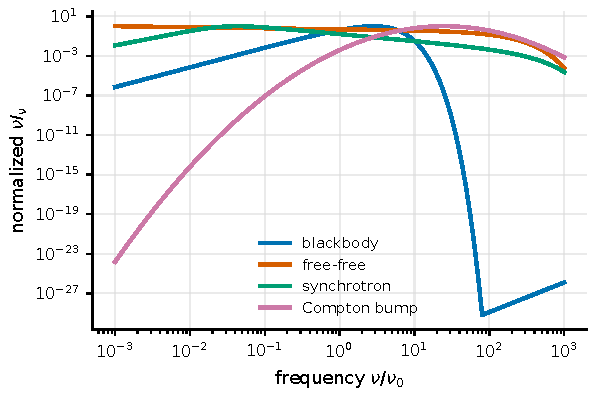
\includegraphics[width=0.84\linewidth]{figures/generated/chapter_09/ch09_spectral_mechanisms.pdf}
\caption{常见连续辐射机制的归一化谱形示意。黑体有热峰和 Rayleigh--Jeans 低频端；自由自由辐射在射电可近似平坦并在高频指数衰减；同步辐射由非热电子能谱给出幂律和高低频截断；逆康普顿分量常表现为高能 bump。真实源需要把这些分量放进辐射转移和几何模型中联合拟合。}
\label{fig:chapter-09-spectral-mechanisms}
\end{figure}

\section{相干机制怎样突破亮温上限}

Maser 从负吸收开始。若某条谱线存在粒子数反转，吸收系数可为负，写成 \(\alpha_\nu<0\)。沿路径的强度近似满足
\begin{equation}
  I_\nu(L)\simeq I_\nu(0)\exp(|\tau_m|),
  \qquad
  \tau_m=\int_0^L\alpha_\nu\,{\rm d}s<0 .
  \label{eq:ch09-maser-gain}
\end{equation}
\begin{formulaexplain}
\(I_\nu(0)\) 和 \(I_\nu(L)\) 是路径前后的强度；\(\tau_m<0\) 是负吸收光深。Maser 的无饱和增益随 \(|\tau_m|\) 指数增长，这是高亮温窄线的来源。
\end{formulaexplain}
无饱和时，增益对光深指数敏感；饱和后，受激辐射耗尽反转，线宽、偏振和强度随泵浦与几何改变。水 maser、OH maser 和 SiO maser 的亮温可极高，但它们的相干性通常由许多速度相干路径、湍动团块和偏振传播效应共同决定，不能简单等同于实验室单模激光。Goldreich、Keeley、Kwan 和 Elitzur 的工作给出了源尺寸、饱和、线宽与偏振的基本约束 \citep{1972ApJ...174..517G,1973ApJ...179..111G,1974ApJ...190...27G,1982RvMP...54.1225E,1992ARA&A..30...75E}。

电子回旋 maser 是强磁化低密度等离子体中的相干射电机制。它要求电子分布偏离平衡，例如 loss-cone 分布，并且磁场频率与等离子体频率的关系允许电磁波逃逸。回旋频率为
\begin{equation}
  \nu_B=\frac{eB}{2\pi m_ec}
       \simeq 2.8~{\rm MHz}\left(\frac{B}{1~{\rm G}}\right).
  \label{eq:ch09-cyclotron-frequency}
\end{equation}
\begin{formulaexplain}
\(\nu_B\) 是电子回旋频率；\(e\) 是电荷，\(B\) 是磁场，\(m_e\) 是电子质量。观测到的 maser 频率可反推发射区磁场量级。
\end{formulaexplain}
若在 GHz 频率看到基频或低次谐波 electron-cyclotron maser，磁场量级是几百 G 到几 kG。太阳、行星、褐矮星和低质量恒星的高圆偏振射电爆发都可落在这个框架中 \citep{1982ApJ...259..844M,2006A&ARv..13..229T,2008ApJ...684..644H,1985ARA&A..23..169D}。

曲率辐射展示了另一条通往相干性的路。它不一定依赖能级反转，而是让许多电荷在相位上协同运动。相对论电荷沿弯曲磁力线运动时，单个电荷的特征频率和功率为
\begin{equation}
  \nu_{\rm curv}=\frac{3c}{4\pi\rho}\gamma^3,
  \qquad
  P_{\rm curv}=\frac{2e^2c}{3\rho^2}\gamma^4 ,
  \label{eq:ch09-curvature}
\end{equation}
\begin{formulaexplain}
\(\nu_{\rm curv}\) 是曲率辐射特征频率，\(P_{\rm curv}\) 是单粒子功率；\(\rho\) 是磁力线曲率半径，\(\gamma\) 是 Lorentz 因子。相干曲率辐射还需要许多电荷相位同步。
\end{formulaexplain}
其中 \(\rho\) 是磁力线曲率半径。若 \(\rho=10^7~{\rm cm}\) 且 \(\gamma=300\)，\(\nu_{\rm curv}\sim2\times10^9~{\rm Hz}\)。单个粒子的曲率辐射仍然太弱；相干曲率辐射要求许多电荷在小于波长的纵向尺度上成团，电场振幅相加，功率可近似随粒子数平方增长。这个思路长期用于脉冲星相干射电，也被用于 FRB 模型 \citep{1977ApJ...212..800C,2018MNRAS.477.2470L}。

FRB 的观测把这些机制推到极端。Lorimer burst 给出了毫秒时间尺度、冷等离子体色散和 \(T_b\sim10^{34}~{\rm K}\) 量级的第一组证据；重复源和 CHIME 样本显示，重复、偏振、漂移、微结构和宿主环境都会进入模型；SGR 1935+2154 的 2020 年事件把银河系 magnetar 和 FRB-like radio burst 直接连在一起 \citep{2007Sci...318..777L,2019A&ARv..27....4P,2022A&ARv..30....2P,2020Natur.587...54C,2020Natur.587...59B}。许多模型可分成两类：靠 population inversion 或激波产生的 maser 类机制，以及靠电荷团块或电流片产生的 antenna/curvature 类机制。微秒以下结构、强偏振、频率漂移和多波段非探测共同限制发射半径、Lorentz 因子、等离子体密度和辐射效率。

光学自然激光是另一种受激辐射案例。Eta Carinae 的 Weigelt blobs 中，Fe II 和 O I 线可在特定泵浦和光深条件下出现激光或激光样放大；这类线的宽度、空间位置、偏振和光子相关可检验反转与反馈几何 \citep{2004A&A...428..497J,2005NewA...10..361J,2008AIPC..984..216D}。受激辐射可以出现在射电 maser 之外的环境中；只要泵浦、能级结构和逃逸路径合适，光学谱线也可能带有非普通热光的统计特征。

\section{怎样把机制判断变成联合诊断}

实际分类时，平均谱只给第一层线索。区分热源、同步源、maser 和相干爆发，需要把谱、偏振、相关函数、时间尺度和角尺度放在同一个观测向量里：
\begin{equation}
  {\bf d}=
  \left\{
  I_\nu(t),\,
  Q_\nu(t),U_\nu(t),V_\nu(t),\,
  g^{(2)}_{ab}(\tau;\nu_i,\nu_j),\,
  \Delta t_{\rm var},\,
  \Omega_{\rm s}
  \right\}.
  \label{eq:ch09-diagnostic-vector}
\end{equation}
\begin{formulaexplain}
\({\bf d}\) 是机制诊断观测向量；它同时收集强度、Stokes 偏振、二阶相关、变异时间和角尺度。辐射机制判断需要这些量联合约束，而不是只看平均谱。
\end{formulaexplain}
\(Q,U,V\) 是 Stokes 参数，\(a,b\) 标记望远镜、偏振或频率通道，\(\Delta t_{\rm var}\) 是变异时间尺度，\(\Omega_{\rm s}\) 是角尺度约束。热源通常有低偏振、有限 \(T_b\) 和热聚束；光薄同步辐射可有高线偏振和幂律谱；maser 以窄线、高亮温和强偏振为特征；FRB 以极高亮温、毫秒到微秒结构、色散和强偏振为典型特征；散射和等离子体传播会改变时间结构和频谱，却不应被误认为源本身的发射统计。

\begin{figure}[tbp]
\centering
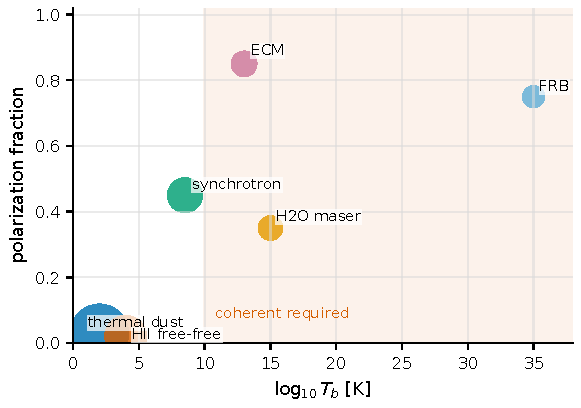
\includegraphics[width=0.86\linewidth]{figures/generated/chapter_09/ch09_diagnostic_plane.pdf}
\caption{辐射机制的联合诊断平面。横轴是亮温，纵轴是偏振分数，点大小表示可见二阶相干对比度的量级。热尘埃和 HII 区位于低亮温低偏振区域；同步辐射偏振较高但亮温通常低于相干爆发；electron-cyclotron maser、分子 maser 和 FRB 进入高亮温区域，需要解释相干发射、泵浦或电荷成团。}
\label{fig:chapter-09-diagnostic-plane}
\end{figure}

在数据分析中，\(g^{(2)}\) 的异常峰值要先和仪器、传播效应和混合源逐项比对。死时间、afterpulsing、时间戳量化和触发选择会改写到达时间相关；等离子体闪烁、散射尾、引力微透镜和频率依赖吸收会产生跨频相关；热背景叠加窄 maser 线，或同步连续谱叠加相干脉冲，也会让平均谱看起来平滑而光子统计不再单一。第 \ref{chap:06} 章和第 \ref{chap:07} 章的事件表、时间移位背景和协方差估计提供了这类排查所需的分析层。


\chapter{恒星作为量子光源}
\label{chap:10}

\begin{chapteropening}
恒星很适合作为第一批量子天文学目标。光球连续谱近似热光，亮星有足够光子率，角直径在毫角秒量级；强度干涉可以直接测 \(|V|^2\)，不要求望远镜之间保持光学相位。但恒星表面并非完美圆盘。边缘昏暗、快速自转、星斑、双星、脉动和星风都会把表面亮度分布写进可见度曲线。前面建立的相干函数、事件表和 Fisher 信息，在恒星问题中对应半径、有效温度、旋转和距离标尺 \citep{1956Natur.177...27B,1967MNRAS.137..375H,1967MNRAS.137..393H,1974MNRAS.167..121H,1974iiia.book.....H,2020NatAs...4.1164A,2024MNRAS.529.4387A}。
\end{chapteropening}

\section{为什么恒星是最稳的标定场}

恒星光球在局部热平衡下发出近似热辐射。单个相干模式的热光有 \(g^{(2)}(0)=2\)，但真实恒星观测混合了大量空间、偏振、频率和时间模式，实际可见的 \(g^{(2)}(0)-1\) 很小。Vega photon-counting 强度干涉实验在零基线测得 \(\langle g^{(2)}\rangle=1.0034\pm0.0008\)，在约 \(2~{\rm km}\) 基线上没有显著相关，结果与 Vega 约 \(3.3~{\rm mas}\) 的角直径相容 \citep{2021MNRAS.506.1585Z}。这是第 \ref{chap:09} 章模式数稀释在恒星上的实际版本。

强度干涉测量的是两台望远镜光强涨落的相关。对热光，校准后的零延迟相关与复可见度满足
\begin{equation}
  g^{(2)}_{ij}(0)-1 = |\gamma_{ij}|^2 \simeq |V(u_{ij},v_{ij})|^2 .
  \label{eq:ch10-g2-visibility}
\end{equation}
\begin{formulaexplain}
\(g^{(2)}_{ij}(0)\) 是望远镜 \(i,j\) 的零延迟强度相关；\(\gamma_{ij}\) 是复相干度，\(V\) 是归一化可见度。热光强度干涉把相关超额变成天空亮度 Fourier 模平方。
\end{formulaexplain}
\(\gamma_{ij}\) 是两台望远镜之间的复相干度，\((u,v)={\bf B}_\perp/\lambda\) 是投影基线除以波长，单位是波长数。观测中左边来自延迟直方图、时间移位背景扣除和归一化相关；右边是天空亮度分布的 Fourier 模平方。相位丢失意味着 \(|V|^2\) 对镜像和整体平移不敏感，但角直径、轴比、双星间距和某些对称结构仍可精确测量。

基线和角尺度由同一个比例给出：
\begin{equation}
  B\sim\frac{\lambda}{\theta}
  \simeq 103~{\rm m}
  \left(\frac{\lambda}{500~{\rm nm}}\right)
  \left(\frac{\theta}{1~{\rm mas}}\right)^{-1}.
  \label{eq:ch10-baseline-scale}
\end{equation}
\begin{formulaexplain}
\(B\) 是基线长度，\(\lambda\) 是波长，\(\theta\) 是目标角尺度。这个比例说明可见光百米基线对应毫角秒恒星，公里基线才进入更小表面结构。
\end{formulaexplain}
一个 \(1~{\rm mas}\) 的恒星在可见光需要百米基线开始明显分辨；\(0.1~{\rm mas}\) 的表面结构需要公里量级基线。Narrabri 强度干涉仪用 \(10\)--\(188~{\rm m}\) 基线和两个 \(6.7~{\rm m}\) 反射面测量了 32 颗亮星角直径；现代 VERITAS、MAGIC 和未来 CTA 类型阵列用 \(>10~{\rm m}\) 级 Cherenkov 望远镜、大面积收光和数字相关器重新打开了这个参数空间 \citep{1974MNRAS.167..121H,2012NewAR..56..143D,2020NatAs...4.1164A,2024MNRAS.529.4387A}。

强度干涉的信噪比标度已在式 \eqref{eq:ch05-snr} 给出。放到恒星样本上，它的主要含义很直接：光子率越高、电子带宽越大、积分越久，\(|V|^2\) 的误差越小；背景、死时间、有限时间分辨率和系统协方差则决定这种统计增益会在哪里停止。因此第一批样本自然偏向亮、热、蓝、角直径在百米级基线可分辨的恒星 \citep{2013MNRAS.430.3187R,2020NatAs...4.1164A}。

\section{怎样从平方可见度读出角直径和温度}

从数据到半径的第一步，是把恒星暂时当成一个只有角直径的圆盘。最基础的恒星模型仍是第 \ref{chap:05} 章的均匀圆盘，使用式 \eqref{eq:ch05-uniform-disk}。这里 \(B\) 是投影基线，\(\lambda\) 是有效波长，\(\theta\) 用弧度；若 \(\theta\) 以 mas 给出，要乘以 \(4.848\times10^{-9}\) 转成弧度。强度干涉拟合的是 \(|V_{\rm UD}|^2\)，复相位已经被平方模取代。第一零点附近对角直径最敏感，但 \(|V|^2\) 太低时系统误差和背景会变得重要，所以实际观测要覆盖短、中、长基线。短基线固定总通量和相关归一化，中等基线给出直径斜率，长基线检查模型是否需要边缘昏暗、扁率或伴星。

\begin{figure}[tbp]
\centering
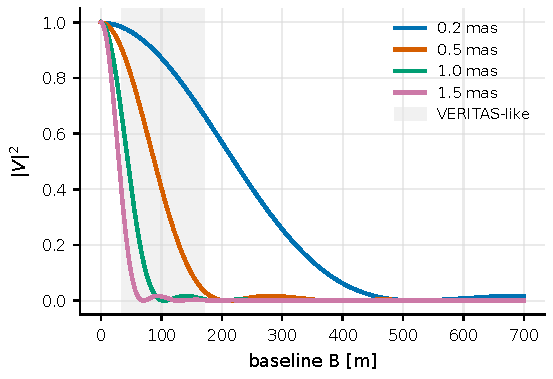
\includegraphics[width=0.82\linewidth]{figures/generated/chapter_10/ch10_stellar_diameter_visibility.pdf}
\caption{均匀圆盘恒星的 \(|V|^2\) 随基线变化。波长取 \(416~{\rm nm}\)，接近 VERITAS SII 的观测波长。角直径越大，可见度下降越快；灰色区域标出 \(35\)--\(170~{\rm m}\) 的 VERITAS 量级投影基线范围，适合测量约 \(0.5\)--\(1.5~{\rm mas}\) 的亮星。}
\label{fig:chapter-10-diameter-visibility}
\end{figure}

角直径和总辐射流量给出有效温度。若 \(F_{\rm bol}\) 是地球处测得的 bolometric flux，单位 \({\rm erg\,s^{-1}\,cm^{-2}}\)，则
\begin{equation}
  F_{\rm bol}=\frac{\theta_{\rm LD}^2}{4}
  \sigma_{\rm SB}T_{\rm eff}^4,
  \qquad
  T_{\rm eff}=
  \left(\frac{4F_{\rm bol}}{\sigma_{\rm SB}\theta_{\rm LD}^2}\right)^{1/4}.
  \label{eq:ch10-teff}
\end{equation}
\begin{formulaexplain}
\(F_{\rm bol}\) 是地球处总辐射流量，\(\theta_{\rm LD}\) 是边缘昏暗角直径，\(\sigma_{\rm SB}\) 是 Stefan--Boltzmann 常数。角直径和总流量共同给出有效温度。
\end{formulaexplain}
\(\theta_{\rm LD}\) 是边缘昏暗角直径，\(\sigma_{\rm SB}\) 是 Stefan--Boltzmann 常数。误差传播为
\begin{equation}
  \left(\frac{\sigma_T}{T_{\rm eff}}\right)^2
  \simeq
  \frac{1}{16}\left(\frac{\sigma_F}{F_{\rm bol}}\right)^2
  +\frac{1}{4}\left(\frac{\sigma_\theta}{\theta_{\rm LD}}\right)^2 .
  \label{eq:ch10-teff-error}
\end{equation}
\begin{formulaexplain}
\(\sigma_T,\sigma_F,\sigma_\theta\) 分别是温度、总流量和角直径误差。因为 \(T_{\rm eff}\propto F_{\rm bol}^{1/4}\theta_{\rm LD}^{-1/2}\)，同等百分比下角直径误差更重要。
\end{formulaexplain}
角直径误差进入系数是 \(1/2\)，常常主导 \(T_{\rm eff}\)。VERITAS 对 \(\beta\) UMa 的 SII 观测得到 \(\theta_{\rm LD}=1.07\pm0.04{\rm(stat)}\pm0.05{\rm(sys)}~{\rm mas}\)，由此给出 \(T_{\rm eff}\simeq9700\pm200\pm200~{\rm K}\)，并可进一步约束 Ursa Major moving group 的年龄 \citep{2024ApJ...966...28A}。

\begin{figure}[tbp]
\centering
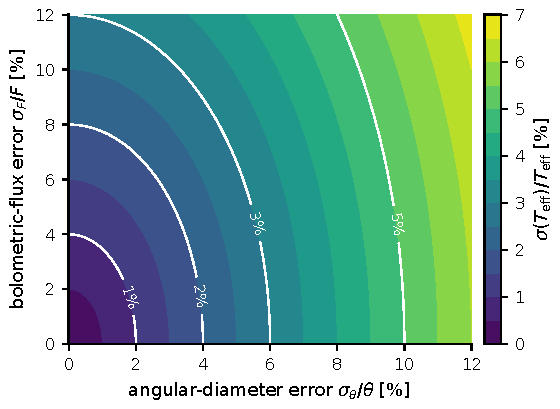
\includegraphics[width=0.78\linewidth]{figures/generated/chapter_10/ch10_teff_error_budget.pdf}
\caption{由 \(F_{\rm bol}\) 和 \(\theta_{\rm LD}\) 推导 \(T_{\rm eff}\) 的误差传播。横轴是角直径相对误差，纵轴是总流量相对误差，颜色给出有效温度相对误差。由于 \(T_{\rm eff}\propto F_{\rm bol}^{1/4}\theta^{-1/2}\)，角直径误差通常比同等百分比的流量误差更重要。}
\label{fig:chapter-10-teff-error}
\end{figure}

\Needspace{13\baselineskip}
若距离 \(d\) 已知，半径和光度为
\begin{equation}
  R=\frac{1}{2}\theta_{\rm LD}d,\qquad
  L=4\pi R^2\sigma_{\rm SB}T_{\rm eff}^4 .
  \label{eq:ch10-radius-luminosity}
\end{equation}
\begin{formulaexplain}
\(R\) 是恒星半径，\(d\) 是距离，\(L\) 是光度。角直径给出天空上的大小，距离把它变成物理半径，再由 Stefan--Boltzmann 定律得到光度。
\end{formulaexplain}
Gaia 视差、干涉角直径和 \(F_{\rm bol}\) 联合后，恒星会落到 HR 图上一个带协方差的区域。这个区域与演化轨道比较给出质量、年龄和混合长度、超调、旋转等模型约束。红外流量法、Mark III/CHARA 等振幅干涉角直径和 SII 角直径在这一层面是互补的标尺 \citep{1977MNRAS.180..177B,1991AJ....101.2207M,1994A&A...282..899B,2003AJ....126.2502M,2005ApJ...626..446R}。

\section{边缘昏暗为什么不是小修正}

真实恒星边缘更暗，因为视线穿过的温度层不同。最简单的线性边缘昏暗模型为
\begin{equation}
  I(\mu)=I(1)\,[1-u_\lambda(1-\mu)],
  \qquad
  \mu=\sqrt{1-r^2}.
  \label{eq:ch10-linear-ld}
\end{equation}
\begin{formulaexplain}
\(I(\mu)\) 是不同视角处的表面亮度；\(\mu\) 是法线与视线夹角余弦，\(r\) 是归一化投影半径，\(u_\lambda\) 是边缘昏暗系数。它把恒星边缘变暗写成一个简化剖面。
\end{formulaexplain}
\(r\) 是投影圆盘半径除以恒星半径，\(\mu\) 是表面法线与视线夹角的余弦，\(u_\lambda\) 是波长相关的边缘昏暗系数。热星在蓝光、冷巨星在分子带、Mira 变量在不同相位都会有不同的 \(I(\mu)\)。现代分析通常从大气模型或 limb-darkening toolkit 生成合成强度分布，再计算可见度；线性 \(u_\lambda\) 更适合做数量级估算 \citep{1974MNRAS.167..475H,1992A&A...259..227D,1997A&A...327..199H,2015MNRAS.453.3821P}。

轴对称亮度分布的可见度是径向 Hankel 变换：
\begin{equation}
  V(x)=
  \frac{\int_0^1 I(r)J_0(xr)\,r\,{\rm d}r}
       {\int_0^1 I(r)\,r\,{\rm d}r}.
  \label{eq:ch10-hankel}
\end{equation}
\begin{formulaexplain}
\(V(x)\) 是轴对称亮度分布的可见度；\(J_0\) 是零阶 Bessel 函数，\(x\) 是基线、波长和角半径组成的无量纲频率。Hankel 变换把径向亮度剖面映射到 \(|V|^2\) 曲线。
\end{formulaexplain}
这里 \(J_0\) 是零阶 Bessel 函数。均匀圆盘是 \(I(r)=\) 常数的特例，回到式 \eqref{eq:ch05-uniform-disk}。边缘昏暗会改变零点位置和旁瓣高度，因此同一组 \(|V|^2\) 数据若用均匀圆盘拟合，会得到 \(\theta_{\rm UD}\)；若用大气模型拟合，会得到更接近物理半径的 \(\theta_{\rm LD}\)。Narrabri 的角直径目录就需要把均匀圆盘直径修正为 limb-darkened 直径 \citep{1974MNRAS.167..121H,1974MNRAS.167..475H}。

\begin{figure}[tbp]
\centering
\includegraphics[width=0.92\linewidth]{figures/generated/chapter_10/ch10_limb_darkening.pdf}
\caption{线性边缘昏暗对表面亮度和可见度的影响。左图显示 \(u_\lambda=0,0.4,0.8\) 时的径向亮度；右图用式 \eqref{eq:ch10-hankel} 数值积分得到 \(|V|^2\)。边缘越暗，圆盘边界越不尖锐，可见度零点和旁瓣相应移动。}
\label{fig:chapter-10-limb-darkening}
\end{figure}

边缘昏暗也是系统误差来源。它改变的不是一个绘图细节，而是“哪个半径正在被测量”。热星的 \(u_\lambda\) 取决于 \(T_{\rm eff}\)、\(\log g\)、金属丰度、微湍流和滤光片；冷巨星和 Mira 的半径还随波长变化，分子层会让“角直径”变成谱带依赖量。若目标用于标定另一个源，校准星的单星性、旋转、伴星、红外过量和光变都要检查。对 SII，标定误差来自星表角直径、相关器增益、时间同步、背景光和 \(|V|^2\) 协方差的共同作用。

\section{自转、双星和表面结构怎样进入可见度}

快速自转会让光球变成扁球，并通过 gravity darkening 改变表面温度。若把投影光球近似为椭圆，基线方向 \(\psi\) 上的有效角直径可写成
\begin{equation}
  \theta_{\rm eff}^2(\psi)=
  \theta_{\rm maj}^2\cos^2\psi+
  \theta_{\rm min}^2\sin^2\psi .
  \label{eq:ch10-ellipse-effective}
\end{equation}
\begin{formulaexplain}
\(\theta_{\rm eff}(\psi)\) 是基线方向 \(\psi\) 上看到的有效角直径；\(\theta_{\rm maj}\)、\(\theta_{\rm min}\) 是投影长短轴。快速自转导致的扁率会让 \(|V|^2\) 随位置角改变。
\end{formulaexplain}
\(\theta_{\rm maj}\) 和 \(\theta_{\rm min}\) 分别是投影长轴和短轴角直径。不同位置角的基线会看到不同的 \(|V|^2\) 下降速度。VERITAS 在 \(416~{\rm nm}\) 对 \(\gamma\) Cassiopeiae 的 SII 观测给出 minor-axis angular diameter \(0.43\pm0.02~{\rm mas}\)，major-to-minor radius ratio \(1.28\pm0.04\)，位置角 \(116^\circ\pm5^\circ\)；快速自转大气模型进一步给出接近 breakup 的旋转速度下限和赤道半径约 \(10.9~R_\odot\) \citep{2025ApJ...995..191A}。

\begin{figure}[tbp]
\centering
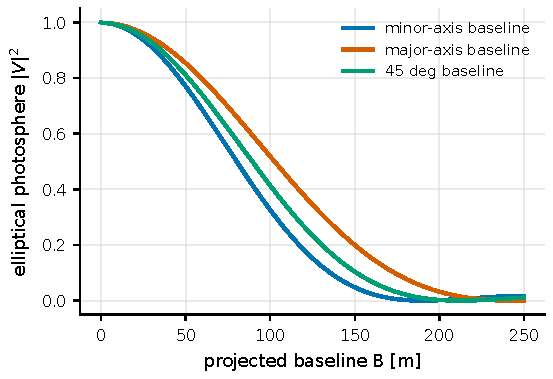
\includegraphics[width=0.82\linewidth]{figures/generated/chapter_10/ch10_rotation_oblateness.pdf}
\caption{快速自转椭圆光球在不同基线方向上的 \(|V|^2\)。参数取 \(\gamma\) Cas 量级的轴比 \(1.28\) 和 \(416~{\rm nm}\) 波长。沿不同位置角投影时，有效角直径不同，因此同一基线长度给出的相关强度也不同；这一几何效应使 SII 能测 photosphere oblateness。}
\label{fig:chapter-10-rotation}
\end{figure}

\Needspace{13\baselineskip}
双星在可见度空间中产生振荡。若两颗星本身未分辨，角分离向量为 \({\boldsymbol d}\)，次星与主星流量比为 \(f\)，则
\begin{equation}
  |V_{\rm bin}|^2=
  \frac{1+f^2+2f\cos(2\pi{\boldsymbol u}\cdot{\boldsymbol d})}
       {(1+f)^2}.
  \label{eq:ch10-binary}
\end{equation}
\begin{formulaexplain}
\(|V_{\rm bin}|^2\) 是未分辨双星的平方可见度；\(f\) 是流量比，\({\boldsymbol u}\) 是空间频率，\({\boldsymbol d}\) 是角分离向量。余弦项让双星在基线空间产生振荡。
\end{formulaexplain}
\({\boldsymbol u}={\boldsymbol B}_\perp/\lambda\)，\({\boldsymbol d}\) 用弧度。振荡周期给出沿基线方向的分离，振幅给出流量比；若每颗星被部分分辨，还要把各自的圆盘可见度乘进去。Narrabri 目录中一些目标后来被识别为双星或多星，现代 SII 多基线阵列可以把双星轨道、角直径和亮度比联合拟合，再与径向速度结合得到质量 \citep{1970MNRAS.148..103H,1974MNRAS.167..121H,2012MNRAS.419..172N}。

\begin{figure}[tbp]
\centering
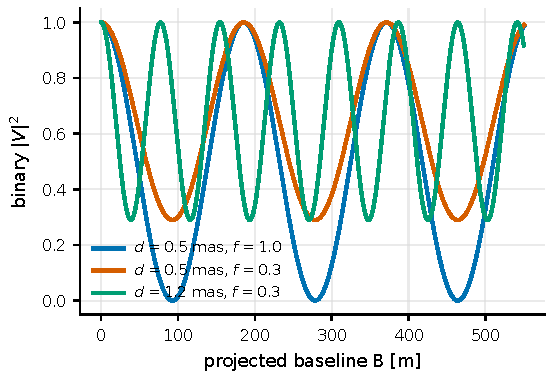
\includegraphics[width=0.82\linewidth]{figures/generated/chapter_10/ch10_binary_visibility.pdf}
\caption{未分辨双星的 \(|V|^2\) 振荡。角分离越大，随基线振荡越快；流量比越接近 1，振荡幅度越大。真实双星还需要加入两颗星的有限角直径、轨道位置角和多波长流量比。}
\label{fig:chapter-10-binary}
\end{figure}

表面结构比双星更难，因为 \(|V|^2\) 缺少相位。星斑、对流单元、非径向脉动和 Be 星盘都会引入非轴对称信号；只用一个圆盘或双星模型可能给出看似漂亮但物理错误的拟合。多基线、多夜晚、多波长和谱线通道可以破除一部分退化。模拟研究显示，Cherenkov 望远镜阵列的基线数量和覆盖范围有机会重建直径、扁率、双星结构和大尺度表面特征，但复杂图像仍需要先验或联合振幅干涉数据 \citep{2012MNRAS.419..172N,2013MNRAS.430.3187R,2012NewAR..56..143D}。

\section{时间变化和谱线通道怎样扩展恒星图像}

造父变星把角直径测量连接到距离标尺。Baade--Wesselink 类方法比较角半径变化和视向速度积分：
\begin{equation}
  \Delta\theta(t)=\frac{2}{d}
  \int p\,[v_r(t)-v_\gamma]\,{\rm d}t .
  \label{eq:ch10-baade-wesselink}
\end{equation}
\begin{formulaexplain}
\(\Delta\theta(t)\) 是角直径变化，\(d\) 是距离，\(v_r-v_\gamma\) 是扣除系统速度后的径向速度，\(p\) 是投影因子。它把脉动速度积分和角半径变化联系起来。
\end{formulaexplain}
\(d\) 是距离，\(v_r\) 是径向速度，\(v_\gamma\) 是系统速度，\(p\) 是把观测径向速度转换为真实脉动速度的投影因子。角直径曲线和速度曲线相位匹配后可求距离。系统误差来自 \(p\) 因子、边缘昏暗、伴星污染、周期变化和大气速度梯度。明亮造父在可见光 SII 中尤其有吸引力，因为它们既亮又有可预测的半径变化 \citep{1997A&A...320..799F,2007A&A...476...73F,2012NewAR..56..143D}。

Be 星和 Wolf--Rayet 星把连续谱和谱线空间结构分开。若窄带滤波器覆盖一条发射线，观测可见度是连续谱和线区的通量加权和：
\begin{equation}
  V_{\rm obs}=
  \frac{F_{\rm cont}V_{\rm cont}+F_{\rm line}V_{\rm line}}
       {F_{\rm cont}+F_{\rm line}} .
  \label{eq:ch10-line-visibility}
\end{equation}
\begin{formulaexplain}
\(V_{\rm obs}\) 是窄带观测到的可见度；连续谱和谱线分量按通量 \(F_{\rm cont},F_{\rm line}\) 加权。若连续谱已标定，就能反推出谱线形成区的空间尺度。
\end{formulaexplain}
若连续谱光球已由邻近谱带标定，就可以反推出谱线形成区的 \(V_{\rm line}\)，进而约束盘半径、倾角或星风几何。对于快速旋转 Be 星，H\(\alpha\) 谱线给盘，蓝光连续谱给光球；\(\gamma\) Cas 的例子表明，SII 可以直接测到光球扁率，而红外或 H\(\alpha\) 干涉则补充盘的几何 \citep{2025ApJ...995..191A}。

自然激光和受激谱线在恒星环境中也可能出现，尤其是 \(\eta\) Carinae 这类强辐射场和密集气体团块共存的系统。对这类目标，普通谱线强度不足以证明受激辐射；需要同时看线宽、空间位置、泵浦通道、偏振和谱线通道的 \(g^{(2)}\)。第 \ref{chap:09} 章讨论的自然激光诊断可转化为具体目标选择 \citep{2004A&A...428..497J,2005NewA...10..361J,2008AIPC..984..216D}。


\chapter{白矮星、中子星和强场物理}
\label{chap:11}

\begin{chapteropening}
白矮星和中子星把量子物理推到天文尺度。白矮星的半径由电子简并压、库仑修正和包层结构决定；中子星的光变由强引力、强磁场和相对论磁层共同投影到事件表上。可测量的仍是到达时间、能量、偏振和相位，只是这些量现在对应 \(10^6\) 到 \(10^{15}\,\mathrm{G}\) 的磁场、毫秒到小时的周期、以及 \(10\,\mathrm{km}\) 到地球半径量级的发光区域。
\end{chapteropening}

\section{白矮星：电子简并压怎样变成可测半径}

白矮星的主标度可由冷费米气体近似来理解。一个质量 \(M\simeq 0.6\,M_\odot\)、半径 \(R\simeq 0.012\,R_\odot\simeq 1.3\,R_\oplus\) 的典型 DA 白矮星，平均密度已经达到 \(10^6\,\mathrm{g\,cm^{-3}}\) 量级，中心密度可到 \(10^6-10^9\,\mathrm{g\,cm^{-3}}\)。在这种密度下，电子热运动只占次要地位；Pauli 不相容原理给电子填满动量空间，费米动量为
\begin{equation}
  p_F=\hbar (3\pi^2 n_e)^{1/3}, \qquad n_e=\frac{\rho}{\mu_e m_p}.
  \label{eq:ch11-01}
\end{equation}
\begin{formulaexplain}
\(p_F\) 是电子费米动量，\(n_e\) 是电子数密度；\(\rho\)、\(\mu_e\)、\(m_p\) 把质量密度换成电子数。它说明白矮星越密，电子被 Pauli 原理推到越高动量。
\end{formulaexplain}
这里 \(n_e\) 是电子数密度，单位 \(\mathrm{cm^{-3}}\)；\(\rho\) 是质量密度；\(m_p\) 是质子质量；\(\mu_e\) 是每个电子对应的重子数，碳氧白矮星通常取 \(\mu_e\simeq2\)。当 \(p_F\ll m_e c\) 时，电子非相对论，压强为
\begin{equation}
  P_{\rm NR}=\frac{(3\pi^2)^{2/3}}{5}\frac{\hbar^2}{m_e}n_e^{5/3};
  \label{eq:ch11-02}
\end{equation}
\begin{formulaexplain}
\(P_{\rm NR}\) 是非相对论电子简并压，随 \(n_e^{5/3}\) 增长。这个很硬的压强标度是普通白矮星能抵抗引力塌缩的主支撑。
\end{formulaexplain}
当 \(p_F\gtrsim m_e c\) 时，相对论效应把指数改成 \(4/3\)，
\begin{equation}
  P_{\rm ER}=\frac{(3\pi^2)^{1/3}}{4}\hbar c\, n_e^{4/3}.
  \label{eq:ch11-03}
\end{equation}
\begin{formulaexplain}
\(P_{\rm ER}\) 是极端相对论电子简并压，密度指数降为 \(4/3\)。支撑变软后，高质量白矮星半径会急剧缩小并接近极限质量。
\end{formulaexplain}
式中 \(P\) 的单位是 \(\mathrm{dyn\,cm^{-2}}\)。非相对论公式中，密度升高会迅速增加支撑压强；相对论公式中，高质量白矮星的支撑变得更软，质量继续增加时半径急剧变小，并走向 Chandrasekhar 极限 \citep{1931ApJ....74...81C,1935MNRAS..95..207C,1961ApJ...134..683H}。

实际写成观测者常用的质量半径近似，可用 Nauenberg 形式
\begin{equation}
  R\simeq 0.0112\,R_\odot
  \left[\left(\frac{M_{\rm Ch}}{M}\right)^{2/3}
  -\left(\frac{M}{M_{\rm Ch}}\right)^{2/3}\right]^{1/2},
  \qquad M_{\rm Ch}\simeq 5.83\,\mu_e^{-2}M_\odot .
  \label{eq:ch11-04}
\end{equation}
\begin{formulaexplain}
\(R\) 是白矮星半径，\(M\) 是质量，\(M_{\rm Ch}\) 是 Chandrasekhar 质量。质量越接近 \(M_{\rm Ch}\)，方括号越小，理想冷白矮星半径越小。
\end{formulaexplain}
这里 \(M_{\rm Ch}\) 是理想冷白矮星极限质量；对 \(\mu_e=2\)，\(M_{\rm Ch}\simeq1.46\,M_\odot\)。这个公式假设零温、非旋转、没有强磁场形变，适合用来估算 \(0.2-1.35\,M_\odot\) 白矮星的主标度。真实半径还受核心组成、氢氦包层厚度、有限温度和磁场影响，高精度工作需要演化模型或双星约束 \citep{1972ApJ...175..417N,2017MNRAS.470.4473P,2020ApJ...899..146C}。

\begin{figure}[tbp]
\centering
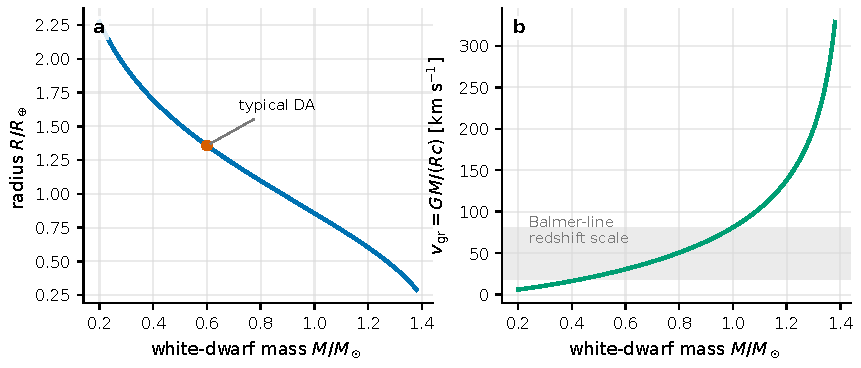
\includegraphics[width=0.94\linewidth]{figures/generated/chapter_11/ch11_white_dwarf_mass_radius.pdf}
\caption{白矮星质量增加时半径变小，靠近 Chandrasekhar 极限时收缩更快。右图把同一质量半径关系换成光谱中可测的引力红移速度 \(v_{\rm gr}=GM/(Rc)\)，典型 DA 白矮星的 Balmer 线红移是几十 \(\mathrm{km\,s^{-1}}\)，已经接近或超过普通恒星大气运动的速度尺度。}
\label{fig:chapter-11-wd-mr}
\end{figure}

质量半径关系可以通过几类数据进入观测。食双星的持续时间和径向速度给出 \(R/a\)、倾角和质量函数；视差加光谱能量分布可用 \(F_\lambda=(R/d)^2 H_\lambda(T_{\rm eff},\log g)\) 推出半径；谱线红移还能给出引力红移速度，
\begin{equation}
  v_{\rm gr}=\frac{GM}{Rc}
  \simeq 31.8\,\mathrm{km\,s^{-1}}
  \left(\frac{M}{0.6\,M_\odot}\right)
  \left(\frac{0.012\,R_\odot}{R}\right).
  \label{eq:ch11-05}
\end{equation}
\begin{formulaexplain}
\(v_{\rm gr}\) 是引力红移速度，正比于 \(M/R\)。谱线红移因此把白矮星质量半径关系变成可测速度，但必须扣除系统运动和线形成效应。
\end{formulaexplain}
这里 \(v_{\rm gr}\) 是谱线相对系统速度的红移。单个目标的系统速度、对流线移和 Stark 位移会污染这个量，所以大样本工作常把 Gaia 半径、SDSS 光谱线心和运动学模型一起平均。白矮星角直径本身很小，
\begin{equation}
  \theta_{\rm WD}=\frac{2R}{d}
  \simeq 11\,\mu{\rm as}
  \left(\frac{R}{0.012\,R_\odot}\right)
  \left(\frac{10\,{\rm pc}}{d}\right),
  \label{eq:ch11-06}
\end{equation}
\begin{formulaexplain}
\(\theta_{\rm WD}\) 是白矮星角直径，\(R\) 是半径，\(d\) 是距离。即使近到 \(10\,{\rm pc}\)，典型角尺度也只有微角秒，难以直接成像。
\end{formulaexplain}
所以即使在 \(10\,\mathrm{pc}\) 以内，普通光学成像也无法直接分辨。更可行的入口是把高速光度、偏振、谱线速度和相位信息保留在同一张事件表中。

\section{磁白矮星怎样把吸积几何写进相位和偏振}

磁白矮星把白矮星结构问题和光子统计问题连在一起。孤立磁白矮星的表面磁场可从 \(10^6\) 到 \(10^9\,\mathrm{G}\)，吸积系统中的极和中介极常见场强为 \(1-200\,\mathrm{MG}\)。磁矩写成
\begin{equation}
  \mu = B_* R_{\rm WD}^3
  \simeq 5.1\times10^{33}\,\mathrm{G\,cm^3}
  \left(\frac{B_*}{10\,{\rm MG}}\right)
  \left(\frac{R_{\rm WD}}{8\times10^8\,{\rm cm}}\right)^3 .
  \label{eq:ch11-07}
\end{equation}
\begin{formulaexplain}
\(\mu\) 是白矮星磁矩，\(B_*\) 是表面磁场，\(R_{\rm WD}\) 是半径。磁矩越大，磁场越能在更远处控制吸积流。
\end{formulaexplain}
这里 \(B_*\) 是白矮星表面磁场。给定 \(\mu\)、质量 \(M\) 和吸积率 \(\dot M\)，磁层半径的常用标度是
\begin{equation}
  r_m \simeq k
  \left(\frac{\mu^4}{2GM\dot M^2}\right)^{1/7},
  \label{eq:ch11-08}
\end{equation}
\begin{formulaexplain}
\(r_m\) 是磁层半径，\(k\) 是几何因子，\(\dot M\) 是吸积率。磁矩增强会推大磁层，吸积率升高会把磁层压向白矮星。
\end{formulaexplain}
其中 \(k\) 是几何因子，通常为 \(0.5-1\) 量级；\(\dot M\) 在激变变星中可从 \(10^{-11}\) 到 \(10^{-8}\,M_\odot\,{\rm yr^{-1}}\)。若 \(r_m\) 小于共转半径
\begin{equation}
  r_{\rm co}=\left(\frac{GM}{\Omega_s^2}\right)^{1/3},
  \label{eq:ch11-09}
\end{equation}
\begin{formulaexplain}
\(r_{\rm co}\) 是共转半径，\(\Omega_s\) 是白矮星自转角速度。在这个半径处，磁场共转角速度与 Kepler 轨道角速度相等。
\end{formulaexplain}
物质可以较顺利地沿磁力线落到磁极；若 \(r_m\) 接近或超过 \(r_{\rm co}\)，白矮星自转会把部分物质抛出或改变吸积流形态。中介极中 \(P_{\rm spin}/P_{\rm orb}\) 常在 \(0.01-0.6\)，极系统接近同步，\(P_{\rm spin}\simeq P_{\rm orb}\) \citep{1970ApJ...160L.147A,2000PASP..112..873W,1991MNRAS.249..460W,2008ApJ...672..524N}。

\begin{figure}[tbp]
\centering
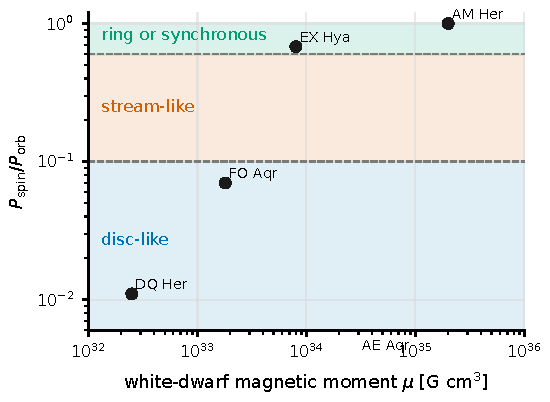
\includegraphics[width=0.78\linewidth]{figures/generated/chapter_11/ch11_magnetic_cv_flow_map.pdf}
\caption{磁激变变星的吸积流主要由白矮星磁矩和自转相对轨道的快慢决定。低 \(P_{\rm spin}/P_{\rm orb}\) 系统容易形成盘状流，中间区域常出现磁控流，接近同步或高比值系统会转向环状、流状或极系统几何；这些几何会直接改变光变相位、圆偏振和相关函数。}
\label{fig:chapter-11-mcv-map}
\end{figure}

吸积光度的数量级来自引力势能释放：
\begin{equation}
  L_{\rm acc}\simeq \frac{GM\dot M}{R_{\rm WD}}
  \simeq 1.0\times10^{33}\,\mathrm{erg\,s^{-1}}
  \left(\frac{M}{0.8\,M_\odot}\right)
  \left(\frac{\dot M}{10^{-10}M_\odot\,{\rm yr^{-1}}}\right)
  \left(\frac{8\times10^8\,{\rm cm}}{R_{\rm WD}}\right)
  \label{eq:ch11-10}
\end{equation}
\begin{formulaexplain}
\(L_{\rm acc}\) 是吸积光度，来自单位时间释放的引力势能。它给出磁激变变星可用光子率的数量级，实际光学只接收其中一部分。
\end{formulaexplain}
估算。光学波段只看到其中一部分，通常是盘、热斑、柱状冲击区、回照面和 cyclotron 辐射的混合。偏振能把 cyclotron 成分挑出来：圆偏振的符号随自转相位翻转时，通常表明视线穿过不同磁极或不同磁场投影；线偏振和总光变不同步时，强度峰和磁场几何峰往往不是同一个区域。

\Needspace{12\baselineskip}
事件表分析可以按自转相位或轨道相位分箱。令 \(\phi_s\) 是白矮星自转相位，\(I_{\phi_s}(t)\) 是该相位窗内的光子计数率，则
\begin{equation}
  g^{(2)}_{\phi_s}(\tau)=
  \frac{\langle I_{\phi_s}(t)I_{\phi_s}(t+\tau)\rangle}
  {\langle I_{\phi_s}(t)\rangle^2}
  \label{eq:ch11-11}
\end{equation}
\begin{formulaexplain}
\(g^{(2)}_{\phi_s}(\tau)\) 是固定自转相位窗内的二阶强度相关。它把同一磁极或吸积流片段在延迟 \(\tau\) 上的短时记忆提取出来。
\end{formulaexplain}
测的是同一个磁极或同一段吸积流在延迟 \(\tau\) 上的强度记忆。若 \(\tau\) 是毫秒到秒，信号可能来自冲击区冷却、磁控团块或探测器死时间；若 \(\tau\) 是几十秒到分钟，通常更像经典 flickering 或大气透明度变化。公式中的平均应在相同相位窗、相同能段和相同偏振通道内完成，否则轨道调制会被误认为短时相关。

\section{中子星怎样把磁层写进相位事件表}

中子星的半径只有 \(10-14\,\mathrm{km}\)，质量却常在 \(1.2-2.2\,M_\odot\)。自转把磁层切成相位坐标，最基本的长度是光柱半径
\begin{equation}
  R_{\rm LC}=\frac{c}{\Omega}=\frac{cP}{2\pi}
  \simeq 1.6\times10^3\,\mathrm{km}
  \left(\frac{P}{33\,{\rm ms}}\right).
  \label{eq:ch11-12}
\end{equation}
\begin{formulaexplain}
\(R_{\rm LC}\) 是光柱半径，\(P\) 是自转周期，\(\Omega\) 是角速度。它标出刚性共转达到光速的尺度，也是开放磁力线的基本边界。
\end{formulaexplain}
这里 \(P\) 是自转周期，Crab 脉冲星 \(P\simeq33\,\mathrm{ms}\)，毫秒脉冲星 \(P\simeq1.5-10\,\mathrm{ms}\)，磁星常为 \(2-12\,\mathrm{s}\)。在 \(R_{\rm LC}\) 之外，刚性共转需要超过光速，所以开放磁力线、粒子加速和高能辐射都要在这个尺度内组织。脉冲星发现和旋转中子星解释确立了这套图像，Crab 又把旋转能损失和超新星遗迹联系在一起 \citep{1968Natur.217..709H,1968Natur.218..731G,1968Natur.219..145P,1972ApJ...175..217B}。

\begin{figure}[tbp]
\centering
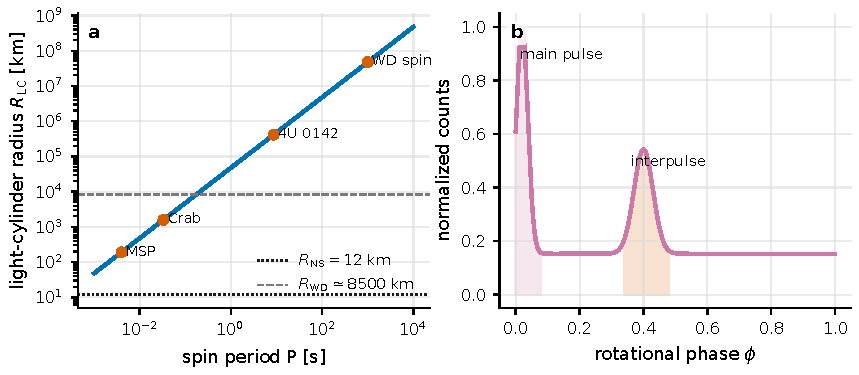
\includegraphics[width=0.94\linewidth]{figures/generated/chapter_11/ch11_light_cylinder_phase.pdf}
\caption{光柱半径随自转周期线性增加。毫秒脉冲星的光柱只有几十到几百公里，Crab 约 \(1.6\times10^3\,\mathrm{km}\)，磁星则可到 \(10^5\,\mathrm{km}\) 以上。右图是 Crab 型相位折叠轮廓，主脉冲和 interpulse 的相位窗决定哪些光子进入后续的强度相关或偏振统计。}
\label{fig:chapter-11-light-cylinder}
\end{figure}

磁偶极估算给表面赤道场
\begin{equation}
  B_{\rm dip}\simeq 3.2\times10^{19}(P\dot P)^{1/2}\,\mathrm{G},
  \label{eq:ch11-13}
\end{equation}
\begin{formulaexplain}
\(B_{\rm dip}\) 是由自转慢化估算的偶极磁场，\(P\) 和 \(\dot P\) 来自计时。它把事件到达时间中的慢化率换成磁场标度。
\end{formulaexplain}
\Needspace{12\baselineskip}
其中 \(P\) 用秒，\(\dot P\) 是无量纲的 \(\mathrm{s\,s^{-1}}\)。普通年轻脉冲星常在 \(10^{11}-10^{13}\,\mathrm{G}\)，磁星可到 \(10^{14}-10^{15}\,\mathrm{G}\)。旋转能损失率写成
\begin{equation}
  \dot E = 4\pi^2 I\frac{\dot P}{P^3},
  \qquad I\simeq10^{45}\,\mathrm{g\,cm^2}.
  \label{eq:ch11-14}
\end{equation}
\begin{formulaexplain}
\(\dot E\) 是自转能损失率，\(I\) 是转动惯量。它衡量脉冲星可用于驱动磁层辐射和星云的能量预算。
\end{formulaexplain}
Crab 的 \(\dot E\) 是 \(10^{38}\,\mathrm{erg\,s^{-1}}\) 量级，足以驱动从射电到 \(\gamma\) 射线的脉冲和星云辐射 \citep{1984ApJ...283..279H,1992ApJ...397..187B,2001A&A...378..918K,2008ApJ...680.1378H}。

事件表进入脉冲星分析时，每个光子先做太阳系质心改正，再用时序星历折叠：
\begin{equation}
  \phi_i =
  \left[
  \nu(t_i-t_0)+\frac{1}{2}\dot\nu(t_i-t_0)^2
  +\frac{1}{6}\ddot\nu(t_i-t_0)^3+\cdots
  \right]\bmod 1 .
  \label{eq:ch11-15}
\end{equation}
\begin{formulaexplain}
\(\phi_i\) 是第 \(i\) 个光子的自转相位，\(\nu,\dot\nu,\ddot\nu\) 是频率及其导数。这个折叠式把到达时间表变成相位事件表。
\end{formulaexplain}
这里 \(t_i\) 是第 \(i\) 个光子的质心到达时刻，单位秒；\(\nu=1/P\) 是自转频率；\(\dot\nu\) 和 \(\ddot\nu\) 描述慢化和 glitch 后恢复。Crab 的主脉冲宽度约占相位 \(0.04-0.05\)，射电巨脉冲可窄到微秒量级。若把巨射电脉冲发生的周期挑出来，光学主脉冲平均会增强约 \(3\%\)，而脉冲形状和到达相位基本不变；ARCONS 的能量分辨光子计数进一步显示，早到的巨射电脉冲对应的光学增强可达十几到二十几个百分点 \citep{2003Sci...301..493S,2013ApJ...779L..12S}。这些结果把相干射电爆发和非相干光学辐射接到同一部分磁层等离子体上。

相位分辨二阶相关可写为
\begin{equation}
  g^{(2)}_{ab}(\tau|\Phi)=
  \frac{\langle n_a(t,\Phi)n_b(t+\tau,\Phi)\rangle}
  {\langle n_a(t,\Phi)\rangle\langle n_b(t,\Phi)\rangle},
  \label{eq:ch11-16}
\end{equation}
\begin{formulaexplain}
\(g^{(2)}_{ab}(\tau|\Phi)\) 是相位窗 \(\Phi\) 内两个通道 \(a,b\) 的相关。它可比较不同能段、偏振或望远镜在同一脉冲相位的同步涨落。
\end{formulaexplain}
其中 \(a,b\) 可以是能段、偏振通道或不同望远镜，\(\Phi\) 是主脉冲、bridge 或 interpulse 相位窗。对 Crab 这样的亮目标，\(\tau\) 可以推进到微秒至毫秒；对更暗的光学脉冲星，最先能做的通常是相位窗内的光度和偏振堆叠，离单脉冲统计还有距离 \citep{1996ApJ...468..779M,2000ApJ...537..861S,2009MNRAS.397..103S}。

\section{强磁场偏振怎样检验传播中的量子效应}

强磁场偏振的基本标尺是 QED 临界场
\begin{equation}
  B_Q=\frac{m_e^2c^3}{e\hbar}
  =4.414\times10^{13}\,\mathrm{G}.
  \label{eq:ch11-17}
\end{equation}
\begin{formulaexplain}
\(B_Q\) 是 QED 临界磁场，在这个场强下电子回旋能量接近静能。磁星表面磁场接近或超过它，真空传播不再像普通介质外的空白背景。
\end{formulaexplain}
当 \(B\ll B_Q\) 且光子能量远低于 \(m_ec^2\) 时，Heisenberg-Euler 有效理论给真空折射率差的弱场近似
\begin{equation}
  \Delta n \simeq
  \frac{\alpha_{\rm fs}}{30\pi}
  \left(\frac{B_\perp}{B_Q}\right)^2 ,
  \label{eq:ch11-18}
\end{equation}
\begin{formulaexplain}
\(\Delta n\) 是两个偏振正常模的折射率差，\(B_\perp\) 是横向磁场。弱场近似显示双折射效应随 \(B_\perp^2\) 快速增强。
\end{formulaexplain}
\Needspace{13\baselineskip}
其中 \(B_\perp\) 是垂直于光线方向的磁场分量，\(\alpha_{\rm fs}\) 是精细结构常数。磁星表面 \(B\sim10^{14}-10^{15}\,\mathrm{G}\)，弱场公式不能直接当作精确模型，但它给出偏振对强场敏感的原因：两个正常模的相位差沿路径积累，
\begin{equation}
  \Delta \Phi(E)=\frac{E}{\hbar c}\int \Delta n(s)\,ds .
  \label{eq:ch11-19}
\end{equation}
\begin{formulaexplain}
\(\Delta\Phi(E)\) 是两个偏振模积累的相位差，\(E\) 是光子能量。能量越高、路径上 \(\Delta n\) 越大，偏振传播效应越明显。
\end{formulaexplain}
这里 \(E\) 是光子能量，X 射线偏振仪常在 \(2-8\,\mathrm{keV}\) 工作；积分沿光路进行。若传播是绝热的，偏振矢量会随局部磁场方向转动，直到偏振限制半径之后冻结。这个物理图像来自强场 QED、磁层传播和中子星表面辐射模型的组合 \citep{1936ZPhy...98..714H,1971AnPhy..67..599A,2000MNRAS.311..555H,2002PhRvD..66b3002H,2003MNRAS.342..134H}。

\Needspace{12\baselineskip}
偏振观测需要同时报告强度、偏振度和偏振角。线偏振的事件估计通常从调制角 \(\eta_i\) 出发，
\begin{equation}
  I=\sum_i w_i,\qquad
  Q=\sum_i w_i\cos 2\eta_i,\qquad
  U=\sum_i w_i\sin 2\eta_i,
  \label{eq:ch11-20}
\end{equation}
\begin{formulaexplain}
\(I,Q,U\) 是 Stokes 量，\(\eta_i\) 是单个事件的调制角，\(w_i\) 是权重。偏振仪把许多光子的方位角累加成线偏振信号。
\end{formulaexplain}
然后得到
\begin{equation}
  p=\frac{\sqrt{Q^2+U^2}}{I},\qquad
  \psi=\frac{1}{2}\arctan2(U,Q).
  \label{eq:ch11-21}
\end{equation}
\begin{formulaexplain}
\(p\) 是线偏振度，\(\psi\) 是偏振角。\(Q,U\) 的矢量长度给偏振强度，方向给天空上的偏振角。
\end{formulaexplain}
这里 \(p\) 是线偏振度，取值 \(0-1\)；\(\psi\) 是偏振角；\(w_i\) 包含仪器调制因子、背景权重和有效面积权重。光学偏振测量 RX J1856.5-3754 得到 \(p=16.43\%\pm5.26\%\)，源本身 \(V\simeq25.5\)，前景偏振和仪器偏振都要逐项扣除；这类测量和热表面模型相比，支持真空双折射会减少不同表面区域的偏振相消 \citep{2015MNRAS.454.3254T,2016MNRAS.459.3585G,2017MNRAS.465..492M}。

\begin{figure}[tbp]
\centering
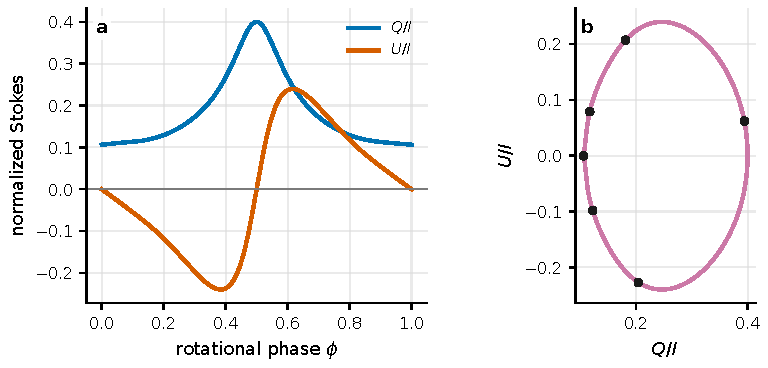
\includegraphics[width=0.92\linewidth]{figures/generated/chapter_11/ch11_stokes_qu_track.pdf}
\caption{旋转磁几何会把偏振角变化投影成 \(Q/I\) 和 \(U/I\) 的相位曲线。左图显示同一相位事件表给出的两个 Stokes 分量，右图显示对应的 Q-U 轨迹；轨迹形状比单独的偏振度更能暴露几何退化和仪器串扰。}
\label{fig:chapter-11-stokes}
\end{figure}

相位依赖的偏振角常用旋转矢量模型作第一近似：
\begin{equation}
  \tan(\psi-\psi_0)=
  \frac{\sin\alpha \sin(\phi-\phi_0)}
  {\sin\zeta\cos\alpha-\cos\zeta\sin\alpha\cos(\phi-\phi_0)} .
  \label{eq:ch11-22}
\end{equation}
\begin{formulaexplain}
\(\psi\) 是偏振角，\(\alpha\) 是磁轴倾角，\(\zeta\) 是视线倾角，\(\phi\) 是自转相位。旋转矢量模型把相位上的偏振角摆动翻译成磁层几何。
\end{formulaexplain}
这里 \(\alpha\) 是磁轴和自转轴夹角，\(\zeta\) 是视线和自转轴夹角，\(\phi\) 是自转相位，\(\psi_0\) 和 \(\phi_0\) 是零点。这个公式最早用于射电脉冲星偏振几何；在磁星 X 射线中，它只是低维几何骨架，因为表面辐射、共振 cyclotron 散射和真空双折射会一起改变 \(p(E,\phi)\) 和 \(\psi(E,\phi)\) \citep{1969ApL.....3..225R,2018ApJ...854...98W,2011ApJ...730..131F}。

\begin{figure}[tbp]
\centering
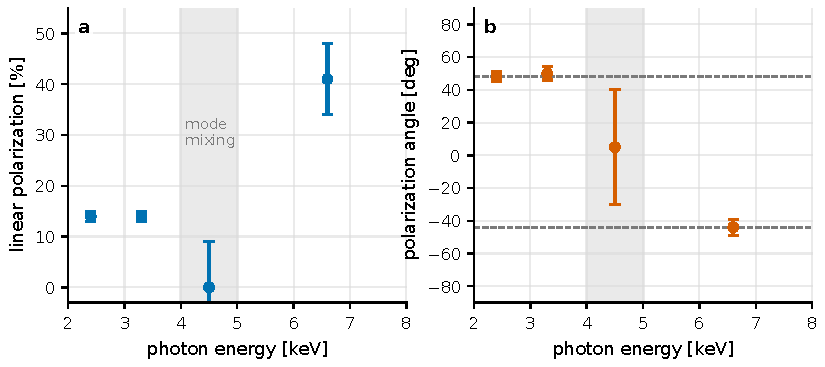
\includegraphics[width=0.92\linewidth]{figures/generated/chapter_11/ch11_birefringence_energy.pdf}
\caption{IXPE 对磁星 4U 0142+61 的结果可以看成两个偏振正常模在能量上的切换。低能 \(2-4\,\mathrm{keV}\) 偏振度约 \(14\%\)，高能 \(5.5-8\,\mathrm{keV}\) 升到约 \(41\%\)，而 \(4-5\,\mathrm{keV}\) 附近偏振度接近最低可探测偏振，偏振角发生约 \(90^\circ\) 翻转。}
\label{fig:chapter-11-birefringence}
\end{figure}

4U 0142+61 是一个具体例子。IXPE 在 \(2-8\,\mathrm{keV}\) 看到总线偏振度 \(12\%\pm1\%\)，低能 \(2-4\,\mathrm{keV}\) 为 \(14\%\pm1\%\)，高能 \(5.5-8\,\mathrm{keV}\) 为 \(41\%\pm7\%\)，中间 \(4-5\,\mathrm{keV}\) 附近偏振度降到灵敏度附近并伴随偏振角约 \(90^\circ\) 翻转。源的自转周期 \(P=8.69\,\mathrm{s}\)，磁场 \(B\sim10^{14}\,\mathrm{G}\)，软 X 射线有 \(kT\sim0.5-1\,\mathrm{keV}\) 黑体成分，硬尾可延伸到几十甚至上百 keV。解释这组数据时，低能 O 模、硬尾 X 模、表面凝聚态或薄大气、以及共振 Compton 散射都可能参与；单个高偏振点还不足以单独构成真空双折射探测 \citep{2022Sci...378..646T,2023A&A...674L..10C,2023MNRAS.519.3681F}。

\section{热斑光变怎样反推中子星半径}

中子星半径不能直接量角直径，只能从光变形状、能谱和相对论传播反推。紧致度
\begin{equation}
  u=\frac{2GM}{Rc^2}
  \simeq 0.345
  \left(\frac{M}{1.4\,M_\odot}\right)
  \left(\frac{12\,{\rm km}}{R}\right)
  \label{eq:ch11-23}
\end{equation}
\begin{formulaexplain}
\(u\) 是中子星紧致度，等于 Schwarzschild 半径与真实半径之比。\(u\) 越大，引力光弯曲越强，热斑光变振幅越容易被抹平。
\end{formulaexplain}
决定光弯曲强度。\(u\) 越大，背面热斑越容易被弯到视线中，脉冲振幅越小、轮廓越平滑。一个常用近似把发射角 \(\alpha\) 和斑点相对视线的中心角 \(\psi\) 联系起来：
\begin{equation}
  \cos\alpha \simeq u+(1-u)\cos\psi .
  \label{eq:ch11-24}
\end{equation}
\begin{formulaexplain}
\(\alpha\) 是光子离开表面时的发射角，\(\psi\) 是斑点中心相对视线的角距。这个近似把弯曲后的可见性写成紧致度的简单函数。
\end{formulaexplain}
它适用于 Schwarzschild 外部时空、慢自转或中等自转的标度估算；快速毫秒脉冲星还要加入 Doppler boost、像差、时延、星体扁率和大气束射 \citep{2002ApJ...566L..85B,2019AIPC.2127b0008W}。

\begin{figure}[tbp]
\centering
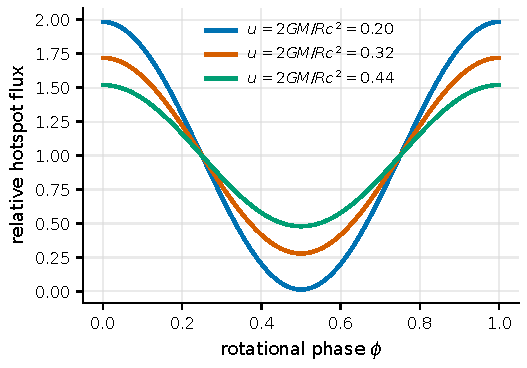
\includegraphics[width=0.78\linewidth]{figures/generated/chapter_11/ch11_hotspot_lightcurve.pdf}
\caption{热斑光变对紧致度很敏感。低紧致度时，斑点转到背面后贡献迅速消失，脉冲振幅大；高紧致度时，引力光弯曲让更大范围的表面可见，光变谷底被抬高。半径推断利用这种轮廓变化，并与质量、倾角、热斑位置和大气束射一起拟合。}
\label{fig:chapter-11-hotspot}
\end{figure}

对一个带能谱的热斑，探测器中第 \(j\) 个能道、第 \(k\) 个相位 bin 的期望计数可写成
\begin{equation}
  \lambda_{jk}(\Theta)=
  T\int dE\,
  R_j(E)\,
  \left[
  F_E(\phi_k;\Theta)+B_E
  \right].
  \label{eq:ch11-25}
\end{equation}
\begin{formulaexplain}
\(\lambda_{jk}\) 是能道 \(j\)、相位 bin \(k\) 的期望计数，\(R_j(E)\) 是仪器响应，\(F_E\) 是热斑模型通量。它把天体模型变成探测器中的预期事件数。
\end{formulaexplain}
\Needspace{13\baselineskip}
这里 \(T\) 是曝光时间，\(R_j(E)\) 是有效面积和能量重分布组成的响应，\(F_E\) 是模型热斑通量，\(B_E\) 是背景，\(\Theta\) 包含 \(M,R\)、距离、倾角、斑点经纬度、斑点角半径、温度和大气参数。实际计数服从 Poisson 统计：
\begin{equation}
  \ln{\cal L}(\Theta)=
  \sum_{j,k}\left[
  N_{jk}\ln\lambda_{jk}(\Theta)-\lambda_{jk}(\Theta)-\ln(N_{jk}!)
  \right].
  \label{eq:ch11-26}
\end{equation}
\begin{formulaexplain}
\(\ln{\cal L}\) 是 Poisson 对数似然，\(N_{jk}\) 是观测计数。半径推断就是寻找让所有能道和相位 bin 的 \(\lambda_{jk}\) 最接近事件表的参数 \(\Theta\)。
\end{formulaexplain}
NICER 对 PSR J0030+0451 和 PSR J0740+6620 的半径结果属于这种事件表建模。J0740 的分析把 NICER 事件表、XMM-Newton 成像光谱背景、以及射电计时给出的质量和距离先验联合起来；Riley 等得到 \(R=12.39^{+1.30}_{-0.98}\,\mathrm{km}\)、\(M=2.072^{+0.067}_{-0.066}M_\odot\)，Miller 等得到相容但方法不同的半径约束。J0030 的两套独立分析也显示，热斑几何可能包含复杂的多极磁场结构 \citep{2019ApJ...887L..21R,2019ApJ...887L..24M,2021ApJ...918L..27R,2021ApJ...918L..28M}。


\chapter{黑洞、吸积盘和 photon ring}
\label{chap:12}

\begin{chapteropening}
黑洞没有可见固体表面，观测到的是它周围物质和光路的结构。吸积盘给出连续谱和随机光变，宽线区把光变延迟转成物理半径，喷流把磁场和相对论运动投影成强偏振，photon ring 把强引力多路径写进长基线可见度和时间延迟。光子事件表中的时间、频率、偏振和干涉相位应尽量保留下来，这些坐标决定了强引力、等离子体和仪器效应能否被分开估计。
\end{chapteropening}

\section{黑洞尺度怎样定下所有坐标}

黑洞问题的自然单位由质量决定：
\begin{equation}
  r_g=\frac{GM}{c^2},\qquad
  t_g=\frac{GM}{c^3},\qquad
  \theta_g=\frac{r_g}{D}.
  \label{eq:ch12-01}
\end{equation}
\begin{formulaexplain}
\(r_g\) 是引力半径，\(t_g\) 是对应光行时，\(\theta_g\) 是角尺度。黑洞质量一旦给定，长度、时间和天空角尺度就都有了共同标尺。
\end{formulaexplain}
这里 \(r_g\) 是引力半径，单位通常用 \(\mathrm{km}\) 或 \(\mathrm{cm}\)；\(t_g\) 是光穿过一个 \(r_g\) 所需的时间；\(D\) 是距离。数值上
\begin{equation}
  r_g=1.477\,{\rm km}\left(\frac{M}{M_\odot}\right),\qquad
  t_g=4.93\,\mu{\rm s}\left(\frac{M}{M_\odot}\right).
  \label{eq:ch12-02}
\end{equation}
\begin{formulaexplain}
这组数值把质量直接换成公里和微秒。它说明同一无量纲吸积过程在 Sgr A* 和 M87* 上会有完全不同的观测时间尺度。
\end{formulaexplain}
Sgr A* 的 \(M\simeq4\times10^6\,M_\odot\)，所以 \(t_g\simeq20\,\mathrm{s}\)，ISCO 量级的变化可以在几分钟内出现。M87* 的 \(M=(6.5\pm0.7)\times10^9\,M_\odot\)，\(t_g\simeq3.2\times10^4\,\mathrm{s}\)，同样的无量纲过程会被拉长到小时到天 \citep{2019ApJ...875L...1E,2019ApJ...875L...6E,2022ApJ...930L..12E}。

黑洞阴影的角直径可以粗略写成
\begin{equation}
  d_{\rm sh}\simeq \kappa\,\theta_g,\qquad \kappa\simeq 10.4 ,
  \label{eq:ch12-03}
\end{equation}
\begin{formulaexplain}
\(d_{\rm sh}\) 是黑洞阴影角直径，\(\kappa\) 是从引力半径到阴影直径的无量纲系数。EHT 测到的环尺度本质上是 \(\theta_g\) 的放大版本。
\end{formulaexplain}
其中 \(\kappa\) 对 Kerr 黑洞的自旋和倾角只有百分之几到十来个百分点的变化。EHT 在 \(1.3\,\mathrm{mm}\) 看到 M87* 的非对称环直径为 \(42\pm3\,\mu{\rm as}\)，中心亮度压低超过十倍；Sgr A* 的厚环直径为 \(51.8\pm2.3\,\mu{\rm as}\)，但源在观测夜内有明显分钟到小时级结构变化 \citep{2019ApJ...875L...4E,2019ApJ...875L...5E,2022ApJ...930L..14E,2022ApJ...930L..15E}。

\begin{figure}[tbp]
\centering
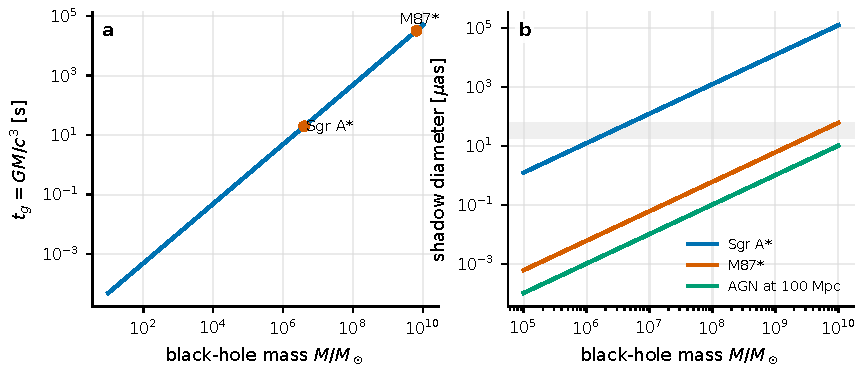
\includegraphics[width=0.94\linewidth]{figures/generated/chapter_12/ch12_black_hole_scales.pdf}
\caption{黑洞时间尺度和角尺度都由质量线性控制。Sgr A* 和 M87* 的质量相差约 \(10^3\)，但距离也相差约 \(10^3\)，所以二者的阴影角直径都在几十微角秒；时间尺度却完全不同，Sgr A* 可以在一次 VLBI 扫描内改变，M87* 的结构更接近静态。}
\label{fig:chapter-12-scales}
\end{figure}

事件表里，黑洞观测的基本坐标扩展为
\[
  (t_i,\nu_i,{\bf b}_i,\eta_i,w_i),
\]
其中 \(t_i\) 是到达时间，\(\nu_i\) 是频率或能道，\({\bf b}_i\) 是投影基线，\(\eta_i\) 是偏振调制角或 Stokes 通道，\(w_i\) 是权重。EHT 的复可见度、GRAVITY 的差分相位、光学监测的光变和偏振巡天都可以看成这张事件表的不同投影。投影前保留时间和偏振，才能比较吸积流变化、喷流扰动和强引力多路径。

\section{吸积盘怎样产生连续谱和随机变异}

标准薄盘把引力势能局部转化为辐射通量：
\begin{equation}
  F(R)=\frac{3GM\dot M}{8\pi R^3}
  \left[1-\left(\frac{R_{\rm in}}{R}\right)^{1/2}\right],
  \label{eq:ch12-04}
\end{equation}
\begin{formulaexplain}
\(F(R)\) 是薄盘单位面积辐射通量，\(\dot M\) 是吸积率，\(R_{\rm in}\) 是内边界。它把引力能释放分配到不同盘半径。
\end{formulaexplain}
其中 \(R\) 是盘半径，\(\dot M\) 是吸积率，\(R_{\rm in}\) 是内边界，常取几倍 \(r_g\) 量级。若盘在局部近似黑体，温度为
\begin{equation}
  T(R)=\left[\frac{F(R)}{\sigma_{\rm SB}}\right]^{1/4}.
  \label{eq:ch12-05}
\end{equation}
\begin{formulaexplain}
\(T(R)\) 是盘的局部有效温度，\(\sigma_{\rm SB}\) 是 Stefan--Boltzmann 常数。薄盘连续谱的颜色来自不同半径黑体温度的叠加。
\end{formulaexplain}
远离内边界时 \(T\propto R^{-3/4}\)，于是某个波长主导的半光半径满足
\begin{equation}
  R_\lambda \propto (M\dot M)^{1/3}\lambda^{4/3}.
  \label{eq:ch12-06}
\end{equation}
\begin{formulaexplain}
\(R_\lambda\) 是波长 \(\lambda\) 附近主要发光的盘半径。波长越长，来自越外层；质量和吸积率越大，盘的同一颜色区域也越大。
\end{formulaexplain}
对 \(M\sim10^8\,M_\odot\)、\(L/L_{\rm Edd}\sim0.1\) 的类星体，光学和近紫外连续谱常来自 \(0.1-10\) light-day 量级的半径。微透镜和多波段延迟经常给出比最简单薄盘更大的光学盘，这就是 inhomogeneous disk 模型和再处理模型被反复讨论的原因 \citep{1973A&A....24..337S,2006ApJ...642...87P,2011ApJ...727L..24D}。

\begin{figure}[tbp]
\centering
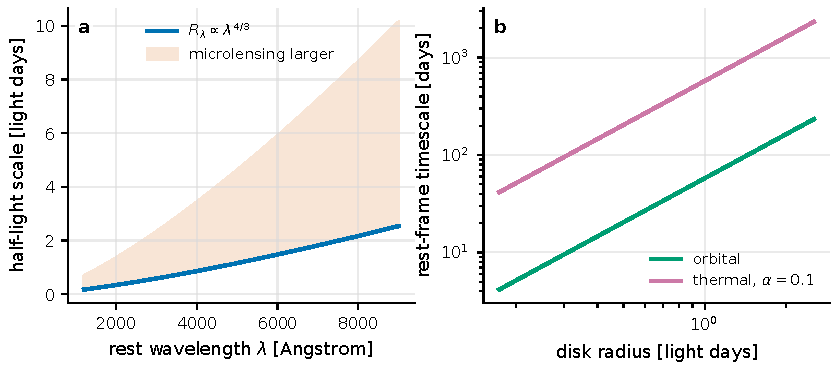
\includegraphics[width=0.94\linewidth]{figures/generated/chapter_12/ch12_accretion_disk_radii.pdf}
\caption{薄盘标度给出 \(R_\lambda\propto\lambda^{4/3}\)。左图的橙色区域表示微透镜和部分连续谱延迟常暗示的更大光学发光面积；右图比较同一半径上的轨道时间和热时间，若 \(\alpha\simeq0.1\)，热时间约为轨道时间的十倍。}
\label{fig:chapter-12-disk}
\end{figure}

盘上一个半径的动力学和热时间分别可估为
\begin{equation}
  t_{\rm orb}=2\pi\left(\frac{R^3}{GM}\right)^{1/2},\qquad
  t_{\rm th}\simeq \frac{t_{\rm orb}}{\alpha}.
  \label{eq:ch12-07}
\end{equation}
\begin{formulaexplain}
\(t_{\rm orb}\) 是 Kepler 轨道时间，\(t_{\rm th}\) 是热时间，\(\alpha\) 是粘滞参数。光变能否快速响应，取决于扰动落在哪个盘时间尺度上。
\end{formulaexplain}
\Needspace{12\baselineskip}
\(\alpha\) 是 Shakura-Sunyaev 粘滞参数，常用 \(0.01-0.3\) 的范围做估计。对 AGN 光学盘，\(t_{\rm orb}\) 可以是几十天到几年，\(t_{\rm th}\) 更长。大样本光学光变常用阻尼随机游走描述：
\begin{equation}
  C(\tau)=\sigma^2\exp\left(-\frac{|\tau|}{\tau_d}\right),
  \qquad
  P(f)\propto\frac{1}{1+(2\pi f\tau_d)^2}.
  \label{eq:ch12-08}
\end{equation}
\begin{formulaexplain}
\(C(\tau)\) 是自协方差，\(P(f)\) 是功率谱，\(\tau_d\) 是阻尼时间。这个模型把随机盘光变写成一个会逐渐失忆的相关过程。
\end{formulaexplain}
这里 \(C(\tau)\) 是光变自协方差，\(\tau_d\) 是阻尼时间，单位通常是 rest-frame day；\(P(f)\) 是功率谱密度。观测上 \(\tau_d\) 和黑洞质量相关，超大质量黑洞常为数十到数百天，白矮星吸积盘也落在相近的质量缩放趋势上 \citep{1993ApJ...406..420M,2021Sci...373..789B,2016Natur.534...75M}。

\begin{figure}[tbp]
\centering
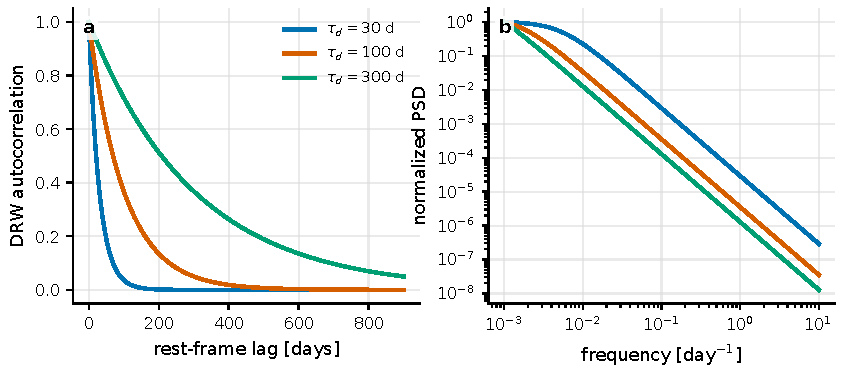
\includegraphics[width=0.94\linewidth]{figures/generated/chapter_12/ch12_variability_autocorrelation.pdf}
\caption{阻尼随机游走模型把随机光变写成一个相关时间。短 \(\tau_d\) 的光变很快失去记忆，功率谱较早转入 \(f^{-2}\) 衰减；长 \(\tau_d\) 的盘在更长时间上保持相关，低频平台延伸得更远。}
\label{fig:chapter-12-variability}
\end{figure}

对光子统计，吸积盘的难点是多模稀释。一个 \(10^8\,M_\odot\) AGN 的光学连续谱来自大量独立湍流区域和多个热时间，单一量子态的 bunching 信号会被空间、频率和时间模式平均掉。可测量的量更可能是相位或颜色条件下的过量相关，例如在一个 flare 前后比较 \(g^{(2)}(\tau)\) 的宽度，或把偏振通道分开看 turbulent cell 的寿命。平均亮度主要给出光子率和归一化；可探测性还受相干时间、采样窗口和经典涨落可建模程度控制。

\section{宽线区怎样把时间延迟和角位移合在一起}

宽线区的传统反响映射写成
\begin{equation}
  L(v,t)=\int \Psi(v,\tau)\,C(t-\tau)\,d\tau ,
  \label{eq:ch12-09}
\end{equation}
\begin{formulaexplain}
\(C(t)\) 是连续谱驱动光变，\(L(v,t)\) 是谱线响应，\(\Psi(v,\tau)\) 是转移函数。BLR 反响映射把时间延迟和速度结构一起编码。
\end{formulaexplain}
其中 \(C(t)\) 是连续谱光变，\(L(v,t)\) 是速度 \(v\) 处的谱线光变，\(\Psi(v,\tau)\) 是转移函数。延迟 \(\tau\) 对应 \(R\simeq c\tau\)，速度宽度给引力势中的轨道速度。经验上 H\(\beta\) 半径和 \(5100\text{\AA}\) 连续谱光度满足
\begin{equation}
  R_{\rm BLR}\simeq 33.7\,{\rm light\,days}
  \left[\frac{\lambda L_\lambda(5100\text{\AA})}{10^{44}\,\mathrm{erg\,s^{-1}}}\right]^{0.533}.
  \label{eq:ch12-10}
\end{equation}
\begin{formulaexplain}
\(R_{\rm BLR}\) 是宽线区半径，\(\lambda L_\lambda\) 是 \(5100\text{\AA}\) 连续谱光度。这个经验关系让单历元光谱也能估计 BLR 尺度。
\end{formulaexplain}
这个关系的散布来自宿主星光扣除、采样窗口、各向异性照明、线种差异和 BLR 几何差异。黑洞质量常写为
\begin{equation}
  M_{\rm BH}=f_{\rm vir}\frac{R_{\rm BLR}\Delta V^2}{G},
  \label{eq:ch12-11}
\end{equation}
\begin{formulaexplain}
\(M_{\rm BH}\) 是黑洞质量，\(\Delta V\) 是宽线速度宽度，\(f_{\rm vir}\) 是几何因子。它是用 BLR 半径和轨道速度做的 virial 质量估计。
\end{formulaexplain}
其中 \(\Delta V\) 是谱线宽度，\(f_{\rm vir}\) 吸收倾角和速度场几何。对 Seyfert，\(\tau\) 可以是几天到几十天；对亮类星体，\(\tau\) 可达数百天，监测窗口和季节间断会成为主要系统误差 \citep{1982ApJ...255..419B,1993PASP..105..247P,2013ApJ...767..149B}。

干涉相位给 BLR 另一种投影。若谱线某个速度通道的光心相对连续谱偏移 \(\boldsymbol{\delta\theta}(v)\)，基线 \({\bf B}\) 上的差分相位近似为
\begin{equation}
  \Delta\varphi(v)\simeq
  2\pi\frac{{\bf B}\cdot\boldsymbol{\delta\theta}(v)}{\lambda}.
  \label{eq:ch12-12}
\end{equation}
\begin{formulaexplain}
\(\Delta\varphi(v)\) 是速度通道的差分相位，\({\bf B}\) 是基线，\(\boldsymbol{\delta\theta}\) 是光心偏移。相位直接测的是谱线发光区的角位移投影。
\end{formulaexplain}
这里 \(\Delta\varphi\) 用弧度，\({\bf B}\) 用米，\(\lambda\) 用米，\(\boldsymbol{\delta\theta}\) 用弧度。GRAVITY 对 3C 273 的 Pa\(\alpha\) 谱线测到红蓝翼光心沿近似垂直喷流方向的梯度，模型给 \(R_{\rm BLR}=46\pm10\,\mu{\rm as}\)，对应约 \(145\) light-days，并得到接近 face-on 的厚盘旋转几何 \citep{2018Natur.563..657G}。

\begin{figure}[tbp]
\centering
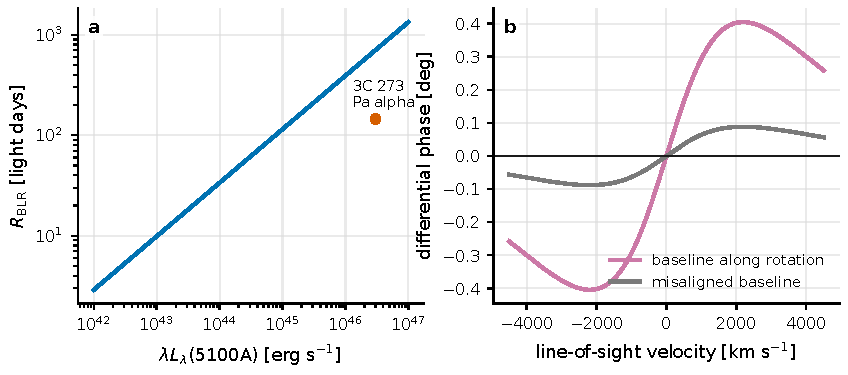
\includegraphics[width=0.94\linewidth]{figures/generated/chapter_12/ch12_blr_reverberation_interferometry.pdf}
\caption{BLR 的时间和角度信息互补。左图是 H\(\beta\) 半径-光度关系，时间延迟给物理半径；右图示意旋转 BLR 的红蓝翼会在基线上产生反号差分相位，基线若与旋转轴几何不匹配，相位振幅会被压低。}
\label{fig:chapter-12-blr}
\end{figure}

强度干涉若用于谱线区，测到的是窄带角结构的 \(|V|^2\)，与 GRAVITY 的差分相位不同。它更适合亮、低红移、宽线强、角尺度大的目标。设 BLR 半径 \(R_{\rm BLR}=100\) light-days，角直径为
\begin{equation}
  \theta_{\rm BLR}\simeq 2\frac{R_{\rm BLR}}{D_A}
  \simeq 11\,\mu{\rm as}
  \left(\frac{R_{\rm BLR}}{100\,{\rm light\,days}}\right)
  \left(\frac{100\,{\rm Mpc}}{D_A}\right),
  \label{eq:ch12-13}
\end{equation}
\begin{formulaexplain}
\(\theta_{\rm BLR}\) 是 BLR 角直径，\(D_A\) 是角直径距离。若时间延迟给物理半径、干涉给角半径，就能形成几何距离。
\end{formulaexplain}
这已经要求百米到公里级基线和非常高的光子通量。若同时有反响映射给 \(R_{\rm BLR}\) 和干涉给 \(\theta_{\rm BLR}\)，可以形成几何距离 \(D_A=2R_{\rm BLR}/\theta_{\rm BLR}\)，但误差会被倾角、BLR 各向异性、线区厚度和宿主污染放大。

\section{喷流偏振怎样把磁场几何带进光子统计}

旋转黑洞和磁通量可以给喷流供能。Blandford-Znajek 机制的常用标度是
\begin{equation}
  P_{\rm BZ}\sim \frac{\kappa}{4\pi c}\Phi_{\rm BH}^2\Omega_H^2,
  \label{eq:ch12-14}
\end{equation}
\begin{formulaexplain}
\(P_{\rm BZ}\) 是 Blandford--Znajek 喷流功率标度，\(\Phi_{\rm BH}\) 是黑洞磁通量，\(\Omega_H\) 是视界角速度。自旋和磁通量共同决定可抽取功率。
\end{formulaexplain}
其中 \(\Phi_{\rm BH}\) 是穿过黑洞的磁通量，\(\Omega_H\) 是视界角速度，\(\kappa\) 是与场结构有关的无量纲系数。对 M87* 这类低吸积率射电星系，EHT 偏振显示视界尺度附近存在有序磁场，和磁控吸积流及喷流功率的图像相容 \citep{1977MNRAS.179..433B,1979ApJ...232...34B,2021ApJ...910L..13E}。

喷流光学和近红外通常来自同步辐射。电子 Lorentz 因子 \(\gamma_e\) 在磁场 \(B\) 中的特征频率为
\begin{equation}
  \nu_{\rm syn}\simeq
  4.2\times10^6\,{\rm Hz}\,
  \frac{\delta}{1+z}
  \left(\frac{B}{1\,{\rm G}}\right)\gamma_e^2 ,
  \label{eq:ch12-15}
\end{equation}
\begin{formulaexplain}
\(\nu_{\rm syn}\) 是同步辐射特征频率，\(B\) 是磁场，\(\gamma_e\) 是电子 Lorentz 因子，\(\delta\) 是 Doppler 因子。它把观测频率换成喷流电子能量。
\end{formulaexplain}
其中 \(\delta\) 是 Doppler 因子，\(z\) 是红移。若 \(B\simeq0.1-1\,\mathrm{G}\)、\(\delta\simeq10\)，光学 \(\nu\sim5\times10^{14}\,\mathrm{Hz}\) 需要 \(\gamma_e\sim10^4\)。幂律电子 \(N(E)\propto E^{-p}\) 的最大线偏振度为
\begin{equation}
  \Pi_{\rm max}=\frac{p+1}{p+7/3},
  \label{eq:ch12-16}
\end{equation}
\begin{formulaexplain}
\(\Pi_{\rm max}\) 是理想同步辐射最大线偏振度，\(p\) 是电子能谱指数。实际偏振低于它，通常说明有多个磁场方向在视线内相加。
\end{formulaexplain}
对 \(p=2-3\)，\(\Pi_{\rm max}\simeq70\%-75\%\)。真实 blazar 通常只有几百分比到几十百分比，因为多个磁场胞元、冲击、剪切和湍流会把 Stokes 向量相加抵消。跨频触发时，光学偏振角旋转、\(\gamma\) 射线 flare 和射电 knot 抛射若时间相符，通常指向同一个喷流扰动穿过不同发光区 \citep{1995PASP..107..803U,2008Natur.452..966M}。

偏振分辨的二阶相关可以写成
\begin{equation}
  g^{(2)}_{QU}(\tau)=
  \frac{\langle \delta Q(t)\delta U(t+\tau)\rangle}
  {\sigma_Q\sigma_U},
  \label{eq:ch12-17}
\end{equation}
\begin{formulaexplain}
\(g^{(2)}_{QU}(\tau)\) 是两个 Stokes 涨落之间的归一化相关。它把喷流磁场方向变化写成可随延迟 \(\tau\) 测量的偏振统计。
\end{formulaexplain}
这个量描述磁场方向的随机过程在两个 Stokes 分量之间如何延迟。若 shock-in-jet 模型正确，\(Q,U\) 的相关时间应接近扰动穿过光学发光区的时间；若湍流胞元主导，相关函数会更快衰减，且在不同颜色上不完全同步。

\section{Photon ring 怎样进入图像、可见度和时间结构}

干涉仪测的是天空亮度的 Fourier 分量：
\begin{equation}
  V({\bf u})=\int I({\boldsymbol\theta})
  e^{-2\pi i{\bf u}\cdot{\boldsymbol\theta}}\,d^2\theta,
  \qquad {\bf u}=\frac{{\bf B}_\perp}{\lambda}.
  \label{eq:ch12-18}
\end{equation}
\begin{formulaexplain}
\(V({\bf u})\) 是复可见度，\(I({\boldsymbol\theta})\) 是天空亮度，\({\bf u}\) 是以波长为单位的投影基线。干涉仪测的是天空图像的 Fourier 分量。
\end{formulaexplain}
一个均匀薄环的可见度近似为
\begin{equation}
  V(u)\simeq J_0(\pi d u),
  \label{eq:ch12-19}
\end{equation}
\begin{formulaexplain}
\(J_0\) 是零阶 Bessel 函数，\(d\) 是环直径，\(u\) 是基线长度对应的空间频率。薄环会在可见度中产生振荡和零点。
\end{formulaexplain}
其中 \(d\) 是环直径，单位弧度。M87* 的 \(d\simeq42\,\mu{\rm as}\)，所以 Earth-size \(1.3\,\mathrm{mm}\) VLBI 已经能看到第一个可见度谷和环状结构。若环有有限宽度 \(w\)，长基线振荡会被包络压低；宽吸积流比窄 photon ring 更快被解析掉 \citep{2019ApJ...875L...2E,2019ApJ...875L...3E,2020SciA....6.1310J}。

\begin{figure}[tbp]
\centering
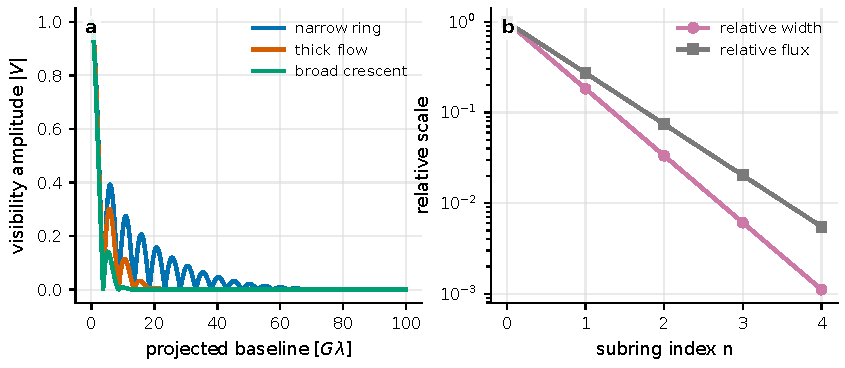
\includegraphics[width=0.94\linewidth]{figures/generated/chapter_12/ch12_photon_ring_visibility.pdf}
\caption{环状结构在长基线可见度中产生振荡。左图比较同样 \(42\,\mu{\rm as}\) 直径下不同厚度的环，窄环在更长基线上仍保留振荡；右图示意 photon subring 的宽度和通量随环绕次数下降，高阶子环通量小，但在足够长的基线可留下普适结构。}
\label{fig:chapter-12-photon-ring}
\end{figure}

EHT 图像中的亮环包含直接图像、一次透镜图像和高阶 photon subring，并不是数学上无限薄的 photon ring。吸积流厚度、光深、湍流和时间平均会把强引力的窄结构涂宽。Gralla 等强调，高阶 photon ring 在总通量中常很小；Johnson 等指出，足够长基线会解析掉宽的吸积流，只留下窄子环的普适振荡。可以把第 \(n\) 个子环的宽度和通量写成标度形式
\begin{equation}
  w_n\simeq w_0 e^{-\gamma n},\qquad
  F_n\simeq F_0 e^{-\beta n},
  \label{eq:ch12-20}
\end{equation}
\begin{formulaexplain}
\(w_n\) 和 \(F_n\) 是第 \(n\) 个 photon subring 的宽度和通量。指数标度描述多圈光路逐层变窄、变暗的强引力结构。
\end{formulaexplain}
其中 \(\gamma\) 与 photon orbit 的 Lyapunov 指数有关，\(\beta\) 还取决于发射和吸收。这个标度刻画强引力多圈光路的指数嵌套角结构；实际观测还要接上发射、吸收和时间平均模型 \citep{2019PhRvD.100b4018G,2020PhRvD.102l4004G,2013ApJ...777..170J}。

\Needspace{12\baselineskip}
多路径还意味着时间结构。若第 \(n\) 圈和第 \(n+1\) 圈光路的平均延迟差近似为 photon orbit 周期 \(T_\gamma\)，则相关函数中可能出现
\begin{equation}
  C(\tau)=\langle \delta I(t)\delta I(t+\tau)\rangle
  \quad\hbox{在}\quad
  \tau\simeq mT_\gamma
  \label{eq:ch12-21}
\end{equation}
\begin{formulaexplain}
\(C(\tau)\) 是强度自相关，\(T_\gamma\) 是 photon orbit 周期，\(m\) 是整数。若多路径贡献可见，相关函数可能在这些延迟附近出现弱峰。
\end{formulaexplain}
附近的弱峰。对 Sgr A*，\(T_\gamma\) 是分钟量级，和吸积流本身的 flare 时间重叠；对 M87*，它是天量级，源更稳定但观测调度更难。要把这类峰解释成强引力多路径，需要同时排除喷流 shock、盘湍流、散射屏、采样窗口和校准误差。偏振版本还可比较 \(Q,U,V\) 的延迟结构，EHT 对 M87* 和 Sgr A* 的偏振成像已经展示了这种信息的价值 \citep{2020PhRvD.101h4020H,2021PhRvD.104d4049G,2022PhRvD.106d3021C}。

\section{Hawking 温度为什么不是近期观测主线}

前几节讨论的是普通辐射如何被黑洞附近的强引力、等离子体和磁场组织。真正属于黑洞本身的量子辐射要从一个完全不同的数量级开始：Hawking 温度为
\begin{equation}
  T_H=\frac{\hbar c^3}{8\pi G M k_B}
  \simeq 6.17\times10^{-8}\,{\rm K}
  \left(\frac{M_\odot}{M}\right).
  \label{eq:ch12-22}
\end{equation}
\begin{formulaexplain}
\(T_H\) 是 Hawking 温度，和黑洞质量 \(M\) 成反比。天体质量黑洞温度极低，所以不会成为近期普通望远镜观测主线。
\end{formulaexplain}
恒星质量黑洞的 \(T_H\) 已经远低于 \(2.725\,\mathrm{K}\) 的 CMB；Sgr A* 和 M87* 更低到 \(10^{-14}-10^{-17}\,\mathrm{K}\)。蒸发时间近似为
\begin{equation}
  t_{\rm evap}\simeq
  2.1\times10^{67}\,{\rm yr}
  \left(\frac{M}{M_\odot}\right)^3 .
  \label{eq:ch12-23}
\end{equation}
\begin{formulaexplain}
\(t_{\rm evap}\) 是 Hawking 蒸发时间，随 \(M^3\) 增长。恒星质量和超大质量黑洞的蒸发时间远超宇宙年龄。
\end{formulaexplain}
普通天体黑洞的 Hawking 辐射远低于可预见望远镜灵敏度。只有假设很轻的原初黑洞，温度才会上升到高能波段；这类约束属于宇宙学和高能瞬变。对恒星质量和超大质量黑洞，近期观测主线仍是吸积流、偏振、可见度和 photon ring \citep{1974Natur.248...30H,1975CMaPh..43..199H}。

\begin{figure}[tbp]
\centering
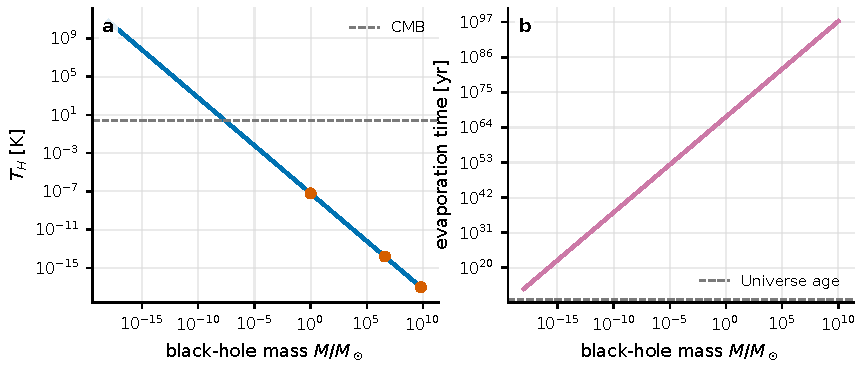
\includegraphics[width=0.94\linewidth]{figures/generated/chapter_12/ch12_hawking_temperature_scale.pdf}
\caption{Hawking 温度随质量反比下降，蒸发时间随质量三次方增加。恒星质量和超大质量黑洞的温度远低于 CMB，蒸发时间远超宇宙年龄；近期可操作的黑洞观测主要来自吸积流、偏振、可见度和时间结构。}
\label{fig:chapter-12-hawking}
\end{figure}


\chapter{爆发、瞬变和多信使量子天文学}
\label{chap:13}

\begin{chapteropening}
瞬变源把天体物理过程压缩到一个可观测的时间轴上。新星和超新星给出膨胀速度、距离和角尺度的联立问题；GRB 余辉追踪相对论激波、同步辐射和喷流角；千新星同时牵涉引力波定位、伽马射线延迟、颜色演化和 \(r\)-process ejecta；TDE 则从黑洞质量、回落率和再处理光球进入观测。平均光变曲线不够用；带有时间、频率、偏振、空间通道和触发来源的事件表才能同时约束触发时刻、背景、膨胀几何、颜色演化和多信使延迟 \citep{2014Natur.514..339C,2014Sci...345..554A,2008Sci...321..223S,1998ApJ...497L..17S,2004RvMP...76.1143P,2017PhRvL.119p1101A,2017ApJ...848L..12A,2017Natur.551...75S,2021ARA&A..59...21G}。
\end{chapteropening}

\section{为什么瞬变从触发似然开始}

一次瞬变观测从触发开始，但触发本身已经是一个统计推断。对第 \(k\) 个探测通道，事件率可以写成
\begin{equation}
  \lambda_k(t)=b_k(t)+A_{{\rm eff},k}(t)
  \int R_k(\nu,p,t)\,F_\nu(t,p)\,d\nu ,
  \label{eq:ch13-rate-response}
\end{equation}
\begin{formulaexplain}
\(\lambda_k(t)\) 是第 \(k\) 个通道的事件率，\(b_k\) 是背景，\(A_{\rm eff}\) 和 \(R_k\) 描述仪器响应，\(F_\nu\) 是源通量。触发从模型事件率开始。
\end{formulaexplain}
其中 \(\lambda_k\) 的单位是 \(\mathrm{s^{-1}}\)，\(b_k\) 是天光、宿主星系、暗计数和误触发贡献的背景率，\(A_{{\rm eff},k}\) 是有效面积，\(R_k\) 是包含带宽、量子效率、偏振选择和时间响应的仪器响应，\(F_\nu(t,p)\) 是源在频率 \(\nu\) 和偏振态 \(p\) 上的光子通量。光学瞬变的单通道事件率可以从低于 \(1\,\mathrm{s^{-1}}\) 到 \(10^6\,\mathrm{s^{-1}}\)；高能探测器常以较粗能道记录事件，射电和光学快探测器则更强调亚微秒到纳秒时间戳。

如果只关心一个快升慢降的触发窗口，常用的第一模型是
\begin{equation}
  \lambda(t)=b+A\exp\!\left[-\frac{t-t_0}{\tau}\right]H(t-t_0),
  \label{eq:ch13-exponential-rate}
\end{equation}
\begin{formulaexplain}
\(\lambda(t)\) 是快升慢降的事件率模型，\(b\) 是背景，\(A\) 是初始超额率，\(t_0\) 是起始时刻，\(\tau\) 是衰减时间。\(H\) 保证触发前没有该源项。
\end{formulaexplain}
\(b\) 是背景率，\(A\) 是触发后源的初始超额率，\(t_0\) 是物理起始时刻，\(\tau\) 是衰减时标，\(H\) 是阶跃函数。这里的 \(t\) 可用秒、小时或天，只要 \(A\) 和 \(b\) 用同一时间单位的倒数。GRB prompt emission 的 \(\tau\) 可以是 \(10^{-2}-10^2\,\mathrm{s}\)，光学 afterglow 的有效衰减时间通常是小时到天，新星和 TDE 的 \(\tau\) 可以到数十天或数百天。

事件表 \(\{t_j\}\) 对非齐次 Poisson 过程的对数似然为
\begin{equation}
  \ln L=\sum_{j=1}^{N}\ln \lambda(t_j)-\int_{t_{\rm min}}^{t_{\rm max}}\lambda(t)\,dt .
  \label{eq:ch13-poisson-likelihood}
\end{equation}
\begin{formulaexplain}
\(\ln L\) 是非齐次 Poisson 事件表似然。第一项奖励模型在真实光子时刻给出高事件率，第二项惩罚模型在整个窗口里预言过多计数。
\end{formulaexplain}
第一项在真实光子到达时刻评价模型事件率，第二项扣除模型在整个观测窗口内预言的总计数。式中的 \(\ln L\) 可由未分箱事件直接计算；如果把数据先分成很宽的时间 bin，\(t_0\) 和快速上升段的信息会被平均掉。这个形式也适用于带能量、频率和偏振标签的事件，只需把 \(\lambda(t)\) 换成 \(\lambda(t,\nu,p)\)，并把积分扩展到对应坐标。

\begin{figure}[tbp]
\centering
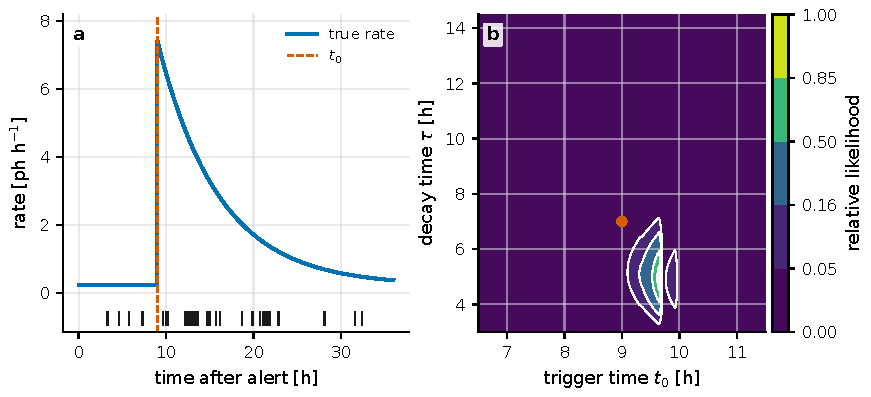
\includegraphics[width=0.92\linewidth]{figures/generated/chapter_13/ch13_transient_event_likelihood.pdf}
\caption{非齐次 Poisson 事件表怎样约束触发时间和衰减时间。左图中的竖线是单个光子到达时刻，蓝线是事件率模型；右图把同一事件表写成 \(t_0\) 和 \(\tau\) 的相对似然面。少量早期光子会强烈限制 \(t_0\)，而晚期背景决定 \(\tau\) 是否被高估。}
\label{fig:chapter-13-event-likelihood}
\end{figure}

触发器通常比较瞬变模型 \(M_{\rm tr}\) 和背景模型 \(M_{\rm bg}\)。用 odds ratio 写成
\begin{equation}
  {\cal O}_{\rm tr,bg}
  =
  \frac{P(M_{\rm tr})}{P(M_{\rm bg})}
  \frac{L(D|M_{\rm tr})}{L(D|M_{\rm bg})},
  \label{eq:ch13-trigger-odds}
\end{equation}
\begin{formulaexplain}
\({\cal O}_{\rm tr,bg}\) 是瞬变模型相对背景模型的 odds ratio。它把先验发生率和数据似然同时放进触发判断。
\end{formulaexplain}
\(D\) 是事件表或图像差分数据，\(P(M)\) 是先验发生率。若背景在窗口 \(\Delta t\) 内的期望计数为 \(\mu_b=b\Delta t\)，单窗口 Poisson false alarm probability 为
\begin{equation}
  P_{\rm FA}(N\ge n)=
  \sum_{m=n}^{\infty}\frac{\mu_b^m e^{-\mu_b}}{m!}.
  \label{eq:ch13-false-alarm}
\end{equation}
\begin{formulaexplain}
\(P_{\rm FA}\) 是背景单独产生 \(n\) 个或更多计数的误触发概率，\(\mu_b\) 是背景期望计数。触发阈值本质上是在控制这个尾概率。
\end{formulaexplain}
实际巡天还要乘以试验次数：时间窗口数、天空像素数、能道数和模板数都会增加误触发。FRB 搜索、伽马射线触发和光学差分巡天都面对同一问题，只是 \(\Delta t\) 从毫秒到天不等，背景从仪器噪声到变量源污染不等 \citep{2013Sci...341...53T,2017ApJ...835...29Y,2020Natur.587...59B,2020Natur.587...54C,2020Natur.581..391M}。

\section{膨胀源怎样把速度、时间和角尺度连起来}

新星和超新星的共同物理图像是一个速度分层的 ejecta。早期光球由光学厚的外层决定；随后谱线形成区向内退，低光学深度的壳层逐渐显露。若膨胀近似 homologous，即半径和速度满足 \(r=v(t-t_0)\)，角半径为
\begin{equation}
  \theta(t)=\frac{v_{\rm exp}(t-t_0)}{D}
  =
  5.8\,{\rm mas}
  \left(\frac{v_{\rm exp}}{10^8\,{\rm cm\,s^{-1}}}\right)
  \left(\frac{t-t_0}{10\,{\rm d}}\right)
  \left(\frac{D}{1\,{\rm kpc}}\right)^{-1}.
  \label{eq:ch13-angular-expansion}
\end{equation}
\begin{formulaexplain}
\(\theta(t)\) 是膨胀源角半径，\(v_{\rm exp}\) 是膨胀速度，\(D\) 是距离。它把谱线速度、爆发时间和角尺度连成几何距离问题。
\end{formulaexplain}
\(\theta\) 可由成像、干涉或模型可见度估计；\(v_{\rm exp}\) 常由谱线的 Doppler 宽度或吸收最低点估计；\(D\) 是距离。新星在 \(D\sim1-5\,\mathrm{kpc}\)、\(v_{\rm exp}\sim10^8\,\mathrm{cm\,s^{-1}}\) 时，几天到几十天内可达到毫角秒尺度。Type Ia 超新星在 \(D\sim10-100\,\mathrm{Mpc}\)、\(v_{\rm exp}\sim10^9\,\mathrm{cm\,s^{-1}}\) 时，十天角半径只有数微角秒。GW170817 类千新星速度可达 \(0.1-0.3c\)，但距离约 \(40\,\mathrm{Mpc}\)，早期角尺度仍在微角秒以下。

\begin{figure}[tbp]
\centering
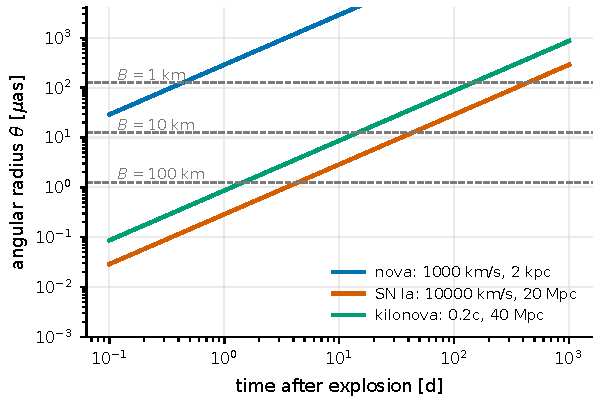
\includegraphics[width=0.92\linewidth]{figures/generated/chapter_13/ch13_expanding_fireball_resolution.pdf}
\caption{膨胀源的角半径由速度、时间和距离共同决定。银河系新星虽然速度低，但距离近，角尺度最快进入毫角秒范围；低红移 Type Ia 超新星和千新星速度更高，却因距离远落在微角秒范围。水平虚线给出 \(\lambda=0.5\,\mu{\rm m}\) 时不同光学基线的 \(\lambda/B\) 标度。}
\label{fig:chapter-13-expansion}
\end{figure}

谱线把速度投影到波长上：
\begin{equation}
  v_{\rm los}\simeq c\,\frac{\lambda_{\rm obs}-\lambda_0}{\lambda_0},
  \label{eq:ch13-doppler-line}
\end{equation}
\begin{formulaexplain}
\(v_{\rm los}\) 是视向速度，\(\lambda_{\rm obs}\) 和 \(\lambda_0\) 是观测与实验室波长。谱线位移把 ejecta 的速度层投影到波长轴上。
\end{formulaexplain}
\(\lambda_0\) 是实验室波长，\(\lambda_{\rm obs}\) 是观测波长。P-Cygni absorption 的蓝端常近似代表外层最快物质，吸收最低点更接近光学深度最大的速度层；发射线半宽则混合了几何、光学深度和密度分布。若每个谱线通道都能测角尺度或相关函数，数据会变成一组 \(\theta(v_{\rm los})\)，可以区分球壳、双锥、赤道环和 polar wind。

强度干涉中，一个圆对称均匀光盘的二阶相关给出 \(|V|^2\)。对应的一阶可见度模长为
\begin{equation}
  |V(B)|=
  \left|
  \frac{2J_1(\pi B\Theta/\lambda)}{\pi B\Theta/\lambda}
  \right|,
  \label{eq:ch13-uniform-disk-visibility}
\end{equation}
\begin{formulaexplain}
\(|V(B)|\) 是均匀圆盘可见度模长，\(\Theta\) 是角直径，\(B\) 是基线，\(\lambda\) 是波长。强度干涉测 \(|V|^2\)，可反推瞬变源角尺度。
\end{formulaexplain}
\(\Theta=2\theta\) 是角直径，\(B\) 是投影基线，\(\lambda\) 是观测波长。这个公式假设圆对称、单波长和无强 limb darkening；真实新星和超新星更常需要薄壳、环、椭球或多组分模型。把角膨胀和谱线速度合并，可以得到 expansion parallax：
\begin{equation}
  D=\frac{v_{\rm exp}(t-t_0)}{\theta(t)}.
  \label{eq:ch13-expansion-parallax}
\end{equation}
\begin{formulaexplain}
\(D\) 是膨胀视差距离。只有当 \(v_{\rm exp}\) 和 \(\theta(t)\) 对应同一物质层时，这个几何距离才不会被速度分层系统偏置。
\end{formulaexplain}
左边的 \(D\) 是几何距离，右边的 \(v_{\rm exp}\) 应和 \(\theta\) 对应同一层物质。若谱线测到的是外层高速吸收，而角尺度来自连续谱光球，距离会系统偏差。

经典新星是白矮星表面的热核爆发，典型 ejecta mass 为 \(10^{-5}-10^{-4}M_\odot\)，速度超过 \(10^3\,\mathrm{km\,s^{-1}}\)。Fermi 发现新星是 GeV \(\gamma\)-ray 源之后，物理图像转向双流结构：慢而密的 equatorial ejecta 被双星轨道塑形，快的 polar wind 撞上它，在内部激波中加速粒子。V959 Mon 的 \(\gamma\)-ray 发射持续约 \(12\,\mathrm{d}\)，高分辨射电成像显示 shock 位于 polar flow 和 equatorial material 的交界，热 ejecta mass 约 \(4\times10^{-5}M_\odot\) \citep{2014Natur.514..339C,2014Sci...345..554A}。在这种源里，\(v_{\rm exp}\) 包含 equatorial 和 polar 两个速度组分；谱线、射电图像和光子事件表要共同拟合。

Type Ia 超新星通常先由亮度校正进入距离问题。Phillips relation 用 \(B\) band 衰减率 \(\Delta m_{15}(B)\) 校正峰值绝对星等；宇宙学应用再把校正后的距离模数写成
\begin{equation}
  \mu = m_B - M_B + \alpha x_1-\beta C+\Delta_{\rm host},
  \label{eq:ch13-snia-distance-modulus}
\end{equation}
\begin{formulaexplain}
\(\mu\) 是距离模数，\(m_B\) 和 \(M_B\) 是观测与标准化峰值星等，\(x_1\) 是光变宽度，\(C\) 是颜色。Type Ia 标准化本质上是在修正光度。
\end{formulaexplain}
\(m_B\) 是观测峰值星等，\(M_B\) 是标准化绝对星等，\(x_1\) 或类似参数描述光变曲线宽度，\(C\) 是颜色，\(\alpha\)、\(\beta\) 和 \(\Delta_{\rm host}\) 由样本拟合。近邻样本中 \(m_B\sim10-16\) 的 Type Ia 可以在小望远镜上得到高信噪光变曲线；宇宙学样本常在 \(m_B\sim22-25\)。如果同时测到角膨胀，就可以用几何距离交叉检查光度距离。这个目标很难，因为十几天的 Type Ia 角直径只有微角秒量级；在长基线光学强度干涉中，它属于难度很高但科学收益明确的瞬变应用 \citep{1993ApJ...413L.105P,1998AJ....116.1009R,1999ApJ...517..565P}。

Type Ia 的偏振告诉我们 ejecta 是否真的近似球对称。Stokes 参数常写为
\begin{equation}
  q=\frac{Q}{I},\qquad
  u=\frac{U}{I},\qquad
  P=\sqrt{q^2+u^2},
  \label{eq:ch13-stokes-polarization}
\end{equation}
\begin{formulaexplain}
\(q,u\) 是归一化 Stokes 参数，\(P\) 是线偏振度。偏振把 ejecta 非球对称和散射几何写进可观测量。
\end{formulaexplain}
\(q\)、\(u\) 和 \(P\) 是无量纲，通常用百分数报告。SN 1999by 在最大光附近有 \(P\simeq0.3-0.8\%\)，Si II \(6150\,\text{\AA}\) 附近有约 \(0.4\%\) 的偏振变化，模型指向约 \(20\%\) 的整体非球对称，并且 Si 层和连续谱大体共享同一对称轴 \citep{2001ApJ...556..302H}。\(\Theta(t)\)、\(v_{\rm exp}\) 和 \(P(t,\lambda)\) 应放在同一个几何模型里解释：角尺度来自光球形状，谱线来自速度层，偏振来自散射几何。

核心坍缩超新星的最早窗口是 shock breakout。激波离表面还有一段距离时，辐射先扩散出来形成 radiative precursor。令 \(d\) 为激波到表面的深度，\(\rho\) 为局部密度，\(\kappa\) 为 opacity，光学深度 \(\tau\simeq\kappa\rho d\)。breakout 条件近似为
\begin{equation}
  t_{\rm diff}\simeq \frac{\tau d}{c}\simeq \frac{d}{v_s},
  \qquad
  \tau\simeq \frac{c}{v_s},
  \label{eq:ch13-shock-breakout-condition}
\end{equation}
\begin{formulaexplain}
\(t_{\rm diff}\) 是辐射扩散时间，\(d\) 是激波到表面的深度，\(v_s\) 是激波速度。breakout 发生在扩散时间赶上动力学时间时。
\end{formulaexplain}
\(v_s\) 是 shock velocity。对红超巨星，\(v_s\sim1-2\times10^9\,\mathrm{cm\,s^{-1}}\)，早期能量主要出现在 extreme UV 或 soft X-ray，光学发现常滞后数天。SNLS-04D2dc 的 GALEX UV 数据显示了 shock 到达表面前的 radiative precursor，并给出 envelope 结构和 progenitor radius 的约束 \citep{2008Sci...321..223S,2011ApJ...727..104C}。这些小时级早期信号要求触发系统压缩 alert、slew、acquisition 和第一轮曝光之间的延迟。

\section{千新星怎样把多信使延迟变成物理约束}

GW170817 给出了多信使瞬变的清楚时间轴。引力波给出 binary neutron star inspiral 的 coalescence time 和距离，Fermi/GBM 与 INTEGRAL 在约 \(1.74\pm0.05\,\mathrm{s}\) 后看到 GRB 170817A，光学 counterpart 在十几小时内被定位，随后 UV/optical/NIR 颜色从蓝快速转红 \citep{2017PhRvL.119p1101A,2017ApJ...848L..13A,2017ApJ...848L..12A,2017ApJ...848L..17C,2017Natur.551...75S,2017ApJ...848L..27T,2017ApJ...848L..24V,2017ApJ...848L..18N,2017Sci...358.1565E,2017ApJ...851L..21V}。

多信使延迟定义为
\begin{equation}
  \Delta t_{a-b}=t_a-t_b .
  \label{eq:ch13-mm-delay}
\end{equation}
\begin{formulaexplain}
\(\Delta t_{a-b}\) 是两个信使或波段的到达时间差。只有把所有时间戳放到同一时标系统中，多信使延迟才有物理意义。
\end{formulaexplain}
\(t_a\) 和 \(t_b\) 是同一时标系统中的到达时间。解释 \(\Delta t\) 时要分成三部分：
\begin{equation}
  \Delta t_{\rm obs}
  =
  \Delta t_{\rm engine}
  +
  \Delta t_{\rm prop}
  +
  \Delta t_{\rm clock}.
  \label{eq:ch13-delay-budget}
\end{equation}
\begin{formulaexplain}
\(\Delta t_{\rm obs}\) 是观测延迟，分成源内发射延迟、传播延迟和时钟/处理误差。这个分解避免把源物理误认为基本传播效应。
\end{formulaexplain}
\(\Delta t_{\rm engine}\) 是源内发射延迟，例如 merger 到 jet breakout 的时间；\(\Delta t_{\rm prop}\) 是传播延迟，可用于约束传播速度差或等效质量；\(\Delta t_{\rm clock}\) 是仪器时钟和数据处理误差。若源距 \(D\) 已知，传播速度差的数量级为
\begin{equation}
  \frac{|\Delta v|}{c}
  \lesssim
  \frac{|\Delta t_{\rm prop}|}{D/c}
  =
  2.4\times10^{-16}
  \left(\frac{\Delta t_{\rm prop}}{1\,{\rm s}}\right)
  \left(\frac{D}{40\,{\rm Mpc}}\right)^{-1}.
  \label{eq:ch13-speed-difference}
\end{equation}
\begin{formulaexplain}
\(|\Delta v|/c\) 是传播速度差的相对量级，\(D/c\) 是光行时。远距离让秒级传播延迟对应极小的速度差约束。
\end{formulaexplain}
这个公式左边不能直接把 \(1.74\,\mathrm{s}\) 全部当作传播延迟，因为 GRB 发射本身可能晚于 merger。它的用处是把“可容许的新传播效应”放到正确数量级上。

\begin{figure}[tbp]
\centering
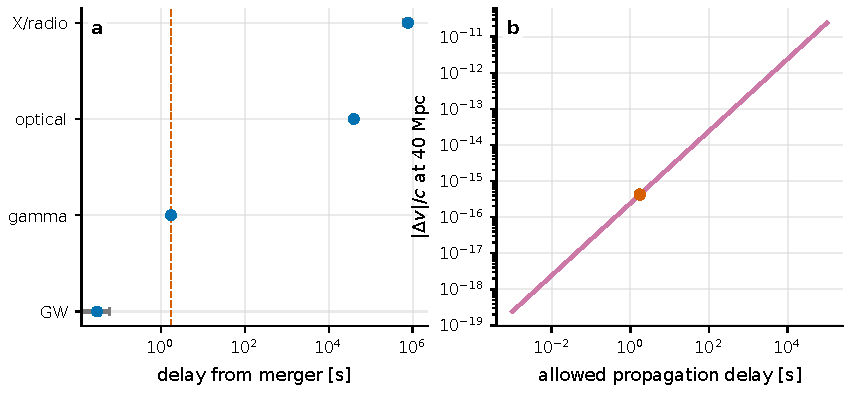
\includegraphics[width=0.92\linewidth]{figures/generated/chapter_13/ch13_multimessenger_delay.pdf}
\caption{多信使延迟的两个读法。左图比较 merger 后不同通道的到达时间：GW 和 \(\gamma\)-ray 位于秒尺度，光学 counterpart 通常受定位和昼夜周期限制，X-ray/radio 可在天到月尺度出现。右图把传播延迟换算成 \(40\,\mathrm{Mpc}\) 距离上的 \(|\Delta v|/c\) 数量级；源内发射延迟越不确定，传播约束越保守。}
\label{fig:chapter-13-mm-delay}
\end{figure}

千新星的光度来自 neutron-rich ejecta 中 \(r\)-process 放射性衰变热化。一个常用标度是
\begin{equation}
  \dot q(t)\simeq
  2\times10^{10}
  \left(\frac{t}{1\,{\rm d}}\right)^{-1.3}
  {\rm erg\,s^{-1}\,g^{-1}},
  \label{eq:ch13-rprocess-heating}
\end{equation}
\begin{formulaexplain}
\(\dot q(t)\) 是 \(r\)-process 物质单位质量加热率。千新星光度的能量源来自这项放射性衰变热化。
\end{formulaexplain}
\(\dot q\) 是单位质量加热率。进入光度的是 \(\epsilon_{\rm th}M_{\rm ej}\dot q\)，其中 \(\epsilon_{\rm th}<1\) 是热化效率，\(M_{\rm ej}\) 是 ejecta mass。扩散时间决定光变峰值：
\begin{equation}
  t_{\rm pk}\simeq
  \left(\frac{\kappa M_{\rm ej}}{4\pi v_{\rm ej}c}\right)^{1/2}
  =
  0.6\,{\rm d}
  \left(\frac{\kappa}{0.5\,{\rm cm^2\,g^{-1}}}\right)^{1/2}
  \left(\frac{M_{\rm ej}}{0.01M_\odot}\right)^{1/2}
  \left(\frac{v_{\rm ej}}{0.3c}\right)^{-1/2}.
  \label{eq:ch13-kilonova-diffusion}
\end{equation}
\begin{formulaexplain}
\(t_{\rm pk}\) 是千新星峰值时间，\(\kappa\) 是 opacity，\(M_{\rm ej}\) 是抛射质量，\(v_{\rm ej}\) 是速度。高 opacity 或大质量会让峰值更晚更红。
\end{formulaexplain}
\(\kappa\) 是 opacity。lanthanide-poor ejecta 的 \(\kappa\sim0.3-1\,\mathrm{cm^2\,g^{-1}}\)，峰值在一天左右且颜色较蓝；lanthanide-rich ejecta 的 \(\kappa\sim5-30\,\mathrm{cm^2\,g^{-1}}\)，峰值可推到数天到十天并转向 NIR。

早期光谱能用黑体半径和温度近似：
\begin{equation}
  L_{\rm bol}=4\pi R_{\rm BB}^2\sigma_{\rm SB}T_{\rm BB}^4 .
  \label{eq:ch13-kilonova-blackbody}
\end{equation}
\begin{formulaexplain}
\(L_{\rm bol}\) 是总辐射光度，\(R_{\rm BB}\) 和 \(T_{\rm BB}\) 是黑体半径和温度。早期 SED 拟合可把颜色演化转成膨胀速度和发光面积。
\end{formulaexplain}
GW170817 在约 \(0.6\,\mathrm{d}\) 时可用 \(T_{\rm BB}\simeq8300\,\mathrm{K}\)、\(R_{\rm BB}\simeq4.5\times10^{14}\,\mathrm{cm}\)、\(L_{\rm bol}\simeq5\times10^{41}\,\mathrm{erg\,s^{-1}}\) 描述，对应 \(v\simeq0.3c\)。随后的 SED 迅速偏离单一黑体，UV/blue flux 衰减，NIR 相对增强。两组分模型通常需要 \(M_{\rm ej,blue}\sim0.01M_\odot\)、\(v_{\rm blue}\sim0.27-0.3c\)，再加 \(M_{\rm ej,red}\sim0.04M_\odot\)、\(v_{\rm red}\sim0.1c\) 的红组分；三组分模型会把中间 opacity 的 purple component 单独列出 \citep{2017Natur.551...75S,2017ApJ...848L..17C,2017ApJ...848L..27T,2017Sci...358.1565E}。

\begin{figure}[tbp]
\centering
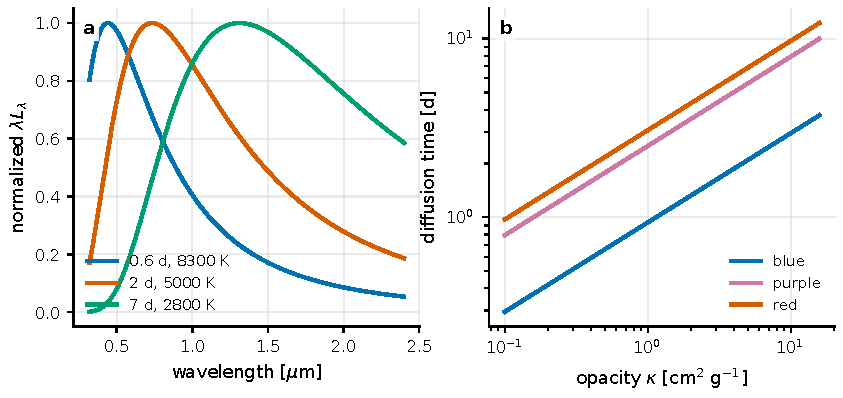
\includegraphics[width=0.92\linewidth]{figures/generated/chapter_13/ch13_kilonova_color_evolution.pdf}
\caption{千新星从蓝到红的演化。左图用三个黑体 SED 标示温度降低后峰值波长向红外移动；右图用扩散时间公式显示 opacity 越大、质量越大、速度越低，峰值越晚。GW170817 的蓝组分快而低 opacity，红组分慢而高 opacity，因此单一 ejecta 组分无法同时解释早期蓝光和晚期 NIR。}
\label{fig:chapter-13-kilonova}
\end{figure}

引力波还给出标准警报器距离。低红移下可粗略写成
\begin{equation}
  H_0\simeq \frac{cz_{\rm host}}{D_L},
  \label{eq:ch13-standard-siren}
\end{equation}
\begin{formulaexplain}
\(H_0\) 是 Hubble 常数，\(z_{\rm host}\) 是宿主红移，\(D_L\) 是引力波给出的光度距离。标准警报器用距离和红移直接测宇宙膨胀率。
\end{formulaexplain}
\(z_{\rm host}\) 是宿主星系红移，\(D_L\) 是从引力波振幅推断的 luminosity distance。GW170817 的主要退化来自 inclination 和 distance：面对面的 binary 既更亮也更难确定倾角。电磁 counterpart 提供宿主、红移、喷流视角和 ejecta 几何，从而减少一部分退化。多信使分析把同一物理事件的这些投影放进一个联合似然。

\section{GRB 余辉怎样把喷流几何写进光变}

GRB prompt emission 给出高能触发，afterglow 给出外激波的可追踪物理。一个相对论 shell 撞入外部介质后，观测时刻 \(t\) 与半径 \(R\) 和 Lorentz factor \(\Gamma\) 的关系近似为
\begin{equation}
  t\simeq \frac{(1+z)R}{4\Gamma^2c}.
  \label{eq:ch13-grb-arrival-time}
\end{equation}
\begin{formulaexplain}
\(t\) 是观测到达时刻，\(R\) 是激波半径，\(\Gamma\) 是 Lorentz 因子。相对论 beaming 让大半径外激波被压缩到很短观测时间。
\end{formulaexplain}
同样的半径，因为 relativistic beaming 和 light-travel-time effect，会被压缩到更短的观测时间。典型 early afterglow 有 \(\Gamma\sim10-300\)，\(R\sim10^{16}-10^{18}\,\mathrm{cm}\)，光学可在触发后几十秒到几分钟进入望远镜视场 \citep{1997ApJ...476..232M,1998ApJ...497L..17S,1998Natur.395..670G,1999PhR...314..575P,2004RvMP...76.1143P,2006ARA&A..44..507W}。

若电子能谱为
\begin{equation}
  N(\gamma_e)\,d\gamma_e \propto \gamma_e^{-p}\,d\gamma_e,
  \qquad \gamma_e>\gamma_m,
  \label{eq:ch13-electron-powerlaw}
\end{equation}
\begin{formulaexplain}
\(N(\gamma_e)\) 是电子 Lorentz 因子分布，\(p\) 是能谱指数，\(\gamma_m\) 是低能截止。同步余辉谱斜率主要由 \(p\) 控制。
\end{formulaexplain}
同步辐射谱在 \(\nu_m\) 和 \(\nu_c\) 附近出现 break。常用观测形式为
\begin{equation}
  F_\nu(t)\propto t^{-\alpha}\nu^{-\beta}.
  \label{eq:ch13-afterglow-powerlaw}
\end{equation}
\begin{formulaexplain}
\(F_\nu(t)\) 是余辉通量密度，\(\alpha\) 是时间衰减指数，\(\beta\) 是谱指数。观测通常先把光变和颜色压缩成这两个斜率。
\end{formulaexplain}
在均匀介质、adiabatic、slow-cooling 且 \(\nu_m<\nu<\nu_c\) 的区间，
\begin{equation}
  \beta=\frac{p-1}{2},
  \qquad
  \alpha=\frac{3(p-1)}{4}.
  \label{eq:ch13-closure-relation}
\end{equation}
\begin{formulaexplain}
closure relation 把观测斜率 \(\alpha,\beta\) 和电子指数 \(p\) 联系起来。若数据偏离它，说明介质、冷却区间或能量注入假设可能不成立。
\end{formulaexplain}
若 \(p=2.2\)，则 \(\beta\simeq0.6\)、\(\alpha\simeq0.9\)。在 \(\nu>\nu_c\) 时常变为 \(\alpha=(3p-2)/4\)。这些 closure relations 的假设很明确：外部介质简单、能量注入不强、microphysical parameters 不剧烈演化、观测频段没有跨过 break。观测上，光学 afterglow 在爆发后一天常为 \(19-20\) mag；偏振可达百分之几到约 \(10\%\)，与同步辐射和喷流几何有关 \citep{2004RvMP...76.1143P,2006ARA&A..44..507W}。

\begin{figure}[tbp]
\centering
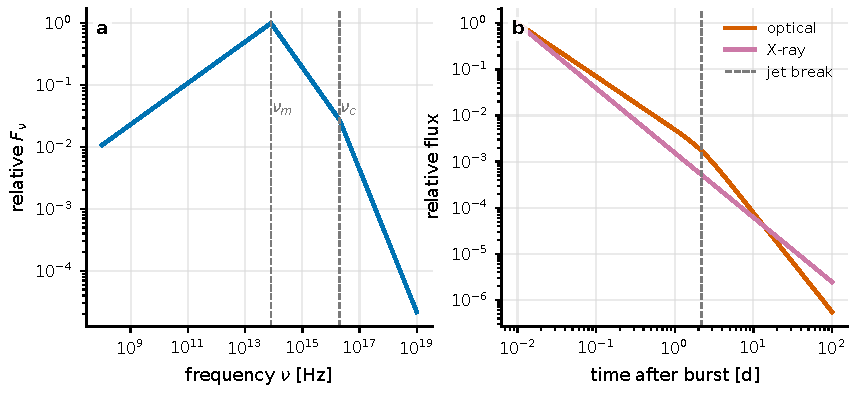
\includegraphics[width=0.92\linewidth]{figures/generated/chapter_13/ch13_afterglow_synchrotron_breaks.pdf}
\caption{GRB afterglow 的同步辐射读法。左图显示 \(\nu_m\) 和 \(\nu_c\) 把谱分成不同斜率区间；右图显示喷流 break 前后光变曲线变陡。若光学和 X-ray 不在同一谱段，它们的 \(\alpha\) 和 \(\beta\) 不必相同，需要先判断观测频率相对 \(\nu_m\)、\(\nu_c\) 的位置。}
\label{fig:chapter-13-afterglow}
\end{figure}

当 \(\Gamma\) 降到约 \(1/\theta_j\) 时，观测者开始看到喷流边缘，光变曲线出现 achromatic jet break。常用估算为
\begin{equation}
  \theta_j\simeq
  0.10
  \left(\frac{t_j}{1\,{\rm d}}\right)^{3/8}
  \left(\frac{1+z}{2}\right)^{-3/8}
  \left(\frac{E_{\rm iso,52}}{n_0}\right)^{-1/8},
  \label{eq:ch13-jet-opening-angle}
\end{equation}
\begin{formulaexplain}
\(\theta_j\) 是喷流半张角，\(t_j\) 是 jet break 时间，\(E_{\rm iso}\) 和 \(n_0\) 是各向同性能量和外部密度。break 越晚，喷流通常越宽。
\end{formulaexplain}
\(\theta_j\) 以 rad 为单位，\(t_j\) 是 break time，\(E_{\rm iso,52}=E_{\rm iso}/10^{52}\,\mathrm{erg}\)，\(n_0\) 是外部介质数密度的 \(\mathrm{cm^{-3}}\) 数值。系数随模型细节而变，但弱指数控制了误差传播：即使 \(E_{\rm iso}\) 或 \(n\) 不确定一个数量级，\(\theta_j\) 也只变几十个百分点。主要风险来自误分类：chromatic break、能量注入、密度跳变或 supernova bump 都可能被误判为 jet break \citep{2003Natur.423..847H,2004ApJ...611.1005G}。

GRB 980425/SN 1998bw 和 GRB 030329/SN 2003dh 把长 GRB 与 broad-lined Type Ic 超新星联系起来；短 GRB 与 BNS merger 的联系在 GW170817 后变成了直接多信使事实。GRB 要求望远镜系统处理极端时间层级：秒级高能触发、分钟级光学 flash、小时到天的 afterglow、周到月的 radio calorimetry，以及可能叠加的 supernova 或 kilonova。事件表除了 flux，还要保留每个阶段的时间基准和频段连接。

\section{TDE 怎样从回落率和再处理光球读出黑洞质量}

潮汐瓦解事件发生在恒星靠近超大质量黑洞时。潮汐半径为
\begin{equation}
  r_t\simeq R_\ast\left(\frac{M_\bullet}{M_\ast}\right)^{1/3},
  \label{eq:ch13-tidal-radius}
\end{equation}
\begin{formulaexplain}
\(r_t\) 是潮汐半径，\(M_\bullet\) 是黑洞质量，\(M_\ast,R_\ast\) 是恒星质量和半径。恒星进入这个半径内会被黑洞潮汐力撕裂。
\end{formulaexplain}
\(M_\bullet\) 是黑洞质量，\(M_\ast\) 和 \(R_\ast\) 是恒星质量和半径。Schwarzschild 半径为
\begin{equation}
  r_s=\frac{2GM_\bullet}{c^2}.
  \label{eq:ch13-schwarzschild-radius-tde}
\end{equation}
\begin{formulaexplain}
\(r_s\) 是 Schwarzschild 半径。比较 \(r_t\) 和 \(r_s\) 可判断恒星是先被潮汐撕裂，还是在亮 flare 前直接落入黑洞。
\end{formulaexplain}
当 \(r_t\lesssim r_s\) 时，恒星可在产生明亮 flare 前被吞没；主序星 TDE 因而最常见于 \(M_\bullet\sim10^5-10^7M_\odot\)，到 \(10^8M_\odot\) 附近选择效应变强 \citep{1988Natur.333..523R,2021ARA&A..59...21G}。

最早返回的 bound debris 给出 fallback time：
\begin{equation}
  t_{\rm min}\simeq
  41\,{\rm d}
  \left(\frac{M_\bullet}{10^6M_\odot}\right)^{1/2}
  \left(\frac{M_\ast}{M_\odot}\right)^{-1}
  \left(\frac{R_\ast}{R_\odot}\right)^{3/2}.
  \label{eq:ch13-tde-fallback-time}
\end{equation}
\begin{formulaexplain}
\(t_{\rm min}\) 是最早 bound debris 返回近心点的时间。它随黑洞质量约按 \(M_\bullet^{1/2}\) 增长，是 TDE rise time 的重要标尺。
\end{formulaexplain}
理想情况下，晚期回落率为
\begin{equation}
  \dot M_{\rm fb}\simeq
  \frac{M_\ast}{3t_{\rm min}}
  \left(\frac{t}{t_{\rm min}}\right)^{-5/3}.
  \label{eq:ch13-tde-fallback-rate}
\end{equation}
\begin{formulaexplain}
\(\dot M_{\rm fb}\) 是 debris 回落率。理想 \(t^{-5/3}\) 衰减是 TDE 的经典标志，但观测光度还会受 circularization 和再处理影响。
\end{formulaexplain}
\(\dot M_{\rm fb}\) 的单位常用 \(M_\odot\,\mathrm{yr^{-1}}\)。Eddington accretion rate 为
\begin{equation}
  \dot M_{\rm Edd}
  =
  \frac{L_{\rm Edd}}{\eta c^2}
  \simeq
  0.022
  \left(\frac{M_\bullet}{10^6M_\odot}\right)
  \left(\frac{\eta}{0.1}\right)^{-1}
  M_\odot\,{\rm yr^{-1}} ,
  \label{eq:ch13-eddington-rate}
\end{equation}
\begin{formulaexplain}
\(\dot M_{\rm Edd}\) 是 Eddington 吸积率，\(\eta\) 是辐射效率。把 \(\dot M_{\rm fb}\) 和它比较，可判断回落是否进入超 Eddington 阶段。
\end{formulaexplain}
\(\eta\) 是辐射效率。对 \(10^6M_\odot\) 黑洞，太阳型恒星的 peak fallback 可以显著超 Eddington，但光学光度未必同样超 Eddington，因为 circularization、wind、obscuration 和 reprocessing 会把内盘能量重分配到 UV/optical。

\begin{figure}[tbp]
\centering
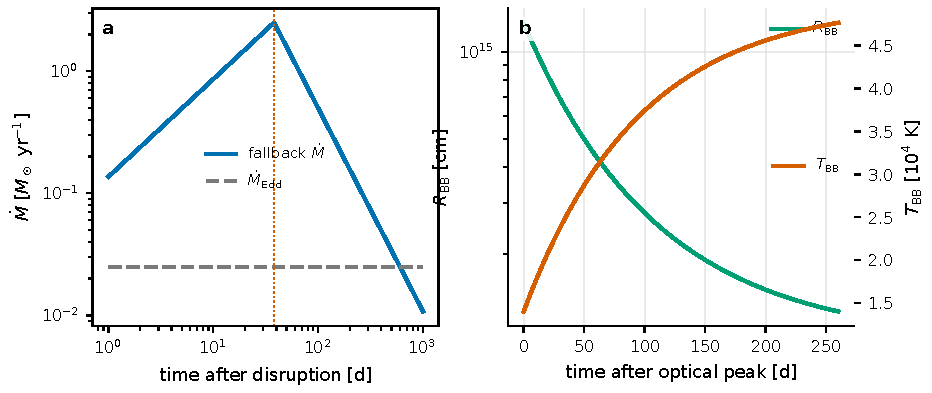
\includegraphics[width=0.92\linewidth]{figures/generated/chapter_13/ch13_tde_fallback_reprocessing.pdf}
\caption{TDE 的回落和再处理。左图显示 \(t^{-5/3}\) fallback 在几十天尺度进入衰减段，并可长期高于 \(10^6M_\odot\) 黑洞的 Eddington accretion rate。右图给出 optical/UV 黑体光球的一种典型演化：半径从 \(10^{15}\,\mathrm{cm}\) 量级收缩到 \(10^{14}\,\mathrm{cm}\)，温度从 \(10^4\,\mathrm{K}\) 量级升到数 \(10^4\,\mathrm{K}\)。}
\label{fig:chapter-13-tde}
\end{figure}

光学 TDE 的黑体半径通常为 \(10^{14}-10^{15}\,\mathrm{cm}\)，比 \(10^6M_\odot\) 黑洞的几倍 \(r_s\) 大得多；温度常为几 \(10^4\,\mathrm{K}\)，演化比普通超新星慢。AT2018zr 是 ZTF 早期样本中第一个有很好 rise-to-peak 覆盖的 TDE，最早 ZTF 检测约在峰值前 \(50\,\mathrm{d}\)。其光学/UV 黑体温度早期约 \(1.4\times10^4\,\mathrm{K}\)，晚期可升到 \(>5\times10^4\,\mathrm{K}\)，黑体半径从 \(10^{15.1}\,\mathrm{cm}\) 降到 \(<10^{14}\,\mathrm{cm}\)；X-ray luminosity 比同时期 optical/UV blackbody luminosity 低数个数量级，说明 obscuration 或 reprocessing 不能忽略 \citep{2019ApJ...872..198V,2021ARA&A..59...21G}。

喷流型 TDE 例如 Swift J1644+57 则把事件表推向高能和快速变率：X-ray 可强烈闪烁，radio emission 跟踪 outflow 与外部介质相互作用 \citep{2011Sci...333..203B}。IceCube-170922A 和 blazar 的多信使联系属于另一类源；TDE 中也有高能 neutrino 关联的候选个例 \citep{2021NatAs...5..510S}。在长时标瞬变里，事件表仍然要保留完整时间信息。判断一个高能事件是否属于 optical flare，需要同时看天球位置、时间延迟、能量、方向误差和源演化是否相容。

\section{机会目标观测怎样避免只抢快不算误差}

瞬变观测成败常由响应时间决定。一个实用条件是
\begin{equation}
  t_{\rm alert}+t_{\rm slew}+t_{\rm acq}+t_{\rm exp}
  < f_{\rm samp}\,t_{\rm evol},
  \label{eq:ch13-response-budget}
\end{equation}
\begin{formulaexplain}
左边是从触发到第一组有效曝光的总响应时间，右边是希望采样的源变化时间。机会目标观测要把“快”量化成这个预算。
\end{formulaexplain}
\(t_{\rm alert}\) 是触发发布延迟，\(t_{\rm slew}\) 是望远镜转向，\(t_{\rm acq}\) 是目标确认和导星，\(t_{\rm exp}\) 是第一组有效曝光，\(t_{\rm evol}\) 是源变化时标。若希望解析上升段，\(f_{\rm samp}\sim0.1\) 比较合理。GRB optical flash 的 \(t_{\rm evol}\) 可小于 \(10^3\,\mathrm{s}\)，GW counterpart 的蓝光阶段约一天，新星早期射电/光谱结构可在天到周内变化，TDE 的 rise time 则常为数十天。

普通成像曝光的信噪比为
\begin{equation}
  {\rm SNR}=
  \frac{N_s}
  {\left(N_s+N_b+n_{\rm pix}\sigma_{\rm read}^2\right)^{1/2}},
  \label{eq:ch13-imaging-snr}
\end{equation}
\begin{formulaexplain}
\({\rm SNR}\) 是成像信噪比，\(N_s\) 是源计数，\(N_b\) 是背景计数，读出噪声按像素数累加。曝光选择要同时看源、背景和读出噪声。
\end{formulaexplain}
\(N_s\) 是源计数，\(N_b\) 是背景计数，\(n_{\rm pix}\) 是 aperture 内像素数，\(\sigma_{\rm read}\) 是每像素读出噪声。强度干涉或 photon-pair 统计还要看 pair 数：
\begin{equation}
  N_{\rm pair}\simeq r_1 r_2\,\Delta t\,T,
  \qquad
  \delta C\simeq N_{\rm pair}^{-1/2},
  \label{eq:ch13-pair-statistics}
\end{equation}
\begin{formulaexplain}
\(N_{\rm pair}\) 是相关窗口内的光子对数，\(r_1,r_2\) 是事件率，\(\Delta t\) 是相关窗口，\(T\) 是累计时间。相关误差按光子对数平方根下降。
\end{formulaexplain}
\(r_1\) 和 \(r_2\) 是两台望远镜的事件率，\(\Delta t\) 是相关窗口，\(T\) 是累计时间。若 \(r_1=r_2=10^6\,\mathrm{s^{-1}}\)、\(\Delta t=100\,\mathrm{ps}\)、\(T=1\,\mathrm{h}\)，则 \(N_{\rm pair}\sim3.6\times10^5\)，纯 Poisson 相关误差约 \(1.7\times10^{-3}\)。这只是统计下限，真实误差还包括时间同步、dead time、光谱带宽、偏振泄漏和背景变化。

宿主关联也有明确的数量级。若瞬变位置误差半径为 \(r\)，深度 \(m\) 内背景星系面密度为 \(\Sigma(<m)\)，随机重合概率可写成
\begin{equation}
  P_{\rm cc}=1-\exp[-\pi r^2\Sigma(<m)].
  \label{eq:ch13-chance-coincidence}
\end{equation}
\begin{formulaexplain}
\(P_{\rm cc}\) 是随机宿主重合概率，\(r\) 是定位误差半径，\(\Sigma(<m)\) 是背景星系面密度。定位越差、星系越密，宿主关联越不可靠。
\end{formulaexplain}
GW170817 的 Virgo 加入把天空定位显著收缩到几十平方度量级，使光学巡天能够在同一夜定位宿主；TDE 选择则需要亚角秒 astrometry 来证明 flare 与星系核一致。AT2018zr 的 ZTF 分析显示，对核瞬变，多个差分检测可把 host-flare offset 的统计误差压到远小于单次 seeing 的尺度 \citep{2017PhRvL.119p1101A,2017ApJ...848L..12A,2019ApJ...872..198V}。

\begin{longtable}{@{}p{0.14\linewidth}p{0.19\linewidth}p{0.27\linewidth}p{0.28\linewidth}@{}}
\toprule
源类 & 关键时标 & 典型观测量 & 主要风险 \\
\midrule
经典新星 & 天到月 & 谱线速度、射电角尺度、\(\gamma\) 射线窗口 & 多速度组分会偏置膨胀视差。 \\
Type Ia & 天到周 & 光变宽度、颜色、Si II 速度、偏振、微角秒角尺度 & 光度校正和角尺度来自不同物理层。 \\
核心坍缩 & 分钟到天 & UV/软 X-ray 暴发、早期光谱、偏振 & 触发太晚会错过前身星半径信息。 \\
千新星 & 小时到十天 & GW 距离、\(\gamma\) 射线延迟、颜色和 NIR 演化 & opacity、视角和 ejecta 几何退化。 \\
GRB & 秒到月 & \(\alpha\)、\(\beta\)、jet break、偏振、radio calorimetry & 色变 break 或能量注入会误判喷流几何。 \\
TDE & 周到年 & rise time、核位置、\(T_{\rm BB}\)、\(R_{\rm BB}\)、X-ray/optical ratio & AGN 变量污染和再处理几何不唯一。 \\
\bottomrule
\end{longtable}


\part[传播、宇宙学、新物理和量子网络]{传播、宇宙学、新物理和量子网络}
\chapter{传播效应：等离子体、尘埃和引力透镜}
\label{chap:14}

\begin{chapteropening}
从源到望远镜的路上，光子会穿过自由电子、湍流磁化等离子体、尘埃颗粒、地球大气和弯曲时空。传播过程会改写事件表中的到达时间、频率、偏振、方向和计数相关。冷等离子体给出 \(\nu^{-2}\) 色散和 Faraday 旋转，湍流给出散射尾和闪烁，尘埃给出消光、红化和偏振选择，引力透镜复制路径并产生放大和延迟。NE2001 与 YMW16 电子密度模型、局域 FRB 的 baryon census、星际散射综述、尘埃消光和透镜时间延迟宇宙学给出了这些效应的典型量级 \citep{2002astro.ph..7156C,2017ApJ...835...29Y,2020Natur.581..391M,1977ARA&A..15..479R,1990ARA&A..28..561R,2004ApJ...605..759B,1989ApJ...345..245C,1999PASP..111...63F,1964MNRAS.128..295R,1964MNRAS.128..307R,2016A&ARv..24...11T}。
\end{chapteropening}

\section{为什么传播要当成带记忆的通道}

传播效应最容易被误当成“观测以后再扣掉的前景”。这在平均光度或平均颜色问题中有时够用，但在本书关心的事件表、相干性和强度相关里不够。原因是传播不只是乘上一个常数；它会把一个源端光子的标签重新写一遍。频率标签决定色散延迟，偏振标签决定 Faraday 旋转，角位置标签被散射和透镜混合，到达时间标签会被多条路径复制出回声。因此更好的第一步不是问“源本来多亮”，而是问“源端场经过怎样的通道才变成探测器事件”。

先看场的版本。若把两个偏振、多个频率通道和多个空间模式合并成一个向量，传播可以写成
\begin{equation}
  {\bf a}_{\rm out}(\omega,\hat{\bf n})
  =
  {\bf S}(\omega,\hat{\bf n})\,{\bf a}_{\rm src}(\omega,\hat{\bf n})
  +{\bf n}_{\rm fg}(\omega,\hat{\bf n}) ,
  \label{eq:ch14-channel-frequency}
\end{equation}
\begin{formulaexplain}[公式 (14.1) 解读]
\({\bf a}_{\rm out}\) 是到达观测端的场模，\({\bf a}_{\rm src}\) 是源端场模，\({\bf S}\) 是传播矩阵，\({\bf n}_{\rm fg}\) 是前景和探测噪声。这条式子把传播看成一个线性通道：介质既能旋转、混合或衰减信号，也会加入额外背景。
\end{formulaexplain}
其中 \({\bf a}_{\rm src}\) 是源发出的湮灭算符或经典场模振幅，\({\bf S}\) 是传播矩阵，\({\bf n}_{\rm fg}\) 代表前景热辐射、天空背景和探测链噪声。若介质只吸收而不散射，\({\bf S}\) 近似对角；若存在 Faraday 旋转，\({\bf S}\) 在两个线偏振之间转动；若存在散射或透镜，\({\bf S}\) 同时混合方向和到达时间。时间域里同一件事写成
\begin{equation}
  E_{{\rm out},i}(t)
  =
  \sum_j\int h_{ij}(t-t')\,E_{{\rm src},j}(t')\,{\rm d}t'
  + n_i(t) ,
  \label{eq:ch14-channel-time}
\end{equation}
\begin{formulaexplain}[公式 (14.2) 解读]
\(E_{{\rm out},i}\) 是第 \(i\) 个观测通道的电场，\(h_{ij}\) 是从源通道 \(j\) 到观测通道 \(i\) 的响应函数，\(n_i\) 是噪声。积分表示传播有记忆：一个源端时刻的光可以被延迟、展宽后贡献到许多观测时刻。
\end{formulaexplain}
\(i,j\) 标记偏振、望远镜、像或频率通道。\(h_{ij}\) 的单位取决于电场归一化；在脉冲和强度相关分析中，最常用的是它的时间宽度、峰值延迟和不同通道之间的相对相位。地球质心改正、钟差、大气延迟和仪器电子延迟也属于这个响应的一部分；脉冲星计时模型把这些项分开到 ns 级，是高时间分辨天文学中最成熟的校准例子之一 \citep{2006MNRAS.372.1549E}。

事件表中一个光子候选可写为 \((t_q,\nu_q,p_q,{\bf x}_q,w_q)\)。\(t_q\) 是到达时刻，单位 s；\(\nu_q\) 是频率，单位 Hz；\(p_q\) 是偏振通道；\({\bf x}_q\) 是像素、基线或望远镜编号；\(w_q\) 是质量权重。传播模型给出源端标签到观测标签的映射。色散主要改变 \(t_q(\nu_q)\)，Faraday 旋转改变 \(p_q(\lambda_q^2)\)，散射把一个窄脉冲变成带长尾的到达时间分布，尘埃改变不同 \(\lambda_q\) 的接受概率，透镜把一个源事件复制到多个 \({\bf x}_q\) 和多个 \(t_q\)。

传播误差预算常被这些量级支配。银河系高纬 DM 常为 \(30-100\,{\rm pc\,cm^{-3}}\)，FRB 可到 \(10^3-10^4\,{\rm pc\,cm^{-3}}\)，它来自脉冲到达时间随 \(\nu^{-2}\) 的斜率。普通星际介质的 RM 多为 \(1-10^2\,{\rm rad\,m^{-2}}\)，磁化致密环境可到 \(10^4-10^5\,{\rm rad\,m^{-2}}\)，它来自线偏振角随 \(\lambda^2\) 的斜率。散射展宽 \(\tau_{\rm sc}\) 可从 \(\mu{\rm s}\) 到 s，低频端增长很快，同一 DM 下也可相差数量级。光学消光在高银纬常小于 \(0.1\) mag，在银盘和分子云中可为数 mag。透镜延迟的范围更宽：行星或恒星质量透镜可在 \(\mu{\rm s}\)-ms，星系强透镜常在天到年。

\section{色散和 Faraday 旋转怎样量出电子与磁场}

本章先从最干净的传播效应开始：冷等离子体不会把一个脉冲完全随机化，而是让低频光子稍微晚到，并让线偏振角随 \(\lambda^2\) 旋转。重要的是这两个量都来自“斜率”。动态谱里的到达时间对 \(\nu^{-2}\) 的斜率给 DM；偏振角对 \(\lambda^2\) 的斜率给 RM。只要先抓住这个读法，下面的常数和单位换算就有了清楚的物理位置。

冷等离子体的折射率在 \(\omega\gg\omega_p\) 时近似为
\begin{equation}
  n(\omega)\simeq 1-\frac{\omega_p^2}{2\omega^2},
  \qquad
  \omega_p^2=\frac{4\pi n_e e^2}{m_e}.
  \label{eq:ch14-plasma-index}
\end{equation}
\begin{formulaexplain}[公式 (14.3) 解读]
\(n(\omega)\) 是折射率，\(\omega_p\) 是等离子体频率，\(n_e\) 是自由电子密度。电子越多，\(\omega_p\) 越大，低频电磁波的群速度偏离 \(c\) 越明显，因此会产生频率依赖的到达时间。
\end{formulaexplain}
\(n_e\) 是自由电子数密度，单位 \({\rm cm^{-3}}\)；银河系温暖电离介质常为 \(10^{-2}-10^{-1}\,{\rm cm^{-3}}\)，HII 区和 FRB 局部环境可高出很多。由群速度积分得到色散量
\begin{equation}
  {\rm DM}=\int n_e\,{\rm d}l ,
  \label{eq:ch14-dm-definition}
\end{equation}
\begin{formulaexplain}[公式 (14.4) 解读]
DM 是视线方向自由电子柱密度，\({\rm d}l\) 是路径长度元。这条式子说明 DM 不是局部密度，而是整条传播路径上电子数密度的累积。
\end{formulaexplain}
\({\rm d}l\) 用 pc，因而 DM 的单位是 \({\rm pc\,cm^{-3}}\)。两个射频通道之间的冷等离子体延迟为
\begin{equation}
  \Delta t_{\rm DM}
  =
  4.148808\,{\rm ms}\,
  {\rm DM}
  \left[
  \left(\frac{\nu_1}{\rm GHz}\right)^{-2}
  -
  \left(\frac{\nu_2}{\rm GHz}\right)^{-2}
  \right].
  \label{eq:ch14-dispersion-delay}
\end{equation}
\begin{formulaexplain}[公式 (14.5) 解读]
\(\Delta t_{\rm DM}\) 是两个频率通道的到达时差，\(\nu_1,\nu_2\) 是观测频率。延迟正比于 DM，且随 \(\nu^{-2}\) 改变；这就是射电脉冲动态谱中最容易识别的弯曲扫频轨迹。
\end{formulaexplain}
若 \({\rm DM}=300\,{\rm pc\,cm^{-3}}\)，\(0.6\) GHz 相对 \(1.4\) GHz 的延迟约 \(2.9\) s；同一个事件在 \(1.2\) 与 \(1.5\) GHz 之间只差约 \(0.36\) s。射电脉冲和 FRB 的搜索通常先在一组 trial DM 上去色散，再找峰值信噪比。通道宽度 \(\Delta\nu\) 也会带来通道内展宽，量级为
\begin{equation}
  \Delta t_{\rm chan}
  \simeq
  8.3\,\mu{\rm s}\,
  \left(\frac{{\rm DM}}{{\rm pc\,cm^{-3}}}\right)
  \left(\frac{\Delta\nu}{\rm MHz}\right)
  \left(\frac{\nu}{\rm GHz}\right)^{-3}.
  \label{eq:ch14-channel-smearing}
\end{equation}
\begin{formulaexplain}[公式 (14.6) 解读]
\(\Delta t_{\rm chan}\) 是一个有限频率通道内部的色散展宽，\(\Delta\nu\) 是通道宽度。它告诉我们：即使整体去色散正确，通道太宽也会把微秒级结构平均掉。
\end{formulaexplain}
这条式子的左边可从动态谱中每个频率通道的脉冲宽度估计；右边显示高 DM、宽通道和低频观测会直接把微秒结构洗掉。

\begin{figure}[tbp]
\centering
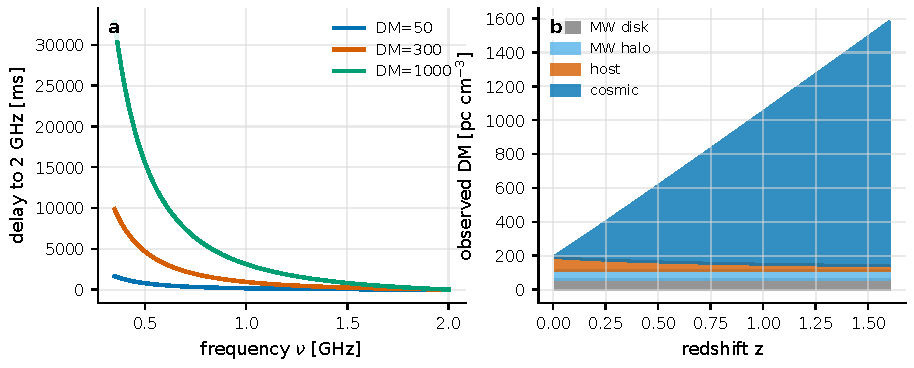
\includegraphics[width=0.94\linewidth]{figures/generated/chapter_14/ch14_dispersion_delay.pdf}
\caption{冷等离子体色散和 FRB 的 DM 预算。左图把到达时间延迟画成频率函数，参考频率为 \(2\,{\rm GHz}\)；低频端的 \(\nu^{-2}\) 斜率使 DM 很容易从宽带动态谱中估计。右图把一个局域 FRB 的观测 DM 拆成银河系盘、银晕、宿主星系和宇宙学等离子体贡献；宿主项因宇宙学时间膨胀按 \((1+z)^{-1}\) 进入观测值，宇宙学项在 \(z\lesssim1\) 近似随红移增长。}
\label{fig:ch14-dispersion}
\end{figure}

银河系电子密度远非一个常数。NE2001 把厚盘、薄盘、旋臂、局部空洞和团块组合起来，用脉冲星 DM、独立距离和散射数据约束参数；YMW16 更新了厚盘、薄盘、旋臂、银河中心和 Magellanic Clouds/IGM 处理，用来把脉冲星或 FRB 的银河系 DM 转换成距离或前景估计 \citep{2002astro.ph..7156C,2017ApJ...835...29Y}。高银纬视线的银河系盘 DM 常为 \(30-100\,{\rm pc\,cm^{-3}}\)，银晕贡献常取 \(50-100\,{\rm pc\,cm^{-3}}\) 的数量级；靠近银盘、HII 区或超新星遗迹时，局部结构会比平滑模型更重要。

宇宙学 FRB 常写成
\begin{equation}
  {\rm DM}_{\rm FRB}
  =
  {\rm DM}_{\rm MW,ISM}
  +{\rm DM}_{\rm MW,halo}
  +{\rm DM}_{\rm cosmic}(z)
  +\frac{{\rm DM}_{\rm host}}{{1+z}} .
  \label{eq:ch14-frb-dm-budget}
\end{equation}
\begin{formulaexplain}[公式 (14.7) 解读]
\({\rm DM}_{\rm FRB}\) 被拆成银河系盘、银晕、宇宙学等离子体和宿主星系四部分。这个预算式的意义是把一次 FRB 的总色散量变成沿途不同结构的电子柱密度账本。
\end{formulaexplain}
宿主星系项除以 \(1+z\)，因为观测到的频率和时间间隔已经被红移拉伸。均匀宇宙近似下
\begin{equation}
  {\rm DM}_{\rm cosmic}(z)
  =
  \frac{3cH_0\Omega_b f_{\rm IGM}}{8\pi Gm_p}
  \int_0^z
  \frac{f_e(z')(1+z')}{\sqrt{\Omega_m(1+z')^3+\Omega_\Lambda}}
  {\rm d}z' ,
  \label{eq:ch14-cosmic-dm}
\end{equation}
\begin{formulaexplain}[公式 (14.8) 解读]
\({\rm DM}_{\rm cosmic}\) 是宇宙学大尺度结构贡献，积分变量 \(z'\) 沿红移累加自由电子。前面的系数给出平均重子密度，积分核描述膨胀宇宙中电子数和路径长度如何随红移变化。
\end{formulaexplain}
\(\Omega_b\) 是重子密度参数，\(f_{\rm IGM}\) 是进入弥散 IGM 的重子比例，\(f_e\) 是每个重子的自由电子数。局域 FRB 样本给出的 \({\rm DM}_{\rm cosmic}\)-\(z\) 关系已经能测量宇宙重子含量；实际散布来自 cosmic web 的非均匀性，常用 \(\sigma_{\rm DM}\simeq F z^{-1/2}\) 的形式描述，\(F\sim0.1-0.4\) 对应不同 baryon feedback 和 halo gas 分布 \citep{2020Natur.581..391M,2014ApJ...790..101S}。

磁化等离子体使左右圆偏振的相速度不同，线偏振角随波长平方旋转：
\begin{equation}
  \psi(\lambda)=\psi_0+{\rm RM}\,\lambda^2 ,
  \label{eq:ch14-rm-angle}
\end{equation}
\begin{formulaexplain}[公式 (14.9) 解读]
\(\psi\) 是线偏振角，\(\psi_0\) 是本征偏振角，RM 是旋转量。偏振角对 \(\lambda^2\) 的斜率就是 RM，因此多频偏振观测能直接读出磁化等离子体的累积效应。
\end{formulaexplain}
\begin{equation}
  {\rm RM}
  =
  0.812
  \int
  \left(\frac{n_e}{{\rm cm^{-3}}}\right)
  \left(\frac{B_\parallel}{\mu{\rm G}}\right)
  \left(\frac{{\rm d}l}{\rm pc}\right)
  {\rm rad\,m^{-2}} .
  \label{eq:ch14-rm-definition}
\end{equation}
\begin{formulaexplain}[公式 (14.10) 解读]
RM 是 \(n_e\) 与视线磁场 \(B_\parallel\) 的路径积分。它不同于 DM：DM 只数电子，RM 还保留磁场方向信息，所以磁场反转会让 RM 互相抵消。
\end{formulaexplain}
\(B_\parallel\) 是指向观测者的磁场分量。若 DM 和 RM 主要来自同一区域，视线平均磁场可估为
\begin{equation}
  \langle B_\parallel\rangle
  \simeq
  1.232\,\mu{\rm G}\,
  \frac{{\rm RM}/{\rm rad\,m^{-2}}}{{\rm DM}/{\rm pc\,cm^{-3}}}.
  \label{eq:ch14-bfield-rm-dm}
\end{equation}
\begin{formulaexplain}[公式 (14.11) 解读]
\(\langle B_\parallel\rangle\) 是由 RM/DM 推出的电子加权平均磁场。这个估计只有在 RM 和 DM 来自同一段介质时才有直接物理含义。
\end{formulaexplain}
这不是一个普适磁场测量：若 RM 来自磁化宿主星系而 DM 大部分来自 IGM，式 \eqref{eq:ch14-bfield-rm-dm} 会低估局部磁场；若视线中有磁场反转，RM 会相互抵消而 DM 不会。星系团和星系际介质的 RM 研究常把这类退化与 X 射线气体密度、射电 halo 和背景源网格结合起来处理 \citep{2002ARA&A..40..319C}。

\begin{figure}[tbp]
\centering
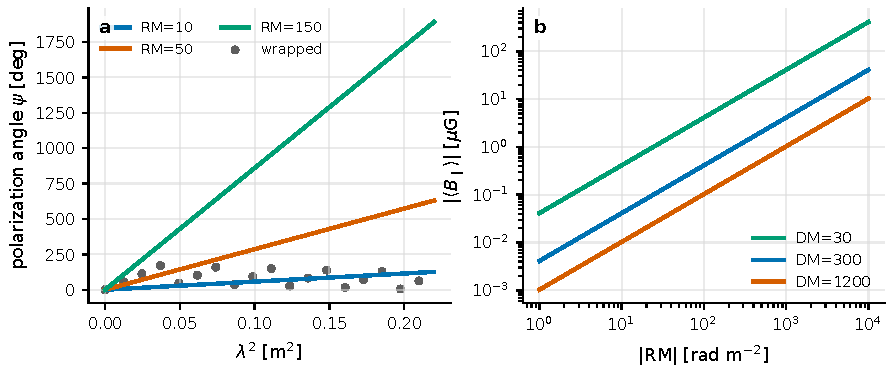
\includegraphics[width=0.94\linewidth]{figures/generated/chapter_14/ch14_faraday_rotation.pdf}
\caption{Faraday 旋转的两个读法。左图展示 \(\psi=\psi_0+{\rm RM}\lambda^2\) 的线性关系；黑点显示实际偏振角只在模 \(\pi\) 意义下测得，窄带数据容易出现缠绕歧义。右图把 \(\langle B_\parallel\rangle=1.232\,{\rm RM}/{\rm DM}\) 画成 RM 的函数；同一 RM 在低 DM 介质中代表更强的平均磁场。}
\label{fig:ch14-faraday}
\end{figure}

\section{散射、闪烁和尘埃怎样重排到达概率}

色散和 Faraday 旋转主要改变不同频率、不同偏振之间的相对相位或延迟；散射和尘埃更进一步，直接改变光子到达某个时间、方向、波长和偏振通道的概率。星际电子密度不是平滑函数。湍流中的小尺度起伏把波前打皱，结果是角展宽、脉冲展宽和强度闪烁。若源的本征强度是 \(I_{\rm src}(t)\)，单个薄屏近似常把观测脉冲写成卷积
\begin{equation}
  I_{\rm obs}(t)
  =
  \int I_{\rm src}(t')\,P(t-t')\,{\rm d}t',
  \qquad
  P(t)=\frac{1}{\tau_{\rm sc}}\exp\!\left(-\frac{t}{\tau_{\rm sc}}\right)H(t),
  \label{eq:ch14-scattering-convolution}
\end{equation}
\begin{formulaexplain}[公式 (14.12) 解读]
\(I_{\rm obs}\) 是观测强度，\(I_{\rm src}\) 是源端强度，\(P(t)\) 是散射到达时间核。单侧指数核表示光只能被延迟到达，不能提前到达，所以窄脉冲会变成长尾。
\end{formulaexplain}
\(P(t)\) 是一侧指数散射核，\(H(t)\) 是 Heaviside 函数。真实视线可有多个屏、各向异性散射和有限源尺寸，指数尾只是最常用的低阶模型。散射时间常写成
\begin{equation}
  \tau_{\rm sc}\propto \nu^{-\alpha},
  \label{eq:ch14-scattering-power}
\end{equation}
\begin{formulaexplain}[公式 (14.13) 解读]
\(\tau_{\rm sc}\) 是散射展宽时间，\(\alpha\) 是频率指数。指数越大，低频散射尾增长越快；这也是低频脉冲搜索容易丢失窄结构的原因。
\end{formulaexplain}
Kolmogorov 湍流薄屏给 \(\alpha\simeq4.4\)，多频脉冲星样本给出的经验平均更接近 \(\alpha=3.9\pm0.2\)，并且在固定 DM 下有超过一个数量级的散布 \citep{1977ARA&A..15..479R,1990ARA&A..28..561R,1995ApJ...443..209A,2004ApJ...605..759B}。常用经验式为
\begin{equation}
  \log_{10}\!\left(\frac{\tau_{\rm sc}}{{\rm ms}}\right)
  =
  -6.46
  +0.154\log_{10}{\rm DM}
  +1.07(\log_{10}{\rm DM})^2
  -3.86\log_{10}\!\left(\frac{\nu}{\rm GHz}\right),
  \label{eq:ch14-bhat-scattering}
\end{equation}
\begin{formulaexplain}[公式 (14.14) 解读]
这是一条经验散射关系，把 \(\tau_{\rm sc}\) 与 DM 和观测频率 \(\nu\) 联系起来。它适合做数量级预估，但真实视线的湍流结构会带来很大的散布。
\end{formulaexplain}
其中 DM 用 \({\rm pc\,cm^{-3}}\)。这条式子适合估计数量级，不适合替代每条视线的散射测量。对 \({\rm DM}=300\,{\rm pc\,cm^{-3}}\)，它给出 \(1.4\,{\rm GHz}\) 下约 ms 级的展宽；降到 \(600\,{\rm MHz}\) 时，展宽可增加到十几 ms 或更高。动态谱中的去相关带宽 \(\Delta\nu_d\) 与时间展宽近似满足
\begin{equation}
  \tau_{\rm sc}\simeq \frac{C_1}{2\pi\Delta\nu_d},
  \label{eq:ch14-decorrelation-bandwidth}
\end{equation}
\begin{formulaexplain}[公式 (14.15) 解读]
\(\Delta\nu_d\) 是闪烁去相关带宽，\(C_1\) 是几何相关的常数。时间展宽越长，频域中的相关带宽越窄；时间和频率是同一个多路径延迟分布的两种投影。
\end{formulaexplain}
\(C_1\) 是与几何和散射谱有关的常数，通常为 1 附近。强散射时，\(\Delta\nu_d\) 很窄，宽带平均会抹平闪烁；弱散射时，闪烁图样随时间和频率漂移，反而能测量屏速度、屏距离和源角尺寸。

\begin{figure}[tbp]
\centering
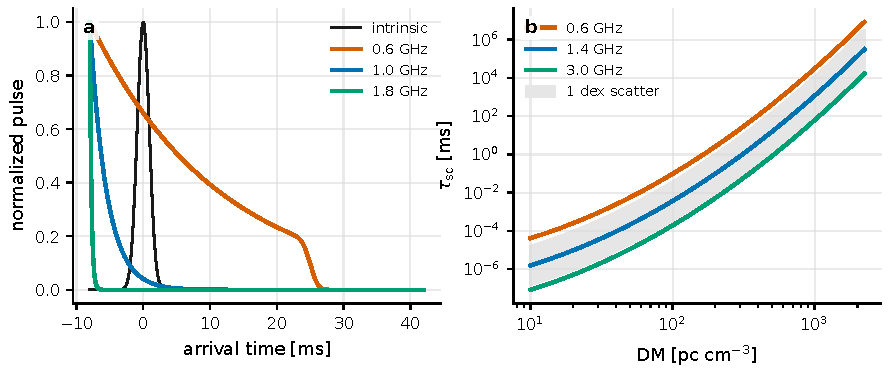
\includegraphics[width=0.94\linewidth]{figures/generated/chapter_14/ch14_scattering_broadening.pdf}
\caption{星际散射把短脉冲变成带长尾的到达时间分布。左图把一个窄高斯脉冲与一侧指数核卷积；频率越低，\(\tau_{\rm sc}\propto\nu^{-4}\) 使尾部越长。右图使用经验关系画出 \(\tau_{\rm sc}\) 随 DM 和频率的变化；灰色带表示固定 DM 下常见的数量级散布。}
\label{fig:ch14-scattering}
\end{figure}

等离子体还可以像透镜一样折射。横向电子柱密度梯度给出频率依赖的相位屏，低频光线偏折更强，强度可出现 caustic、multiple imaging 和 narrow-band 放大。高斯 plasma lens、FRB 宿主星系 plasma structures，以及非均匀等离子体中的引力透镜修正都表明，去掉 \(\nu^{-2}\) 色散以后，剩余结构仍可能来自传播过程 \citep{1998ApJ...496..253C,2010MNRAS.404.1790B,2014MNRAS.437.2180E,2017ApJ...842...35C}。在银河中心方向，毫米 VLBI 也要面对强散射屏；Sgr A* 的事件视界尺度成像需要同时处理本征结构、散射模糊和时间变化 \citep{2008Natur.455...78D,2022ApJ...930L..14E,2022ApJ...930L..15E}。

尘埃对光学和红外光子的影响更像一个带波长和偏振选择的损耗通道。通量关系为
\begin{equation}
  F_{\lambda,{\rm obs}}
  =
  F_{\lambda,{\rm int}}\,10^{-0.4A_\lambda},
  \label{eq:ch14-extinction-flux}
\end{equation}
\begin{formulaexplain}[公式 (14.16) 解读]
\(F_{\lambda,{\rm int}}\) 是本征通量，\(F_{\lambda,{\rm obs}}\) 是消光后的通量，\(A_\lambda\) 是波长相关消光。星等中的 \(0.4A_\lambda\) 转成指数衰减，表示尘埃按波长选择性吸收和散射光子。
\end{formulaexplain}
\(A_\lambda\) 的单位是 mag。选择性消光写成
\begin{equation}
  E(B-V)=A_B-A_V,
  \qquad
  R_V=\frac{A_V}{E(B-V)}.
  \label{eq:ch14-rv-definition}
\end{equation}
\begin{formulaexplain}[公式 (14.17) 解读]
\(E(B-V)\) 是蓝光和可见光消光差，\(R_V\) 把总消光与选择性红化相连。\(R_V\) 越大，消光曲线通常越灰，说明较大尘埃颗粒贡献更重要。
\end{formulaexplain}
银河系平均 \(R_V\simeq3.1\)，弥散 ISM 常在 \(2.5-3.5\) 附近，致密云中可到 \(5\) 以上，表示大颗粒使消光更灰。Cardelli-Clayton-Mathis 消光律把红外、光学和紫外平均曲线写成一个 \(R_V\) 参数族；Fitzpatrick 给出了实际视线中仍然存在的明显散布，尤其是 \(2175\,\text{\AA}\) bump 和 far-UV rise 的强弱 \citep{1989ApJ...345..245C,1999PASP..111...63F,2003ARA&A..41..241D}。若用平均消光律修正一个 \(E(B-V)=0.2\) mag 的蓝色源，紫外误差达到 \(0.1\) mag 并不奇怪；对偏振角、颜色温度和瞬变源早期谱能量分布，这已经是主要系统误差。

非球形尘埃颗粒在磁场中部分取向，会让通过的星光线偏振。常用 Serkowski 关系为
\begin{equation}
  \frac{P(\lambda)}{P_{\max}}
  =
  \exp\!\left[-K\ln^2\!\left(\frac{\lambda_{\max}}{\lambda}\right)\right],
  \label{eq:ch14-serkowski}
\end{equation}
\begin{formulaexplain}[公式 (14.18) 解读]
\(P(\lambda)\) 是尘埃造成的线偏振度，\(P_{\max}\) 是峰值，\(\lambda_{\max}\) 是峰值波长，\(K\) 控制曲线宽度。它把偏振随波长的形状和尘埃颗粒尺寸、取向环境联系起来。
\end{formulaexplain}
\(\lambda_{\max}\) 通常接近 \(0.55\,\mu{\rm m}\)，\(P_{\max}\) 的经验上限约为 \(9E(B-V)\%\)。这个上限不是每条视线都会达到；它受颗粒形状、取向效率、磁场方向变化和多云层叠加影响 \citep{1975ApJ...196..261S,2015ARA&A..53..501A}。尘埃散射还会把短暂爆发变成光回声或 X 射线 halo。若尘埃屏位于源到观测者距离的分数 \(x\)，散射角为 \(\theta\)，几何延迟近似
\begin{equation}
  \Delta t_{\rm dust}
  \simeq
  \frac{D_s}{2c}\frac{x}{1-x}\theta^2 ,
  \label{eq:ch14-dust-delay}
\end{equation}
\begin{formulaexplain}[公式 (14.19) 解读]
\(\Delta t_{\rm dust}\) 是尘埃散射造成的几何延迟，\(D_s\) 是源距离，\(x\) 是尘埃屏的相对位置，\(\theta\) 是散射角。延迟随 \(\theta^2\) 增长，因此角分辨光回声能反推出尘埃几何。
\end{formulaexplain}
\(D_s\) 是源距离。对银河系源，角秒级散射可给出小时到天的延迟；对银河系外源，尘埃几何和角分辨率要一起进入模型。

\begin{figure}[tbp]
\centering
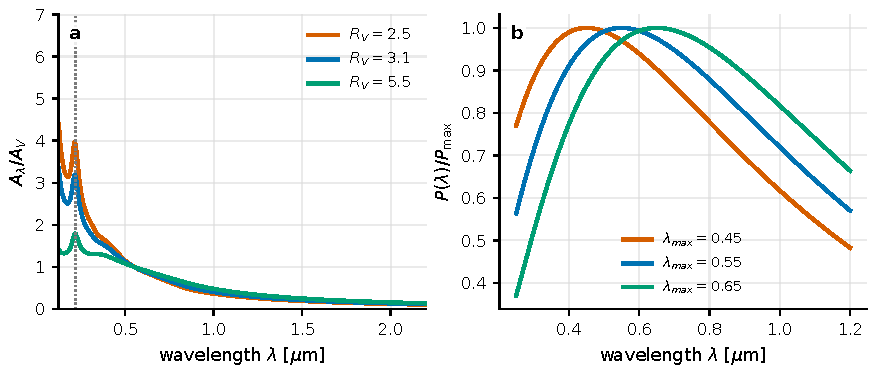
\includegraphics[width=0.94\linewidth]{figures/generated/chapter_14/ch14_dust_extinction_polarization.pdf}
\caption{尘埃改变光子的颜色、通量和偏振。左图是 CCM 平均消光曲线，\(R_V\) 越大，光学到近红外消光越灰；\(0.2175\,\mu{\rm m}\) 附近的紫外 bump 是小颗粒和碳质材料的重要诊断。右图是 Serkowski 偏振曲线，\(\lambda_{\max}\) 的移动反映颗粒尺寸和取向环境变化。}
\label{fig:ch14-dust}
\end{figure}

\section{引力透镜怎样把一条路径变成多条路径}

等离子体和尘埃来自真实介质；引力透镜来自弯曲时空。它不改变光子的频率色散关系，但改变路径、方向和到达时间。对事件表来说，透镜的核心动作很简单：一个源事件可以变成多个像、多个到达时刻和多个放大权重。薄透镜近似下
\begin{equation}
  {\boldsymbol\beta}
  =
  {\boldsymbol\theta}
  -
  {\boldsymbol\alpha}({\boldsymbol\theta}),
  \label{eq:ch14-lens-equation}
\end{equation}
\begin{formulaexplain}[公式 (14.20) 解读]
\({\boldsymbol\beta}\) 是源的真实角位置，\({\boldsymbol\theta}\) 是像位置，\({\boldsymbol\alpha}\) 是约化偏折角。透镜方程说明观测到的像不是源的直接方向，而是被质量分布偏折后的解。
\end{formulaexplain}
\({\boldsymbol\beta}\) 是真实源位置，\({\boldsymbol\theta}\) 是像位置，\({\boldsymbol\alpha}\) 是约化偏折角，三者常用角单位 rad 或 arcsec。点质量透镜的 Einstein 角为
\begin{equation}
  \theta_E
  =
  \left(
  \frac{4GM}{c^2}
  \frac{D_{ls}}{D_lD_s}
  \right)^{1/2}.
  \label{eq:ch14-einstein-angle}
\end{equation}
\begin{formulaexplain}[公式 (14.21) 解读]
\(\theta_E\) 是 Einstein 角，\(M\) 是透镜质量，\(D_l,D_s,D_{ls}\) 是角直径距离组合。它给出强透镜和微透镜的自然角尺度，也决定多像分离的量级。
\end{formulaexplain}
\(D_l\)、\(D_s\)、\(D_{ls}\) 是角直径距离。\(M=1\,M_\odot\)、银河系尺度几何给出 mas 量级的 \(\theta_E\)；星系质量透镜给出 arcsec 量级的多像分离。放大率为
\begin{equation}
  \mu
  =
  \frac{1}{\det(\partial{\boldsymbol\beta}/\partial{\boldsymbol\theta})},
  \label{eq:ch14-magnification}
\end{equation}
\begin{formulaexplain}[公式 (14.22) 解读]
\(\mu\) 是放大率，分母是从像平面到源平面的 Jacobian 行列式。行列式趋近零时，像面积被强烈拉伸，caustic 附近就会出现高放大。
\end{formulaexplain}
caustic 附近 \(|\mu|\) 可很大，但有限源尺寸、微透镜、尘埃和时间采样会限制实际可观测峰值。

到达时间由 Fermat 势控制：
\begin{equation}
  t({\boldsymbol\theta},{\boldsymbol\beta})
  =
  \frac{D_{\Delta t}}{c}
  \left[
  \frac{1}{2}|{\boldsymbol\theta}-{\boldsymbol\beta}|^2
  -
  \psi({\boldsymbol\theta})
  \right],
  \qquad
  D_{\Delta t}
  =
  (1+z_l)\frac{D_lD_s}{D_{ls}} .
  \label{eq:ch14-fermat-delay}
\end{equation}
\begin{formulaexplain}[公式 (14.23) 解读]
\(t({\boldsymbol\theta},{\boldsymbol\beta})\) 是相对到达时间，括号内第一项是几何路径差，\(\psi\) 是引力势延迟，\(D_{\Delta t}\) 是时间延迟距离。像的位置对应 Fermat 势的驻点。
\end{formulaexplain}
\(\psi\) 是二维透镜势，\(D_{\Delta t}\) 是时间延迟距离。两幅像之间的观测延迟为
\begin{equation}
  \Delta t_{AB}
  =
  \frac{D_{\Delta t}}{c}\,
  \Delta\phi_{AB}.
  \label{eq:ch14-time-delay-distance}
\end{equation}
\begin{formulaexplain}[公式 (14.24) 解读]
\(\Delta t_{AB}\) 是两幅像的到达时间差，\(\Delta\phi_{AB}\) 是 Fermat 势差。观测延迟乘上透镜模型后给出 \(D_{\Delta t}\)，因此可以约束 \(H_0\)。
\end{formulaexplain}
星系强透镜的 \(\Delta t_{AB}\) 常为天到月，少数系统可到年；它只占 \(D_{\Delta t}/c\) 的 \(10^{-11}\) 左右，因此透镜势、外部收敛、质量片退化和光变曲线采样都会直接进入 \(H_0\) 误差预算。Refsdal 首先指出多像时间延迟可测 \(H_0\)；现代 time-delay cosmography 依赖多年监测、高分辨成像、透镜星系速度弥散和环境建模 \citep{1964MNRAS.128..295R,1964MNRAS.128..307R,1986ApJ...310..568B,2016A&ARv..24...11T}。

\begin{figure}[tbp]
\centering
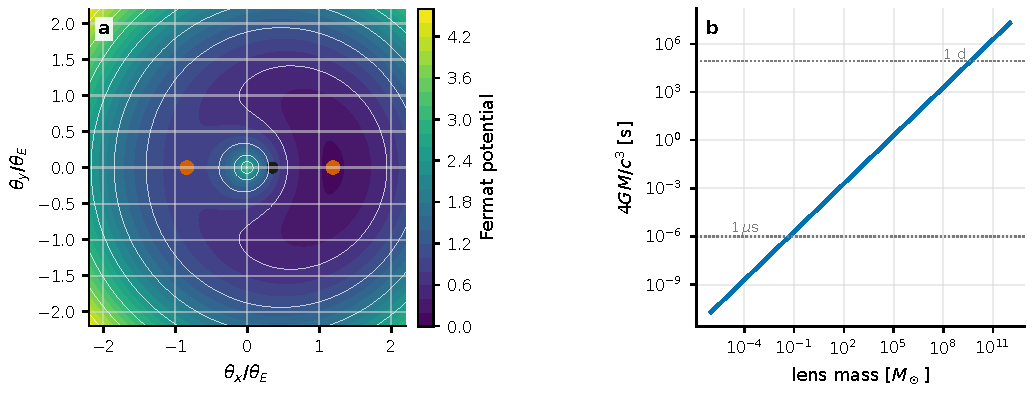
\includegraphics[width=0.94\linewidth]{figures/generated/chapter_14/ch14_lensing_time_delay.pdf}
\caption{强透镜的两个尺度。左图是点质量透镜的 Fermat 到达时间面，黑点是源位置，两个橙点是像位置；像出现在到达时间面的驻点。右图给出 \(4GM/c^3\) 的基本延迟尺度：恒星质量透镜对应微秒到毫秒，星系和星系团透镜自然进入天到年的时间域。}
\label{fig:ch14-lensing}
\end{figure}

当波长不能忽略时，几何光学的“多条光线”要改成波的衍射积分。对引力波透镜常用无量纲频率
\begin{equation}
  w
  =
  \frac{8\pi GM(1+z_l)f}{c^3}.
  \label{eq:ch14-wave-lensing-w}
\end{equation}
\begin{formulaexplain}[公式 (14.25) 解读]
\(w\) 是波动光学透镜的无量纲频率，\(M\) 是透镜质量，\(f\) 是波频率。\(w\) 比较的是波的周期和透镜引起的时间尺度：大 \(w\) 近似几何光学，小 \(w\) 必须考虑衍射。
\end{formulaexplain}
\(w\gg1\) 时回到几何光学，多像可分开并产生相干干涉条纹；\(w\lesssim1\) 时衍射抹平 caustic，放大率不再能用几何像简单相加。频域波形写为
\begin{equation}
  \tilde h_L(f)=F(f)\,\tilde h(f),
  \label{eq:ch14-wave-amplification}
\end{equation}
\begin{formulaexplain}[公式 (14.26) 解读]
\(\tilde h(f)\) 是未透镜波形，\(\tilde h_L(f)\) 是透镜后的频域波形，\(F(f)\) 是复放大因子。它同时包含振幅放大和相位延迟，所以可以产生频率依赖的干涉结构。
\end{formulaexplain}
\(F(f)\) 是复放大因子。若两条路径延迟为 \(\Delta t\)，干涉条纹的频率间隔约为
\begin{equation}
  \Delta f \simeq \frac{1}{\Delta t}.
  \label{eq:ch14-lensing-fringe-spacing}
\end{equation}
\begin{formulaexplain}[公式 (14.27) 解读]
\(\Delta f\) 是频域条纹间距，\(\Delta t\) 是两条路径的时间延迟。路径延迟越长，频域振荡越密；这把时间结构转写成谱中的干涉条纹。
\end{formulaexplain}
例如 \(\Delta t=2\,{\rm ms}\) 时，条纹间隔约 \(500\,{\rm Hz}\)。对电磁光学频率，普通恒星或星系质量透镜通常 \(w\) 极大，几何光学非常好；对 LISA 频段引力波和 \(10^6-10^9M_\odot\) 透镜，波动光学效应可以进入观测带 \citep{2003ApJ...595.1039T}。

\begin{figure}[tbp]
\centering
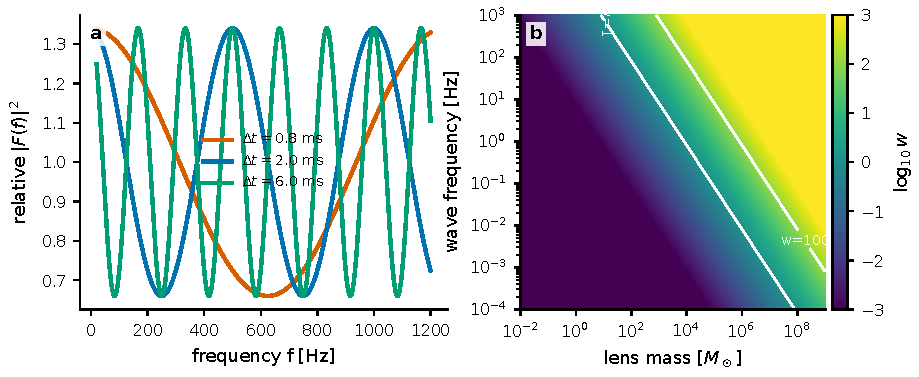
\includegraphics[width=0.94\linewidth]{figures/generated/chapter_14/ch14_wave_lensing_interference.pdf}
\caption{波动光学透镜把时间延迟变成频域条纹。左图画出不同路径延迟下的相对放大因子振荡，\(\Delta f\simeq1/\Delta t\)。右图给出 \(w=8\pi GMf/c^3\) 的量级；白线 \(w=1\) 附近是衍射与几何光学的过渡，\(w=100\) 以上通常可把像当成独立路径处理。}
\label{fig:ch14-wave-lensing}
\end{figure}

\section{相关函数和 cosmic Bell 的边界在哪里}

前面几节把传播写成对单个事件标签的改写。最后要回到本书主线：相关函数。多路径传播会重排强度相关，因为观测到的涨落不一定来自源端同一时刻；它可能是同一个源端结构沿不同路径晚到、早到或被放大后的叠加。若透镜或散射在观测带内可近似为若干离散路径，
\begin{equation}
  h(t)=\sum_i \sqrt{\mu_i}\,e^{i\varphi_i}\delta(t-t_i),
  \label{eq:ch14-multipath-impulse}
\end{equation}
\begin{formulaexplain}[公式 (14.28) 解读]
\(h(t)\) 是多路径脉冲响应，\(\mu_i\) 是第 \(i\) 条路径放大率，\(\varphi_i\) 是相位，\(t_i\) 是到达延迟。每个 delta 函数代表一条可分辨路径。
\end{formulaexplain}
\(\mu_i\) 是第 \(i\) 条路径的放大率，\(\varphi_i\) 是相位，\(t_i\) 是到达时间。若相位在带宽或源尺寸上被平均掉，观测强度近似
\begin{equation}
  I_{\rm obs}(t)
  =
  \sum_i \mu_i I_{\rm src}(t-t_i).
  \label{eq:ch14-multipath-intensity}
\end{equation}
\begin{formulaexplain}[公式 (14.29) 解读]
\(I_{\rm obs}\) 是观测强度，\(I_{\rm src}\) 是源端强度。相位平均后，不同路径的强度按放大率加权相加，因此一个源端变化会在多个延迟处重复出现。
\end{formulaexplain}
对强度涨落 \(\delta I=I-\langle I\rangle\)，自相关函数
\begin{equation}
  C_{\rm obs}(\tau)
  =
  \left\langle
  \delta I_{\rm obs}(t)\,
  \delta I_{\rm obs}(t+\tau)
  \right\rangle
  =
  \sum_{ij}\mu_i\mu_j
  C_{\rm src}\!\left(\tau+t_i-t_j\right)
  \label{eq:ch14-correlation-echo}
\end{equation}
\begin{formulaexplain}[公式 (14.30) 解读]
\(C_{\rm obs}\) 是观测强度自相关，\(C_{\rm src}\) 是源端自相关。双重求和表示每一对路径都会贡献一个相关回声，回声位置由两条路径的延迟差决定。
\end{formulaexplain}
会在 \(\tau=t_j-t_i\) 附近出现回声结构。这个关系只在源本身有可测快速结构、传播路径稳定、观测时间覆盖足够长、背景和选择函数已经建模时有用。热光的 \(g^{(2)}(0)\) 峰、脉冲星 giant pulse 的微结构、FRB 的窄带 scintillation 和透镜多像延迟都可落入这个框架，但它们的相干时间、带宽和统计分布不同；相关峰本身还不足以确定物理来源。

传播效应也定义了 cosmic Bell test 的适用边界。实验室 Bell 检验使用纠缠光子对，两个站点选择测量设置 \(a,a'\) 和 \(b,b'\)，CHSH 组合为
\begin{equation}
  S
  =
  E(a,b)+E(a,b')+E(a',b)-E(a',b'),
  \qquad
  |S|\le 2
  \label{eq:ch14-chsh}
\end{equation}
\begin{formulaexplain}[公式 (14.31) 解读]
\(S\) 是 CHSH 组合，\(E(a,b)\) 是给定测量设置下的相关期望值。局域隐变量模型要求 \(|S|\le2\)；cosmic Bell 实验用天文光子选择设置，是为了把可能共同原因推到更早的宇宙时刻。
\end{formulaexplain}
是局域隐变量模型的上限。cosmic Bell 实验用银河系恒星或高红移类星体光子实时决定 \(a\) 和 \(b\)，目的是把可能共同原因推到更早的时空区域，而不是证明天体光子本身处在纠缠态。Milky Way stars 版本使用星光颜色产生设置并处理大气延迟、探测噪声和错误设置概率；quasar 版本进一步把自由选择漏洞的共同过去推到宇宙早期 \citep{2017PhRvL.118f0401H,2018PhRvL.121h0403R}。这类实验检验的是因果结构：天文光子可以参与量子基础实验的设置选择，但传播中的吸收、红化、色散和仪器延迟要逐项进入实验时序。

\begin{figure}[tbp]
\centering
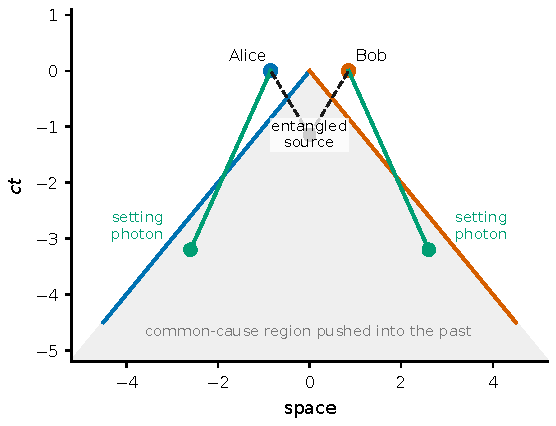
\includegraphics[width=0.72\linewidth]{figures/generated/chapter_14/ch14_cosmic_bell_lightcones.pdf}
\caption{Cosmic Bell 实验的光锥结构。纠缠源在本地实验中发出光子对，Alice 和 Bob 的测量设置由远处恒星或类星体光子决定；这些设置光子的发射事件越早、方向分离越大，可能共同原因被排除的时空区域越大。图中灰区表示被推向过去的共同原因区域，实际实验还要加入大气传播、探测器响应和电子延迟。}
\label{fig:ch14-cosmic-bell}
\end{figure}

普通传播效应给出了新物理搜索的误差地板。轴子样粒子可让光子在磁场中转化，宇宙双折射会旋转偏振，暗物质小结构可改写透镜放大率和时间延迟；这些解释需要先和等离子体、尘埃、透镜和仪器项放在同一个模型中比较。若剩余信号同时经得起时间、频率、偏振和角位置检验，才有资格作为新物理候选。


\chapter{暗物质、轴子和偏振量子通道}
\label{chap:15}

\begin{chapteropening}
暗物质和轻场新物理很少直接给出一张“新粒子图像”。它们更常出现在偏振角、到达时间、相关函数、透镜放大率和像位置的微小偏离里。轴子和轴子样粒子通过 \(aF\tilde F\) 耦合旋转线偏振或在外磁场中与光子转换；超轻暗物质可让这种旋转随时间振荡；黑洞超辐射可在 Kerr 黑洞附近堆积轻玻色云；冷暗物质小晕则通过透镜扰动改变多像系统。QCD axion 的基础、现代 axion cosmology、CAST helioscope、CMB cosmic birefringence、EHT 轴子云搜索和强透镜子结构测量给出了这些信号的主要观测入口 \citep{1977PhRvL..38.1440P,1978PhRvL..40..223W,1978PhRvL..40..279W,1983PhRvL..51.1415S,2016PhR...643....1M,2017NatPh..13..584C,1990PhRvD..41.1231C,1999PhRvL..83.1506L,2020PhRvL.125v1301M,2022NatRP...4..452K,2020PhRvL.124f1102C,2022NatAs...6..592C,1998MNRAS.295..587M,2002ApJ...572...25D}。
\end{chapteropening}

\section{轴子场怎样进入光子的偏振和强度}

这一章的基本态度是先把“新物理”翻译成观测量，再问普通天体物理和仪器能不能模仿它。对轴子和轴子样粒子来说，最常见的两个入口很直接：一个是偏振角被旋转，另一个是外磁场中轴子和光子相互转换，改变某个偏振态或能段的强度。二者都来自同一个相互作用项。

低能有效理论中，轴子样场 \(a\) 与电磁场的相互作用写成
\begin{equation}
  \mathcal L_{a\gamma}
  =
  -\frac{1}{4}g_{a\gamma}aF_{\mu\nu}\tilde F^{\mu\nu}
  =
  g_{a\gamma}a\,{\bf E}\cdot{\bf B}.
  \label{eq:ch15-axion-lagrangian}
\end{equation}
\begin{formulaexplain}[公式 (15.1) 解读]
\(\mathcal L_{a\gamma}\) 是轴子-光子耦合项，\(g_{a\gamma}\) 是耦合强度，\(a\) 是轴子样场，\(F_{\mu\nu}\) 和 \(\tilde F^{\mu\nu}\) 是电磁张量及其对偶。写成 \({\bf E}\cdot{\bf B}\) 后可以看出：这个相互作用只在偏振和磁场方向相关时显现。
\end{formulaexplain}
\(g_{a\gamma}\) 的单位是 \({\rm energy}^{-1}\)，天体和实验文献常用 \({\rm GeV^{-1}}\)。\(F_{\mu\nu}\) 是电磁张量，\(\tilde F^{\mu\nu}\) 是对偶张量；第二个等号把耦合写成 \({\bf E}\cdot{\bf B}\)，只有电场和磁场的相对取向带有手征信息时才起作用。QCD axion 还满足近似质量-衰变常数关系
\begin{equation}
  m_a \simeq
  5.7\,\mu{\rm eV}
  \left(\frac{10^{12}\,{\rm GeV}}{f_a}\right),
  \label{eq:ch15-qcd-axion-mass}
\end{equation}
\begin{formulaexplain}[公式 (15.2) 解读]
\(m_a\) 是 QCD axion 质量，\(f_a\) 是 PQ 对称破缺尺度。尺度越高，轴子越轻；这条关系把 QCD axion 限制在参数图上的一条窄带附近。
\end{formulaexplain}
其中 \(f_a\) 是 PQ 对称破缺尺度。ALP 不必满足这条关系，\(m_a\) 和 \(g_{a\gamma}\) 可以近似独立，因此图上常把 QCD axion band 和更宽的 ALP 参数空间分开 \citep{2016PhR...643....1M,2014JHEP...06..037D}。

外磁场中，轴子和与 \(B_\perp\) 平行的光子偏振态混合。弱混合、均匀磁场、吸收可忽略时，
\begin{equation}
  P_{a\to\gamma}
  \simeq
  \left(\frac{g_{a\gamma}B_\perp L}{2}\right)^2
  \mathrm{sinc}^2\!\left(\frac{qL}{2}\right),
  \qquad
  q\simeq \frac{|m_a^2-m_\gamma^2|}{2E}.
  \label{eq:ch15-axion-conversion}
\end{equation}
\begin{formulaexplain}[公式 (15.3) 解读]
\(P_{a\to\gamma}\) 是轴子转成光子的概率，\(B_\perp\) 是横向磁场，\(L\) 是相干长度，\(q\) 是轴子和光子动量失配。前面的平方项给强度，\(\mathrm{sinc}^2\) 项说明相位失配会破坏相干累积。
\end{formulaexplain}
\(B_\perp\) 是垂直于传播方向的磁场，\(L\) 是相干路径长度，\(E\) 是粒子能量，\(m_\gamma\) 是等离子体中光子的有效质量。\(qL\ll1\) 时振幅沿路径相干相加，概率按 \(L^2\) 增长；\(qL\gtrsim\pi\) 后，相位失配让不同路径段相互抵消。CAST 使用 \(9\,{\rm T}\)、\(9.26\,{\rm m}\) 的 LHC 退役偶极磁体寻找太阳 axion 转换成 X 射线；2013-2015 真空管数据给出 \(g_{a\gamma}<0.66\times10^{-10}\,{\rm GeV^{-1}}\) 的 95\% C.L. 限制，适用于 \(m_a\lesssim0.02\,{\rm eV}\) 的相干低质量区 \citep{2017NatPh..13..584C}。

\begin{figure}[tbp]
\centering
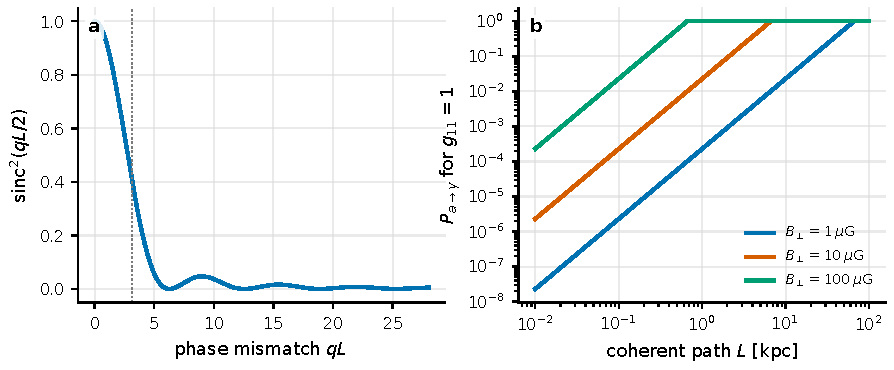
\includegraphics[width=0.94\linewidth]{figures/generated/chapter_15/ch15_axion_conversion.pdf}
\caption{轴子-光子转换由强度和相位共同控制。左图显示 \(\mathrm{sinc}^2(qL/2)\) 的相干因子；当 \(qL\) 接近 \(\pi\) 后，路径不同部分的转换振幅开始抵消。右图给出星际尺度的相干极限数量级，采用 \(g_{11}=g_{a\gamma}/10^{-11}{\rm GeV^{-1}}=1\)；在 \(\mu{\rm G}\) 磁场和 kpc 路径中，单段转换概率通常远小于 1。}
\label{fig:ch15-axion-conversion}
\end{figure}

同一个耦合也会让线偏振角旋转。若光子从发射点 \(e\) 到观测者 \(o\) 穿过缓慢变化的轴子背景，几何光学近似给出
\begin{equation}
  \Delta\psi
  =
  \frac{1}{2}g_{a\gamma}\,[a(t_o,{\bf x}_o)-a(t_e,{\bf x}_e)] .
  \label{eq:ch15-axion-rotation}
\end{equation}
\begin{formulaexplain}[公式 (15.4) 解读]
\(\Delta\psi\) 是线偏振角旋转，括号内是观测端和发射端轴子场的差。它不含 \(\lambda^2\)，因此和 Faraday 旋转最重要的区别是近似无波长依赖。
\end{formulaexplain}
这条旋转与波长无关，和第 \ref{chap:14} 章的 Faraday 旋转 \(\psi=\psi_0+{\rm RM}\lambda^2\) 不同。若轴子构成本地超轻暗物质，
\begin{equation}
  a(t,{\bf x})
  \simeq
  a_0\cos(m_at+\varphi),
  \qquad
  a_0=\frac{\sqrt{2\rho_a}}{m_a}.
  \label{eq:ch15-axion-dm-field}
\end{equation}
\begin{formulaexplain}[公式 (15.5) 解读]
\(a(t,{\bf x})\) 是经典振荡轴子场，\(a_0\) 是振幅，\(\rho_a\) 是轴子暗物质能量密度。质量越小，在同样能量密度下场振幅越大，偏振旋转的时间变化也越慢。
\end{formulaexplain}
\(\rho_a\) 是局部暗物质能量密度，银河系常用 \(0.3\,{\rm GeV\,cm^{-3}}\) 作数量级。振荡周期和相干时间为
\begin{equation}
  T_a
  =
  \frac{2\pi\hbar}{m_ac^2}
  \simeq
  47.9\,{\rm d}
  \left(\frac{10^{-21}\,{\rm eV}}{m_a}\right),
  \qquad
  t_{\rm coh}\sim \frac{T_a}{v^2},
  \label{eq:ch15-axion-timescales}
\end{equation}
\begin{formulaexplain}[公式 (15.6) 解读]
\(T_a\) 是轴子场振荡周期，\(t_{\rm coh}\) 是相干时间，\(v\) 是暗物质速度弥散。超轻质量对应长周期；速度弥散很小，所以同一频率相位可保持许多周期。
\end{formulaexplain}
其中 \(v\sim10^{-3}c\) 是银河系 halo 速度弥散。\(m_a=10^{-21}\,{\rm eV}\) 时，偏振角可在几十天周期上振荡，而相干时间可到 \(10^5\) 年量级。CMB axion dark matter 搜索利用今天本地场的共同振荡和最后散射面处的 washout 效应；Fedderke、Graham 和 Rajendran 指出，普通静态 cosmic birefringence 搜索并不等价于这种快速振荡信号 \citep{2019PhRvD.100a5040F,2021ARA&A..59..247H}。

\begin{figure}[tbp]
\centering
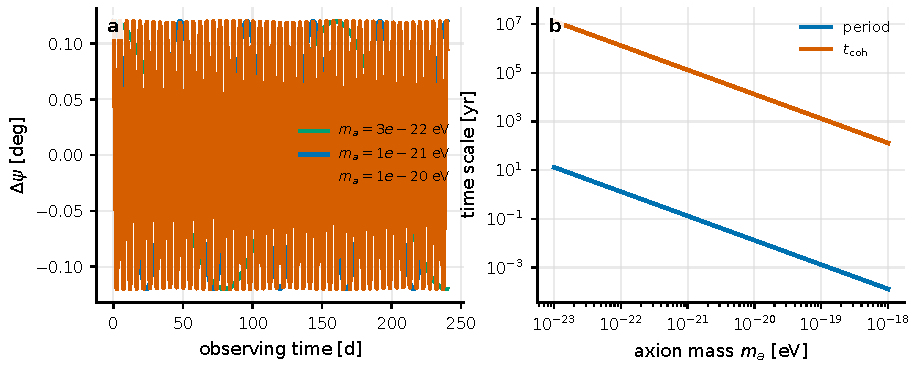
\includegraphics[width=0.94\linewidth]{figures/generated/chapter_15/ch15_axion_polarization_oscillation.pdf}
\caption{超轻暗物质把偏振旋转变成时间序列。左图画出三个轴子质量对应的 \(\Delta\psi(t)\)；质量越大，振荡越快。右图把 \(m_a\) 转换成周期 \(T_a\) 和相干时间 \(t_{\rm coh}\sim T_a/v^2\)，其中 \(v=10^{-3}c\)。}
\label{fig:ch15-axion-oscillation}
\end{figure}

\section{CMB 双折射为什么首先是角标定问题}

CMB 是寻找全局偏振旋转的诱人对象：最后散射面很远，天空覆盖大，统计量可以压到很小。但它也把一个简单问题变成最尖锐的系统误差问题。宇宙本身把偏振转过 \(\beta\)，和探测器偏振角整体错标 \(\alpha\)，在 CMB 谱里几乎长得一样。因而这一节的核心不是先宣布一个非零 \(\beta\)，而是看它怎样与角标定、银河尘埃和偏振泄漏分开。

线偏振 Stokes 参数 \(Q\) 和 \(U\) 旋转角 \(\beta\) 后，
\begin{equation}
  Q\pm iU \rightarrow e^{\pm2i\beta}(Q\pm iU).
  \label{eq:ch15-qu-rotation}
\end{equation}
\begin{formulaexplain}[公式 (15.7) 解读]
\(Q\) 和 \(U\) 是线偏振 Stokes 参数，\(\beta\) 是整体偏振旋转角。指数里的 \(2\beta\) 来自线偏振的自旋 2 性质，因此小角度误差会把 \(E\) 模和 \(B\) 模互相泄漏。
\end{formulaexplain}
在球谐空间中，这会把 \(E\) 模和 \(B\) 模混合。若最后散射面本征 \(EB\) 很小，观测到的 parity-odd 谱近似为
\begin{equation}
  C_\ell^{EB,{\rm obs}}
  =
  \frac{1}{2}\sin(4\beta)
  \left(C_\ell^{EE}-C_\ell^{BB}\right),
  \qquad
  C_\ell^{TB,{\rm obs}}
  =
  \sin(2\beta)C_\ell^{TE}.
  \label{eq:ch15-cmb-eb-tb}
\end{equation}
\begin{formulaexplain}[公式 (15.8) 解读]
\(C_\ell^{EB,{\rm obs}}\) 和 \(C_\ell^{TB,{\rm obs}}\) 是旋转后出现的奇宇称谱。若本征 \(EB/TB\) 很小，非零信号可由 \(\beta\) 产生，但探测器角标定误差也会产生几乎同样的形式。
\end{formulaexplain}
\(\beta=0.35^\circ\) 时，\(\sin(4\beta)/2\simeq0.012\)，所以 EB 泄漏是 EE-BB 差值的百分之一量级。Planck 2018 的重新分析通过 CMB 与银河前景偏振的不同频率和多极矩依赖，同时拟合 cosmic birefringence angle \(\beta\) 与 detector angle miscalibration \(\alpha\)，得到 \(\beta=0.35\pm0.14^\circ\) 的 68\% C.L. 结果；后续 WMAP+Planck 和 Planck PR4 分析指出，尘埃 EB、bandpass mismatch、\(I\to P\) leakage、cross-polarization response 和 mask 选择仍是主要系统误差 \citep{2020PhRvL.125v1301M,2022PhRvD.106f3503E,2022PhRvL.128i1302D,2022NatRP...4..452K}。

\begin{figure}[tbp]
\centering
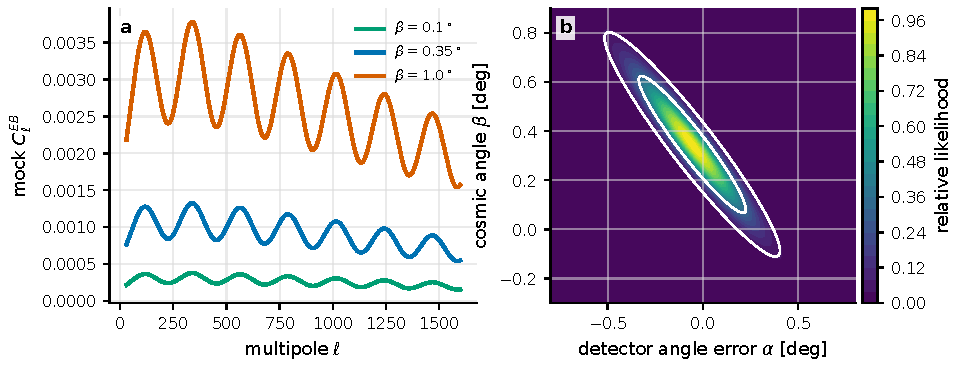
\includegraphics[width=0.94\linewidth]{figures/generated/chapter_15/ch15_cosmic_birefringence.pdf}
\caption{Cosmic birefringence 同时涉及 \(E/B\) 混合和仪器角标定。左图用 toy \(EE\) 与 \(BB\) 谱显示 \(\beta\) 如何产生 \(EB\)。右图显示 \(\alpha\) 与 \(\beta\) 的退化：若只看 CMB，探测器角误差和宇宙旋转几乎等价；利用前景频率依赖可以部分打破退化。}
\label{fig:ch15-cmb-birefringence}
\end{figure}

\Needspace{12\baselineskip}
单光子偏振事件表把这个问题从平均 map 推向时间域。一个偏振事件可写作
\begin{equation}
  e_q=(t_q,\nu_q,\hat{\bf n}_q,p_q,w_q),
  \label{eq:ch15-polarization-event}
\end{equation}
\begin{formulaexplain}[公式 (15.9) 解读]
\(e_q\) 是第 \(q\) 个偏振事件，包含时间、频率、方向、偏振通道和权重。把数据保留为事件表，可以在时间和频率维度上寻找共同旋转，而不必先平均成一张固定角度图。
\end{formulaexplain}
\(p_q\) 是偏振通道，\(w_q\) 是质量权重。若偏振角存在小的公共振荡，事件概率可以写成
\begin{equation}
  P(p_q|t_q,\nu_q,\hat{\bf n}_q)
  =
  P_0\!\left[p_q\,\middle|\,\psi_{\rm src}+\psi_{\rm prop}(\nu_q,\hat{\bf n}_q)+\delta\psi(t_q,\hat{\bf n}_q)\right].
  \label{eq:ch15-event-likelihood}
\end{equation}
\begin{formulaexplain}[公式 (15.10) 解读]
\(P_0\) 是给定总偏振角后的偏振通道概率，\(\psi_{\rm src}\) 是源本征项，\(\psi_{\rm prop}\) 是传播和仪器项，\(\delta\psi\) 是待检验的新物理旋转。这条式子把异常角度拆成可互相反驳的几类来源。
\end{formulaexplain}
\(\psi_{\rm src}\) 是源本征偏振，\(\psi_{\rm prop}\) 包括 Faraday、尘埃和仪器 Mueller 矩阵，\(\delta\psi\) 是要检验的新物理项。事件表可以在不同时间、频率和偏振通道之间做同一个似然，避免过早把数据平均成一个固定偏振角。代价也很直接：如果 Mueller 矩阵非对角项只知道到 \(10^{-3}\)，而目标旋转是 \(10^{-3}\,{\rm rad}\)，系统误差已经和信号同量级。强场 QED 真空双折射候选、孤立中子星光学偏振和 magnetar X-ray 偏振都要求先建模源几何和传播效应，偏振异常才可能被解释为新物理 \citep{2017MNRAS.465..492M}。

\section{脉冲星、FRB 和黑洞怎样提供前景检验}

CMB 给出全天平均的角度检验；脉冲星、FRB 和黑洞附近偏振则把问题推向时间域和强场环境。它们的优点是信号可以随时间、频率或黑洞尺度有特定模板；缺点是本征源结构和传播前景都很强。真正有用的策略，是把“共同时间项”“\(\lambda^2\) 前景”“黑洞质量标度”这些可区分特征放在同一个似然里。

脉冲星适合做时间域阵列，因为它们有稳定相位和重复脉冲。超轻标量暗物质的引力势振荡可在 PTA 中产生窄带 timing residual。若势扰动写成 \(\Psi_c\cos(2m_at+\varphi)\)，一个简化残差可写作
\begin{equation}
  R_\alpha(t)
  \simeq
  \frac{\Psi_c}{2\pi f}
  \left[
  \sin(2\pi ft+\varphi_E)
  -
  \sin(2\pi f(t-D_\alpha/c)+\varphi_\alpha)
  \right],
  \label{eq:ch15-pta-residual}
\end{equation}
\begin{formulaexplain}[公式 (15.11) 解读]
\(R_\alpha(t)\) 是第 \(\alpha\) 颗脉冲星的计时残差，\(\Psi_c\) 是势振荡幅度，\(f\) 是窄带频率。第一项是共同 Earth term，第二项是每颗脉冲星自己的 pulsar term。
\end{formulaexplain}
\(\alpha\) 标记第 \(\alpha\) 颗脉冲星，\(D_\alpha\) 是距离，\(f\simeq m_a/\pi\) 是势振荡频率。\(m_a\sim10^{-23}\,{\rm eV}\) 对应 \(f\sim10^{-8}\,{\rm Hz}\)，正好落在 PTA 的 \(10^{-9}-10^{-7}\,{\rm Hz}\) 窗口。Porayko 和 Postnov 对 NANOGrav 旧数据的分析给出 \(\Psi_c<1.14\times10^{-15}\) 的 95\% C.L. 上限，对应 \(f=1.75\times10^{-8}\,{\rm Hz}\) 处 \(h_c<4\times10^{-15}\) 的数量级 \citep{2014PhRvD..90f2008P}。在窄带随机背景近似中，不同脉冲星之间的相关可近似为
\begin{equation}
  \zeta_{\alpha\beta}=\frac{1}{2}(1+\delta_{\alpha\beta}),
  \label{eq:ch15-pta-correlation}
\end{equation}
\begin{formulaexplain}[公式 (15.12) 解读]
\(\zeta_{\alpha\beta}\) 是两颗脉冲星残差的相关系数，\(\delta_{\alpha\beta}\) 是 Kronecker delta。这个标量暗物质模板几乎不依赖两颗脉冲星的夹角，因此不同于张量引力波背景的 Hellings-Downs 曲线。
\end{formulaexplain}
这和随机引力波背景的 Hellings-Downs 角相关不同。若未来做“脉冲星偏振阵列”，同样要把共同 Earth term、本征磁层偏振、星际 Faraday 旋转、profile mode changes 和接收机偏振泄漏分开。

\begin{figure}[tbp]
\centering
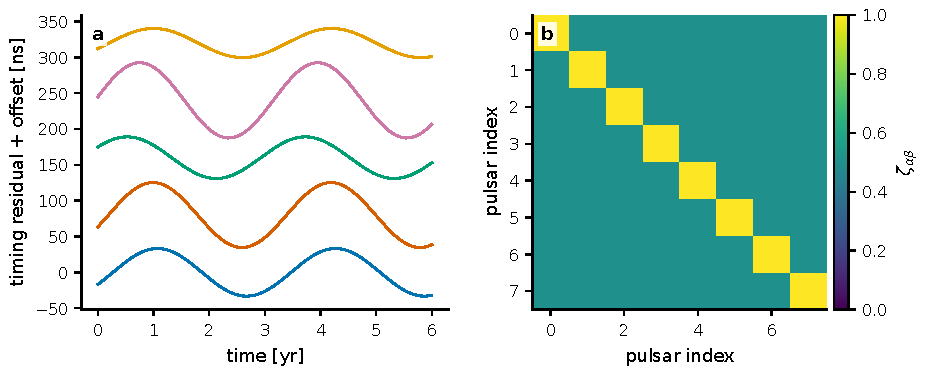
\includegraphics[width=0.94\linewidth]{figures/generated/chapter_15/ch15_pulsar_array_correlation.pdf}
\caption{脉冲星阵列里的共同窄带信号。左图是一个公共 Earth term 叠加每颗脉冲星自己的 pulsar term；曲线被人为错开以便观看。右图给出标量势振荡模型中的简化相关矩阵 \(\zeta_{\alpha\beta}=(1+\delta_{\alpha\beta})/2\)，它不同于随机张量引力波背景的角相关。}
\label{fig:ch15-pulsar-array}
\end{figure}

FRB 的偏振信息强，但传播前景也强。FRB 121102 在 \(z=0.193\) 的宿主星系中，4-8 GHz bursts 显示接近 \(100\%\) 线偏振，并有源框架 \({\rm RM}_{\rm src}=1.46\times10^5\) 和 \(1.33\times10^5\,{\rm rad\,m^{-2}}\) 的高而变化的 Faraday rotation measure；同一批 burst 还含有 \(\lesssim30\,\mu{\rm s}\) 的窄结构。若宿主贡献 \({\rm DM}_{\rm host}\sim70-270\,{\rm pc\,cm^{-3}}\)，对应的视线磁场下限为 mG 量级，远高于普通银河系 ISM 的 \(\sim5\,\mu{\rm G}\) \citep{2018Natur.553..182M}。这类源可作为极端磁化等离子体实验室；一个看似波长无关的偏振变化，仍要排除通道平均导致的 depolarization、RM 时间变化和 plasma lensing 选择效应。

\begin{figure}[tbp]
\centering
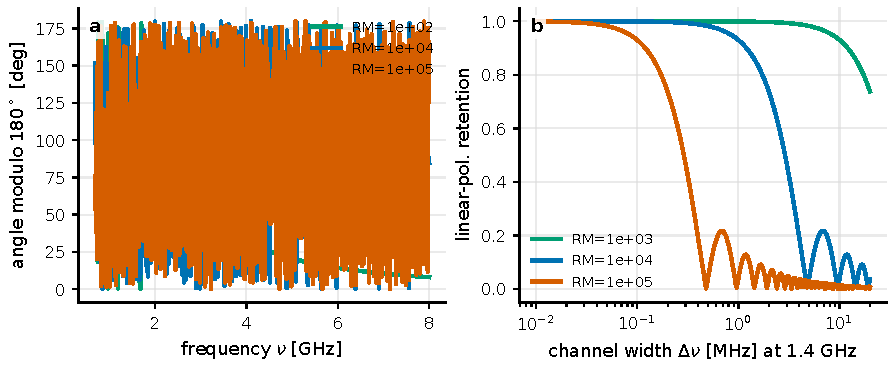
\includegraphics[width=0.94\linewidth]{figures/generated/chapter_15/ch15_frb_faraday_foreground.pdf}
\caption{FRB 偏振前景可以轻易淹没小旋转信号。左图显示不同 RM 下偏振角随频率的模 \(180^\circ\) 缠绕；\({\rm RM}=10^5\,{\rm rad\,m^{-2}}\) 在 GHz 频段变化极快。右图显示 \(1.4\,{\rm GHz}\) 附近有限通道宽度造成的线偏振保留率，窄通道是测高 RM 的必要条件。}
\label{fig:ch15-frb-faraday}
\end{figure}

\Needspace{11\baselineskip}
黑洞超辐射把轻玻色场和偏振图像连在一起。Kerr 黑洞角速度为 \(\Omega_H\)，玻色模满足
\begin{equation}
  \omega < m\Omega_H
  \label{eq:ch15-superradiance-condition}
\end{equation}
\begin{formulaexplain}[公式 (15.13) 解读]
\(\omega\) 是玻色模频率，\(m\) 是方位量子数，\(\Omega_H\) 是 Kerr 黑洞视界角速度。满足不等式时，波从黑洞自转中抽取能量，形成超辐射增长。
\end{formulaexplain}
时可从黑洞自转中抽取能量。定义
\begin{equation}
  \alpha_G=\frac{GM_\bullet m_a}{\hbar c},
  \label{eq:ch15-alpha-g}
\end{equation}
\begin{formulaexplain}[公式 (15.14) 解读]
\(\alpha_G\) 是黑洞引力半径和轴子 Compton 波长的比值，\(M_\bullet\) 是黑洞质量。它决定玻色云是否和黑洞尺度匹配；\(\alpha_G\sim0.1-1\) 时增长通常最有效。
\end{formulaexplain}
当 \(\alpha_G\sim0.1-1\) 时，玻色 Compton 波长与黑洞尺度匹配，云增长最快。相应轴子质量为
\begin{equation}
  m_a
  \simeq
  1.34\times10^{-10}\,{\rm eV}\,
  \alpha_G
  \left(\frac{M_\odot}{M_\bullet}\right).
  \label{eq:ch15-bh-mass-window}
\end{equation}
\begin{formulaexplain}[公式 (15.15) 解读]
这条式子把黑洞质量 \(M_\bullet\) 映射到最敏感的轴子质量 \(m_a\)。黑洞越重，对应的轴子质量窗口越低；因此 Sgr A* 和 M87* 探测的是不同超轻质量区。
\end{formulaexplain}
对 Sgr A* 的 \(4.3\times10^6M_\odot\)，\(\alpha_G=0.4\) 对应 \(m_a\simeq1.2\times10^{-17}\,{\rm eV}\)；对 M87* 的 \(6.5\times10^9M_\odot\)，对应 \(8\times10^{-21}\,{\rm eV}\)。EHT 偏振图像中的 axion cloud 模型预言，偏振角可随轴子周期振荡：Sgr A* 的周期可为 \(100-1000\,{\rm s}\)，M87* 可为数天，空间分辨率会决定这种振荡是否被环上不同方位平均掉 \citep{2015LNP...906.....B,2015CQGra..32m4001B,2017PhRvD..96c5019B,2020PhRvL.124f1102C,2022NatAs...6..592C}。

\begin{figure}[tbp]
\centering
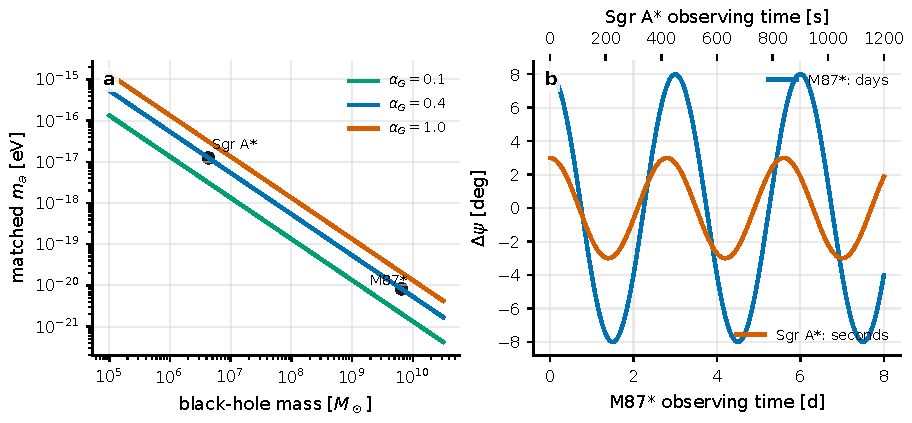
\includegraphics[width=0.94\linewidth]{figures/generated/chapter_15/ch15_black_hole_axion_cloud.pdf}
\caption{黑洞质量把超辐射轴子质量窗口定出来。左图用 \(\alpha_G=GM_\bullet m_a/\hbar c\) 标出不同黑洞质量对应的 \(m_a\)；Sgr A* 和 M87* 落在不同超轻质量区。右图画出 EHT 偏振角振荡的两个典型时间尺度：M87* 可在天尺度采样，Sgr A* 则需要秒到分钟级偏振成像。}
\label{fig:ch15-bh-axion}
\end{figure}

\section{暗物质小尺度透镜怎样把质量变成角偏移}

偏振检验寻找的是场对光子的量子通道影响；小尺度透镜检验寻找的是暗物质质量分布对光线路径的影响。两者共同点是信号常常不表现为“看到一团暗物质”，而表现为某个可观测量偏离普通模型。对透镜来说，这个可观测量可以是像位置、放大率、时间延迟或背景源的天体测量漂移。

暗物质存在本身可由星系团碰撞、弱透镜和动力学多种证据支持；Bullet Cluster 是经典例子，弱透镜质量峰与 X-ray 气体分离，表明主要质量成分近似无碰撞 \citep{2006ApJ...648L.109C,1993ApJ...404..441K}。小尺度结构给出另一类检验。CDM 数值模拟预言银河 halo 中有大量子晕和潮汐流，质量函数可延伸到远低于可见卫星星系的范围；Moore、Diemand 等结果使“暗的子结构”成为强透镜异常的重要候选解释 \citep{1994ApJ...427L...1F,1999ApJ...524L..19M,2008Natur.454..735D}。

子结构透镜的基本量级来自 Einstein 角
\begin{equation}
  \theta_E
  =
  \left(
  \frac{4GM}{c^2}
  \frac{D_{ls}}{D_lD_s}
  \right)^{1/2}.
  \label{eq:ch15-subhalo-einstein}
\end{equation}
\begin{formulaexplain}[公式 (15.16) 解读]
\(\theta_E\) 是子晕 Einstein 角，\(M\) 是透镜质量，距离组合给出几何效率。质量越大，角尺度按 \(M^{1/2}\) 增长；这直接决定强透镜异常需要的角分辨率。
\end{formulaexplain}
对 \(D_l\simeq1\,{\rm Gpc}\)、\(D_s\simeq2\,{\rm Gpc}\) 的星系强透镜，\(10^8M_\odot\) 子晕的 \(\theta_E\) 是几十 mas 量级，\(10^6M_\odot\) 则是几 mas。若像与子晕角距离为 \(b\gg\theta_E\)，点质量近似的天体测量偏移量为
\begin{equation}
  \delta\theta\simeq\frac{\theta_E^2}{b}.
  \label{eq:ch15-astrometric-shift}
\end{equation}
\begin{formulaexplain}[公式 (15.17) 解读]
\(\delta\theta\) 是天体测量偏移，\(b\) 是像到子晕的角距离。子晕越接近像、\(\theta_E\) 越大，位置扰动越明显；远离时信号按 \(1/b\) 变小。
\end{formulaexplain}
这个数量级把分辨率要求摆得很清楚：\(10^6M_\odot\) 子晕在 \(b=10\,{\rm mas}\) 处只给 \(\mu{\rm as}\) 量级偏移。强透镜 flux-ratio anomalies 对放大率扰动敏感，Mao 与 Schneider 指出低质量子结构可解释一些四像系统的异常；Dalal 与 Kochanek 用 7 个 radio lens 得到子结构质量分数中位数 \(f_{\rm sat}\simeq0.02\)，90\% 范围约 \(0.006-0.07\)；Vegetti 和 Hezaveh 等用 gravitational imaging 和 ALMA 数据把单个暗子结构探测推进到空间分辨建模 \citep{1998MNRAS.295..587M,2002ApJ...572...25D,2010MNRAS.408.1969V,2016ApJ...823...37H}。

\begin{figure}[tbp]
\centering
\includegraphics[width=0.94\linewidth]{figures/generated/chapter_15/ch15_dark_matter_lensing.pdf}
\caption{暗物质子晕的透镜信号受角尺度限制。左图给出典型 Gpc 几何下子晕 Einstein 角随质量的变化。右图把 \(\delta\theta\simeq\theta_E^2/b\) 转换为天体测量偏移；低质量子晕需要 mas 级接近和 \(\mu{\rm as}\) 级系统控制才容易看见。}
\label{fig:ch15-dm-lensing}
\end{figure}

Gaia 和未来天体测量巡天把这个问题变成时间域：子晕横穿背景源附近时，位置偏移随时间变化。若子晕横向速度 \(v_\perp\sim200\,{\rm km\,s^{-1}}\)，在 kpc 距离上对应 mas/yr 量级角速度；信号形状由 impact parameter、质量剖面和源自身 proper motion 共同决定。Mondino 等用 Gaia DR3 和未来 catalogues 讨论了这种 astrometric weak lensing 搜索，主要限制来自扫描定律、源密度、proper-motion covariance 和太阳系/仪器系统误差 \citep{2024MNRAS.531..632M}。PBH 暗物质也可通过透镜和动力学被限制，但质量函数、聚团和天体物理前景会改变解释 \citep{2016PhRvD..94h3504C}。

\section{怎样把异常写成可反驳的检验}

到这里为止，所有候选信号都有一个共同教训：异常本身不是结论，异常的可反驳结构才是结论。新物理搜索的观测量通常不止一个：偏振角、到达时间、像位置和放大率可能来自不同仪器，也有不同的统计误差和系统误差。把这些量合并为数据向量 \({\bf d}\) 后，模型可以分成
\begin{equation}
  {\bf m}({\boldsymbol\theta})
  =
  {\bf m}_{\rm src}
  +{\bf m}_{\rm prop}
  +{\bf m}_{\rm inst}
  +{\bf m}_{\rm new}({\boldsymbol\theta}),
  \label{eq:ch15-model-vector}
\end{equation}
\begin{formulaexplain}[公式 (15.18) 解读]
\({\bf m}\) 是模型预测向量，被拆成源、传播、仪器和新物理四项。这样的拆分强迫我们把异常先和普通天体物理、传播前景、校准误差放在同一个账本里比较。
\end{formulaexplain}
其中 \({\boldsymbol\theta}\) 包含 \(g_{a\gamma}\)、\(m_a\)、\(\beta\)、子晕质量函数或 PBH fraction 等参数。高斯近似下
\begin{equation}
  -2\ln\mathcal L
  =
  \left[{\bf d}-{\bf m}({\boldsymbol\theta})\right]^{\mathsf T}
  \left(C_{\rm stat}+C_{\rm sys}\right)^{-1}
  \left[{\bf d}-{\bf m}({\boldsymbol\theta})\right]
  +\ln\det(C_{\rm stat}+C_{\rm sys}).
  \label{eq:ch15-systematics-likelihood}
\end{equation}
\begin{formulaexplain}[公式 (15.19) 解读]
\(\mathcal L\) 是高斯似然，\(C_{\rm stat}\) 是统计协方差，\(C_{\rm sys}\) 是系统误差协方差。残差必须用两类误差共同加权；若漏掉系统项，单个异常会被错误地放大。
\end{formulaexplain}
\(C_{\rm stat}\) 来自 photon noise、TOA uncertainties 或图像噪声；\(C_{\rm sys}\) 包含 Mueller 矩阵、绝对偏振角、Faraday 前景、尘埃 EB、透镜宏模型、源结构和选择函数。若 \(C_{\rm sys}\) 未进入似然，单个异常点会被过度解释。

这些信号有清楚的相互区分方式。Faraday 旋转随 \(\lambda^2\) 变，轴子背景旋转近似 achromatic；静态 cosmic birefringence 在 CMB 中产生全局 EB/TB，超轻暗物质会在观测时间上振荡；黑洞轴子云应与黑洞质量、spin、环上方位和观测时间相关；暗物质子晕透镜应同时扰动像位置、放大率和时间延迟，而恒星表面结构主要随源旋转、波长和基线方向变化。可信结果通常要经受样本统计、空场或控制源、频率反演、时间相干性和仪器重标定的交叉检查。

CMB 和早期宇宙涨落把同一要求推到全天图层面。那里的观测对象不再是单个源的偏振角或透镜像，而是 \(T/E/B\) 图、功率谱、偏振角和系统误差矩阵。


\chapter{宇宙学中的量子问题}
\label{chap:16}

\begin{chapteropening}
CMB 是最接近“整个宇宙作为光学实验”的观测对象，但它不是实验室里可以反复制备的量子光源。观测者得到的是一张带频率、偏振、角位置和噪声权重的天空图，再从图中估计角功率谱、相关函数、非高斯性和偏振旋转。量子语言出现在初始涨落、暴胀中的模式放大、两模压缩和退相干；数据语言则是 \(\mu{\rm K}\) 级温度涨落、\(E/B\) 偏振、\(C_\ell\)、\(f_{\rm NL}\)、张量标量比 \(r\) 和系统误差矩阵。COBE/FIRAS、COBE/DMR、WMAP/Planck、BICEP/Keck 和 CMB 偏振双折射分析给出了这些量的观测尺度 \citep{1967PhRvL..19.1199S,1990ApJ...354L..37M,1992ApJ...396L...1S,1994ApJ...420..439M,1996ApJ...473..576F,2009ApJ...707..916F,2020A&A...641A...1P,2020A&A...641A...5P,2020A&A...641A...6P,2020A&A...641A..10P,2021PhRvL.127o1301A}。
\end{chapteropening}

\section{CMB 首先是什么样的光场}

CMB 常被直接拿来谈暴胀量子涨落，但观测入口其实很朴素：望远镜先看到一个几乎完美黑体的微波天空，然后在这个平均背景上测 \(10^{-5}\) 量级的角向涨落和更弱的偏振结构。因此本章先从光场本身开始，再逐步退回到产生这些统计图样的早期量子模式。

平均 CMB 近似为温度
\[
  T_0 = 2.7255\pm0.0006\,{\rm K}
\]
的黑体。Planck 分布给出每个频率模式的平均光子占据数和比强度
\begin{equation}
  n_\nu
  =
  \frac{1}{\exp(h\nu/k_{\rm B}T_0)-1},
  \qquad
  I_\nu
  =
  \frac{2h\nu^3}{c^2}n_\nu .
  \label{eq:ch16-planck-spectrum}
\end{equation}
\begin{formulaexplain}[公式 (16.1) 解读]
\(n_\nu\) 是单个频率模式的平均光子数，\(I_\nu\) 是黑体比强度，\(T_0\) 是 CMB 平均温度。低频时 \(n_\nu\) 大，场更接近经典热光；高频时单模占据数下降，但总探测光子数仍由带宽和光束面积决定。
\end{formulaexplain}
\(\nu\) 用 Hz，\(I_\nu\) 的单位是 \({\rm erg\,s^{-1}\,cm^{-2}\,Hz^{-1}\,sr^{-1}}\)，CMB 文献常换成 \({\rm MJy\,sr^{-1}}\)。在 \(30\,{\rm GHz}\)，\(h\nu/k_{\rm B}T_0\simeq0.53\)，\(n_\nu\sim1.4\)，低频通道仍接近经典热场；在 \(150\,{\rm GHz}\)，\(n_\nu\simeq0.07\)，单模占据数已小于 1，但总光子数因望远镜带宽和角分辨元巨大而很高。黑体强度峰在 \(160\,{\rm GHz}\) 附近，这是 Planck HFI 和许多地面 CMB 实验选择 \(90/150/220\,{\rm GHz}\) 通道的物理背景。FIRAS 对黑体谱的精度把早期能量注入、谱畸变和非热辐射限制到极小水平，因此现代 CMB 宇宙学通常把平均谱当作已知背景，把信息放在角向涨落和偏振上 \citep{1994ApJ...420..439M,1996ApJ...473..576F,2009ApJ...707..916F}。

\begin{figure}[tbp]
\centering
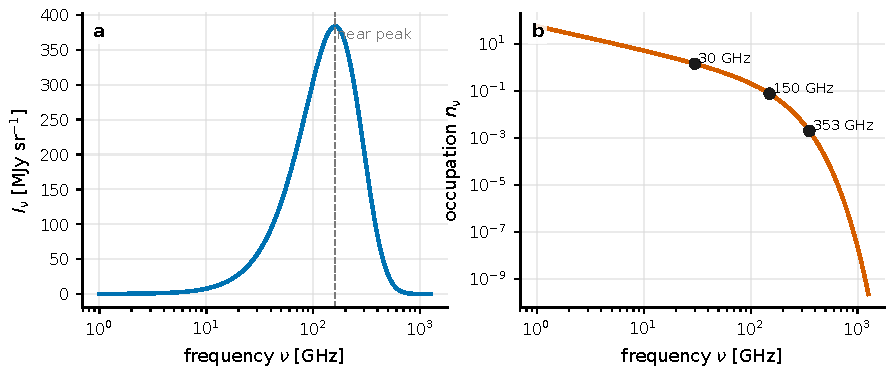
\includegraphics[width=0.94\linewidth]{figures/generated/chapter_16/ch16_cmb_blackbody.pdf}
\caption{CMB 的平均光场由黑体谱和模式占据数共同决定。左图把 \(T_0=2.7255\,{\rm K}\) 的 Planck 谱写成 \({\rm MJy\,sr^{-1}}\)，峰值在 \(160\,{\rm GHz}\) 附近。右图显示同一黑体在不同频率的单模平均光子数；低频通道占据数较高，高频通道逐渐进入 \(n_\nu<1\) 的量级。}
\label{fig:ch16-cmb-blackbody}
\end{figure}

角向涨落写成
\begin{equation}
  T(\hat{\bf n})
  =
  T_0\,[1+\Theta(\hat{\bf n})],
  \qquad
  \Theta(\hat{\bf n})
  =
  \sum_{\ell m}a_{\ell m}^{T}Y_{\ell m}(\hat{\bf n}).
  \label{eq:ch16-temperature-expansion}
\end{equation}
\begin{formulaexplain}[公式 (16.2) 解读]
\(\Theta(\hat{\bf n})\) 是无量纲温度涨落，\(a_{\ell m}^{T}\) 是球谐系数，\(Y_{\ell m}\) 是球谐函数。这条式子把一张天空图拆成角尺度模式：\(\ell\) 控制尺度，\(m\) 控制同一尺度上的方位自由度。
\end{formulaexplain}
\(\hat{\bf n}\) 是天空方向，\(a_{\ell m}^T\) 是无量纲温度涨落系数；实际图上常把 \(T_0\Theta\) 写成 \(\mu{\rm K}\)。COBE/DMR 首次在全天图上看到 \(\Delta T/T\sim10^{-5}\) 的结构，现代 Planck 地图把这个信号分解到 \(\ell\sim2500\) 量级。多极矩 \(\ell\) 与角尺度近似满足 \(\theta\simeq180^\circ/\ell\)：\(\ell\simeq2\) 对应半个天空，\(\ell\simeq200\) 对应一度角，\(\ell\simeq2000\) 对应几角分。各向同性高斯天空的角功率谱估计量为
\begin{equation}
  \widehat C_\ell^{TT}
  =
  \frac{1}{2\ell+1}
  \sum_{m=-\ell}^{\ell}
  |a_{\ell m}^{T}|^2,
  \qquad
  D_\ell^{TT}
  =
  \frac{\ell(\ell+1)}{2\pi}C_\ell^{TT}.
  \label{eq:ch16-cl-estimator}
\end{equation}
\begin{formulaexplain}[公式 (16.3) 解读]
\(\widehat C_\ell^{TT}\) 是温度角功率谱估计量，来自同一 \(\ell\) 上所有 \(m\) 模式的平均；\(D_\ell\) 是常用的重标度形式。这个平均就是 CMB 二点统计的核心压缩。
\end{formulaexplain}
\(C_\ell\) 的单位取决于 \(a_{\ell m}\) 是否乘了温度；若 \(a_{\ell m}\) 用 \(\mu{\rm K}\)，\(C_\ell\) 和 \(D_\ell\) 就是 \(\mu{\rm K}^2\)。\(D_\ell^{TT}\) 第一声学峰位于 \(\ell\simeq220\)，峰高约 \(5\times10^3\,\mu{\rm K}^2\)。这些峰来自光子-重子流体在复合前的声学振荡：重子密度改变压缩峰高度，暗物质密度改变引力势衰减，角直径距离把物理声学尺度投影成角尺度。Planck 2018 在六参数平直 \(\Lambda{\rm CDM}\) 中给出 \(\Omega_bh^2=0.0224\)、\(\Omega_ch^2=0.120\)、\(n_s=0.965\)、\(\tau=0.054\)、\(H_0=67.4\,{\rm km\,s^{-1}\,Mpc^{-1}}\)、\(\Omega_m=0.315\)、\(\sigma_8=0.811\) 的典型精度 \citep{1992ApJ...396L...1S,1996ApJ...469..437S,2020A&A...641A...5P,2020A&A...641A...6P,2021A&A...652C...4P}。

即使没有仪器噪声，全天也只给每个 \(\ell\) 的 \(2\ell+1\) 个 \(m\) 模式。高斯天空的 cosmic variance 为
\begin{equation}
  \frac{\sigma(C_\ell)}{C_\ell}
  =
  \sqrt{\frac{2}{(2\ell+1)f_{\rm sky}}},
  \label{eq:ch16-cosmic-variance}
\end{equation}
\begin{formulaexplain}[公式 (16.4) 解读]
\(\sigma(C_\ell)/C_\ell\) 是样本方差的相对误差，\(f_{\rm sky}\) 是有效天区比例。低 \(\ell\) 可用模式少，所以即使仪器完美，大角尺度也有无法消除的统计不确定性。
\end{formulaexplain}
\(f_{\rm sky}\) 是有效天空覆盖率。全天 \(\ell=2\) 的相对误差约 \(63\%\)，\(\ell=200\) 降到 \(7\%\)，\(\ell=2000\) 约 \(2.2\%\)；若银河面和强前景区被 mask，\(f_{\rm sky}<1\)，误差还会增大。因此低 \(\ell\) 异常、四极矩偏低或 hemispherical asymmetry 要放进有限模式数的协方差中，而不宜只凭单个点在图上的显眼程度判断。

\begin{figure}[tbp]
\centering
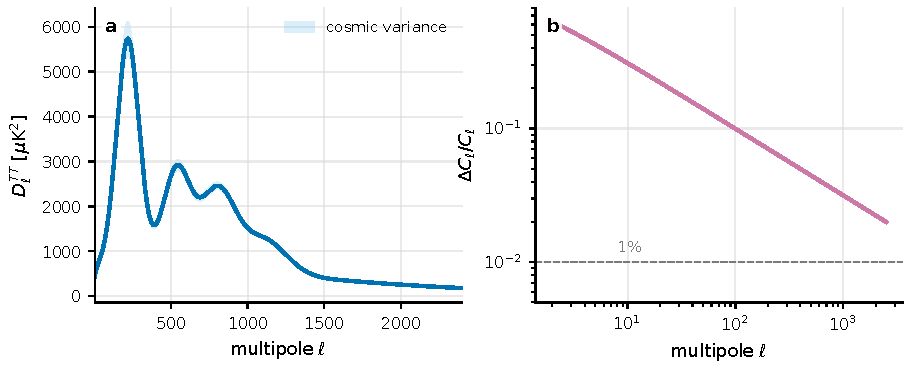
\includegraphics[width=0.94\linewidth]{figures/generated/chapter_16/ch16_cmb_power_spectrum.pdf}
\caption{角功率谱把天空涨落压缩到多极矩空间。左图是带声学峰和阻尼尾的标度图，蓝色阴影表示全天 cosmic variance 的量级；右图单独画出 \(\sqrt{2/(2\ell+1)}\)，显示大角尺度的误差由天空上可用模式数限制，望远镜灵敏度无法消除这部分方差。}
\label{fig:ch16-cmb-power}
\end{figure}

偏振图比温度图多两个 Stokes 参数。把 \(Q\) 和 \(U\) 组成 spin-2 场后，
\begin{equation}
  (Q\pm iU)(\hat{\bf n})
  =
  \sum_{\ell m}
  a_{\pm2,\ell m}\,{}_{\pm2}Y_{\ell m}(\hat{\bf n}),
  \qquad
  a_{\ell m}^{E}
  =
  -\frac{1}{2}(a_{2,\ell m}+a_{-2,\ell m}),
  \quad
  a_{\ell m}^{B}
  =
  \frac{i}{2}(a_{2,\ell m}-a_{-2,\ell m}).
  \label{eq:ch16-eb-definition}
\end{equation}
\begin{formulaexplain}[公式 (16.5) 解读]
\(Q\pm iU\) 是自旋 \(\pm2\) 的偏振场，\({}_{\pm2}Y_{\ell m}\) 是自旋球谐函数，\(a_{\ell m}^{E/B}\) 是 E/B 模系数。这个分解把局部偏振方向转换成全天天空上的标量型和旋量型图样。
\end{formulaexplain}
\(E\) 模在宇称变换下像标量，\(B\) 模像赝标量。标量密度涨落在线性阶主要产生 \(T\) 和 \(E\)，不直接产生原初 \(B\)；张量扰动、弱透镜、偏振角旋转、银河尘埃和同步辐射都能产生 \(B\)。因此，B 模检出需要和频率分离、delensing、角标定和 foreground model 一起解释，才能指向原初引力波。E/B 分解的全天天空形式来自 Zaldarriaga-Seljak 和 Kamionkowski-Kosowsky-Stebbins 的经典工作；后来的 BICEP/Keck 约束把这个数学分解变成了原初引力波搜索的主要观测通道 \citep{1997PhRvD..55.1830Z,1997PhRvL..78.2054S,1997PhRvL..78.2058K,2021PhRvL.127o1301A}。

\section{暴胀涨落为什么像两模压缩态}

上一节的 \(C_\ell\) 是天空上的统计量；暴胀理论要解释的是这些统计量为什么有近似高斯性、近似尺度不变性和固定声学相位。这里不能把 CMB 当成一束可反复制备的实验室光，而要把早期宇宙中的场模式当成时变谐振子。暴胀量子涨落通常不用单个光子的语言写，而是写成规范不变量的场模式。对标量曲率扰动 \(\mathcal R\)，定义 Mukhanov-Sasaki 变量
\begin{equation}
  v({\bf x},\eta)=z(\eta)\mathcal R({\bf x},\eta),
  \qquad
  z=\frac{a\dot\phi}{H},
  \label{eq:ch16-ms-variable}
\end{equation}
\begin{formulaexplain}[公式 (16.6) 解读]
\(v\) 是 Mukhanov-Sasaki 变量，\(\mathcal R\) 是曲率扰动，\(z=a\dot\phi/H\) 包含背景暴胀演化。用 \(v\) 写方程，可以把每个 Fourier 模看成一个时变频率的量子谐振子。
\end{formulaexplain}
\(\eta\) 是 conformal time，\(a\) 是尺度因子，\(\phi\) 是驱动暴胀的背景场，\(H=\dot a/a\)。在二阶作用量中，每个 Fourier 模近似是时变频率谐振子：
\begin{equation}
  v_k''+
  \left(k^2-\frac{z''}{z}\right)v_k
  =
  0 .
  \label{eq:ch16-ms-equation}
\end{equation}
\begin{formulaexplain}[公式 (16.7) 解读]
\(v_k\) 是共动波数 \(k\) 的模式函数，\(z''/z\) 是背景膨胀给出的有效势。亚视界时 \(k^2\) 主导，模式像真空振子；出视界后有效势主导，曲率扰动幅度被冻结。
\end{formulaexplain}
\(k\) 是共动波数，单位常用 \({\rm Mpc^{-1}}\)；撇号是对 \(\eta\) 求导。亚视界时 \(k\gg aH\)，方程近似 \(v_k''+k^2v_k=0\)，Bunch-Davies 真空取
\[
  v_k\simeq \frac{e^{-ik\eta}}{\sqrt{2k}}.
\]
当 \(k\simeq aH\) 穿出视界后，\(z''/z\) 项主导，增长解被冻结，衰减解迅速变小，\(\mathcal R_k=v_k/z\) 变成近似常数。这里的“冻结”指相位空间中一个象限被强烈压窄，最后只剩一个随机幅度控制后来的密度扰动；它并不表示模式完全停止演化 \citep{1988JETP...67.1297M,1990PhRvD..42.3413G,1996CQGra..13..377P}。

功率谱定义为
\begin{equation}
  \langle
  \mathcal R_{\bf k}\mathcal R_{{\bf k}'}
  \rangle
  =
  (2\pi)^3\delta^{(3)}({\bf k}+{\bf k}')
  \frac{2\pi^2}{k^3}
  \mathcal P_{\mathcal R}(k),
  \qquad
  \mathcal P_{\mathcal R}(k)
  =
  A_s
  \left(\frac{k}{k_*}\right)^{n_s-1}.
  \label{eq:ch16-primordial-spectrum}
\end{equation}
\begin{formulaexplain}[公式 (16.8) 解读]
\(\mathcal P_{\mathcal R}(k)\) 是无量纲原初曲率功率谱，\(A_s\) 是振幅，\(n_s\) 是谱指数，\(k_*\) 是 pivot。它把早期量子涨落的二点统计写成今天 CMB 拟合的核心参数。
\end{formulaexplain}
\(A_s\) 是无量纲振幅，Planck 常用 pivot \(k_*=0.05\,{\rm Mpc^{-1}}\)，并给出 \(\ln(10^{10}A_s)\simeq3.04\)，即 \(A_s\simeq2.1\times10^{-9}\)。\(n_s=1\) 是精确 scale-invariant；Planck 的 \(n_s\simeq0.965\) 表示红倾，长波模式略强。这个 \(10^{-9}\) 的原初曲率功率经过辐射转移函数、重子声学振荡、复合面厚度、透镜和平滑，投影成今天 \(\Delta T/T\sim10^{-5}\) 的天空涨落 \citep{2020A&A...641A...6P,2020A&A...641A..10P}。

在量子光学语言里，暴胀把 \({\bf k}\) 和 \(-{\bf k}\) 两个模式从真空演化成两模压缩态，
\begin{equation}
  |\psi\rangle
  =
  \prod_{\bf k}
  \exp\!\left[
    r_k e^{-2i\varphi_k}a_{\bf k}a_{-{\bf k}}
    -
    r_k e^{2i\varphi_k}a_{\bf k}^\dagger a_{-{\bf k}}^\dagger
  \right]
  |0\rangle .
  \label{eq:ch16-squeezed-state}
\end{equation}
\begin{formulaexplain}[公式 (16.9) 解读]
\(|\psi\rangle\) 是 \({\bf k}\) 与 \(-{\bf k}\) 成对的两模压缩态，\(r_k\) 是压缩强度，\(\varphi_k\) 是压缩角。暴胀的时变背景把真空涨落成对放大，并保留固定相位关系。
\end{formulaexplain}
\(r_k\) 是 squeezing parameter，\(\varphi_k\) 是 squeezing angle。平均占据数 \(N_k=\sinh^2r_k\)；超视界很久以后 \(r_k\) 很大，\(N_k\) 可指数增大。这里的“占据数”指早期场模式的量子激发数，和望远镜实际数到的 CMB 光子数不是同一个量。对经历 \(50-60\) 个 e-folds 后重新进入视界的模式，衰减象限已经极小，Wigner 函数像一条细长椭圆，后来的声学振荡继承了固定相位。这种固定相位解释了 CMB \(TT\)、\(TE\)、\(EE\) 谱中成串声学峰，而不是一团随机相位波纹 \citep{1990PhRvD..42.3413G,1996CQGra..13..377P,2006CQGra..23.2317P}。

\begin{figure}[tbp]
\centering
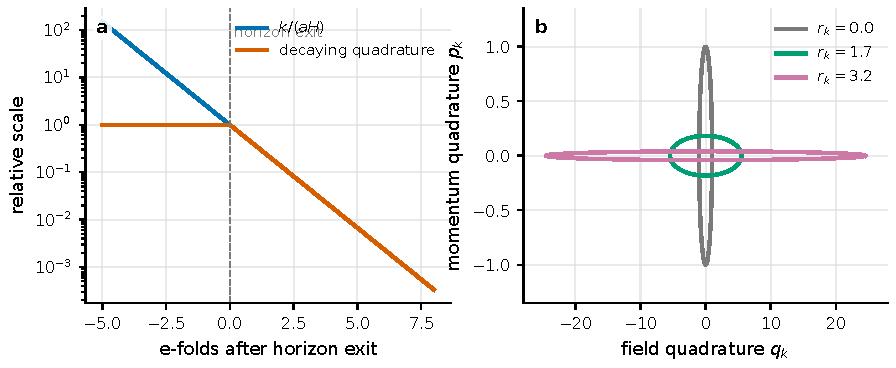
\includegraphics[width=0.94\linewidth]{figures/generated/chapter_16/ch16_squeezed_modes.pdf}
\caption{暴胀中的模式放大可以看成两模压缩。左图显示 \(k/(aH)\) 在穿出视界后指数下降，同时衰减象限被压小。右图画相空间椭圆：\(r_k\) 增大时，一个象限被拉长，另一个象限被压窄；观测到的是后来表现为经典随机幅度的长轴信息。}
\label{fig:ch16-squeezed}
\end{figure}

退相干把“纯压缩态”变成可用经典随机场描述的有效状态。这里的环境可以是未观测短波模式、张量/标量相互作用、复合前等离子体自由度、透镜势或数据处理中被 marginalize 掉的前景和仪器模式。写成密度矩阵时，观测变量 \(q_k\) 的有效约化矩阵近似为
\begin{equation}
  \rho_{\rm red}(q,q')
  =
  \rho_0(q,q')
  \exp\!\left[-\Gamma_k(q-q')^2\right],
  \label{eq:ch16-decoherence-density}
\end{equation}
\begin{formulaexplain}[公式 (16.10) 解读]
\(\rho_{\rm red}\) 是观测变量的约化密度矩阵，\(\rho_0\) 是未退相干形式，\(\Gamma_k\) 衡量环境抑制非对角项的强度。当 \(q\neq q'\) 的相干项被压低后，功率谱可用经典随机场语言计算。
\end{formulaexplain}
\(\Gamma_k\) 是退相干强度，单位取决于 \(q_k\) 的归一化。若 \(\Gamma_k(\Delta q)^2\gg1\)，不同幅度分支之间的干涉项被压低，功率谱和相关函数可按经典随机场计算。早期宇宙的“测量问题”仍有概念层面的争论；但对 \(C_\ell\)、\(B_\ell\) 和 lensing reconstruction 这些观测量而言，保留下来的相干相位信息不足以表现为实验室式 Bell 测试或可反复制备的非经典态 \citep{1996CQGra..13..377P,2006CQGra..23.2317P}。

\section{非高斯性和张量模式分别检验什么}

二点函数告诉我们“有多少涨落”；更高点函数和张量模式则问“这些涨落怎样产生”。非高斯性检验暴胀期间的相互作用和场内容，张量 B 模检验是否存在原初引力波背景。两者都很诱人，也都非常容易被有限模式数、透镜、尘埃和模板选择限制。

若 \(\mathcal R\) 是严格高斯场，所有信息都在二点函数中；三点函数和更高点函数为零。暴胀相互作用、非平凡声速、多场转移、激发初态或尖锐特征会产生非高斯性。三点函数写成
\begin{equation}
  \langle
  \mathcal R_{{\bf k}_1}
  \mathcal R_{{\bf k}_2}
  \mathcal R_{{\bf k}_3}
  \rangle
  =
  (2\pi)^3
  \delta^{(3)}({\bf k}_1+{\bf k}_2+{\bf k}_3)
  B_{\mathcal R}(k_1,k_2,k_3).
  \label{eq:ch16-bispectrum}
\end{equation}
\begin{formulaexplain}[公式 (16.11) 解读]
\(B_{\mathcal R}\) 是曲率扰动的 bispectrum，三个 \(k\) 必须由 delta 函数闭合成三角形。不同三角形形状对应不同早期宇宙相互作用，因此三点函数是非高斯性的主要语言。
\end{formulaexplain}
\(B_{\mathcal R}\) 的三个 \(k\) 构成一个三角形。local 型在 squeezed triangle 中最强，即 \(k_1\ll k_2\simeq k_3\)；equilateral 型在三边相等时最强；orthogonal 型是为区分不同相互作用而构造的近似正交模板。local ansatz 常写成
\begin{equation}
  \mathcal R({\bf x})
  =
  \mathcal R_g({\bf x})
  +
  \frac{3}{5}f_{\rm NL}^{\rm local}
  \left[
    \mathcal R_g^2({\bf x})
    -
    \langle\mathcal R_g^2\rangle
  \right],
  \label{eq:ch16-local-fnl}
\end{equation}
\begin{formulaexplain}[公式 (16.12) 解读]
\(\mathcal R_g\) 是高斯场，\(f_{\rm NL}^{\rm local}\) 是 local 型非高斯振幅。二次项让长波模式调制短波功率，因此 local 模板在 squeezed 构型中最敏感。
\end{formulaexplain}
\(\mathcal R_g\) 是高斯部分，\(f_{\rm NL}\) 无量纲。Planck 2018 的温度加偏振结果给出 \(f_{\rm NL}^{\rm local}=-0.9\pm5.1\)、\(f_{\rm NL}^{\rm equil}=-26\pm47\)、\(f_{\rm NL}^{\rm orth}=-38\pm24\) 的 \(68\%\) C.L. 约束，没有发现标准模板的显著非高斯性。单场慢滚暴胀的 squeezed-limit consistency relation 预言 local 非高斯很小，数量级与 \(1-n_s\) 相近；Maldacena 的三阶作用量计算是这个结论的标准来源 \citep{2003JHEP...05..013M,2020A&A...641A...9P,2020A&A...641A..10P}。

\begin{figure}[tbp]
\centering
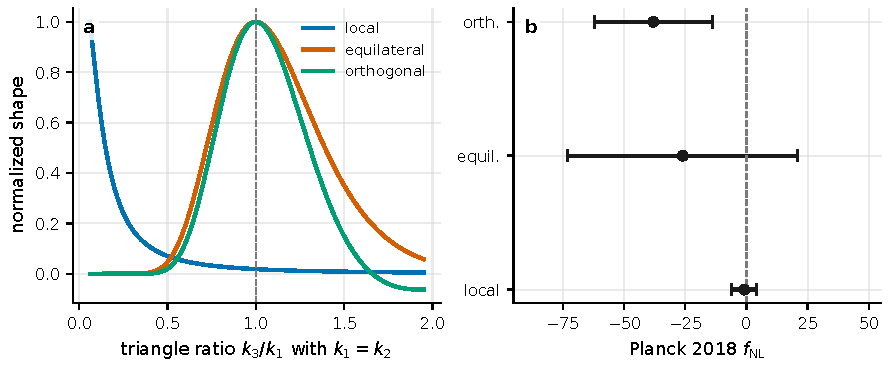
\includegraphics[width=0.94\linewidth]{figures/generated/chapter_16/ch16_non_gaussian_templates.pdf}
\caption{非高斯性由三角形构型和振幅共同决定。左图用 \(k_1=k_2\) 的切片比较 local、equilateral 和 orthogonal 模板的形状；local 型在 squeezed 极限增强，equilateral 型在三边接近相等时最大。右图给出 Planck 2018 对三个常用 \(f_{\rm NL}\) 参数的代表性约束，误差条均与零相容。}
\label{fig:ch16-nongaussian}
\end{figure}

张量扰动是量子引力背景最直接的 CMB 目标。定义
\begin{equation}
  r(k_*)=
  \frac{\mathcal P_t(k_*)}{\mathcal P_{\mathcal R}(k_*)},
  \qquad
  \mathcal P_t(k)
  =
  A_t\left(\frac{k}{k_*}\right)^{n_t}.
  \label{eq:ch16-tensor-r}
\end{equation}
\begin{formulaexplain}[公式 (16.13) 解读]
\(r\) 是张量功率谱和标量曲率功率谱在 pivot \(k_*\) 处的比值，\(\mathcal P_t\) 用振幅 \(A_t\) 和 tilt \(n_t\) 描述。它把原初引力波背景压缩成 CMB B 模搜索最常引用的参数。
\end{formulaexplain}
\(r\) 无量纲，pivot 常取 \(0.002\) 或 \(0.05\,{\rm Mpc^{-1}}\)，不同下标不能混用。单场慢滚给出近似 consistency relation \(n_t\simeq-r/8\)。若把 \(r\) 转成暴胀能标，
\begin{equation}
  V_*^{1/4}
  \simeq
  1.06\times10^{16}\,{\rm GeV}
  \left(\frac{r}{0.01}\right)^{1/4},
  \label{eq:ch16-inflation-scale}
\end{equation}
\begin{formulaexplain}[公式 (16.14) 解读]
\(V_*^{1/4}\) 是暴胀能标，\(r\) 是张量标量比。因为四次方根关系，即使 \(r\) 的上限大幅改善，能标约束也只缓慢收紧。
\end{formulaexplain}
这里假设爱因斯坦引力、标准慢滚和单一能量标尺。Planck 2018 单独给出 \(r_{0.002}<0.10\) 的 \(95\%\) C.L. 上限；结合 BK15 B 模偏振得到 \(r_{0.002}<0.056\)，对应 \(V_*^{1/4}<1.6\times10^{16}\,{\rm GeV}\)。BICEP/Keck 2018 season 与 Planck、WMAP 联合分析给出 \(r_{0.05}<0.036\) 的 \(95\%\) C.L. 上限，并指出无 lensing 或无尘埃的理想模拟会显著降低 \(\sigma(r)\)；目前限制同时受 lensing B 模和银河尘埃影响 \citep{2020A&A...641A..10P,2021PhRvL.127o1301A,2019JCAP...02..056A}。

\begin{figure}[tbp]
\centering
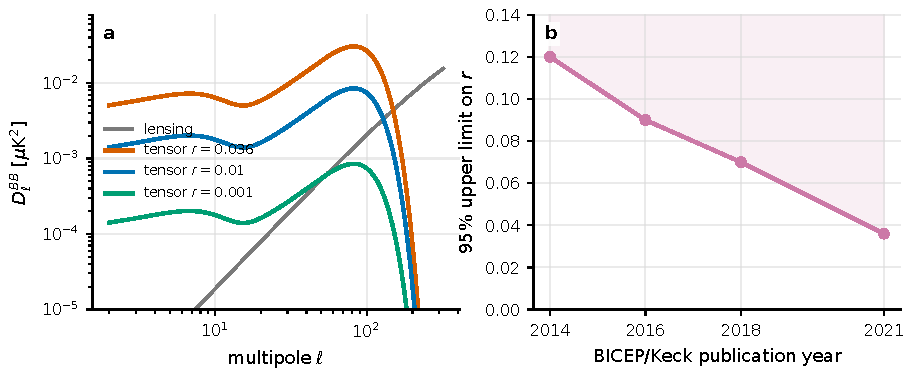
\includegraphics[width=0.94\linewidth]{figures/generated/chapter_16/ch16_bmode_constraints.pdf}
\caption{张量模式主要通过 B 模偏振受限。左图比较透镜 B 模和不同 \(r\) 的原初 tensor B 模标度；\(\ell\sim80\) 的 recombination bump 是地面实验的主战场，低 \(\ell\) reionization bump 需要大天区控制。右图显示 BICEP/Keck 系列联合约束从 \(r<0.12\) 改进到 \(r_{0.05}<0.036\) 的量级。}
\label{fig:ch16-bmode}
\end{figure}

\section{CMB 偏振双折射怎样区分宇宙角和仪器角}

第 \ref{chap:15} 章已经把轴子样场造成的偏振旋转写成 Stokes 量和 \(E/B\) 模混合，见式 \eqref{eq:ch15-qu-rotation} 和式 \eqref{eq:ch15-cmb-eb-tb}。放到 CMB 里，它首先变成一个校准问题：天空真的转过一个角，和仪器偏振角整体错一个角，在 \(EB/TB\) 统计中几乎同向。在 CMB 分析里，观测任务是把一个很小的全局角 \(\beta\) 从探测器角标定、银河尘埃、同步辐射和 map-making residual 中分出来。\(\beta\) 用弧度代入三角函数；\(0.35^\circ=6.1\times10^{-3}\,{\rm rad}\)，因此在小角度极限 \(EB/(EE-BB)\simeq2\beta\simeq1.2\%\)。这个百分之一信号足够大，可以在 Planck 级全天数据里留下统计迹象；也足够小，任何绝对偏振角标定、尘埃 EB、bandpass mismatch 或 beam leakage 都可能伪装它 \citep{2020PhRvL.125v1301M,2022PhRvD.106f3503E,2022PhRvL.128i1302D,2022NatRP...4..452K}。

\begin{figure}[tbp]
\centering
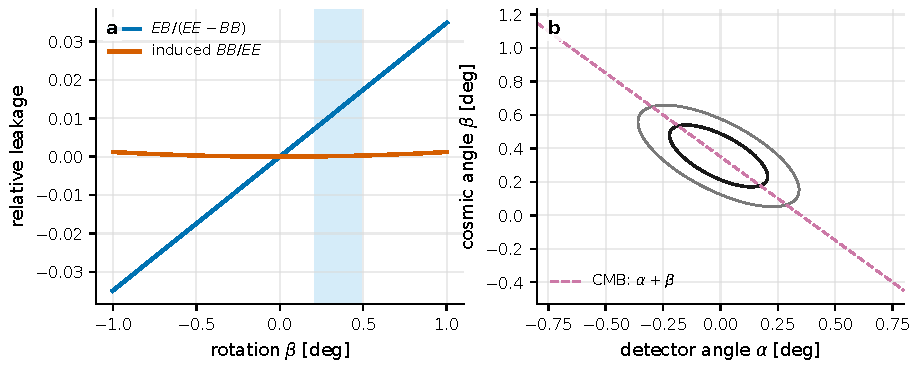
\includegraphics[width=0.94\linewidth]{figures/generated/chapter_16/ch16_birefringence_eb.pdf}
\caption{CMB 双折射把偏振角误差和宇宙学信号放在同一个平面里。左图显示 \(\beta\) 对 \(EB\) 和诱导 \(BB\) 的小角度泄漏；蓝色阴影标出 \(\beta=0.35\pm0.14^\circ\) 的量级。右图显示 detector angle \(\alpha\) 和 cosmic angle \(\beta\) 的退化方向：只用 CMB 时主要测到 \(\alpha+\beta\)，加入前景频率和多极矩信息才可能分离两者。}
\label{fig:ch16-birefringence}
\end{figure}

Minami 和 Komatsu 的 Planck 2018 分析利用 CMB 与银河前景偏振的不同频率依赖，同时估计 detector miscalibration \(\alpha_\nu\) 和 cosmic birefringence \(\beta\)，得到 \(\beta=0.35\pm0.14^\circ\)，并把地面角标定 \(0.28^\circ\) 的系统误差从最终误差中分离出去。后续 WMAP+Planck PR4 分析在 \(23-353\,{\rm GHz}\) 范围内加入 LFI/HFI 和 dust EB 模型，给出近全天 \(\beta=0.342^{+0.094}_{-0.091}{}^\circ\)，显著性约 \(3.6\sigma\)，但 polarized dust 的 intrinsic \(EB\)、低频 synchrotron EB 和独立角标定仍是主要限制。把这个信号解释成轴子样场时，旋转角来自
\begin{equation}
  \beta
  =
  \frac{1}{2}g_{\phi\gamma}
  [\phi(t_0)-\phi(t_{\rm LSS})],
  \label{eq:ch16-axion-birefringence}
\end{equation}
\begin{formulaexplain}[公式 (16.15) 解读]
\(\beta\) 是 CMB 偏振全局旋转角，\(g_{\phi\gamma}\) 是场-光子耦合，括号内是今天和最后散射面之间的场值差。若旋转来自轴子样传播效应，它应近似无频率依赖。
\end{formulaexplain}
\(g_{\phi\gamma}\) 的单位是 \({\rm GeV^{-1}}\)，\(\phi\) 是从最后散射面到今天的有效场值差。这个式子假设旋转近似各向同性、频率无关，并且源自传播过程而非发射面本征 \(EB\)。若 \(\beta(\nu)\propto\nu^{-2}\)，更像 Faraday 旋转；若 \(\beta\) 随天区、红移或时间变化，则需要从单个全局角推广到方向依赖或时间依赖的相关函数 \citep{2020PhRvL.125v1301M,2022PhRvL.128i1302D,2022NatRP...4..452K}。

\section{CMB 怎样与光学量子天文学对接}

CMB 和前几章的光学量子天文学共享“相关函数”语言，但观测含义不同。前几章更多处理可重复观测的源、可调的频带和可设计的探测链；CMB 则只有一片天空、一个初始条件和一套必须被充分建模的前景。这个差别决定了两边的“量子”不能简单互相替换。

实验室或恒星 HBT 中常用
\[
  g^{(2)}(\tau)
  =
  \frac{\langle I(t)I(t+\tau)\rangle}{\langle I\rangle^2}
\]
直接描述探测器时间序列中的强度涨落；CMB 的基本二点函数是天空球面上的
\begin{equation}
  \langle
  X_{\ell m}Y_{\ell' m'}^*
  \rangle
  =
  C_\ell^{XY}\delta_{\ell\ell'}\delta_{mm'},
  \qquad
  X,Y\in\{T,E,B,\phi_{\rm lens}\}.
  \label{eq:ch16-cmb-correlator}
\end{equation}
\begin{formulaexplain}[公式 (16.16) 解读]
\(C_\ell^{XY}\) 是两个天空场 \(X,Y\) 的角功率谱，Kronecker delta 表示在各向同性天空中不同 \(\ell,m\) 模式不相关。它是 CMB 版的二点相关函数语言。
\end{formulaexplain}
\(g^{(2)}\) 的时间延迟和带宽由仪器可主动选择；\(C_\ell\) 的模式数由宇宙给定，观测者只能改变 sky mask、频率组合、beam、noise weighting 和前景模型。CMB 无法像实验室系统那样调制源、重复制备初态或改变量子态；它提供的是早期场模式统计信息在 \(T/E/B\)、lensing 和 higher-order correlations 中的投影。

在 map-level 分析中，频率图、偏振图和外部 tracer 都进入同一个数据向量 \({\bf d}\)：
\begin{equation}
  {\bf d}
  =
  {\bf P}
  [
    {\bf s}_{\rm CMB}({\boldsymbol\theta})
    +
    {\bf s}_{\rm fg}({\boldsymbol\eta})
  ]
  +
  {\bf n},
  \qquad
  -2\ln\mathcal L
  =
  ({\bf d}-{\bf m})^{\mathsf T}
  C^{-1}
  ({\bf d}-{\bf m})
  +
  \ln\det C .
  \label{eq:ch16-cmb-likelihood}
\end{equation}
\begin{formulaexplain}[公式 (16.17) 解读]
\({\bf d}\) 是地图级数据向量，\({\bf P}\) 是观测和制图算子，\({\bf s}_{\rm CMB}\) 与 \({\bf s}_{\rm fg}\) 是宇宙信号和前景，\({\bf n}\) 是噪声。似然把模型残差和总协方差 \(C\) 放在一起，是从天空图推断宇宙学参数的工作形式。
\end{formulaexplain}
\({\bf P}\) 包含 beam、mask、scan strategy、bandpass 和 map-making；\({\boldsymbol\theta}\) 是宇宙学参数，例如 \(A_s,n_s,\Omega_bh^2,\Omega_ch^2,\tau,r,\beta\)；\({\boldsymbol\eta}\) 是前景参数，例如尘埃温度、谱指数、同步辐射谱指数和空间去相关；\(C\) 包括仪器噪声、样本方差、前景剩余和校准不确定性。Planck、Simons Observatory 和未来 CMB-S4/LiteBIRD 类实验的差别主要体现在 \({\bf P}\)、\(C\)、频率覆盖、角分辨率和可控系统误差上 \citep{2016A&A...594A..13P,2016A&A...594A..20P,2017MNRAS.472.1195C,2019JCAP...02..056A,2020A&A...641A...6P}。

读 CMB 文献时，单位和 pivot 最容易混淆。\(T_0\) 是 K，涨落图常用 \(\mu{\rm K}\)，而原初 \(\mathcal P_{\mathcal R}\) 是无量纲；\(A_s\sim2.1\times10^{-9}\) 不能直接和 \(D_\ell^{TT}\sim5000\,\mu{\rm K}^2\) 相比，中间有辐射转移函数。\(k\) 是 \({\rm Mpc^{-1}}\)，\(\ell\) 是角向模式数，粗略关系是 \(\ell\simeq kD_A(z_*)\)，其中 \(D_A(z_*)\) 是最后散射面的共动角直径距离。\(r\) 的 pivot 不统一，\(r_{0.002}\) 和 \(r_{0.05}\) 不是同一个数，尤其当 \(n_t\) 被放开时不能直接混用。量子网络望远镜会把讨论带回可控实验系统；CMB 则给出相反极限：初态不可重做，光路不可重置，但天空相关函数记录了早期宇宙量子涨落留下的统计痕迹。


\chapter{量子网络望远镜}
\label{chap:17}

\begin{chapteropening}
量子网络望远镜针对的是长基线光学干涉的一个具体工程瓶颈：弱星光的单光子相干态很难在公里到百公里尺度上低损耗、低相位噪声地传到同一个合束器。量子方案把要长距离传输的对象从未知星光改成可预先制备、可验证、可丢弃重来的纠缠资源；星光到达后，只在本地与量子存储或辅助光子相互作用，再用经典通信合并测量结果。Gottesman-Jennewein-Croke 的量子中继望远镜、Khabiboulline-Borregaard-De Greve-Lukin 的存储型光学量子网络，以及 Stas 等的非局域光学干涉实验，把这个方向从理论资源估算推进到实验原型 \citep{2012PhRvL.109g0503G,2019PhRvL.123g0504K,2026Natur.651..326S,2026PhRvA.113a2608P,2025PhRvR...7d3278Z,2023PhRvL.130p0801M}。
\end{chapteropening}

\section{为什么传统光学合束会卡在长基线}

先把问题说成最小模型：不是“量子网络让望远镜更灵敏”，而是“怎样在不长距离搬运未知星光的情况下保留一阶相干相位”。双望远镜振幅干涉测的是复可见度；它和天空亮度的 Fourier 关系已经在第 \ref{chap:05} 章式 \eqref{eq:ch05-vcz} 中给出。量子网络方案关心的是极弱星光：每个相干时间窗里的平均光子数 \(\epsilon\ll1\)，绝大多数时间窗是空的，少数时间窗只含一个来自天体的光子。若这个光子在到达探测器前没有被路径信息破坏，它不是“已经属于左望远镜”或“已经属于右望远镜”的经典标签，而是左右两条接收路径的叠加。单个点源在两孔径上的一光子态可写成
\begin{equation}
  |\psi_\star\rangle
  =
  \frac{|1\rangle_L|0\rangle_R
  +
  e^{i\phi}
  |0\rangle_L|1\rangle_R}{\sqrt2},
  \qquad
  \phi
  =
  \frac{2\pi{\bf B}\cdot\boldsymbol\theta}{\lambda}.
  \label{eq:ch17-stellar-single-photon}
\end{equation}
\begin{formulaexplain}[公式 (17.1) 解读]
\(|\psi_\star\rangle\) 是单个星光光子在左右孔径之间的路径叠加态，\(\phi\) 是由基线 \({\bf B}\)、源角位置 \(\boldsymbol\theta\) 和波长 \(\lambda\) 决定的几何相位。振幅干涉要保住的正是这个相位。
\end{formulaexplain}
这里的 \(|1\rangle_L|0\rangle_R\) 表示该时间窗里左空间模式有一个光子、右空间模式为空，\(|0\rangle_L|1\rangle_R\) 表示相反情形。\(\phi\) 是几何相位，\({\bf B}\) 是投影基线，\(\boldsymbol\theta\) 是点源相对相位中心的角位置，\(\lambda\) 是波长。扩展源可以看成许多点源相位的非相干混合；混合后保留下来的正是复可见度 \(V\)，对应的单光子密度矩阵为
\begin{equation}
  \rho_1
  =
  \frac{1}{2}
  \begin{pmatrix}
  1 & V\\
  V^* & 1
  \end{pmatrix}_{\{|10\rangle,|01\rangle\}} .
  \label{eq:ch17-single-photon-density}
\end{equation}
\begin{formulaexplain}[公式 (17.2) 解读]
\(\rho_1\) 是单光子子空间的密度矩阵，非对角元 \(V\) 是复可见度。对角元只说明光子可在任一望远镜出现，非对角元才保存源的相干相位和结构信息。
\end{formulaexplain}
普通振幅干涉要把这两个空间模式送到同一个 beamsplitter。若其中一路经过长度 \(L\) 的有损链路，单光子透过率常写成
\begin{equation}
  \eta_{\rm ch}(L)
  =
  10^{-\alpha_{\rm dB}L/10}.
  \label{eq:ch17-link-loss}
\end{equation}
\begin{formulaexplain}[公式 (17.3) 解读]
\(\eta_{\rm ch}\) 是链路透过率，\(\alpha_{\rm dB}\) 是每公里 dB 损耗，\(L\) 是传输距离。dB 损耗会指数式吞掉未知星光，这是长基线直接光学合束的核心瓶颈。
\end{formulaexplain}
\(\alpha_{\rm dB}\) 的单位是 \({\rm dB\,km^{-1}}\)。可见光在普通光纤中可到 \(20-30\,{\rm dB\,km^{-1}}\) 的量级，\(1\,{\rm km}\) 就只剩 \(10^{-2}\) 到 \(10^{-3}\) 以下；1550 nm telecom fiber 可低到 \(\sim0.2\,{\rm dB\,km^{-1}}\)，但星光频率转换、耦合、相位稳定和背景噪声会把理想透过率再乘上效率因子；晴空自由空间链路可用 \(\sim0.5\,{\rm dB\,km^{-1}}\) 作量级估算，但大气湍流和指向误差不是单纯指数损耗 \citep{2012PhRvL.109g0503G,2019PhRvL.123g0504K,2024SPIE13095E..1NR}。

\begin{figure}[tbp]
\centering
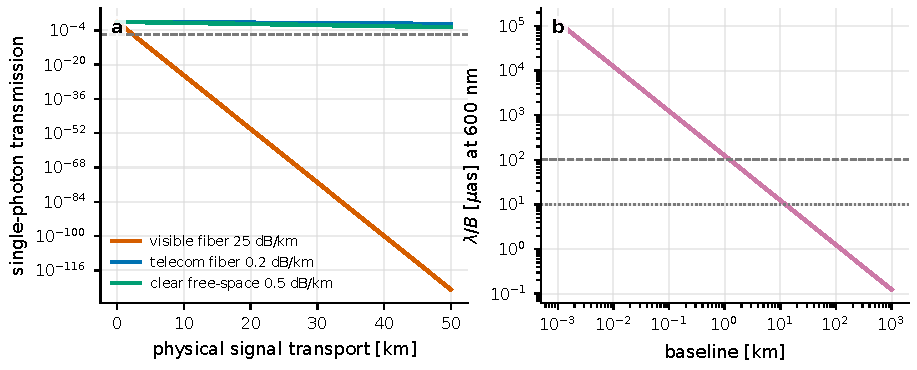
\includegraphics[width=0.94\linewidth]{figures/generated/chapter_17/ch17_architecture_loss.pdf}
\caption{长基线的吸引力和困难来自同一个量纲。左图把直接传输单光子星光的几种链路损耗画成透过率；可见光光纤在公里尺度已经严重衰减，telecom fiber 也会在百公里尺度变得昂贵。右图给出 \(\lambda/B\) 的角分辨率标度；600 nm 光在 1 km 基线达到百微角秒量级，100 km 基线进入微角秒量级。}
\label{fig:ch17-architecture-loss}
\end{figure}

角分辨率的基本标度是
\begin{equation}
  \theta_{\rm res}
  \sim
  \frac{\lambda}{B}
  =
  124\,\mu{\rm as}
  \left(\frac{\lambda}{600\,{\rm nm}}\right)
  \left(\frac{1\,{\rm km}}{B}\right).
  \label{eq:ch17-resolution-scale}
\end{equation}
\begin{formulaexplain}[公式 (17.4) 解读]
\(\theta_{\rm res}\) 是干涉角分辨率标度，\(B\) 是基线长度。基线越长，分辨率越高；量子网络方案追求的是在不传输未知星光的情况下把 \(B\) 推到 km 甚至更长。
\end{formulaexplain}
\(B=10\,{\rm km}\) 时是 \(12\,\mu{\rm as}\)，\(B=100\,{\rm km}\) 时是 \(1.2\,\mu{\rm as}\)。量子网络望远镜的吸引力就在这个尺度上：它不一定提高单孔径灵敏度，却可能把光学/近红外干涉从几百米推向 km、十 km 或更远的基线。HBT 强度干涉已经绕开了光学相位传输，但它主要给 \(|V|^2\)，灵敏度和相位恢复路线不同；量子网络路线的目标是保留一阶相干的相位信息，同时不把未知星光长距离搬运 \citep{1956Natur.178.1046H,2014A&G....55c3.28K,2016OptL...41.1094K,2023OExpr..3144246C,2024SPIE13095E..1NR}。

\section{预共享纠缠怎样替代传星光}

Gottesman-Jennewein-Croke 方案用一个已知的路径纠缠“实验室光子”
\begin{equation}
  |\Phi_\delta\rangle
  =
  \frac{|1\rangle_L|0\rangle_R
  +
  e^{i\delta}
  |0\rangle_L|1\rangle_R}{\sqrt2}
  \label{eq:ch17-lab-entangled-photon}
\end{equation}
\begin{formulaexplain}[公式 (17.5) 解读]
\(|\Phi_\delta\rangle\) 是预共享实验室路径纠缠光子，\(\delta\) 是可控相位。它替代了长距离搬运未知星光的任务：纠缠资源可以提前制备、验证，失败则丢弃重来。
\end{formulaexplain}
与未知星光光子做本地干涉。纠缠态可以提前通过量子网络分发；若分发失败，就重新来一次，不损失星光。星光到达后，两端各自把星光模式和实验室模式送入本地 beamsplitter，并只保留左右两边各探测到一个光子的事件。相关和反相关点击概率含有
\begin{equation}
  P_{\pm}(\delta)
  =
  \frac{1}{2}
  \left[
  1
  \pm
  {\rm Re}
  \left(
  V e^{-i\delta}
  \right)
  \right].
  \label{eq:ch17-gjc-probability}
\end{equation}
\begin{formulaexplain}[公式 (17.6) 解读]
\(P_\pm(\delta)\) 是两类符合点击概率，\(V\) 是星光复可见度，\(\delta\) 是实验室纠缠相位。改变 \(\delta\) 就像扫描参考相位，可以从点击率振荡中读出 \(V\) 的实部和虚部。
\end{formulaexplain}
扫描或改变 \(\delta\) 就可估计 \(V\) 的实部和虚部。这里的本地 beamsplitter 和符合探测相当于一次 Bell 态投影：星光模式和实验室纠缠模式的哪一路信息被擦除，只剩两条路径的相位关系。Bell 态测量就是把两个光子投影到一组最大纠缠的两模基上。线性光学只能无歧义地区分其中一部分点击组合，所以只有约一半有效星光事件进入估计；若能做完整 Bell 态测量或使用更复杂的量子处理，这个 \(50\%\) 损失可在原则上避免 \citep{1982Natur.299..802W,1993PhRvL..70.1895B,2012PhRvL.109g0503G}。

资源率是这条路线的第一道限制。若观测带宽是 \(\Delta\nu\)，相干时间约 \(1/\Delta\nu\)。直接 GJC 路线需要在每个可能有星光的相干时间窗准备匹配的纠缠光子；\(\Delta\nu=10\,{\rm GHz}\) 意味着每秒 \(10^{10}\) 个时间窗。Rajagopal 等给出的天文路线图指出，当前高质量 entangled-photon source 的典型速率距离这个数很远；GJC 更适合作为短基线 on-sky proof of principle，短期内还难以替代现有光学干涉阵列 \citep{2024SPIE13095E..1NR,2012PhRvL.109g0503G}。

Khabiboulline-Borregaard-De Greve-Lukin 方案利用弱光源的事实：每个长测量窗口内平均只有 \(\epsilon\ll1\) 个相关星光光子。把窗口分成 \(M\sim1/\epsilon\) 个 time bins 后，只有一个 time bin 可能含有光子。若用 unary code，需要 \(M\) 个 Bell pairs；若用 binary code，存下到达时间只需
\begin{equation}
  n_{\rm mem}
  =
  \left\lceil
  \log_2(M+1)
  \right\rceil
  \simeq
  \left\lceil
  \log_2(1/\epsilon)
  \right\rceil
  \label{eq:ch17-binary-timebin}
\end{equation}
\begin{formulaexplain}[公式 (17.7) 解读]
\(n_{\rm mem}\) 是需要的存储 qubit 数，\(M\) 是 time bins 数，\(\epsilon\) 是每个 bin 的平均星光光子数。弱光的稀疏性把资源从 \(M\) 个纠缠对降到 \(\log_2M\) 个存储位。
\end{formulaexplain}
个 memory qubits，每个 qubit pair 用一个 Bell pair 做非局域 parity check。若 \(M=10^6\)，约 20 个 qubits 就能编码到达时间，而 unary code 需要一百万个纠缠对。论文中的代表性量级是：对 \(\Delta f=1\,{\rm MHz}\)、1 s 测量窗口，\(N=10^6\) 个 time bins 对应 \(\log_2N\simeq20\)；在一个天文例子中，10 等星、\(10\,{\rm m^2}\) 收集面积和 \(10\,{\rm GHz}\) 检测带宽可导出约 \(20-30\) 个 qubits 与 \(\sim200\,{\rm kHz}\) 纠缠供应率的资源目标。Stas 等的补充分析也用 \(20\) 个 SiV 节点、1 kHz 零距离 entanglement rate 和 1 s 窗口展示了这种对数缩放的路径 \citep{2019PhRvL.123g0504K,2022PhRvA.106c2424C,2026Natur.651..326S,2024SPIE13095E..1NR}。

\begin{figure}[tbp]
\centering
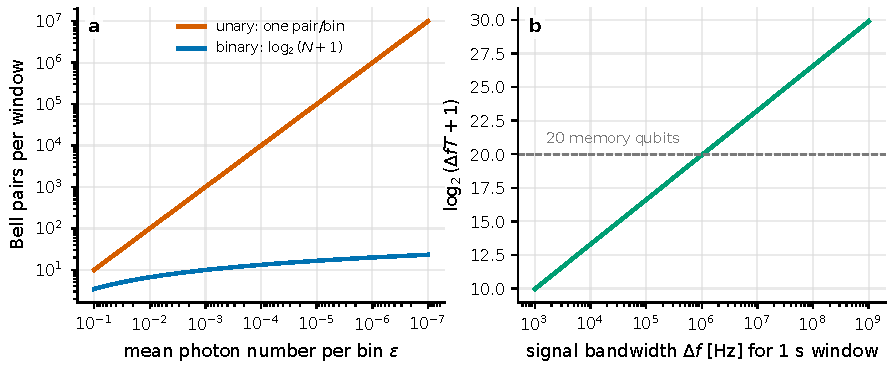
\includegraphics[width=0.94\linewidth]{figures/generated/chapter_17/ch17_timebin_scaling.pdf}
\caption{弱星光使 time-bin 编码有意义。左图比较 unary code 和 binary code 对 Bell pairs 的需求：当每个 bin 的平均光子数 \(\epsilon\) 很小，\(M\sim1/\epsilon\) 个 bin 可被 \(\log_2(M+1)\) 个 memory qubits 标记。右图显示 1 s 测量窗口中，1 MHz 带宽对应约 \(10^6\) 个 bin，也就是约 20 个 qubits。}
\label{fig:ch17-timebin}
\end{figure}

量子中继是这些方案的底层通信技术。直接传未知量子态受损耗和不可克隆定理限制；中继把总距离分段，先在短段内建立纠缠，再通过 entanglement swapping 连接长距离。理想中继可把指数损耗变成更温和的资源缩放，但真实系统还要面对 Bell-state measurement 成功率、memory lifetime、dark counts、gate fidelity 和 frequency conversion。DLCZ 原子系综协议、量子互联网路线和量子存储综述都把存储放在资源预算中心，因为它负责把概率成功事件同步起来 \citep{1998PhRvL..81.5932B,2001Natur.414..413D,2011RvMP...83...33S,2008Natur.453.1023K,2012IEEEN..26d..59V,2006quant.ph..7182U}。

\section{资源率、存储时间和保真度怎样闭合}

任何量子网络望远镜方案最后都要回到同一张账本。角分辨率由 \(B\) 给出，但能不能观测由资源率、存储时间、保真度和星光事件率共同决定；少一个环节，长基线的相位杠杆就无法兑现。第一个资源约束是纠缠供应率。若被接受的星光事件率是 \(R_\star\)，每个事件平均消耗 \(n_{\rm pair}\) 个 Bell pairs，则
\begin{equation}
  R_{\rm ent}
  \gtrsim
  \frac{n_{\rm pair}R_\star}{p_{\rm ready}},
  \label{eq:ch17-entanglement-rate}
\end{equation}
\begin{formulaexplain}[公式 (17.8) 解读]
\(R_{\rm ent}\) 是所需纠缠供应率，\(R_\star\) 是有效星光事件率，\(n_{\rm pair}\) 是每个事件消耗的 Bell pairs 数，\(p_{\rm ready}\) 是资源已就绪概率。它把天文事件率直接转成量子网络吞吐量要求。
\end{formulaexplain}
\(p_{\rm ready}\) 是星光到达时可用 Bell pairs 已经准备好的概率。\(R_\star\) 指进入目标空间模式、频率通道、偏振通道、时间窗并通过质量筛选后的事件率，不等同于望远镜总 photon rate。对宽带亮源，\(R_\star\) 可非常高，GJC 型方案会被资源率压垮；对窄带弱源，\(R_\star\) 小，memory-assisted scheme 才有机会用较低 \(R_{\rm ent}\) 换取长基线。

第二个资源约束是存储时间。最低限度，量子态或测量记录要等到经典通信和非局域校验完成：
\begin{equation}
  T_{\rm mem}
  \gtrsim
  \max\!\left[
    \frac{B}{c},
    T_{\rm ent},
    T_{\rm proc},
    T_{\rm win}
  \right].
  \label{eq:ch17-memory-time}
\end{equation}
\begin{formulaexplain}[公式 (17.9) 解读]
\(T_{\rm mem}\) 是量子存储必须保持相干的时间，右边取基线光行时、纠缠生成时间、处理时间和观测窗口的最大值。真正限制存储的常常不是 \(B/c\)，而是同步和 time-bin 窗口。
\end{formulaexplain}
\(B/c=3.3\,\mu{\rm s}\,(B/{\rm km})\)。\(100\,{\rm km}\) 基线只需 \(0.33\,{\rm ms}\) 的光行时，但 Khabiboulline 型二进制 time-bin 方案还可能需要 \(T_{\rm win}\sim1\,{\rm s}\) 的测量窗口来覆盖窄带弱光；这比光行时要求严得多。量子存储文献通常用 fidelity、efficiency、storage time、bandwidth、multimode capacity 和 wavelength 六个指标描述硬件。单光子存储的 conditional fidelity 是读出的波包与写入波包的重合度，efficiency 是成功读出光子的概率；对未知光态 teleportation 或非局域干涉，二者的乘积、相位噪声和模式匹配都进入最终 visibility \citep{2009NaPho...3..706L,2010EPJD...58....1S,2016JMOp...63.2005H}。

\begin{figure}[tbp]
\centering
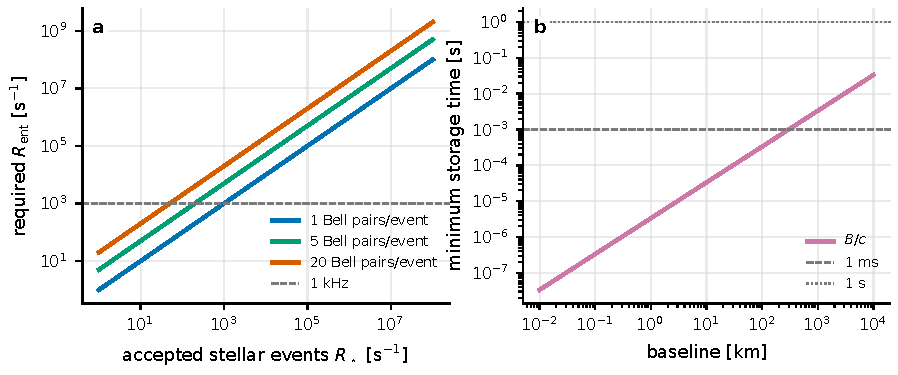
\includegraphics[width=0.94\linewidth]{figures/generated/chapter_17/ch17_entanglement_resources.pdf}
\caption{纠缠率和存储时间给出第一层资源闭合条件。左图把被接受的星光事件率 \(R_\star\) 转成 Bell pair rate；每个事件消耗的纠缠对越多，需求线越高。右图把基线转为 \(B/c\)；对 km 级基线，光行时是微秒到毫秒，但窄带存储方案常由测量窗口和纠缠生成时间决定。}
\label{fig:ch17-entanglement-resources}
\end{figure}

资源预算里常把链路中几个主要损失因子乘在一起，得到一个有效保真度标度：
\begin{equation}
  F_{\rm eff}
  \simeq
  F_{\rm Bell}
  \eta_{\rm write}
  \eta_{\rm read}
  \eta_{\rm conv}
  \exp(-T/T_2)
  (1-p_{\rm dark})
  M_{\rm mode}.
  \label{eq:ch17-effective-fidelity}
\end{equation}
\begin{formulaexplain}[公式 (17.10) 解读]
\(F_{\rm eff}\) 是粗略有效资源质量，包含 Bell pair 保真度、写入/读出效率、频率转换、存储退相干、暗触发和模式匹配。任何一项偏低都会乘法式降低最终可见度。
\end{formulaexplain}
\(F_{\rm Bell}\) 是预共享 Bell pair fidelity；\(\eta_{\rm write}\)、\(\eta_{\rm read}\) 是写入和读出效率；\(\eta_{\rm conv}\) 是频率转换效率；\(T_2\) 是相干时间；\(p_{\rm dark}\) 是等效暗触发概率；\(M_{\rm mode}\le1\) 表示频率、时间、偏振和空间模式匹配。这个式子不是完整量子信道模型，但它能快速暴露瓶颈。例如 \(T/T_2=1\) 单独就给 \(e^{-1}\simeq0.37\) 的相干因子；若 \(F_{\rm Bell}=0.8\)、读写各 \(0.7\)、转换 \(0.8\)，还没算暗计数和模式失配，乘积已降到 \(\sim0.3\)。

\begin{figure}[tbp]
\centering
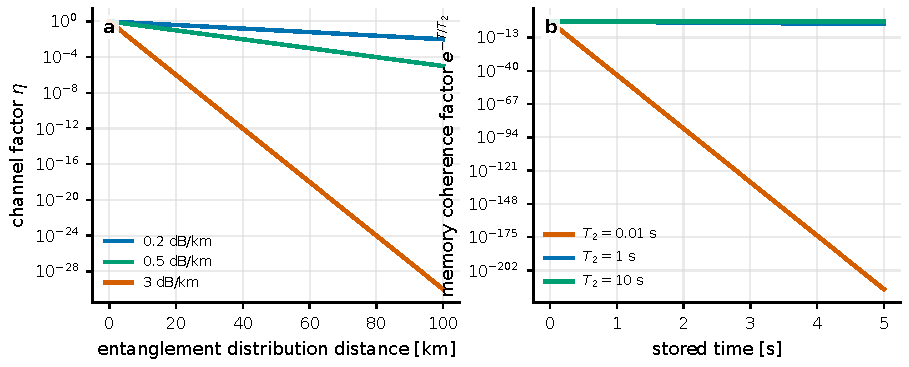
\includegraphics[width=0.94\linewidth]{figures/generated/chapter_17/ch17_fidelity_distance.pdf}
\caption{有效资源质量由链路和存储共同决定。左图显示不同 dB/km 损耗下的通道因子；右图显示存储时间与 \(T_2\) 的关系。一个长基线方案即使角分辨率诱人，也要让 Bell pair fidelity、读写效率、频率转换和存储相干同时闭合。}
\label{fig:ch17-fidelity-distance}
\end{figure}

频率转换是天文版本的额外难题。许多量子存储材料的强耦合频率不在目标天文波段；长距离光纤又偏好 telecom band。量子频率转换要在保持单光子相干、偏振或 time-bin 编码的同时降低噪声。若目标是和星光做干涉，转换后的谱宽、中心频率、时间波包和偏振都要和星光模式匹配；一个 \(1\%\) 的模式失配不会只损失 \(1\%\) 光子数，它会直接降低干涉 visibility \citep{1990OptL...15.1476K,2010EPJD...58....1S,2016JMOp...63.2005H,2024SPIE13095E..1NR}。

\section{连续变量和辅助单光子路线各解决什么}

前面的方案把路径自由度看成离散 qubit，并把时间窗或到达时间写进存储。还有两类互补想法：连续变量路线试图直接传送光场正交分量，辅助单光子路线则把可损失的实验室光子拿来承担长距离链路风险。它们解决的瓶颈不同，也带来不同资源成本。

这里的连续变量指光场的两个正交分量，而不是“左/右路径”这样的离散 qubit。连续变量 teleportation 用预共享的两模压缩真空态和本地测量，把一个模式的正交分量信息转移到远端模式。若资源态是
\begin{equation}
  |\psi_{\rm TMSV}\rangle
  =
  \sqrt{1-\lambda^2}
  \sum_{n=0}^{\infty}
  \lambda^n |n\rangle_A|n\rangle_B,
  \qquad
  \bar N = 2\sinh^2 r,
  \label{eq:ch17-tmsv}
\end{equation}
\begin{formulaexplain}[公式 (17.11) 解读]
\(|\psi_{\rm TMSV}\rangle\) 是两模压缩真空资源态，\(\lambda\) 或 \(r\) 控制压缩强度，\(\bar N\) 是总平均光子数。压缩越强，连续变量 teleportation 的附加噪声越小，但资源成本越高。
\end{formulaexplain}
\(r\) 是 squeezing parameter，\(\bar N\) 是两模总平均光子数。理想 \(r\to\infty\) 才能无噪声 teleport 任意连续变量态；有限 \(r\) 会加入等效高斯噪声，常按 \(e^{-2r}\) 标度下降。Gottesman 等已经指出，CV teleportation 可避免单 qubit Bell measurement 的 \(50\%\) 限制，但连续变量中继和远距离高保真压缩资源更难。最新 optimality 分析还提醒，比较不同资源态时要考虑 photon-number superselection rule、locality 和有限 entanglement budget；压缩度只是资源账本中的一项 \citep{1998PhRvL..80..869B,2012PhRvL.109g0503G,2025PhRvR...7d3278Z}。

另一条近中期路线不依赖长寿命量子存储，而是用本地或地面产生的单光子辅助星光干涉。Marchese-Kok 方案把星光光子尽早在接收端测量，让辅助单光子跨基线传输；损耗主要作用在“可重来的”地面光子上。对小角度位置估计，相位和角度满足
\begin{equation}
  \phi
  =
  \frac{2\pi B\theta}{\lambda},
  \qquad
  \sigma_\theta
  \ge
  \frac{\lambda}{2\pi B}
  \frac{1}{\sqrt{N_{\rm ev}\mathcal F_\phi}},
  \label{eq:ch17-angle-fisher}
\end{equation}
\begin{formulaexplain}[公式 (17.12) 解读]
\(\phi\) 是角位置 \(\theta\) 对应的干涉相位，\(\sigma_\theta\) 是角度误差下限，\(N_{\rm ev}\) 是有效事件数，\(\mathcal F_\phi\) 是单事件相位 Fisher 信息。基线越长、事件越多、单事件信息越高，定位越精。
\end{formulaexplain}
\(N_{\rm ev}\) 是有效事件数，\(\mathcal F_\phi\) 是单事件相位 Fisher 信息。Marchese-Kok 在 \(\lambda=628\,{\rm nm}\)、光纤 attenuation length \(L_0=10\,{\rm km}\) 的模型中得到十几 \(\mu{\rm as}\) 量级的定位标度；Modak-Kok 进一步指出，星光模式占据数 \(\epsilon\ll1\) 和辅助光子与星光的不可区分度会显著改变收益。若 \(\epsilon\) 从 1 降到 \(0.01\)，增加辅助光子数的优势会很快变弱；若模式不可区分度只有 \(96\%\)，三光子方案还可能有收益，但更高光子数不一定继续改善 \citep{2023PhRvL.130p0801M,2025PhRvA.111d3701M}。

Padilla、Sajjad、Saif 和 Guha 的分布式纠缠成像工作把这个问题推进到更一般的多模成像极限：先在每个接收站做本地空间模式排序，再用预共享 Bell pairs 模拟非局域 beamsplitter 或更一般的干涉网络。长基线只是资源的一部分；单孔径内的模式信息、源结构先验、阵列几何和测量基选择都会改变 Fisher 信息。对双星角分离，若只追求 Rayleigh 标度下的 \(\lambda/B\)，可能错过本地模式排序带来的小分离优势；若只追求本地 superresolution，又得不到长基线提供的相位杠杆 \citep{2026PhRvA.113a2608P,2025PhRvR...7d3278Z}。

\section{实验原型怎样转成误差预算}

实验原型的价值不只是证明“能纠缠两个远端节点”，而是给资源账本里的每一项填上可测数字。Stas 等的 2026 年实验把“非局域相位测量”从线路图推到实验台。他们用两个 SiV diamond nanocavity 节点、电子自旋和 \({}^{29}{\rm Si}\) nuclear-spin memory，先生成远程 Bell pair，再让弱信号光在本地与节点相互作用，通过 photon erasure 和非局域 non-destructive heralding 过滤真空事件。实验中 electron Bell state 可达 \(F=0.83(3)\)，entanglement rate 为 \(13\,{\rm Hz}\) 时 \(F\ge0.5\)，为 \(1.9\,{\rm Hz}\) 时 \(F=0.79(3)\)。完整非局域相位测量中，heralding 后 visibility 从无 heralding 的 \(0.031(18)\) 提高到 \(0.090(26)\)；加入 \(1.55\,{\rm km}\) 光纤基线后，nuclear parity oscillation visibility 为 \(0.11(4)\)，Bell pair fidelity 仍高于可验证纠缠阈值，约 \(F=0.63(3)\) \citep{2026Natur.651..326S}。

这类实验的相位误差由有效试验次数、herald 成功率和测得的相位振荡 visibility 共同决定。用 Fisher 信息表示时，
\begin{equation}
  \mathcal I_\phi
  \simeq
  N_{\rm tr}\,
  p_{\rm succ}\,
  V_{\rm meas}^2,
  \qquad
  {\rm Var}(\hat\phi)\ge \mathcal I_\phi^{-1}.
  \label{eq:ch17-fisher-visibility}
\end{equation}
\begin{formulaexplain}[公式 (17.13) 解读]
\(\mathcal I_\phi\) 是总相位 Fisher 信息，\(N_{\rm tr}\) 是试验次数，\(p_{\rm succ}\) 是 herald 成功率，\(V_{\rm meas}\) 是测得可见度。可见度以平方进入信息量，所以少量相干损失会明显放大相位误差。
\end{formulaexplain}
\(N_{\rm tr}\) 是 protocol trials 数，\(p_{\rm succ}\) 是成功 herald 的概率，\(V_{\rm meas}\) 是相位振荡 visibility。Stas 等给出的实现中
\begin{equation}
  p_{\rm succ}
  =
  \eta_{\rm erasure}\eta_{\rm herald}
  P(n_{\rm photon}\ge1),
  \label{eq:ch17-psucc}
\end{equation}
\begin{formulaexplain}[公式 (17.14) 解读]
\(p_{\rm succ}\) 是一次试验被接受的概率，包含 photon erasure、herald 探测和至少一个光子到达的概率。提高它不能只靠加大光强；多光子污染会降低 visibility，反而减少总 Fisher 信息。
\end{formulaexplain}
多光子事件、mis-heralding 和 Bell state infidelity 会降低 \(V_{\rm meas}\)。这解释了为什么“herald 成功率高”不一定好：若通过提高平均光子数获得更多 herald，却引入多光子污染，visibility 可能下降，\(\mathcal I_\phi\) 不升反降。相位误差再用式 \eqref{eq:ch17-angle-fisher} 转成角度误差；\(B\) 越长，相同 \(\sigma_\phi\) 对应越小 \(\sigma_\theta\)，但长基线也会增加 entanglement distribution overhead、相位锁定难度和延迟。

\begin{figure}[tbp]
\centering
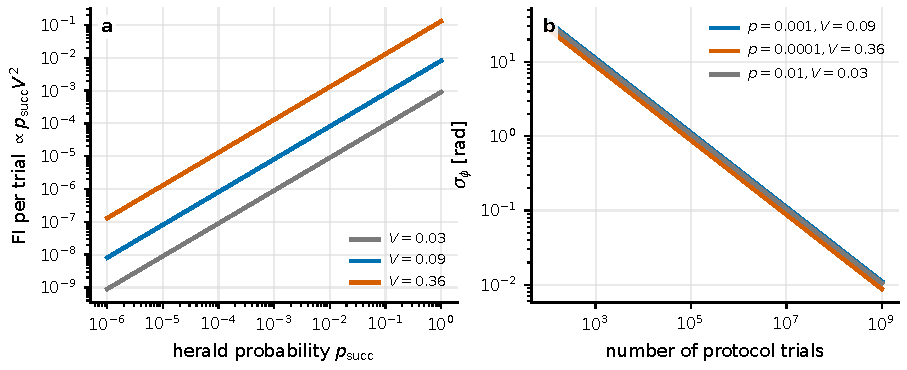
\includegraphics[width=0.94\linewidth]{figures/generated/chapter_17/ch17_fisher_visibility.pdf}
\caption{非局域相位测量的统计收益同时依赖成功概率和可见度。左图画出单 trial Fisher 信息的标度 \(p_{\rm succ}V^2\)；visibility 降低三倍，信息降低九倍。右图把 trial 数转成相位误差，显示高重复率、低 mis-herald 和高 Bell fidelity 要同时成立。}
\label{fig:ch17-fisher-visibility}
\end{figure}

Crawford 等的两光子精密天体测量实验提供了另一种近期台阶：用两个准热光源和时间标记探测器，在 benchtop analogue 中看到 photon-pair coincidence 随相位变化的相关行为。这个实验不等同于完整量子网络望远镜，但它很适合作为 on-sky 前的验证：时间标记、polarization matching、coherence time、HBT peak fitting、phase stability 和数据筛选都和真实天文弱光相关 \citep{2023OExpr..3144246C}。

把所有资源放在同一张图里，近期实验大致处在 \(R_{\rm ent}\sim1-10\,{\rm Hz}\)、短基线、低有效 visibility 区域；天文可用的 memory-assisted narrowband 方案可能需要 \(R_{\rm ent}\sim{\rm kHz}\) 到 \(100\,{\rm kHz}\)、\(T_{\rm mem}\sim{\rm ms}\) 到 s、几十个 memory qubits 和高模式匹配；宽带成像则更难。资源约束要一起闭合：\(R_{\rm ent}\) 不够会浪费星光事件，\(T_{\rm mem}\) 不够会让 parity check 赶不上，\(F_{\rm eff}\) 不够会洗掉 visibility，\(R_\star\) 估错会让整套方案在第一晚观测前就失去可行性。

\begin{figure}[tbp]
\centering
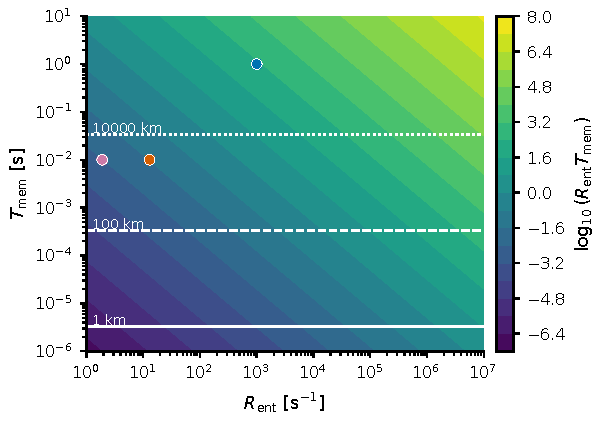
\includegraphics[width=0.94\linewidth]{figures/generated/chapter_17/ch17_network_parameter_space.pdf}
\caption{量子网络望远镜的资源空间由纠缠率和存储时间共同决定。白线标出 1 km、100 km 和 \(10^4\) km 基线的 \(B/c\) 时间；散点给出当前实验 Hz 级纠缠率和远期 kHz-s 级目标的量级。颜色只是资源乘积标度，完整可行性还要乘上 fidelity、模式匹配和天文光子率。}
\label{fig:ch17-network-space}
\end{figure}

\section{量子网络和强度干涉怎样互补}

量子网络望远镜不应被写成强度干涉的替代品，而应被写成长期互补路线。强度干涉已经能用本地时间标记和离线相关绕开光学相位传输，代价是主要得到 \(|V|^2\)；量子网络路线想保留一阶相干的相位信息，代价是要支付纠缠、存储、转换和 heralding 的资源账本。短期内仍要和 ELT、VLTI、CHARA、CTAO 或强度干涉阵列并行发展。近期目标是强度干涉和两光子相关：硬件接近已有大面积光收集器、SNSPD/SPAD 时间标记、窄带滤波和离线相关，科学目标集中在亮星角直径、双星和发射线区域。下一步加入本地模式排序、two-photon astrometry 和 GJC 型短基线 on-sky 演示，目标是证明星光模式可和实验室纠缠资源稳定干涉。memory-assisted 非局域一阶相干测量需要量子存储、频率转换、纠缠分发、Bell fidelity 和天文仪器同步共同成熟，应放在更远期的技术目标中 \citep{1956Natur.178.1046H,2023OExpr..3144246C,2024SPIE13095E..1NR,2026Natur.651..326S}。

\Needspace{11\baselineskip}
观测规划可以从一个简单闭合条件开始：
\begin{equation}
  N_{\rm useful}
  =
  R_\star T_{\rm obs}
  p_{\rm ready}
  p_{\rm succ}
  V_{\rm meas}^2
  \gtrsim
  N_{\rm req}(\sigma_\theta,{\bf B},\lambda).
  \label{eq:ch17-useful-events}
\end{equation}
\begin{formulaexplain}[公式 (17.15) 解读]
\(N_{\rm useful}\) 是真正有相位信息的有效事件数，等于星光事件率、观测时间、资源就绪概率、成功率和可见度平方的乘积。它必须超过目标精度所需的 \(N_{\rm req}\)，方案才有观测意义。
\end{formulaexplain}
\(T_{\rm obs}\) 是总观测时间；\(N_{\rm req}\) 由目标角精度、阵列几何和模型参数维数决定。这个式子把天文学和量子工程放在同一张账本上：亮源、窄带、已知到达时间或周期信号会降低资源压力；暗弱宽带连续源会把所有困难放大。同样的账本也适用于更一般的观测设计，只是可观测量从非局域相位换成 \(|V|^2\)、\(g^{(2)}\)、偏振角或时间延迟。

量子网络望远镜目前最有价值的是这张可行性账本，而不是某个已经成熟的仪器方案。下一部分回到观测设计：科学参数需要落到事件率、通道、基线、背景和协方差上，然后才谈得上选择强度干涉、偏振事件表、瞬变触发或未来非局域相位测量。


\part[观测设计、案例、教学和路线图]{观测设计、案例、教学和路线图}
\chapter{观测设计、误差预算和可行性计算}
\label{chap:18}

\begin{chapteropening}
观测设计从待测物理参数开始，再倒推望远镜和仪器设置。要测恒星角直径，就要知道 \(|V|^2(B,\lambda)\) 在哪些基线最敏感；要测强度相关，就要知道零延迟相关峰有多高、探测器会把它稀释到什么程度；要测偏振旋转或时间延迟，就要知道事件表里时间、频率和偏振标签的精度。强度干涉从 Hanbury Brown--Twiss 的 Sirius 实验、Narrabri 的 32 颗恒星角直径测量，到 VERITAS、MAGIC 和 photon-counting Vega 实验，使用的都是同一张可行性账本：光子率给出统计上限，相关 contrast 给出目标信号，基线、带宽、时间分辨率和校准误差决定这个信号能否留下来 \citep{1956Natur.178.1046H,1957RSPSA.242..300B,1958RSPSA.248..222B,1974MNRAS.167..121H,2006ApJ...649..399L,2020NatAs...4.1164A,2020MNRAS.491.1540A,2021MNRAS.506.1585Z}。
\end{chapteropening}

\section{从科学参数到事件表}

每个科学目标都对应一组待估计的物理参数 \(\boldsymbol\theta_{\rm phys}\)：恒星角直径、双星角分离、旋转星的扁率和位置角、谱线发射区半径、偏振角旋转、时延，或二阶相关峰的 contrast。仪器直接给出的是第 \ref{chap:01} 章式 \eqref{eq:event-row} 和第 \ref{chap:06} 章式 \eqref{eq:ch06-raw-event} 所描述的事件表，物理参数要从这些事件字段中估计。

观测设计从这些字段是否支撑目标参数开始：时间戳能否做 ns 相关，位置标签能否给出所需基线，波长和偏振标签是否保留，质量标记能否追踪天空背景、死时间、云量和时钟状态。若一开始只生成一张积分图像，后来想恢复 ns 时间相关或偏振相关，信息已经被平均掉；若保留事件表，后面可以投影成光变曲线、\(g^{(2)}(\tau)\)、\(|V|^2(B)\)、偏振角，或多波长 \(u,v\) 数据。

从参数到数据的关系可以写成
\begin{equation}
  \mathcal L(\boldsymbol\theta_{\rm phys})
  =
  P\!\left(d\,\middle|\,
  q_{\rm inst}(\boldsymbol\theta_{\rm phys}),
  {\bf c}_{\rm cal},
  {\bf b}_{\rm sky}
  \right).
  \label{eq:ch18-likelihood-chain}
\end{equation}
\begin{formulaexplain}[公式 (18.1) 解读]
\(\boldsymbol\theta_{\rm phys}\) 是要估计的物理参数，\(d\) 是事件表或其统计量。公式说明：物理参数先变成仪器可测量 \(q_{\rm inst}\)，再和校准项、背景项一起决定数据似然。
\end{formulaexplain}
\(\mathcal L\) 是似然；\(q_{\rm inst}\) 是仪器可测量，如 \(|V|^2\)、\(g^{(2)}-1\)、偏振 Stokes 量或到达时间残差；\({\bf c}_{\rm cal}\) 是校准参数，包括时间零点、滤光片通带、探测器效率和背景修正；\({\bf b}_{\rm sky}\) 是天光、月光、暗计数和宿主背景。实际 proposal 里，与其只写“我们会观测这颗星”，更有用的是写清这颗星的 \(m_B\)、\(\theta\)、可见窗口和模型先验会给出哪些 \(|V|^2\) 数据点，最终把 \(\theta\) 的误差压到多少。

角尺度先决定基线。空间频率、可见度和天空亮度的 Fourier 关系在第 \ref{chap:05} 章式 \eqref{eq:ch05-uv} 和 \eqref{eq:ch05-vcz} 中给出；观测设计直接用它的物理含义：振幅干涉测 \(V\) 的幅度和相位，强度干涉在热光近似下测 \(|V|^2\)。因此观测申请需要写清目标角尺度落在第几 lobe、需要哪些投影基线和位置角，以及相位缺失是否会导致模型退化 \citep{2003RPPh...66..789M,2009A&A...507.1719F,2012NewAR..56..143D,2014MNRAS.437..798M,2022MNRAS.512.1722K}。

粗略分辨率可用
\begin{equation}
  B
  \sim
  \frac{\lambda}{\theta}
  =
  86\,{\rm m}
  \left(\frac{\lambda}{416\,{\rm nm}}\right)
  \left(\frac{1\,{\rm mas}}{\theta}\right).
  \label{eq:ch18-baseline-scale}
\end{equation}
\begin{formulaexplain}[公式 (18.2) 解读]
\(B\) 是所需基线，\(\lambda\) 是观测波长，\(\theta\) 是目标角尺度。这个量级式把“要分辨多小”直接换成“需要多长基线”。
\end{formulaexplain}
\(\theta=2\,{\rm mas}\) 的热星在 416 nm 只需 \(\sim43\,{\rm m}\) 就开始被解析；\(\theta=0.5\,{\rm mas}\) 需要 \(\sim170\,{\rm m}\)；\(\theta=0.1\,{\rm mas}\) 进入 \(\sim860\,{\rm m}\) 级。Narrabri 的最大基线约 188 m，因此最擅长亮而热、角直径在几十分之一到几 mas 的恒星；CTA 型 km 阵列把空间频率推进到几十微角秒量级，但目标还要有足够光子率 \citep{1974MNRAS.167..121H,2006ApJ...649..399L,2010SPIE.7734E..1TJ,2013APh....43..331D}。

\section{光子率、带宽和相干稀释怎样决定可检性}

光子率从星等开始。AB 星等先换成谱流量密度：
\begin{equation}
  F_\nu=3631\,{\rm Jy}\,10^{-0.4m_{\rm AB}}.
  \label{eq:ch18-ab-flux}
\end{equation}
\begin{formulaexplain}[公式 (18.3) 解读]
\(m_{\rm AB}\) 是 AB 星等，\(F_\nu\) 是谱流量密度。星等每增加 5 等，\(F_\nu\) 下降 100 倍，因此光子率和相关信号也迅速变难。
\end{formulaexplain}
然后用第 \ref{chap:01} 章式 \eqref{eq:photon-rate} 把能量流量换成光子率。代入 550 nm、10 nm 通带和 \(\eta=0.25\)，一台 12 m 望远镜对 \(m_{\rm AB}=5\) 的源给出 \(R_\gamma\simeq2.8\times10^8\,{\rm s^{-1}}\)，对 \(m_{\rm AB}=8\) 给出 \(1.8\times10^7\,{\rm s^{-1}}\)。17 m MAGIC 级口径在同样假设下约为 \(5.7\times10^8\,{\rm s^{-1}}\) 和 \(3.6\times10^7\,{\rm s^{-1}}\)。这些数还不是可用相关事件率；它们会被空间模式、偏振、滤光片角入射、死时间、数据质量切片和背景修正继续削减 \citep{2006ApJ...649..399L,2020MNRAS.491.1540A,2021MNRAS.506.1585Z,2024MNRAS.529.4387A}。

\begin{figure}[tbp]
\centering
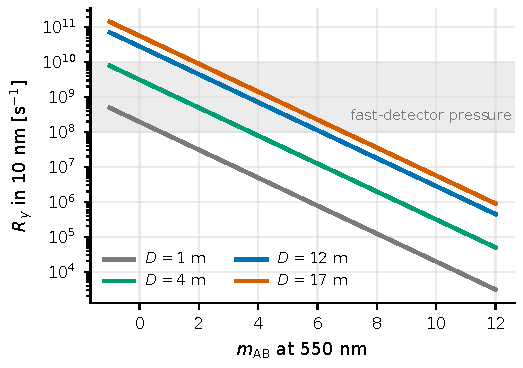
\includegraphics[width=0.86\linewidth]{figures/generated/chapter_18/ch18_photon_rate_magnitude.pdf}
\caption{AB 星等到窄带光子率的换算。曲线采用 550 nm、10 nm 通带和总效率 \(\eta=0.25\)。口径只线性改变收集面积，星等每增加 5 等会让光子率下降 100 倍；灰色区域标出 \(10^8\,{\rm s^{-1}}\) 以上的高速探测和数据吞吐压力。}
\label{fig:ch18-photon-rate}
\end{figure}

强度相关信号的高度由光学相干时间和电子响应共同决定。相干时间的带宽换算见第 \ref{chap:04} 章式 \eqref{eq:ch04-coherence-time}，热光峰的时间稀释见第 \ref{chap:04} 章式 \eqref{eq:ch04-contrast-dilution}。代入 VERITAS 常用的 416 nm、13 nm 通带，可得 \(\tau_c\simeq4.4\times10^{-14}\,{\rm s}\)；若探测器和电子链的等效时间宽度是 \(\Delta t=4\,{\rm ns}\)，未解析热光的零基线二阶相关峰自然落到几 \(10^{-6}\) 的量级。VERITAS 论文中测到的零基线归一化相关量 \(N_0\sim10^{-6}\) 处在同一量级；实际值还包含滤光片形状、探测器响应、偏振、背景和电子链修正 \citep{2020NatAs...4.1164A,2024ApJ...966...28A}。

\begin{figure}[tbp]
\centering
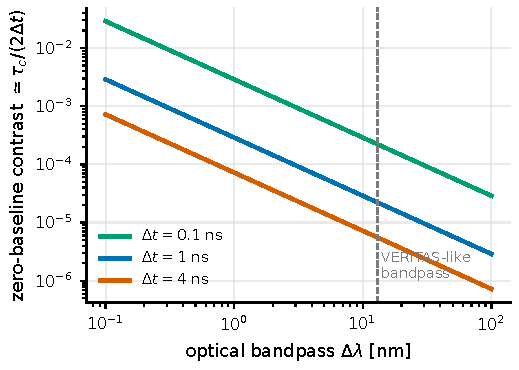
\includegraphics[width=0.86\linewidth]{figures/generated/chapter_18/ch18_coherence_dilution.pdf}
\caption{通带越宽，光学相干时间越短；电子时间分辨率越慢，零延迟相关峰越被稀释。416 nm、13 nm、4 ns 的组合给出几 \(10^{-6}\) 的 contrast，因此相关峰要靠长时间平均和严格校准才能从噪声中浮现。}
\label{fig:ch18-coherence-dilution}
\end{figure}

光学通带并不按单调方式改善 SNR。对理想热光强度干涉，若电子带宽远小于光学带宽，SNR 对光学通带宽度的一阶依赖会近似抵消：窄带减少光子数，但增加相干时间；宽带增加光子数，但降低每个时间 bin 的相关 contrast。真实仪器仍然关心滤光片，因为 PMT 或 SPAD 电流、天空背景、滤光片角入射和谱线科学目标都会改变可用信号。MAGIC 的低 \(f/D\simeq1\) 光束会让干涉滤光片在不同入射角下中心波长移动，实际通带比平行光测量更宽、更偏蓝；这会降低相关峰形状和 SNR，需要用光学模型和实验标定一起处理 \citep{2020MNRAS.491.1540A,2024MNRAS.529.4387A,2021MNRAS.506.1585Z}。

\section{强度相关的 SNR 怎样做第一轮估算}

双望远镜强度干涉的经典 SNR 标度已在式 \eqref{eq:ch05-snr} 中给出。设计阶段直接把目标星等、望远镜面积、总效率、电子带宽、积分时间和目标基线上的 \(|V|^2\) 代入该式即可。LeBohec 和 Holder 用 \(A=100\,{\rm m^2}\)、\(\alpha=0.3\)、\(\Delta f=1\,{\rm GHz}\)、\(T=5\,{\rm h}\)、\(|V|^2=0.5\) 得到 \(m_V\simeq6.7\) 的 \(5\sigma\) 量级估算；同样条件下 \(m_V=5\) 可达到二十以上的 SNR，而 \(m_V=9\) 只剩亚 sigma \citep{2006ApJ...649..399L,2008AIPC..984..205L,2012NewAR..56..143D}。

\begin{figure}[tbp]
\centering
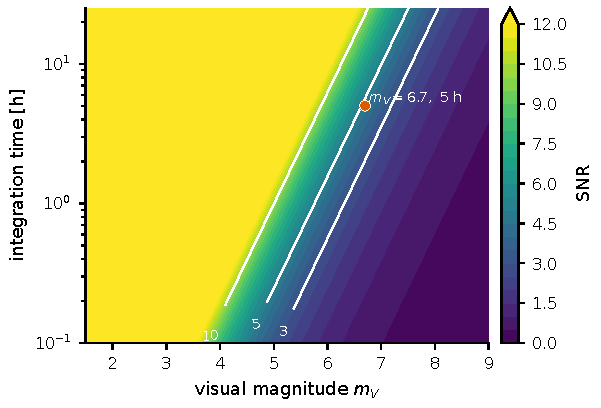
\includegraphics[width=0.90\linewidth]{figures/generated/chapter_18/ch18_snr_heatmap.pdf}
\caption{强度干涉 SNR 对星等和积分时间的依赖。图中采用 \(A=100\,{\rm m^2}\)、\(\alpha=0.3\)、\(\Delta f=1\,{\rm GHz}\)、\(|V|^2=0.5\)；橙点对应 LeBohec--Holder 估算中 \(m_V\simeq6.7\)、5 h 约 \(5\sigma\) 的位置。}
\label{fig:ch18-snr}
\end{figure}

式 \eqref{eq:ch05-snr} 只适合第一轮估算。真实数据里的 \(T\) 指通过质量切片后的有效 live time；\(\Delta f\) 指光学脉冲、PMT 或 SPAD 响应、线缆、放大器、digitizer 和软件相关共同形成的等效带宽；\(|V|^2\) 还会随目标高度和时角改变。VERITAS 的四台 12 m IACT 可同时给六条基线，采用 416 nm、\(\sim13\) nm 的滤光片和 4 ns 采样，每小时生成约 3.5 TB 原始数据；MAGIC 的两台 17 m 望远镜使用中央 PMT 和窄带滤光片，早期演示报告了比 Narrabri 约高一个数量级的灵敏度。Vega photon-counting 实验则展示了另一路线：用 SPAD 与软件相关在零基线得到 \(\langle g^{(2)}\rangle=1.0034\pm0.0008\)，在 \(\sim2\) km 投影基线上未检出相关，符合 Vega 约 3.3 mas 角直径已经被完全解析的预期 \citep{2020NatAs...4.1164A,2020MNRAS.491.1540A,2021MNRAS.506.1585Z,2024MNRAS.529.4387A}。

多基线同时增加数据量和几何信息。\(N\) 台望远镜给出 \(N(N-1)/2\) 条同时基线；4 台只有 6 条，60 台已有 1770 条。不同基线是在不同 \(u,v\) 点采样源结构，并非简单重复测量同一个数。若科学目标是一个均匀圆盘角直径，几条合适基线已经有用；若目标是快速旋转星的扁率、双星、盘风或非轴对称谱线发射区，就需要位置角覆盖。CTA 布局研究反复指出，长基线解析小尺度，但会丢掉整体形状；短基线测到总尺寸，却看不到高空间频率。覆盖 \(0.1-3\,{\rm mas}\) 的热星结构时，30--2000 m 的基线范围比单一最长基线更重要 \citep{2010SPIE.7734E..1CN,2010SPIE.7734E..1TJ,2012MNRAS.419..172N,2012MNRAS.424.1006N,2013MNRAS.430.3187R}。

\section{基线选择怎样变成参数灵敏度}

均匀圆盘是最常用的第一模型，其可见度和第一零点已在第 \ref{chap:05} 章式 \eqref{eq:ch05-uniform-disk} 和 \eqref{eq:ch05-first-null} 中给出。基线选择直接决定角直径信息量：若所有基线都在 \(|V|^2\simeq1\) 的平台上，不同 \(\theta\) 的曲线几乎重合；若只观测零点之后的极低可见度，相关峰又会接近噪声底。通常第一 lobe 下降区和第一零点附近给出最大的直径信息；limb darkening、快速自转和伴星会把曲线形状改掉，因此可行性计算要同时画目标模型的 \(|V|^2\) 和 \(\partial |V|^2/\partial\theta\) \citep{2003RPPh...66..789M,2020NatAs...4.1164A,2024ApJ...966...28A,2025ApJ...995..191A}。

\begin{figure}[tbp]
\centering
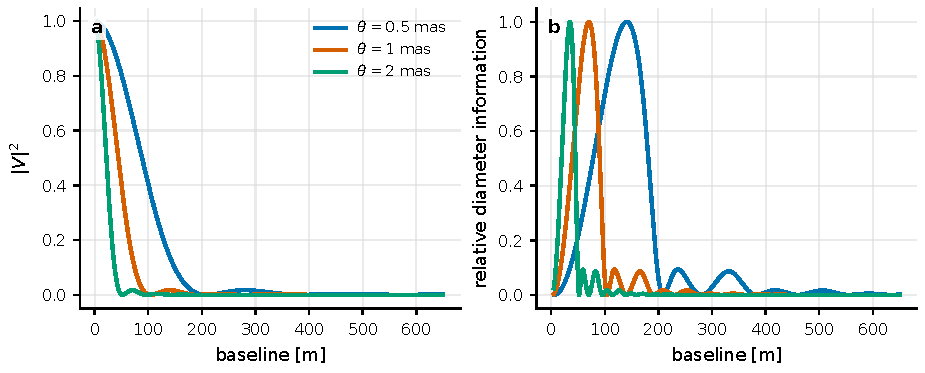
\includegraphics[width=0.94\linewidth]{figures/generated/chapter_18/ch18_visibility_fisher.pdf}
\caption{均匀圆盘的 \(|V|^2\) 曲线和直径灵敏度。416 nm 下，2 mas、1 mas 和 0.5 mas 目标的下降区分别落在几十米、百米和几百米基线；右图显示直径信息主要来自曲线斜率大的基线，短基线平台 \(|V|^2\simeq1\) 对直径不敏感。}
\label{fig:ch18-visibility-fisher}
\end{figure}

更一般的 Fisher 信息形式见第 \ref{chap:07} 章式 \eqref{eq:ch07-fisher} 和强度干涉专用的第 \ref{chap:08} 章式 \eqref{eq:ch08-sii-fisher}。在观测排程里，它的含义很直接：\(\mu_i\) 可以是 \(|V|^2\)、\(g^{(2)}\) 峰面积、偏振角或延迟；\(\sigma_i\) 应包含统计噪声和系统项。若某个基线的误差很小但导数几乎为零，它对目标参数几乎没有贡献；若导数大但 \(|V|^2\) 太低导致峰不可检出，也不能单独撑起结果。快速旋转星 \(\gamma\) Cas 的 VERITAS-SII 观测就是位置角覆盖的例子：不同投影基线采样不同方向的 \(|V|^2\)，从而约束扁率和长轴方向，单个等效圆盘直径不够描述这个目标 \citep{2025ApJ...995..191A,2024ApJ...966...28A}。

\begin{figure}[tbp]
\centering
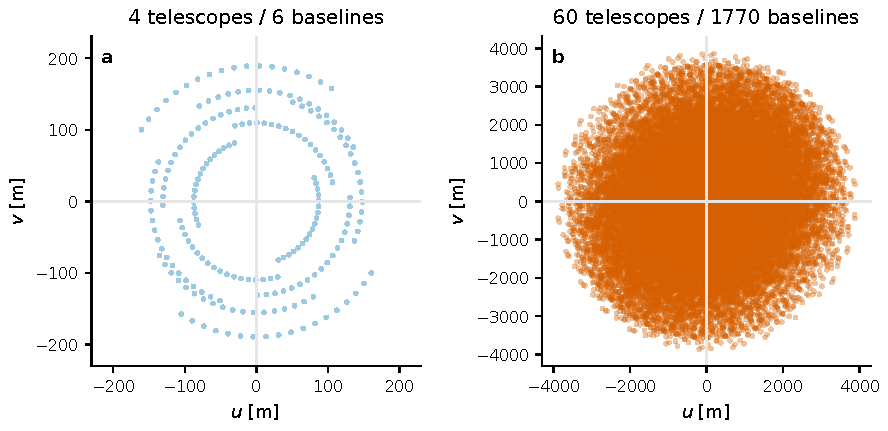
\includegraphics[width=0.94\linewidth]{figures/generated/chapter_18/ch18_uv_coverage.pdf}
\caption{阵列规模怎样改变 \(u,v\) 采样。左图是四台望远镜的示意覆盖，六条基线随时角旋转后仍较稀疏；右图是多望远镜 CTA 型阵列的示意覆盖，短基线、中等基线和长基线同时存在。密集覆盖不自动等于高 SNR，但它决定非轴对称目标能否被稳定拟合或重建。}
\label{fig:ch18-uv-coverage}
\end{figure}

波长也参与基线选择。同一物理基线在 416 nm 的空间频率比 800 nm 高约 1.9 倍；蓝端分辨率更高，但大气透过、镜面反射、探测量子效率和滤光片角入射更难。谱线观测还要考虑线通量而非宽带星等。对热星和 Be 星，H\(\alpha\)、He 或金属线可能来自比连续谱更大的发射区；窄带可以把几何结构和速度通道分开，但每个通道的事件率、滤光片泄漏和背景都要重新计算 \citep{2010SPIE.7734E..0AD,2012NewAR..56..143D,2021MNRAS.506.1585Z,2024MNRAS.529.4387A}。

\section{背景、校准和质量切片怎样进入系统误差}

背景不相关时，它主要稀释相关峰；两通道背景稀释因子的定义和假设已经在第 \ref{chap:06} 章式 \eqref{eq:ch06-background-dilution} 中给出。观测设计需要把这个修正落实到同一通道、同一增益状态和相近时间的背景测量上。VERITAS 的 \(\beta\) UMa 分析用目标附近 \(0.5^\circ\) 的 off runs 估计非星光电流，典型 off-source 强度约为 on-source 的 \(3\%\)，因此对半径拟合影响很小；明月、云、雾、城市光或 detector afterpulsing 会让这个近似变差，需要单独质量切片 \citep{2024ApJ...966...28A,2025ApJ...995..191A}。

\begin{figure}[tbp]
\centering
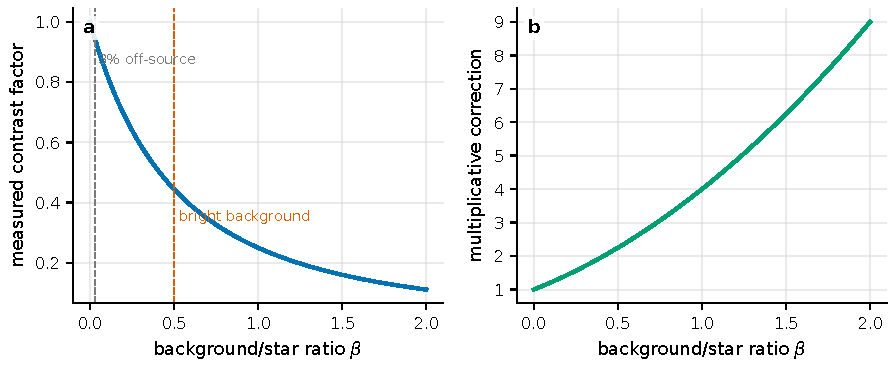
\includegraphics[width=0.94\linewidth]{figures/generated/chapter_18/ch18_background_dilution.pdf}
\caption{不相关背景对相关峰的稀释。若两端背景/星光比相同，观测 contrast 按 \((1+\beta)^{-2}\) 下降；\(\beta=0.03\) 只造成几个百分点修正，\(\beta=0.5\) 已把峰压到原来的约 44\%。右图给出反向修正因子，修正越大，对背景估计误差越敏感。}
\label{fig:ch18-background-dilution}
\end{figure}

时间校准是强度干涉和 photon counting 的共同硬件边界。相关峰宽度通常是几 ns；如果不同望远镜的相对延迟模型错了 1 ns，峰会被摊宽或移出拟合窗口。Vega photon-counting 实验中，零基线子孔径相对时间精度约 \(100\,{\rm ps}\)，两台望远镜之间还要处理光行时、仪器延迟、GPS 或 rubidium clock 漂移以及光纤色散，最终用 \(\sim400\,{\rm ps}\) time bin 做相关；他们指出多望远镜实现需要约 ns 级同步才能把观测时间保持在小时量级。VERITAS-SII 用 White Rabbit 10 MHz 时钟分发和 4 ns 采样，仍要在每个 run 中跟踪光程延迟随时角的变化，并处理 run-to-run 的峰位置变化 \citep{2021MNRAS.506.1585Z,2024ApJ...966...28A}。

校准星的选择要和科学目标同等认真。一个理想校准星应有已知角直径、稳定光度、接近目标的天空位置、相似颜色和足够高的光子率。若目标是 0.5 mas 热星，而校准星直径不确定到 \(5\%\)，最终直径误差很容易被校准项主导。现代强度干涉观测常把已知角直径热星作为 reference，先检查零基线归一化、滤光片响应和 \(|V|^2(B)\) 形状，再观测未知目标。MAGIC 2024 年的性能论文用多颗参考星验证系统，再给出新恒星角直径；VERITAS 的 \(\beta\) UMa 和 \(\gamma\) Cas 观测则展示了同一套系统从圆盘直径走向扁率和位置角测量 \citep{2024MNRAS.529.4387A,2024ApJ...966...28A,2025ApJ...995..191A}。

\section{误差预算怎样写进观测申请}

最终误差需要拆成统计项和系统项。对一个拟合参数 \(\theta\)，常用的误差预算为
\begin{equation}
  \sigma_\theta^2
  =
  \sigma_{\rm stat}^2
  +
  \sigma_{\rm bg}^2
  +
  \sigma_{\rm time}^2
  +
  \sigma_{\rm cal}^2
  +
  \sigma_{\rm model}^2 .
  \label{eq:ch18-error-budget}
\end{equation}
\begin{formulaexplain}[公式 (18.4) 解读]
\(\sigma_\theta\) 是目标参数的总误差，右边把统计、背景、时间、校准和模型误差分开。它提醒观测计划不能只报 SNR，还要说明误差平台来自哪里。
\end{formulaexplain}
\(\sigma_{\rm stat}\) 来自有限符合计数或相关峰拟合；\(\sigma_{\rm bg}\) 来自 off-source 背景插值和暗电流；\(\sigma_{\rm time}\) 来自时钟、几何延迟、采样和峰形；\(\sigma_{\rm cal}\) 来自校准星、throughput、滤光片和偏振；\(\sigma_{\rm model}\) 来自源模型，例如把快速旋转星当成圆盘、把谱线盘当成高斯、或忽略伴星。统计误差通常随 \(T^{-1/2}\) 下降，其他项常形成平台；当平台已经高于目标精度，继续加积分时间不会解决问题。

\begin{figure}[tbp]
\centering
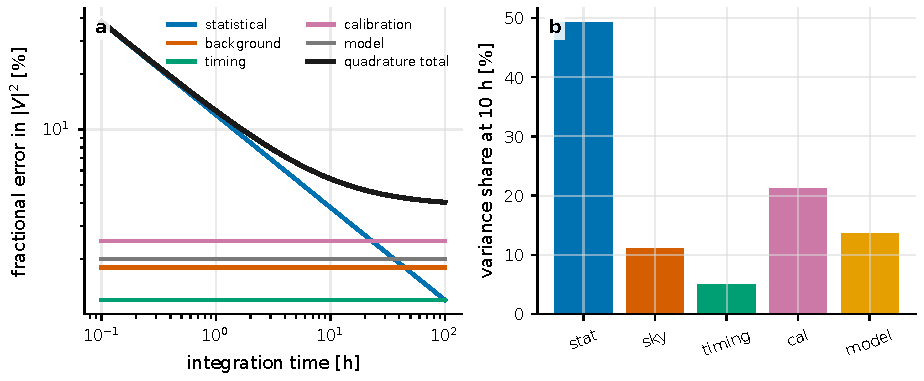
\includegraphics[width=0.94\linewidth]{figures/generated/chapter_18/ch18_error_budget.pdf}
\caption{误差预算中的统计项和系统项。左图显示统计误差随积分时间下降，但背景、时间、校准和模型项形成平台；右图把 10 h 时各项对总方差的贡献列出。观测申请应把每一项连接到可观测的校准数据，并给出总 SNR 之外的误差平台。}
\label{fig:ch18-error-budget}
\end{figure}

\begin{longtable}{p{0.18\linewidth}p{0.30\linewidth}p{0.42\linewidth}}
\toprule
量 & 常见范围 & 在计划中的用法 \\
\midrule
\(m_V,m_B\) & \(-1\) 到 \(9\) 等是当前 SII 的主战场 & 转成 \(n\) 或 \(R_\gamma\)，先判断目标是否过暗。 \\
\(A_{\rm eff}\) & \(1-250\,{\rm m^2}\) 每台望远镜 & 进入光子率和 SNR，镜面老化、遮挡和光纤耦合要算进效率。 \\
\(\Delta\lambda\) & \(0.1-30\,{\rm nm}\) & 决定相干时间、PMT 电流、天空背景和谱线选择。 \\
\(\Delta t\) & \(0.1-5\,{\rm ns}\) & 决定相关峰被稀释的程度和可用电子带宽。 \\
\(B_p\) & \(10-2000\,{\rm m}\) & 决定角尺度和 \(u,v\) 覆盖；短基线和长基线约束不同结构。 \\
\(\beta\) & \(0.01-1\) & 背景/星光比，决定 contrast 稀释和背景系统误差。 \\
\(\sigma_{\rm cal}\) & \(1-10\%\) 的可见度或直径量级 & 常成为长积分后的误差平台。 \\
\bottomrule
\end{longtable}

一份可执行的观测申请从目标参数写起，例如“测量 \(\gamma\) Cas 蓝光 photosphere 的长短轴比到 \(5\%\)”或“测量 1 mas A 型星的 limb-darkened 直径到 \(3\%\)”。目标描述随后给出星等、颜色、角直径估计、可见窗口，以及已有 CHARA/VLTI/Keck 或 Narrabri 数据。仪器部分要把望远镜数量、基线范围、滤光片中心波长和带宽、采样时间、同步方案、数据率和质量切片写清。

SNR 应按最有信息量的基线分别报告：统计精度来自式 \eqref{eq:ch05-snr}，背景修正来自式 \eqref{eq:ch06-background-dilution}，系统项则进入式 \eqref{eq:ch18-error-budget}。成功标准也要量化，例如至少三条基线在第一 lobe 下降区达到 \({\rm SNR}>5\)，校准星重复观测给出小于 \(3\%\) 的归一化漂移，off-source 背景修正小于总信号的 \(10\%\)。若长基线未检出，结果仍可给出角直径上限或排除过大的发射区；若校准平台过高，也能反推出仪器升级所需的时间同步、滤光片或背景控制指标。

这条估算链条同样适用于强度干涉之外的项目。振幅干涉、量子网络望远镜、CMB 偏振、FRB photon statistics 和实验室教学台架都需要同样的结构：事件率、模式数、响应函数、校准项、模型导数和误差预算。差别只在可观测量 \(\mu_i\) 的形式。科学案例排序也要沿用这个思路，把“科学价值”与“可观测性”分开评分，避免把漂亮目标和可执行目标混在一起 \citep{2010SPIE.7734E..0AD,2012MNRAS.419..172N,2012MNRAS.424.1006N,2013APh....43..331D,2014SPIE.9146E..0ZD,2017MNRAS.472.4126G,2022SPIE12183E..0DK,2024SPIE13095E..0IT,2026arXiv260212717K}。


\chapter{第一代量子天文学科学案例}
\label{chap:19}

\begin{chapteropening}
第一代科学案例要同时满足光子率、角尺度、基线覆盖、校准难度和失败后仍有用的科学产出。强度干涉已经从 Sirius 和 Narrabri 的亮星角直径，发展到 VERITAS、MAGIC、Vega photon-counting 和新近的快速自转星测量；这些结果把起点指向明亮、热、小角尺度、外部先验充足的目标。恒星角直径、快速自转、密近双星、Be/WR 谱线区、新星早期膨胀、Crab 光子统计和自然激光候选，构成第一批最现实的项目清单 \citep{1956Natur.178.1046H,1974MNRAS.167..121H,2006ApJ...649..399L,2012NewAR..56..143D,2020NatAs...4.1164A,2020MNRAS.491.1540A,2021MNRAS.506.1585Z,2024MNRAS.529.4387A}。
\end{chapteropening}

\section{案例排序从哪三个坐标开始}

亮度是第一道门槛。对当前强度干涉，\(m_V\lesssim5\) 的热星是验证区，\(m_V\simeq6-7\) 是有挑战但可规划的区域，\(m_V\gtrsim9\) 通常需要更大阵列、多谱通道、长积分或更低系统噪声。Dravins 等给出的目标研究把亮热星、发射线结构和快速自转星列为自然起点；LeBohec--Holder 的估算也显示，一对 \(100\,{\rm m^2}\)、GHz 级电子带宽的望远镜在 5 h 内可对 \(m_V\simeq6.7\) 的源达到几 sigma 相关检出 \citep{2006ApJ...649..399L,2010SPIE.7734E..0AD,2012NewAR..56..143D,2013APh....43..331D}。

角尺度决定这些光子能否变成参数约束。若目标角尺度 \(\theta\) 远大于 \(\lambda/B\)，长基线上的 \(|V|^2\) 接近零，只有短基线有信号；若 \(\theta\) 远小于 \(\lambda/B\)，所有基线都看见未解析源，直径导数很小。第一代项目最好让主要结构落在 50--300 m 现有 IACT 基线或 0.5--2 km 未来 CTA 型基线上。外部先验也会改变可解释性：已知距离、光谱、轨道、径向速度、校准角直径或理论模型，会把 \(|V|^2\) 的少量数据点变成物理参数 \citep{2003RPPh...66..789M,2010SPIE.7734E..1CN,2010SPIE.7734E..1TJ,2012MNRAS.419..172N,2012MNRAS.424.1006N}。

\begin{figure}[tbp]
\centering
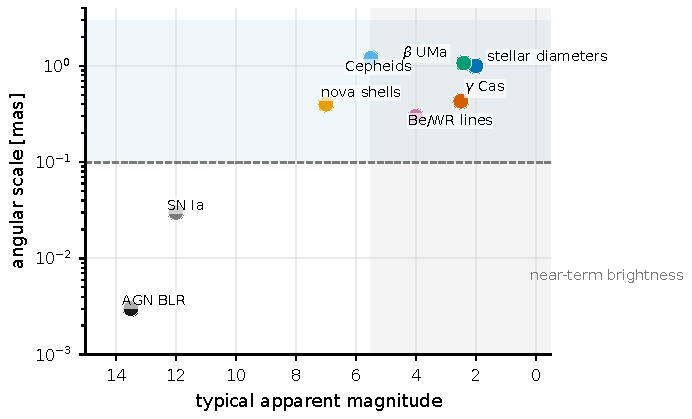
\includegraphics[width=0.88\linewidth]{figures/generated/chapter_19/ch19_science_case_feasibility.pdf}
\caption{第一代候选目标的亮度和角尺度位置。亮星角直径、\(\beta\) UMa、\(\gamma\) Cas 和 Be/WR 谱线区同时满足“够亮”和“能被百米级基线解析”；Type Ia、AGN BLR 和暗物质小尺度透镜科学价值高，但亮度、事件率或角尺度把它们推向长期项目。}
\label{fig:ch19-case-plane}
\end{figure}

一个实用排序分数可写成
\begin{equation}
  \mathcal P
  =
  \frac{
  W_{\rm sci}\,
  R_{\rm tech}\,
  R_{\rm prior}
  }{
  1+R_{\rm sys}+R_{\rm trigger}
  } .
  \label{eq:ch19-priority-score}
\end{equation}
\begin{formulaexplain}[公式 (19.1) 解读]
\(\mathcal P\) 是项目排序分数。科学回报、技术成熟度和外部先验提高分数；系统误差风险和触发风险降低分数，用来避免只凭“题目好听”选目标。
\end{formulaexplain}
\(W_{\rm sci}\) 是科学回报，\(R_{\rm tech}\) 是技术成熟度，\(R_{\rm prior}\) 是外部先验和模型可解释性，\(R_{\rm sys}\) 是系统误差风险，\(R_{\rm trigger}\) 是触发和调度风险。实际排序只需要粗分档，目的是防止单一维度支配选择。例如 Type Ia 几何距离的 \(W_{\rm sci}\) 很高，但 \(R_{\rm trigger}\) 和 \(R_{\rm tech}\) 也高；亮星角直径的 \(W_{\rm sci}\) 中等，却有很高 \(R_{\rm tech}\) 和低系统风险，适合做第一批验收指标 \citep{2025PhRvD.111h3047K,2024ApJ...966...28A,2024MNRAS.529.4387A}。

\section{恒星角直径、有效温度和快速自转为什么先做}

角直径是第一代最成熟的科学产品。观测量是 \(|V|^2(B,\lambda)\)，模型通常从均匀圆盘开始，再用 limb-darkened profile 或完整大气模型修正。角直径进入有效温度的方式很直接：
\begin{equation}
  F_{\rm bol}
  =
  \frac{\theta_{\rm LD}^2}{4}
  \sigma_{\rm SB}T_{\rm eff}^4,
  \qquad
  T_{\rm eff}
  =
  \left(
  \frac{4F_{\rm bol}}
  {\sigma_{\rm SB}\theta_{\rm LD}^2}
  \right)^{1/4}.
  \label{eq:ch19-teff}
\end{equation}
\begin{formulaexplain}[公式 (19.2) 解读]
\(F_{\rm bol}\) 是总辐射流量，\(\theta_{\rm LD}\) 是边缘昏暗角直径，\(T_{\rm eff}\) 是有效温度。角直径一旦测准，就能把流量转换成恒星温度尺度。
\end{formulaexplain}
\(F_{\rm bol}\) 是地球处总辐射流量，单位 \({\rm erg\,s^{-1}\,cm^{-2}}\)；\(\theta_{\rm LD}\) 是边缘昏暗角直径，单位 rad；\(\sigma_{\rm SB}\) 是 Stefan--Boltzmann 常数。若 \(\theta_{\rm LD}\) 误差为 \(4\%\)，只由角直径传播到 \(T_{\rm eff}\) 的误差约为 \(2\%\)。因此，亮星角直径重复测量不只是仪器复现实验；它会进入 \(T_{\rm eff}\)、半径、年龄、旋转模型和标准星尺度的校准 \citep{1967MNRAS.137..393H,1974MNRAS.167..121H,1977MNRAS.180..177B,1986Natur.323..234D,2003RPPh...66..789M}。

VERITAS-SII 已把这条路线推进到现代仪器。它对 \(\beta\) CMa 和 \(\epsilon\) Ori 给出亚毫角秒直径，并且比 Narrabri 用少得多的观测时间达到优于 \(5\%\) 的结果；后续 \(\beta\) UMa 观测在 416 nm 得到 limb-darkened 角直径 \(\theta_{\rm LD}=1.07\pm0.04_{\rm stat}\pm0.05_{\rm sys}\,{\rm mas}\)，与 CHARA 近红外和 Keck 中红外结果互相校验。MAGIC-SII 的升级系统报告了 22 个恒星直径，其中 9 个是参考星、13 个此前没有可比测量；强度干涉已经开始提供成批的角直径数据，而不再只是单次演示 \citep{2020NatAs...4.1164A,2024ApJ...966...28A,2024MNRAS.529.4387A}。

\Needspace{13\baselineskip}
快速自转星是角直径案例的自然升级。均匀圆盘只需要 \(\theta\)，椭圆 photosphere 至少需要短轴 \(\theta_{\rm min}\)、轴比 \(r=\theta_{\rm maj}/\theta_{\rm min}\) 和位置角 \(\varphi_\star\)。椭圆模型可以写成
\begin{equation}
  x_{\rm ell}
  =
  \frac{\pi B_p\theta_{\rm min}}{\lambda}
  \left[
  \cos^2\psi
  +
  r^2\sin^2\psi
  \right]^{1/2},
  \qquad
  |V_{\rm ell}|^2
  =
  \left[\frac{2J_1(x_{\rm ell})}{x_{\rm ell}}\right]^2 .
  \label{eq:ch19-elliptical-visibility}
\end{equation}
\begin{formulaexplain}[公式 (19.3) 解读]
\(x_{\rm ell}\) 是椭圆盘在当前投影基线上的无量纲空间频率，\(r\) 是轴比，\(\psi\) 是基线方向角。公式把快速自转星的扁形光球写成可拟合的 \(|V|^2\) 曲线。
\end{formulaexplain}
\(\psi\) 是投影基线相对短轴的角度。若基线位置角覆盖不足，\(r\) 和 \(\varphi_\star\) 会严重退化。VERITAS 对 \(\gamma\) Cas 的结果给出短轴角直径约 \(0.43\pm0.02_{\rm stat}\pm0.02_{\rm sys}\,{\rm mas}\)、轴比约 \(1.28\pm0.04\pm0.02\)、旋转轴位置角约 \(116^\circ\)，并用 Roche--von Zeipel 模型推断其接近 breakup rotation。第一代强度干涉已经能从“大小”推进到“形状”和“重力昏暗” \citep{2025ApJ...995..191A}。

\section{双星、Be 星盘和 Wolf-Rayet 风怎样用基线分开}

密近双星的好处是信号形状很有辨识度。两个未解析点源，角分离向量为 \({\bf s}\)，流量比为 \(f=F_2/F_1\)，则
\begin{equation}
  |V_{\rm binary}|^2
  =
  \left|
  \frac{1+f\,e^{-2\pi i{\bf u}\cdot{\bf s}}}
  {1+f}
  \right|^2
  =
  \frac{1+f^2+2f\cos(2\pi{\bf u}\cdot{\bf s})}
  {(1+f)^2}.
  \label{eq:ch19-binary-visibility}
\end{equation}
\begin{formulaexplain}[公式 (19.4) 解读]
\({\bf u}\) 是空间频率，\({\bf s}\) 是双星角分离，\(f\) 是流量比。指数相位带来随基线振荡的 \(|V|^2\)，所以强度干涉仍能约束双星分离。
\end{formulaexplain}
\({\bf u}={\bf B}_\perp/\lambda\)。当 \(f=1\) 时，\(|V|^2\) 会从 1 振荡到 0；当 \(f=0.1\) 时，振幅只有 \(2f/(1+f)^2\simeq0.17\)，对校准和 SNR 的要求高很多。双星项目最适合已有光谱轨道或食双星先验的系统；每个夜晚的少量基线点能被轨道模型连接起来，失败时也能给出分离或亮度比上限 \citep{1974MNRAS.167..121H,2012MNRAS.419..172N,2014MNRAS.437..798M,2022MNRAS.512.1722K}。

\begin{figure}[tbp]
\centering
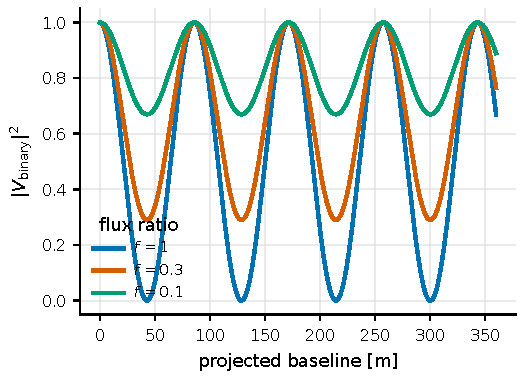
\includegraphics[width=0.82\linewidth]{figures/generated/chapter_19/ch19_binary_visibility.pdf}
\caption{1 mas 双星在 416 nm 下的平方可见度振荡。等亮双星给出深振荡；流量比降到 0.3 或 0.1 后，振荡振幅迅速变小。双星项目需要基线覆盖和轨道先验，否则亮度比、分离和位置角会互相退化。}
\label{fig:ch19-binary-visibility}
\end{figure}

\Needspace{12\baselineskip}
Be 星盘和 Wolf-Rayet 风把“空间分辨”与“谱线选择”连在一起。连续谱主要来自 photosphere，H\(\alpha\)、He 或 Fe 线可来自扩展盘、风碰撞区或 Weigelt blob 一类稠密结构。若谱线和连续谱混合，总可见度是通量加权和：
\begin{equation}
  V_{\rm obs}
  =
  \frac{
  F_{\rm c}V_{\rm c}
  +
  F_{\rm line}V_{\rm line}
  }{
  F_{\rm c}+F_{\rm line}
  } .
  \label{eq:ch19-line-continuum}
\end{equation}
\begin{formulaexplain}[公式 (19.5) 解读]
\(V_{\rm c}\) 和 \(V_{\rm line}\) 分别是连续谱和谱线区可见度，\(F_{\rm c}\) 与 \(F_{\rm line}\) 是对应通量。观测到的是通量加权平均，谱线几何必须和连续谱分开解释。
\end{formulaexplain}
\(F_{\rm line}/F_{\rm c}\) 可以从同时光谱或窄带/连续谱滤光片估计。若谱线区比 photosphere 大，长基线 \(|V_{\rm line}|^2\) 会比连续谱下降得更快；若谱线来自很小的高亮斑，长基线会保留信号。Narrabri 对 \(\gamma^2\) Velorum 的 WR 风已经展示了发射线区和连续谱区可以有不同角尺度；现代多基线阵列可把这一思想推广到 Be decretion disk、快速自转热星和相互作用双星 \citep{1970MNRAS.148..103H,2010SPIE.7734E..0AD,2012NewAR..56..143D,2025ApJ...995..191A}。

\section{新星、Type Ia 和可触发瞬变什么时候值得抢}

膨胀瞬变的几何关系简单，观测要求却很硬。若外壳以速度 \(v_{\rm exp}\) 近似自由膨胀，角直径为
\begin{equation}
  \theta(t)
  \simeq
  \frac{2v_{\rm exp}(t-t_0)}{D},
  \qquad
  D
  \simeq
  \frac{2v_{\rm exp}(t-t_0)}{\theta}.
  \label{eq:ch19-expansion}
\end{equation}
\begin{formulaexplain}[公式 (19.6) 解读]
\(\theta(t)\) 是膨胀外壳角直径，\(v_{\rm exp}\) 是膨胀速度，\(t_0\) 是爆发时刻，\(D\) 是距离。它是瞬变几何距离的最简账本。
\end{formulaexplain}
\(v_{\rm exp}\) 来自谱线速度，单位 \({\rm cm\,s^{-1}}\)；\(D\) 是距离；\(t-t_0\) 是爆发后时间。银河系新星在 \(D=2\,{\rm kpc}\)、\(v_{\rm exp}=10^8\,{\rm cm\,s^{-1}}\) 时，10 天后角直径已达数 mas，用百米以下基线即可解析；主要困难来自亮度演化、非球对称形状和尘埃。Type Ia 在 \(D=10\,{\rm Mpc}\)、\(v_{\rm exp}=10^9\,{\rm cm\,s^{-1}}\) 时，20 天后角直径只有 \(\sim0.02\,{\rm mas}\)，需要数 km 光学基线；限制它的主要是触发窗口、亮度和阵列规模 \citep{2025PhRvD.111h3047K}。

\begin{figure}[tbp]
\centering
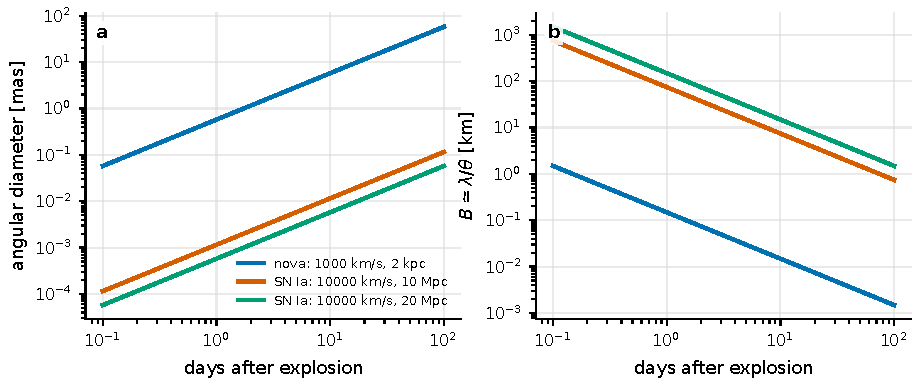
\includegraphics[width=0.94\linewidth]{figures/generated/chapter_19/ch19_transient_expansion.pdf}
\caption{膨胀瞬变的角直径和所需基线。银河系新星在几天到几十天内进入 mas 量级，适合第一代触发演练；10--20 Mpc 的 Type Ia 即使在峰值附近也只有几十微角秒量级，需要 km 级基线和 \(m\lesssim12\) 的近邻事件。}
\label{fig:ch19-transient-expansion}
\end{figure}

Type Ia 强度干涉几何距离是高回报长期目标。Kim 等的可行性研究把 \(m\lesssim12\) 作为可预见下一代观测的亮度范围，对应 \(z\sim0.004\) 的局部体积，预计全天每年约 1 个可用 Type Ia 量级事件。他们用辐射转移模型计算不同波长的表面亮度和 \(|V|^2\)，并指出光谱分辨可以提供多波长层析，测量对象不再局限于一个均匀圆盘半径。第一代项目可以从新星和近邻亮瞬变验证触发、滤光、背景和模型拟合流程；Type Ia 距离标尺应列为二代或专用阵列目标 \citep{2025PhRvD.111h3047K,1997A&A...320..799F,2004A&A...415..531S}。

\section{Crab 光子统计和自然激光怎样检验非热统计}

Crab pulsar 不是空间强度干涉的最佳目标，却是事件表科学的好目标。它亮、周期稳定、有精确星历，光学主脉冲和 interpulse 可以定义相位窗。相位误差为
\begin{equation}
  \Delta\phi
  =
  \frac{\Delta t}{P_{\rm spin}}.
  \label{eq:ch19-pulse-phase}
\end{equation}
\begin{formulaexplain}[公式 (19.7) 解读]
\(\Delta t\) 是时间戳误差，\(P_{\rm spin}\) 是脉冲星自转周期，\(\Delta\phi\) 是相位误差。时间精度越好，事件越能被放进正确的脉冲相位窗。
\end{formulaexplain}
Crab 的 \(P_{\rm spin}\simeq33\,{\rm ms}\)，\(1\,\mu{\rm s}\) 时间误差只对应 \(\Delta\phi\simeq3\times10^{-5}\)；毫秒脉冲星要求更严。AquEYE/Iqueye 这类仪器已经把光子以 ps 到 ns 级时间标签保存，适合做相位分辨 \(g^{(2)}\)、颜色相关或与射电 giant pulse 的条件叠加。Crab giant radio pulse 周期中的光学增强已经被测到，ARCONS 还显示早到的巨脉冲对应更强光学增强；第一代量子天文学可以把这些结果转成事件表统计和偏振/颜色分窗，不必停在平均光变曲线 \citep{2009JMOp...56..261B,2009A&A...508..531N,2015SPIE.9504E..0CZ,2003Sci...301..493S,2013ApJ...779L..12S}。

\begin{figure}[tbp]
\centering
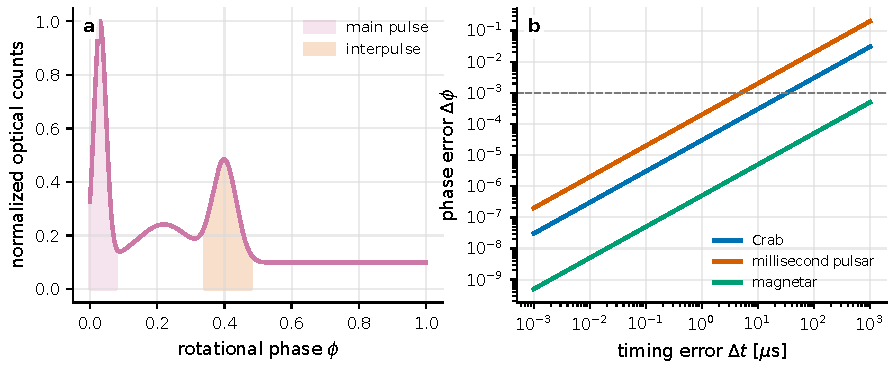
\includegraphics[width=0.94\linewidth]{figures/generated/chapter_19/ch19_crab_phase_windows.pdf}
\caption{Crab 型光学脉冲的相位窗和时间误差。左图示意主脉冲、bridge 和 interpulse 的事件选择；右图把时间误差转成相位误差。对 Crab，微秒级时间已经很宽裕；对毫秒脉冲星，ns--\(\mu\)s 级同步才保留窄相位结构。}
\label{fig:ch19-crab-phase}
\end{figure}

自然激光和受激辐射候选适合做“统计是否非热”的检验；一条亮谱线本身还不够。对 \(M\) 个互不相干热模式，
\begin{equation}
  g^{(2)}(0)-1
  =
  \frac{1}{M},
  \label{eq:ch19-mode-bunching}
\end{equation}
\begin{formulaexplain}[公式 (19.8) 解读]
\(M\) 是互不相干热模式数。模式越多，单模热光的聚束峰越被平均掉；因此 \(g^{(2)}(0)\) 接近 1 不必然说明光是理想激光。
\end{formulaexplain}
而理想相干态给 \(g^{(2)}(0)=1\)。未饱和 maser/laser、饱和放大、自发背景、多斑点叠加和仪器时间响应会产生不同统计。Eta Carinae 的 Weigelt blobs 中 Fe II 线被 Ly\(\alpha\) 泵浦，Johansson 和 Letokhov 讨论了 \(0.9-1.0\,\mu{\rm m}\) 和近红外 Fe II 激光线，线宽测量和 photon-correlation spectroscopy 可作为直接证据。若线宽为 \(\Delta\nu\)，相干时间约 \(\tau_c\sim1/(\pi\Delta\nu)\)；窄线会显著提升可解析相关 contrast，但也要求更高谱分辨、稳定滤光和严格的连续谱扣除 \citep{2004A&A...428..497J,2005NewA...10..361J,2008AIPC..984..216D}。

\begin{figure}[tbp]
\centering
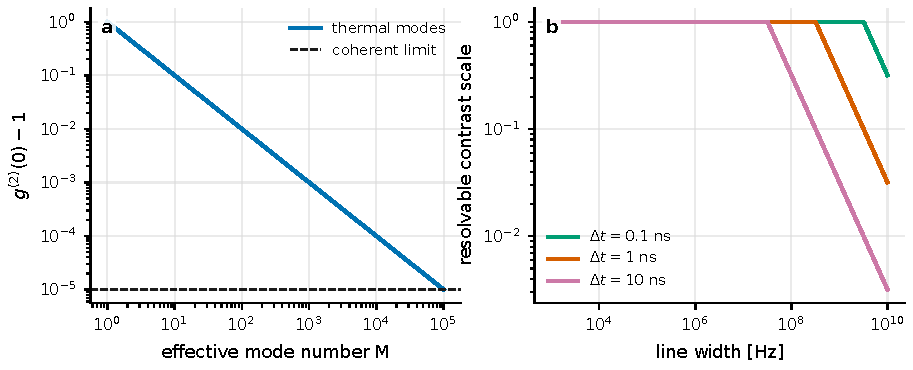
\includegraphics[width=0.94\linewidth]{figures/generated/chapter_19/ch19_natural_laser_statistics.pdf}
\caption{自然激光候选的两个统计量。左图显示热光模式数增加会把聚束峰压低，而相干极限接近 \(g^{(2)}(0)-1=0\)。右图显示线宽越窄，相干时间越长，在给定探测时间分辨率下越容易保留可解析 contrast。}
\label{fig:ch19-natural-laser}
\end{figure}

\section{第一代推荐顺序怎样随仪器成熟变化}

把这些案例放到同一矩阵里，第一代顺序主要由成熟度和系统风险决定。亮热星角直径、已知直径参考星、\(\beta\) UMa 类 A 型星，以及 MAGIC/VERITAS 可重复目标适合作为验收项目。\(\gamma\) Cas 类快速自转、Be/WR 谱线区、密近双星和新星早期膨胀是在同一套能力上继续增加科学信息。Crab 相位分辨统计和自然激光候选线更依赖事件表质量和时间/光谱筛选。Type Ia 几何距离、AGN BLR、暗物质小尺度透镜和量子网络辅助成像科学回报高，但更适合放在长期目标中。

\begin{figure}[!htbp]
\centering
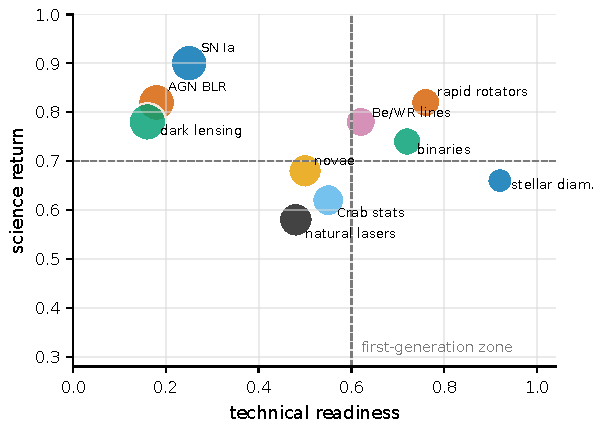
\includegraphics[width=0.78\linewidth]{figures/generated/chapter_19/ch19_priority_matrix.pdf}
\caption{第一代科学案例矩阵。横轴是技术成熟度，纵轴是科学回报，点越大表示系统误差和触发风险越高。右上方且点较小的目标最适合第一代验收；左上方目标科学价值高，但需要专用阵列或更成熟量子资源。}
\label{fig:ch19-priority}
\end{figure}

\begin{longtable}{p{0.17\linewidth}p{0.22\linewidth}p{0.23\linewidth}p{0.20\linewidth}}
\toprule
案例 & 第一观测量 & 典型数量级 & 第一代判据 \\
\midrule
亮星角直径 & \(|V|^2(B)\) & \(m_V<5\)，\(\theta=0.5-2\,{\rm mas}\) & 多夜重复到 \(3-5\%\) 直径精度。 \\
快速自转 & 多位置角 \(|V|^2\) & 轴比 \(1.1-1.5\)，\(\theta<1\,{\rm mas}\) & 能区分圆盘和椭圆模型。 \\
双星 & \(|V|^2\) 振荡 & 分离 \(0.2-5\,{\rm mas}\)，\(f>0.1\) & 已有轨道先验，覆盖两个以上位置角。 \\
Be/WR 谱线 & 谱线/连续谱 \(|V|^2\) & H\(\alpha\)、He、Fe 线 & 线通量足够，连续谱扣除可验证。 \\
新星 & \(\theta(t)\) & 几天后 mas 量级 & 触发快，能与谱线速度合并。 \\
Crab 统计 & 相位窗 \(g^{(2)}\) 和颜色相关 & \(P=33\,{\rm ms}\) & 星历、背景星云和绝对时间闭合。 \\
自然激光 & \(g^{(2)}\)、线宽、偏振 & \(\Delta\nu\) 可窄到高相干时间 & 谱线和连续谱可分离，有 null test。 \\
Type Ia & \(|V|^2(\lambda,t)\) & \(m<12\)，几十 \(\mu{\rm as}\) & km 级阵列和快速触发成熟后再做。 \\
\bottomrule
\end{longtable}

排序会随仪器状态改变。系统刚完成时间同步和零基线相关时，亮星角直径和参考星重复性最有价值；六条以上基线能稳定运行后，快速自转和双星进入主清单；窄带滤光和高数据吞吐可靠后，自然激光和谱线盘才开始有现实空间；阵列扩展到 km 级并能每年快速响应 \(m\lesssim12\) 的瞬变时，Type Ia 几何距离才会成为第一线科学目标 \citep{2017MNRAS.472.4126G,2022MNRAS.512.1722K,2024MNRAS.529.4387A,2024ApJ...966...28A,2025ApJ...995..191A,2025PhRvD.111h3047K}。


\chapter{教学实验和计算实验}
\label{chap:20}

\begin{chapteropening}
观测量、仪器响应和误差预算最终都要回到事件表。桌面 HBT、均匀圆盘拟合、双星可见度、事件表相关器、SPADE 模式排序和 Type Ia 超新星距离 toy model 表面上属于不同题目，输入却都是带时间、通道、偏振和质量标记的光子事件。本章的目标不是罗列几个可以运行的脚本，而是把每个案例都写成一条可检查的观测链：原始事件怎样变成统计量，统计量怎样带入物理模型，模型误差又怎样回到实验设计。HBT 的历史基础、量子光学教学实验、现代强度干涉仪器和模式测量分别见 \citet{1956Natur.178.1046H,1957RSPSA.242..300B,1963PhRv..130.2529G,1963PhRvL..10..277S,1985stop.book.....G,1995ocqo.book.....M,2002SPIE.4588..593L,2024arXiv240418606N,2009A&A...508..531N,2020NatAs...4.1164A,2016PhRvX...6c1033T,2025PhRvD.111h3047K}。
\end{chapteropening}

\section{事件表为什么是一切教学实验的共同语言}

课程的第一步应该让学生看到，事件表不是仪器工程里的琐碎文件格式，而是把光场随机性保留下来的最小记录。平均光变曲线只是事件表的一个投影；一旦先把事件粗分箱，后面就无法重新选择时间窗、通道、偏振、质量筛选或 time-shift 背景。因此实验从事件表开始，事件行采用第 \ref{chap:01} 章式 \eqref{eq:event-row} 的字段，并按第 \ref{chap:06} 章的仪器层要求加入探测器编号、质量标记和时间校正。文件头要写清时间单位是 ns、ps 还是 GPS/UTC 时间戳，探测器编号如何编码，光谱和偏振通道是否存在，质量标记如何记录死时间附近事件、云层、电子学饱和、异常基线或背景窗口。AQuEye、IquEye 和类似光子计数仪器把每个光子保留为时间标签，时间分辨率可到几十 ps，绝对时间通常要用 GPS、铷钟或 White Rabbit 一类同步系统约束到 ns 或亚 ns 量级 \citep{2015SPIE.9504E..0CZ,2016SPIE.9907E..0NZ,2013NIMPA.725..187J,2020RScI...91a3108W}。像 Timepix 这样的像素计数芯片说明，事件表也可以同时带空间位置、能量或到达时间信息 \citep{2007NIMPA.581..485L}。

\begin{figure}[tbp]
\centering
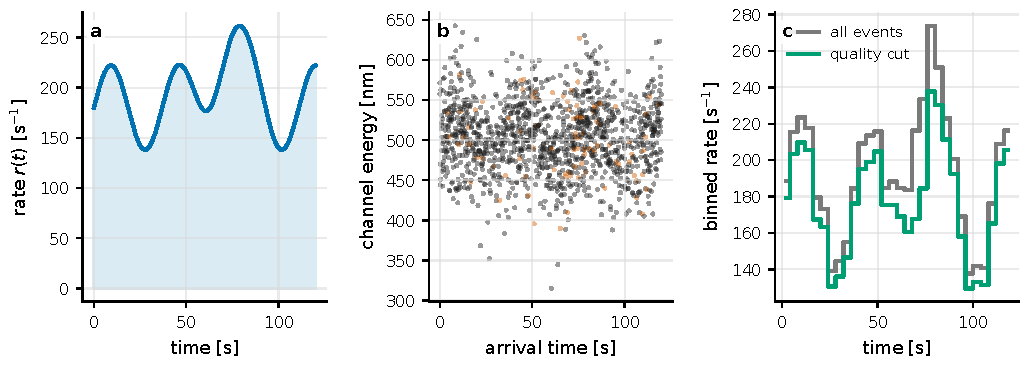
\includegraphics[width=0.96\linewidth]{figures/generated/chapter_20/ch20_event_table_simulation.pdf}
\caption{非齐次 Poisson 过程生成的模拟事件表。左图是输入光子率 \(r(t)\)，中图保留单个光子的到达时间、等效波长通道和质量标记，右图把事件表投影成光变曲线并显示质量筛选的影响。事件表比光变曲线多保留了通道和质量信息，因此同一份数据还能重新用于相关、偏振或能谱分析。}
\label{fig:chapter-20-event-table}
\end{figure}

把事件表投影成光变曲线是一种有损压缩，但它是最容易检查 Poisson 噪声和曝光变化的入口。如果只关心光变曲线，可以把事件表按时间 bin 投影：
\begin{equation}
  n_k = \sum_i {\bf 1}(t_i\in[t_k,t_k+\Delta t))\,{\bf 1}(q_i=1).
  \label{eq:ch20-binned-count}
\end{equation}
\begin{formulaexplain}[公式 (20.1) 解读]
\(n_k\) 是第 \(k\) 个时间 bin 中通过质量筛选的事件数。两个指示函数分别检查到达时间是否落入 bin、事件质量是否合格。
\end{formulaexplain}
\(n_k\) 是第 \(k\) 个 bin 的光子数，没有单位；\(\Delta t\) 是 bin 宽，桌面实验常取 ns 到 ms，天文计时可以从 ns 到分钟；\(q_i=1\) 表示通过质量筛选。估计光子率时 \(r_k=n_k/\Delta t\)，单位是 \({\rm s}^{-1}\)。当每个 bin 内的平均光子数小于几到几十个时，Poisson 噪声不能直接用高斯误差替代；当 \(n_k\gtrsim 30\) 时，高斯近似通常足够。未分箱 Poisson 点过程似然已经在式 \eqref{eq:ch07-point-process-likelihood} 中给出，分箱形式见式 \eqref{eq:ch07-binned-poisson}。同一份事件表既可以直接用事件时间拟合，也可以分箱成光变曲线拟合；两者的比较会显示快速变化和不均匀曝光怎样改变误差。这个形式也能解释为什么 Bayesian Blocks 等事件时间分割方法适合处理脉冲、耀发和强度干涉质量窗口 \citep{2013ApJ...764..167S}。

桌面 HBT 实验要回答的第一个问题是：两路强度各自随机，为什么零延迟附近会比远离零延迟略多一些共同起伏？热光或伪热光可以看成许多相位随机的模式叠加，瞬时强度会涨落；同一个相干时间内分到两个探测器的光子共享这一次强度涨落，所以符合数在 \(\tau=0\) 附近增加。激光直接照到两个探测器时 \(g^{(2)}(0)\simeq1\)，旋转毛玻璃产生的伪热光在单模极限下可以接近 \(g^{(2)}(0)=2\)，多模和有限时间响应会把峰压低 \citep{1991PhRvL..67.1426N,1996PhRvL..76.4344B,1999PhRvA..60..674B,2003PhRvL..91z2301A,2011PhRvL.107u7401C,2024arXiv240418606N}。延迟直方图和 \(g^{(2)}\) 归一化已经在式 \eqref{eq:ch07-pair-count} 和 \eqref{eq:ch07-g2-estimator} 中定义；教学实验要让学生亲手选择 \(\Delta\tau\)、time-shift 背景和质量筛选。若 \(R_1=R_2=5\times10^5\,{\rm s}^{-1}\)、\(T=300\,{\rm s}\)、\(\Delta\tau=0.5\,{\rm ns}\)，随机符合约为 \(3.75\times10^4\) pair/bin，shot-noise 相对误差约 \(1/\sqrt{H}\simeq5\times10^{-3}\)。这个数量级很直观：\(g^{(2)}-1\) 的 \(10^{-2}\) 峰可以在桌面上看见，而 \(10^{-5}\) 的天文聚束峰需要大面积望远镜、长积分和稳定背景。

\begin{figure}[tbp]
\centering
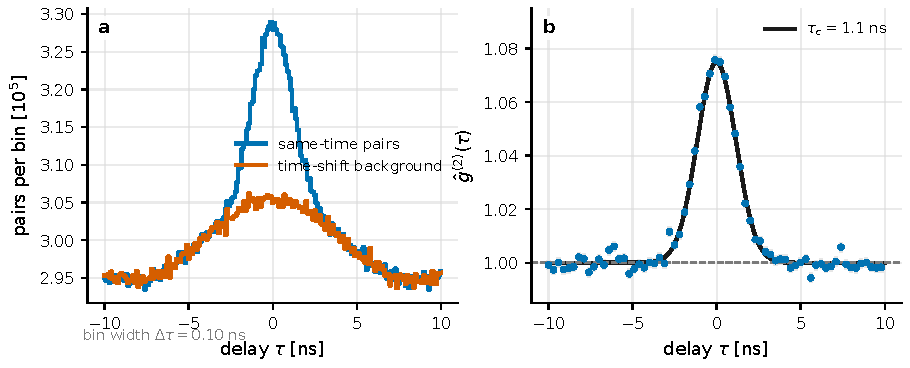
\includegraphics[width=0.96\linewidth]{figures/generated/chapter_20/ch20_hbt_lab_histogram.pdf}
\caption{桌面 HBT 实验的延迟直方图。左图比较同时时间轴的 pair/bin 和 time-shift 背景；慢漂移会同时出现在两条曲线中。右图用背景直方图归一化后得到 \(\hat g^{(2)}(\tau)\)，零延迟附近的峰宽由光源相干时间和探测器响应共同决定。}
\label{fig:chapter-20-hbt}
\end{figure}

真实仪器看到的相关函数是理想 \(g^{(2)}\) 被探测器时间响应卷积后的结果；响应卷积和 jitter budget 见式 \eqref{eq:ch06-response-convolution} 和 \eqref{eq:ch06-jitter-budget}。实验报告应给出响应核的测量方式，而不是只给最终的峰高。若相干时间 \(\tau_c\) 远小于时间 bin 或电子学响应宽度 \(\Delta t\)，热光峰的观测对比度近似按 \(\tau_c/\Delta t\) 稀释。可见光窄带滤光片若中心在 \(416\,{\rm nm}\)、带宽 \(13\,{\rm nm}\)，相干时间只有 \(4\times10^{-14}\,{\rm s}\) 量级；用几 ns 电子学采样时，聚束对比度自然落到 \(10^{-5}\) 量级。学生如果在桌面上只看到一个很漂亮的高峰，反而要追问它来自单模热光、电子串扰、光源慢漂移还是归一化选择。VERITAS、MAGIC 和 Asiago 光子计数实验的强度干涉分析都显式处理这个稀释、背景和死时间问题 \citep{2009A&A...508..531N,2009JMOp...56..261B,2017MNRAS.472.4126G,2020NatAs...4.1164A,2021MNRAS.506.1585Z,2022MNRAS.512.1722K,2024MNRAS.529.4387A,2024ApJ...966...28A}。

\section{桌面 HBT 怎样过渡到恒星角直径和双星}

把 HBT 从桌面搬到两台望远镜后，仍然不是把两处电场直接合束，而是比较两路强度起伏是否同步。区别在于，来自一个有角大小的天体时，两台望远镜接收到的热光涨落不再完全相同；基线越长，两个孔径看到的相干涨落越少，零延迟峰就越低。热光的 Siegert 关系已经在第 \ref{chap:04} 章式 \eqref{eq:ch04-siegert} 中给出，空间强度干涉形式见第 \ref{chap:05} 章式 \eqref{eq:ch05-hbt-spatial} 和 \eqref{eq:ch05-correlation-model}。\(\gamma_{12}\) 表示两台望远镜之间的一阶复相干度，\(|\gamma_{12}|^2\) 等同于天体亮度分布的归一化可见度平方；\(\beta\) 收集时间响应、光谱带宽、偏振选择和仪器效率造成的对比度稀释。若只用单个线偏振、\(\tau_c/\Delta t=10^{-5}\)，则 \(\beta\) 常在 \(10^{-6}\)--\(10^{-5}\) 量级。教学模拟可以故意取 \(\beta=0.05\) 让信号可见，但实验报告要把这个放大因子说清楚。

圆盘星最常用的模型是第 \ref{chap:05} 章式 \eqref{eq:ch05-uniform-disk} 的均匀圆盘，第一零点见式 \eqref{eq:ch05-first-null}。这个案例的教学重点是把每个符号都变成可测量的旋钮：\(\theta\) 是角直径，单位 rad、mas 或 \(\mu{\rm as}\)；\(B_\perp\) 是投影基线，单位 m；\(\lambda\) 是观测波长，单位 m；\(J_1\) 是一阶 Bessel 函数。在 \(\lambda=416\,{\rm nm}\) 时，\(\theta=1\,{\rm mas}\) 的第一零点约在 \(105\,{\rm m}\)。这就是为什么 VERITAS 这类百米级 Cherenkov 阵列可以测亮星角直径，而 Type Ia 超新星的几 \(\mu{\rm as}\) 角半径需要 km 级基线。

\begin{figure}[tbp]
\centering
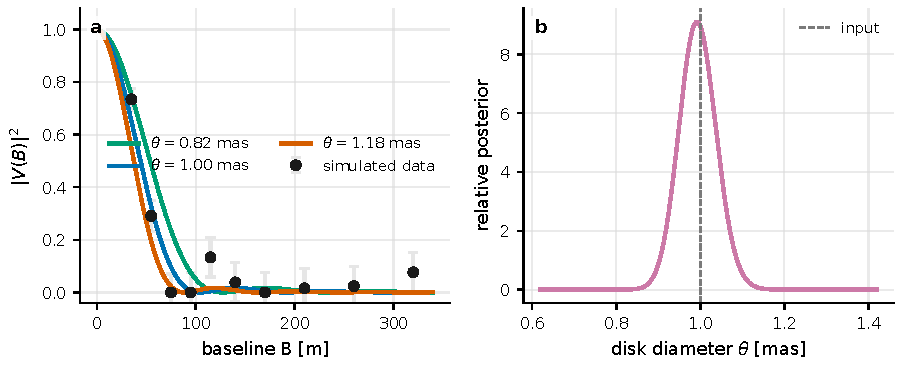
\includegraphics[width=0.96\linewidth]{figures/generated/chapter_20/ch20_uniform_disk_fit.pdf}
\caption{均匀圆盘强度干涉拟合。左图模拟 \(\lambda=416\,{\rm nm}\)、\(\theta=1\,{\rm mas}\) 目标在不同基线上的 \(|V|^2\) 测量；第一零点附近的斜率最大，对角直径最敏感。右图把这些数据转成角直径后验，后验宽度由 \(|V|^2\) 误差、基线覆盖和模型假设共同决定。}
\label{fig:chapter-20-uniform-disk}
\end{figure}

从数据估计 \(|V|^2\) 时，每条基线 \(b\) 先给出零延迟过量相关
\(\hat c_b=\hat g^{(2)}_b(0)-1\)。同夜标定星或实验室标定给出仪器对比度 \(\beta_b\)，于是
\begin{equation}
  \widehat{|V_b|^2}=\frac{\hat c_b}{\hat\beta_b}.
  \label{eq:ch20-v2-estimator}
\end{equation}
\begin{formulaexplain}[公式 (20.2) 解读]
\(\hat c_b\) 是基线 \(b\) 的零延迟相关超额，\(\hat\beta_b\) 是仪器对比度。两者相除才得到天体的 \(|V_b|^2\)，所以校准误差会被直接放大。
\end{formulaexplain}
\(\hat c_b\) 和 \(\hat\beta_b\) 都是无量纲量。若随机符合数为 \(H_b\)，且系统误差暂时忽略，\(\sigma_{\hat c}\simeq H_b^{-1/2}\)。\(\beta\) 一旦小到 \(10^{-5}\)，同样的 \(\sigma_{\hat c}\) 会被放大成 \(\sigma_{|V|^2}\simeq \sigma_{\hat c}/\beta\)。教学模拟若把 \(\beta\) 取得过大，会给出过于漂亮的 \(g^{(2)}\) 峰；天文 \(|V|^2\) 精度仍由真实对比度、随机符合数和系统地板决定。

双星模型让学生看到相位虽然在强度干涉中丢掉了符号，但空间频率振荡仍然保留下来。两点源的 \(|V|^2\) 形式在第 \ref{chap:10} 章式 \eqref{eq:ch10-binary} 和第 \ref{chap:19} 章式 \eqref{eq:ch19-binary-visibility} 已经写出；案例只需把通量比 \(\rho=F_2/F_1\)、角分离向量 \(\boldsymbol s\) 和投影相位 \(2\pi\boldsymbol B_\perp\cdot\boldsymbol s/\lambda\) 放进模拟。 \(\boldsymbol s\) 用 rad 表示，实际写报告常用 mas；\(\boldsymbol B_\perp\cdot\boldsymbol s/\lambda\) 是无量纲相位。等亮双星 \(\rho=1\) 的振荡可以从 1 降到 0；若伴星只有主星 \(10\%\) 的通量，振荡深度约为 \(0.17\)。在 \(B=180\,{\rm m}\)、\(\lambda=500\,{\rm nm}\) 时，\(0.5\,{\rm mas}\) 分离对应相位约 \(5.5\)，单条基线已经能看到明显振荡。轨道拟合时，\(\boldsymbol s(t)\) 随时间变，固定基线也会扫过不同相位。

\begin{figure}[tbp]
\centering
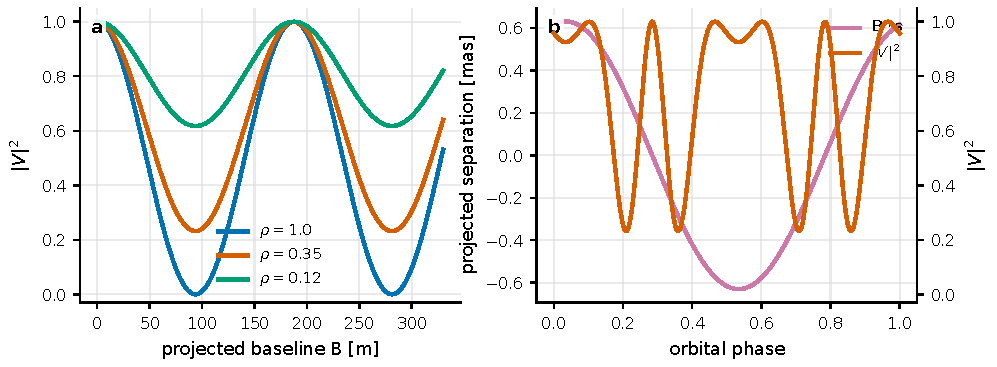
\includegraphics[width=0.96\linewidth]{figures/generated/chapter_20/ch20_binary_visibility.pdf}
\caption{双星 \(|V|^2\) 案例。左图显示固定角分离下通量比 \(\rho\) 如何控制基线振荡深度；右图显示倾斜轨道中投影分离 \(\boldsymbol B\cdot\boldsymbol s\) 随轨道相位变化，并改变固定基线上的 \(|V|^2\)。多基线和多历元数据用来分开分离、通量比和轨道几何。}
\label{fig:chapter-20-binary}
\end{figure}

\section{相关器怎样把事件表变成可检验的相关函数}

相关器案例不要一开始就变成软件性能比赛。先让学生用最朴素的方法确认：相关器的任务是把事件表变成一批延迟直方图或协方差估计；每一个 pair 都必须能追溯到两条原始事件和一个时间差。最朴素的双重循环需要比较所有事件对，计算量随 \(N_1N_2\) 增长；若事件已经按时间排序，只需要比较落在相关窗口 \(|t_j-t_i|<\tau_{\max}\) 内的邻近事件，计算量约为 \(N_\gamma k\)，其中 \(k\sim2R\tau_{\max}\) 是每个事件附近的候选事件数。把事件投影到均匀时间 bin 后，也可以用 FFT 做互相关，计算量约为 \(M\log M\)，\(M=T/\Delta t\)。三种方法估计的是同一个量，但内存、时间 bin 和死时间处理方式不同。

多望远镜阵列的基线数按第 \ref{chap:05} 章式 \eqref{eq:ch05-baseline-number} 随 \(N_{\rm tel}^2\) 增长：4 台望远镜只有 6 条基线，60 台望远镜有 1770 条基线。单望远镜原始数据率的估算见第 \ref{chap:06} 章式 \eqref{eq:ch06-data-rate}；\(\Delta t=4\,{\rm ns}\)、\(N_\nu=1\)、\(n_{\rm bit}=16\) 时，\(D\simeq4\,{\rm Gb\,s^{-1}}\)。若同时保留 64 个光谱通道，单望远镜就到 \(256\,{\rm Gb\,s^{-1}}\)。这解释了为什么现代强度干涉需要 GPU/FPGA 实时相关、分层触发、片上累加或严格的数据压缩；MAGIC 的实时无死时间相关器和 VERITAS 的离线/在线流程都是围绕这个数据率压力设计的 \citep{2020NatAs...4.1164A,2024MNRAS.529.4387A,2024ApJ...966...28A}。

\begin{figure}[tbp]
\centering
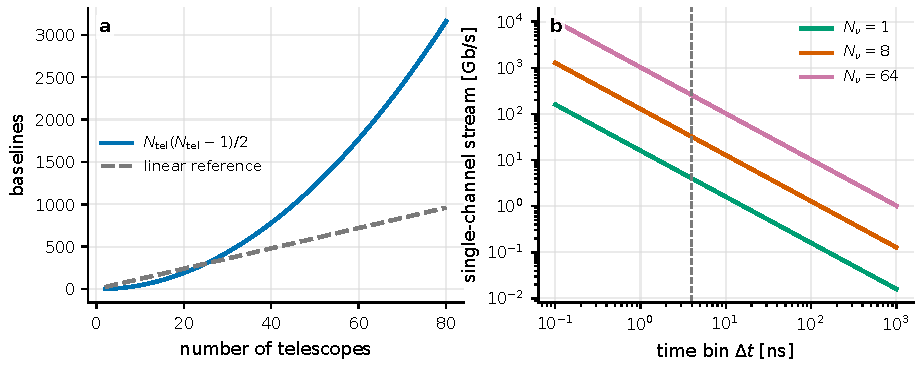
\includegraphics[width=0.96\linewidth]{figures/generated/chapter_20/ch20_correlator_scaling.pdf}
\caption{多望远镜相关器的两个标度。左图显示基线数随望远镜数二次增长，因此阵列扩展会迅速增加相关任务数量。右图显示单路数据流随时间 bin 变窄和光谱通道增多而上升；ns 级采样和几十个光谱通道已经进入需要实时硬件或 GPU 处理的区域。}
\label{fig:chapter-20-correlator}
\end{figure}

相关器案例要包含 null test，而且 null test 应该像结果图一样被评分。把第二路事件整体平移远大于 \(\tau_c\) 的时间后，真实峰应消失；在没有星光或用遮光片时运行同样流程，电子学串扰不应产生零延迟峰；把偏振或光谱通道打乱后，只有物理上应相关的通道保留信号；把数据按时间切片时，\(\hat g^{(2)}(0)-1\) 应随积分时间按 \(T^{-1/2}\) 收敛，而非集中在某一小段。Guerin 等人的实验、AQuEye/IquEye 的光子计数方案以及现代 Cherenkov 阵列强度干涉都说明，这些质量控制直接决定结果能否解释 \citep{2017MNRAS.472.4126G,2016SPIE.9907E..0NZ,2020NatAs...4.1164A,2021MNRAS.506.1585Z,2024MNRAS.529.4387A}。

\section{Rayleigh curse 和 SPADE 教会学生什么}

这一节不是从强度干涉跳到另一个无关主题，而是用一个可计算例子强调同一条思想：仪器记录的默认图像不一定把待估参数的信息放在最显眼的像素里。直接成像用焦平面像素强度估计两点源分离。两个等亮非相干点源的分离 \(s\) 远小于点扩散函数宽度 \(\sigma\) 时，图像几乎只变宽一点点；像素强度对 \(s\) 的导数趋近于零，所以 Fisher 信息下降。这是 Rayleigh curse 在统计上的含义。量子估计理论指出，信息并没有在光场里消失，而是藏在合适的空间模式中 \citep{2015Optic...2..646T,2016PhRvX...6c1033T,2016OExpr..24.3684N,2017PhRvL.118g0801T}。

对高斯点扩散函数和等亮双点源，理想 Hermite--Gaussian 模式排序的概率分布已在第 \ref{chap:08} 章式 \eqref{eq:ch08-spade-probability} 给出。计算实验把 \(n=0,1,2,\ldots\) 当作横向模式编号，并保证分离 \(s\) 和 PSF 宽度 \(\sigma\) 用同一角单位或同一焦平面长度单位。若 \(s=0.2\sigma\)，则控制高阶模式权重的无量纲量为 \(2.5\times10^{-3}\)，绝大多数光子仍在 \(n=0\) 模式，但 \(n=1\) 的小概率变化对 \(s\) 很敏感。理想 SPADE 对分离的 Fisher 信息在 \(s\to0\) 时保持有限；直接像素成像则趋向零。实验上，模式错配、中心定位误差、像差和背景会引入信息地板，所以教学代码应该加入一个可调的模式串扰参数，不宜只画理想曲线。

\begin{figure}[tbp]
\centering
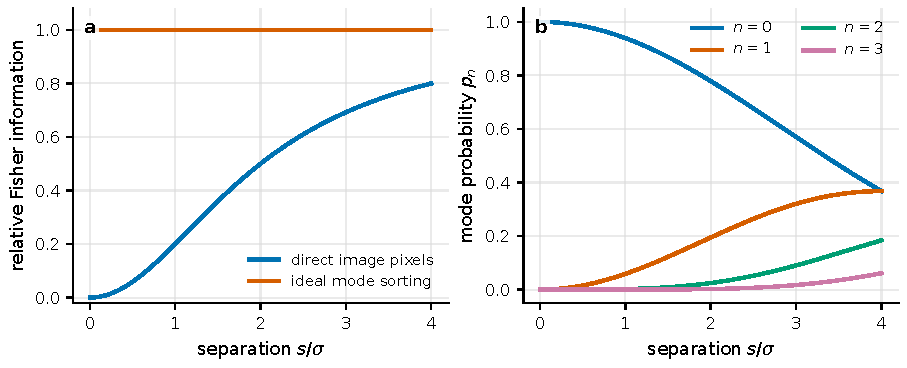
\includegraphics[width=0.96\linewidth]{figures/generated/chapter_20/ch20_spade_computational_experiment.pdf}
\caption{SPADE 计算实验。左图比较小分离处直接像素成像和理想模式排序的相对 Fisher 信息；直接成像在 \(s/\sigma\ll1\) 时信息下降，而模式排序保持接近常数。右图显示 Hermite--Gaussian 模式概率，分离很小时高阶模式概率很小但斜率非零，因此需要高稳定性和低串扰的模式测量。}
\label{fig:chapter-20-spade}
\end{figure}

这个案例和强度干涉指向同一件事：传统图像分辨率不是所有参数的信息极限。强度干涉用 \(|V|^2\) 访问长基线空间频率；SPADE 用模式投影访问直接图像中不显眼的分离信息。实际天文系统会同时面对弱光极限、背景光、多模混合、湍流、像差和探测器效率，因此模式排序更适合作为计算实验和 pathfinder，而不是直接承诺下一代望远镜可以无损达到量子极限。

\section{Type Ia 距离 toy model 怎样串起整套误差预算}

Type Ia 超新星项目把前面几个案例合在一起，也故意暴露最容易被 toy model 掩盖的危险：角半径、速度和爆炸时间看似只差一个比例常数，真实误差却来自不同仪器、不同模型和不同历元。光谱模型给出光球速度 \(v_{\rm ph}(t)\)，强度干涉给出角半径 \(\theta_{\rm ph}(t)\)，二者合成角直径距离：
\begin{equation}
  \theta_{\rm ph}(t)=\frac{R_{\rm ph}(t)}{D_A}
  \simeq \frac{v_{\rm ph}(t-t_0)}{D_A}.
  \label{eq:ch20-typeia-theta}
\end{equation}
\begin{formulaexplain}[公式 (20.3) 解读]
\(\theta_{\rm ph}\) 是光球角半径，\(R_{\rm ph}\) 是物理半径，\(D_A\) 是角直径距离。用速度和时间估计半径，再与角半径比较，就能约束距离。
\end{formulaexplain}
\(v_{\rm ph}\) 的单位是 \({\rm cm\,s^{-1}}\)，正常 Type Ia 在早期常为 \(8\times10^8\)--\(1.5\times10^9\,{\rm cm\,s^{-1}}\)；\(t-t_0\) 的单位是 s 或 d，强度干涉最感兴趣的是爆炸后几天到几十天；\(D_A\) 用 Mpc 表示；\(\theta_{\rm ph}\) 通常是几 \(\mu{\rm as}\) 到几十 \(\mu{\rm as}\)。例如 \(v_{\rm ph}=10^9\,{\rm cm\,s^{-1}}\)、\(t-t_0=15\,{\rm d}\)、\(D_A=20\,{\rm Mpc}\) 时，角半径约 \(4.3\,\mu{\rm as}\)。在 \(\lambda=500\,{\rm nm}\) 下，\(\lambda/\theta\) 对应 \(24\,{\rm km}\) 量级；若利用可见度曲线而不只等第一零点，km 到十 km 级基线仍然有科学信息，但误差预算会非常紧 \citep{2025PhRvD.111h3047K}。

距离后验可以用
\begin{equation}
  \ln{\cal L}(D_A)=
  -\frac{1}{2}\sum_k
  \left[
  \frac{\hat\theta_k-v_{{\rm ph},k}(t_k-t_0)/D_A}
  {\sigma_{\theta,k}}
  \right]^2
  -\frac{1}{2}\sum_k
  \left[
  \frac{\hat v_k-v_{{\rm ph},k}}
  {\sigma_{v,k}}
  \right]^2 .
  \label{eq:ch20-typeia-likelihood}
\end{equation}
\begin{formulaexplain}[公式 (20.4) 解读]
\(D_A\) 是待估距离，\(\hat\theta_k\) 和 \(\hat v_k\) 是第 \(k\) 个历元的角半径与速度观测。似然同时惩罚角半径和速度模型的不一致。
\end{formulaexplain}
\(\hat\theta_k\) 来自第 \(k\) 个历元的 \(|V|^2\) 拟合，单位是 \(\mu{\rm as}\) 或 rad；\(\hat v_k\) 来自光谱线速度或辐射转移模型，单位是 \({\rm cm\,s^{-1}}\)；\(\sigma_{\theta,k}\) 和 \(\sigma_{v,k}\) 分别包括统计误差和模型系统误差。这个 toy model 里若只给 \(\theta\) 加 \(10\%\) 噪声，会得到过于乐观的距离；完整项目还要让学生改变爆炸时间 \(t_0\)、速度梯度、非球对称和亮度分布模型，观察后验怎样变宽。

\begin{figure}[tbp]
\centering
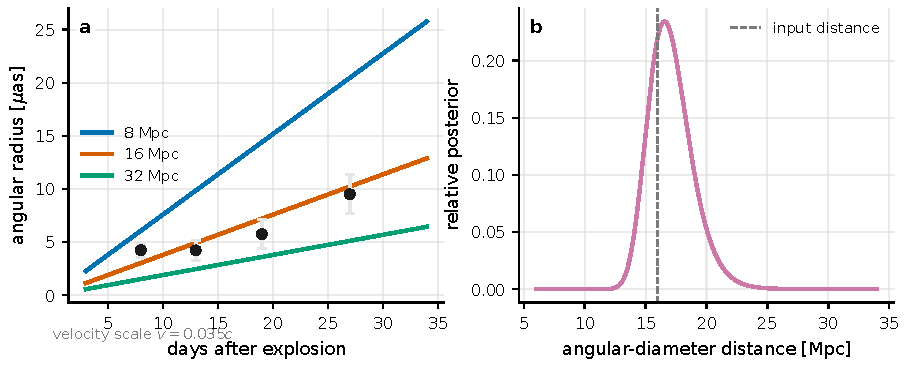
\includegraphics[width=0.96\linewidth]{figures/generated/chapter_20/ch20_typeia_distance_posterior.pdf}
\caption{Type Ia 超新星角直径距离 toy model。左图用 \(v_{\rm ph}=0.035c\) 的简化膨胀模型给出不同距离下的角半径随时间变化，并叠加模拟角半径测量；右图把这些角半径和速度模型合成 \(D_A\) 后验。真实分析需要用辐射转移模型替代常速度球壳，并把非球对称、谱线形成层和基线覆盖写入误差预算。}
\label{fig:chapter-20-typeia}
\end{figure}

课程项目可以按难度递进。最基础的实验用 LED、伪热光和激光测 \(g^{(2)}(\tau)\)，报告 \(R_1,R_2,T,\Delta\tau,\tau_c\) 和响应核 \(K\)。随后用同一份事件表实现 time-shift 背景、质量筛选和 \(T^{-1/2}\) 收敛测试。进入空间相干后，可以拟合均匀圆盘和双星 \(|V|^2\)，比较基线覆盖对 \(\theta\)、\(\rho\) 和 \(\boldsymbol s\) 的影响。更偏信息理论的项目实现 SPADE 概率和 Fisher 信息，并加入模式串扰和中心定位误差。综合项目可以做 Type Ia 距离 toy model，把角半径、速度和爆炸时间的不确定性一起传播。每个项目的产出包括一份事件表说明、一个 Python 脚本、一组 PDF 图、一个引用 ADS bib key 的短报告，以及至少两个 null test。

代码能运行只是第一关。时间相关项目需要说明时间基准、bin 宽、死时间、暗计数和随机符合估计；空间相干项目需要说明 \(B_\perp\)、\(\lambda\)、\(\beta\)、\(|V|^2\) 标定和源模型；模式测量项目需要说明点扩散函数宽度、模式基、串扰矩阵和背景；距离项目需要说明角半径估计、速度模型、爆炸时间和系统误差。缺少这些量时，图仍然可以生成，但结果不能当作天文测量。


\chapter{常见误区}
\label{chap:21}

\begin{chapteropening}
“单光子”“纠缠”“超分辨”“非 Poisson”“新物理”这些词很容易把问题说得过大。数据本身要更具体：事件表怎样变成联合概率，相关峰怎样标定，假警报怎样计算，模型参数在哪些条件下还能估计。本章按同一诊断顺序展开：先指出容易误读的说法，再写出真正的观测量，最后给出校准项、系统误差或 trial factor。量子光学的基本判据、强度干涉的天文实现、SPADE 的信息极限、天体 maser/laser 和天文统计检验分别见 \citet{1963PhRv..130.2529G,1963PhRvL..10..277S,1965RvMP...37..231M,1977PhRvL..39..691K,1985stop.book.....G,1995ocqo.book.....M,1956Natur.178.1046H,1957RSPSA.242..300B,1974iiia.book.....H,2020NatAs...4.1164A,2016PhRvX...6c1033T,1992ARA&A..30...75E,1979ApJ...228..939C,2013ApJ...764..167S}。
\end{chapteropening}

\section{看到光子为什么不等于量子天文学}

单光子探测器只是数据入口。若分析只把第 \ref{chap:01} 章式 \eqref{eq:event-row} 的事件表求和成平均计数率 \(R=N_\gamma/T\)，得到的仍然是普通光变曲线。量子天文学中新增的信息来自事件之间的联合分布，最简单的独立情形、二阶相关和 pair count 已在第 \ref{chap:02} 章式 \eqref{eq:ch02-independent} 和 \eqref{eq:ch02-g2-count} 中建立。判断一个分析是否用到了事件表，要看标签有没有进入模型：\(t\) 是到达时间，单位 s 或 ns；\(d\) 是探测器/望远镜编号；\(\nu\) 是频率通道，单位 Hz 或通道号；\(p\) 是偏振标签。若这些标签在分析时全部被丢掉，仅凭探测器能数单光子还不足以声称测到了新的量子观测量。

一个常见错误是把“低光子数”直接等同于“量子”。X 射线和伽马射线天文学长期使用 Poisson 计数和 Cash 似然，但许多问题仍只是平均强度或能谱估计 \citep{1979ApJ...228..939C,1986ApJ...303..336G}。反过来，射电和毫米波常处在高占有数、近经典波动极限，却仍能讨论相干函数、相位、偏振和量子噪声。判据在于模型是否需要多光子联合概率或光场模式来表达。

事件表也不会自动产生新物理。Poisson 计数模型已经在第 \ref{chap:01} 章式 \eqref{eq:poisson} 给出，分箱版本见第 \ref{chap:07} 章式 \eqref{eq:ch07-binned-poisson}。\(\mu_k=R_k\Delta t_k\) 是第 \(k\) 个 bin 的期望计数，没有单位。若源本来在变，\(\mu_k\) 也随时间变；若有效曝光 \(E_k\) 因云、死时间或选择函数改变，\(\mu_k\) 应写成 \(R_kE_k\Delta t_k\)。把所有 \(N_k\) 和一个常数 \(\mu\) 比较，然后宣布“非 Poisson”，通常只是把普通光变、坏天气或曝光变化误当作统计异常。Bayesian Blocks、周期搜索和似然比检验都能处理这类问题，但每种方法有自己的适用条件和试验次数 \citep{1982ApJ...263..835S,1992ApJ...398..146G,2002ApJ...571..545P,2013ApJ...764..167S}。

\section{\texorpdfstring{为什么 \(g^{(2)}=1\)}{为什么 g2=1} 不是充分判据}

\(g^{(2)}(0)=1\) 常被误说成“光一定是经典激光”，或者反过来被误说成“没有量子性”。相干态给 Poisson 光子数分布和 \(g^{(2)}(0)=1\)，但 \(g^{(2)}(0)=1\) 不是相干态的唯一指纹。多模热光在模式数 \(M\) 很大时也会接近 1；有限时间响应还会继续稀释聚束峰。对比度稀释的基本形式见第 \ref{chap:04} 章式 \eqref{eq:ch04-contrast-dilution}。\(\tau_c\) 是相干时间，单位 s；\(\Delta t_{\rm eff}\) 是探测器响应或相关 bin 的有效宽度，单位 s；有效模式数 \(M_{\rm eff}\) 包括空间、频率、偏振和时间模式。可见光 \(10\,{\rm nm}\) 带宽在 \(500\,{\rm nm}\) 附近给 \(\tau_c\sim10^{-14}\,{\rm s}\)，而电子学 bin 常是 \(10^{-9}\)--\(10^{-8}\,{\rm s}\)。即使 \(M_{\rm eff}=1\)，对比度也只有 \(10^{-6}\)--\(10^{-5}\)。Guerin 的星光聚束实验、AQuEye/IquEye 方案和 VERITAS/MAGIC 强度干涉都把这个稀释作为核心量处理 \citep{2017MNRAS.472.4126G,2016SPIE.9907E..0NZ,2020NatAs...4.1164A,2021MNRAS.506.1585Z,2024MNRAS.529.4387A,2024ApJ...966...28A}。

\begin{figure}[tbp]
\centering
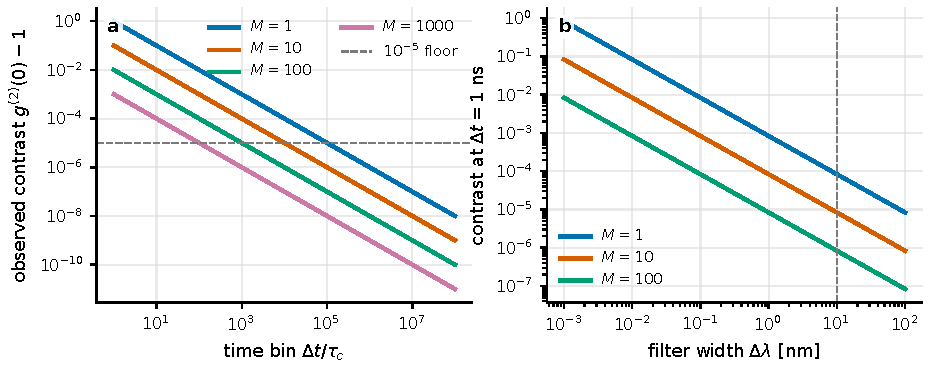
\includegraphics[width=0.96\linewidth]{figures/generated/chapter_21/ch21_g2_scaling_mistake.pdf}
\caption{时间 bin、光谱带宽和模式数对 \(g^{(2)}\) 对比度的稀释。左图显示 \(\Delta t/\tau_c\) 和 \(M_{\rm eff}\) 如何把单模热光的聚束峰压低；虚线表示 \(10^{-5}\) 级系统误差地板。右图把滤光片带宽换成相干时间，在 \(1\,{\rm ns}\) 采样下，宽带可见光的热光峰很容易低于可校准范围。}
\label{fig:ch21-g2-scaling}
\end{figure}

反聚束比 \(g^{(2)}=1\) 更强，因为 \(g^{(2)}(0)<1\) 不能由经典随机强度给出。Kimble、Dagenais 和 Mandel 的共振荧光实验是这个判据的经典例子 \citep{1977PhRvL..39..691K}。天体光源中要看到反聚束极难：光源通常由大量独立发射体、传播路径和探测器响应混合，任何单个量子发射体的亚 Poisson 特征都会被空间、频率和时间平均稀释。因此天文报告若写“\(g^{(2)}\simeq1\)，所以是激光”或“\(g^{(2)}\simeq1\)，所以没有量子信息”，都没有足够依据。

\section{强度干涉为什么仍然需要校准}

强度干涉对大气 piston 相位不敏感，但校准仍然决定相关幅度。透明度、闪烁、镜面反射率、滤光片形状、光电倍增管增益、SPAD 死时间、电子串扰和背景光都会进入相关幅度。一个实用的数据模型可以写成
\begin{equation}
  \hat c_b(\tau)=
  \beta_b\,|V_b|^2\,h_b(\tau)
  +c_{{\rm inst},b}(\tau)
  +c_{{\rm sel},b}(\tau)
  +\epsilon_b(\tau).
  \label{eq:ch21-calibration-model}
\end{equation}
\begin{formulaexplain}[公式 (21.1) 解读]
\(\hat c_b\) 是实测相关超额。第一项是天体信号，后面依次是仪器项、选择项和随机误差；强度干涉不怕大气相位，却仍怕这些幅度校准项。
\end{formulaexplain}
\(\hat c_b=\hat g_b^{(2)}-1\) 是基线 \(b\) 上的归一化相关超额；\(\beta_b\) 是零基线对比度或仪器稀释因子；\(|V_b|^2\) 是天体可见度平方；\(h_b(\tau)\) 是归一化峰形；\(c_{\rm inst}\) 是电子学和探测器项；\(c_{\rm sel}\) 是选择函数、天气和背景处理造成的项；\(\epsilon\) 是随机误差。所有项都是无量纲相关幅度。VERITAS 在拟合恒星角直径时显式处理背景光和零基线相关，MAGIC 的实时相关器则围绕连续记录、低串扰和快速模式切换设计 \citep{2020NatAs...4.1164A,2024MNRAS.529.4387A,2024ApJ...966...28A}。

\begin{figure}[tbp]
\centering
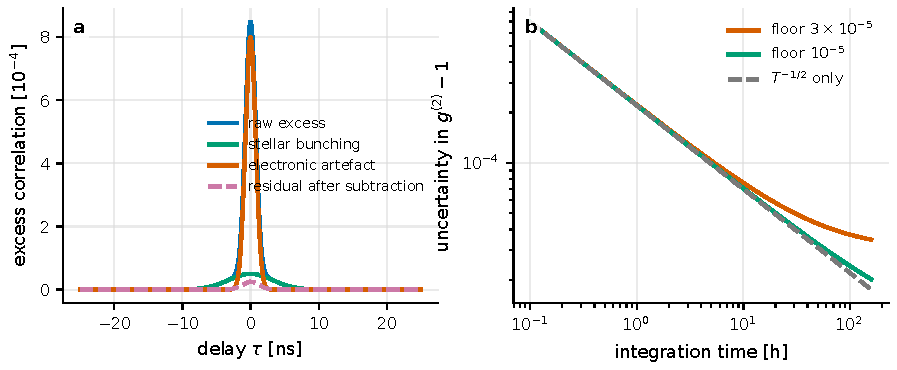
\includegraphics[width=0.96\linewidth]{figures/generated/chapter_21/ch21_calibration_artifacts.pdf}
\caption{校准误差怎样伪装成相关信号。左图中电子串扰峰比 \(5\times10^{-5}\) 的天体聚束峰大一个数量级以上，若模板扣除后还留下窄残差，就会污染 \(\hat g^{(2)}(0)\)。右图显示积分时间只按 \(T^{-1/2}\) 压低统计误差；一旦存在 \(10^{-5}\)--\(3\times10^{-5}\) 的系统误差地板，继续积分不能自动改善结论。}
\label{fig:ch21-calibration}
\end{figure}

Null test 要覆盖时间、空间、通道和积分行为。time-shift 把一路事件整体平移远大于仪器响应和天体相关宽度的时间，天体峰应消失，而慢漂移和背景结构应保留。off-source 或 off-band 换到无星光位置或不含目标谱线的频段，零延迟峰不应保留。通道置换把不应相关的探测器、偏振或光谱通道交叉相关，若仍有峰，优先怀疑串扰。分块收敛把数据按时间分成多段，相关幅度的均值应稳定，误差应按近似 \(T^{-1/2}\) 下降，直到系统地板出现。Guerin 的实验报告中，TDC 伪相关若不扣除会让 SNR 饱和；AQuEye/IquEye 文献也明确列出 SPAD 死时间、光纤延迟和环境控制对系统误差的影响 \citep{2017MNRAS.472.4126G,2016SPIE.9907E..0NZ,1996ApOpt..35.1956C,2013NIMPA.725..187J,2020RScI...91a3108W}。

\section{没有相位为什么不等于不能成像}

另一个误区是“强度干涉没有相位，所以只能测直径，不能成像”。复可见度的 Fourier 定义见第 \ref{chap:05} 章式 \eqref{eq:ch05-vcz}；强度干涉直接测的是 \(|V(u,v)|^2\)，确实丢掉了一阶复可见度相位。但 \(|V|^2\) 仍含有大量结构信息。均匀圆盘、边缘昏暗、双星、旋转扁星和简单盘面都可以直接用 \(|V|^2\) 拟合。主要困难来自退化和镜像。镜像亮度 \(I(-\boldsymbol\theta)\) 的可见度是 \(V^\ast(\boldsymbol u)\)，因此 \(|V|^2\) 完全相同；第 \ref{chap:05} 章图 \ref{fig:ch05-phase-ambiguity} 已经画出这个相位缺失问题。要分开镜像、非对称结构和复杂形态，需要多基线覆盖、物理先验、正则化 phase retrieval，或三阶相关等高阶信息 \citep{2003RPPh...66..789M,2009A&A...507.1719F,2012NewAR..56..143D,2014MNRAS.437..798M,2022MNRAS.512.1722K}。

\begin{figure}[tbp]
\centering
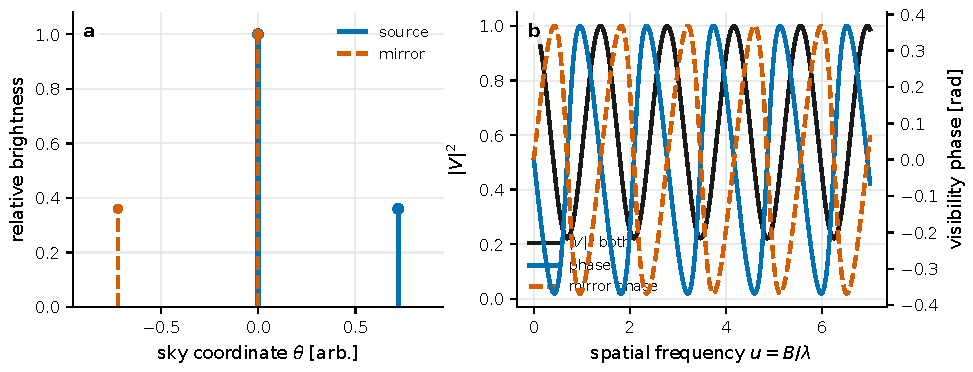
\includegraphics[width=0.96\linewidth]{figures/generated/chapter_21/ch21_phase_loss.pdf}
\caption{只测 \(|V|^2\) 的镜像退化。左图是一个不等亮双源和它的镜像；右图显示二者的 \(|V|^2\) 完全相同，但可见度相位符号相反。强度干涉可以约束结构，但需要多基线、模型先验或高阶相关来补回丢失的方向信息。}
\label{fig:ch21-phase-loss}
\end{figure}

三阶强度相关可在理想情况下给出类似闭合相位的信息，但信号比二阶相关更弱。若二阶相关的统计误差已经接近系统地板，三阶相关也会被同一批光子率和校准问题限制。大型阵列和极亮目标可以探索这个方向；第一代科学案例通常更适合从 \(|V|^2\) 的少参数模型开始，再逐步加入先验成像。

\section{量子超分辨为什么不能任意突破衍射}

SPADE 和相关模式测量纠正的是一个统计误解：Rayleigh 判据不是所有参数估计问题的信息极限。对两个弱、等亮、非相干点源，直接成像在 \(s/\sigma\ll1\) 时分离 Fisher 信息下降，而理想模式排序能保持有限 Fisher 信息 \citep{2015Optic...2..646T,2016PhRvX...6c1033T,2016OExpr..24.3684N,2017PhRvL.118g0801T}。但这不等于可以用有限光子数重建任意复杂图像。Cramér--Rao bound 和高斯 PSF 的量子 Fisher 信息已经在第 \ref{chap:08} 章式 \eqref{eq:ch08-crb} 和 \eqref{eq:ch08-qfi-gaussian} 中给出。在这些式子里，\(s\) 是要估计的角分离，单位 rad、mas 或以 PSF 宽度 \(\sigma\) 归一化；\(N_\gamma\) 是检测到并进入正确模式分析的光子数；\(F_s\) 是每个光子的 Fisher 信息，单位是角度的 \(-2\) 次方。模式测量提高的是 \(F_s\)，不能替代 \(N_\gamma\)，也不能消除背景、像差、模式串扰和质心误差。

\begin{figure}[tbp]
\centering
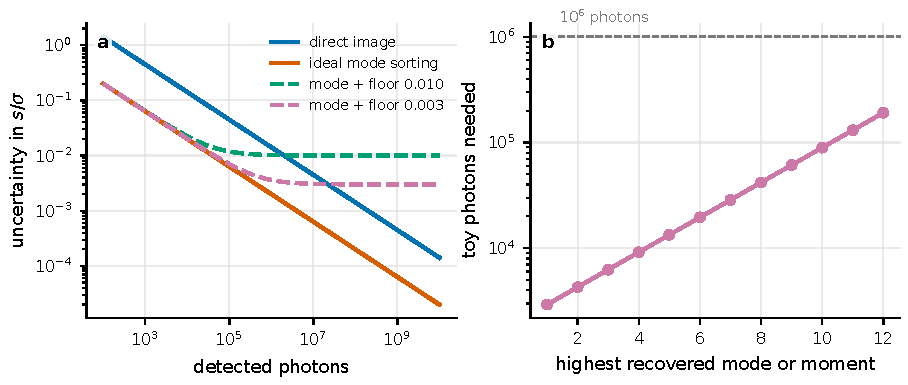
\includegraphics[width=0.96\linewidth]{figures/generated/chapter_21/ch21_superresolution_budget.pdf}
\caption{量子超分辨的光子预算和系统误差地板。左图显示 \(s=0.2\sigma\) 时直接成像和理想模式排序的统计误差标度；模式排序显著降低误差，但 \(0.003\sigma\)--\(0.01\sigma\) 的模式/质心误差地板会终止继续改善。右图用 toy model 表示恢复更高阶矩或模式所需光子数快速上升，复杂图像不能从少数光子中任意恢复。}
\label{fig:ch21-superresolution}
\end{figure}

天文语境里还要区分源本身的相干性和传播后的一阶空间相干。部分相干源会改变模式概率，相关文献中对 Rayleigh curse 是否重新出现的讨论围绕这个条件展开 \citep{2017NJPh...19b3054T,2017PhRvA..95f3847A,2018Optic...5.1177P,2018Optic...5.1382L,2019Optic...6..400T}。因此，把“两点非相干高斯源”的结论直接推广到星系、吸积盘、喷流或强透镜弧会失去适用条件。给定源模型、PSF、背景和测量基后，模式测量可以提高某些参数的信息效率；离开这些条件，超分辨只是一个口号。

\section{天体 laser、maser 和非 Poisson 统计最容易混淆在哪里}

“天体 laser/maser 一定有 \(g^{(2)}=1\)”也是误区。受激辐射可以产生高亮温、窄线和强偏振，但天体环境通常没有实验室稳定谐振腔。未饱和 maser、饱和 maser、速度相干路径、泵浦涨落、多个斑点叠加和连续谱背景都会改写光子统计 \citep{1982RvMP...54.1225E,1992ARA&A..30...75E,1985ARA&A..23..169D}。Eta Carinae 的 Weigelt blobs 中，Fe II 和 O I 线的自然激光候选需要同时看 Ly\(\alpha\) 泵浦、能级反转、线宽、空间位置和连续谱扣除；Brown--Twiss--Townes heterodyne correlation 被提出用来测窄 Fe II 线宽 \citep{2004A&A...428..497J,2005MNRAS.364..731J,2005NewA...10..361J,2008AIPC..984..216D}。

若观测光由多个独立成分叠加，总强度 \(I=\sum_a I_a\)，且不同成分之间没有强度相关，则零延迟相关超额近似为
\begin{equation}
  g_{\rm mix}^{(2)}(0)-1
  =
  \sum_a f_a^2\left[g_a^{(2)}(0)-1\right],
  \qquad
  f_a=\frac{\langle I_a\rangle}{\sum_b\langle I_b\rangle}.
  \label{eq:ch21-mixture}
\end{equation}
\begin{formulaexplain}[公式 (21.2) 解读]
\(f_a\) 是第 \(a\) 个成分的通量分数。相关超额按 \(f_a^2\) 加权，所以少量热连续谱或多成分混合会把 \(g^{(2)}\) 解释变得很危险。
\end{formulaexplain}
\(f_a\) 是通量分数，无量纲。一个占总通量 \(20\%\) 的热成分，即使自身 \(g^{(2)}(0)-1=1\)，混合后也只贡献 \(0.04\) 的对比度；若再有 \(M=100\) 个模式和 \(\tau_c/\Delta t=10^{-5}\)，观测对比度变成 \(4\times10^{-9}\)。反过来，未饱和受激线若带有泵浦强度噪声，可能产生超 Poisson 统计；这种结果要先分离谱线、连续谱和仪器响应，不应直接归因于新物理。

\begin{figure}[tbp]
\centering
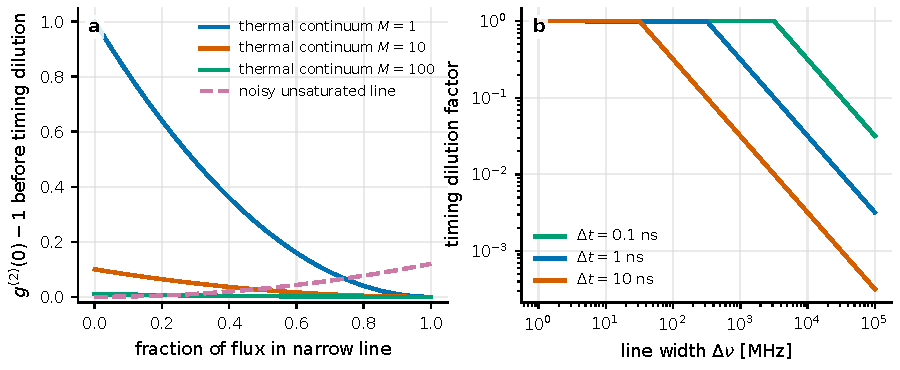
\includegraphics[width=0.96\linewidth]{figures/generated/chapter_21/ch21_maser_mixed_statistics.pdf}
\caption{天体 maser/laser 候选中的混合统计。左图显示窄线通量分数增加时，热连续谱聚束按通量分数平方被稀释；若窄线本身有未饱和强度噪声，则会出现另一条超 Poisson 分支。右图显示谱线宽度和电子学时间 bin 对相关对比度的稀释，MHz--GHz 线宽需要 ns 或更快的时间响应才能保留较大峰值。}
\label{fig:ch21-maser}
\end{figure}

非 Poisson 统计同样有普通来源。一个随机变源可以看成 Cox process：在给定瞬时率 \(\Lambda\) 时计数是 Poisson，但 \(\Lambda\) 本身随时间或环境变化。于是
\begin{equation}
  F_{\rm Fano}
  \equiv \frac{{\rm Var}(N)}{\mathbb E(N)}
  =
  1+\frac{{\rm Var}(\Lambda)}{\mathbb E(\Lambda)}
  \label{eq:ch21-fano}
\end{equation}
\begin{formulaexplain}[公式 (21.3) 解读]
\(F_{\rm Fano}\) 是方差与均值之比。若瞬时率 \(\Lambda\) 自身在变，计数会自然变成 super-Poisson，不必先诉诸非经典光源。
\end{formulaexplain}
在合适时间 bin 中大于 1。死时间会压低短间隔事件，使 \(F_{\rm Fano}<1\) 或在短延迟出现负相关；afterpulsing 会在探测器特征时间后产生正相关。第六章给出的 afterpulsing 概率 \(10^{-4}\)--\(10^{-2}\) 已足以污染许多短延迟搜索。判断“非 Poisson”之前，应先画 Fano factor 随 bin 宽变化、短延迟自相关和互相关、暗场数据、off-source 数据以及 time-shift 背景。

\begin{figure}[tbp]
\centering
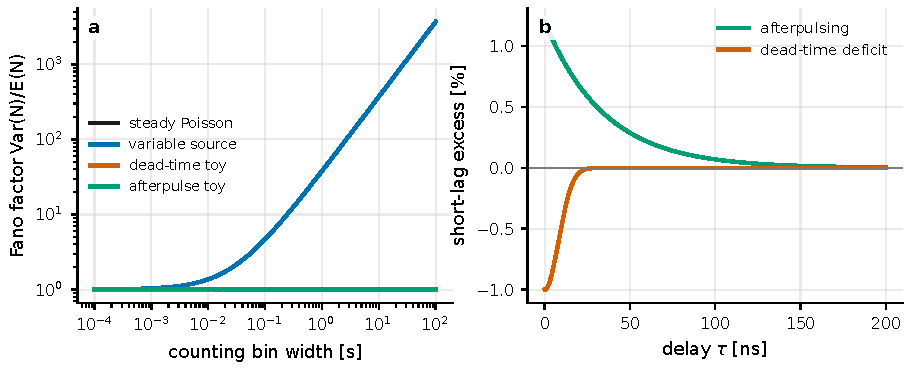
\includegraphics[width=0.96\linewidth]{figures/generated/chapter_21/ch21_nonpoisson_diagnostics.pdf}
\caption{非 Poisson 统计的普通来源。左图用 Fano factor 展示稳态 Poisson、慢变源、死时间和 afterpulsing 的不同标度；慢变源在长 bin 中变得 super-Poisson，死时间造成 under-dispersion。右图显示 afterpulsing 和死时间在短延迟相关函数中的相反形状，这些仪器特征应先从暗场和交叉通道中量化。}
\label{fig:ch21-nonpoisson}
\end{figure}

\section{假警报怎样画出新物理边界}

单次小概率事件也常被误读为发现。若一次检验的尾概率是 \(p_0\)，独立试验数为 \(N_{\rm trial}\)，至少出现一次的概率是
\begin{equation}
  p_{\rm any}=1-(1-p_0)^{N_{\rm trial}}
  \simeq N_{\rm trial}p_0
  \quad (N_{\rm trial}p_0\ll1).
  \label{eq:ch21-trials}
\end{equation}
\begin{formulaexplain}[公式 (21.4) 解读]
\(p_0\) 是单次检验的尾概率，\(N_{\rm trial}\) 是试验次数。搜索空间越大，至少看到一次偶然峰的概率越高，因此要报告全局显著性。
\end{formulaexplain}
\(N_{\rm trial}\) 可以来自时间 bin 数、频率通道数、基线数、目标数、模型网格和事后挑选的窗口。若每晚搜索 \(10^6\) 个候选延迟/频率/目标组合，单次 \(p_0=10^{-5}\) 的事件几乎必然会出现。多重检验不是形式主义；它决定一个峰是天文信号、仪器异常还是搜索空间中的自然尾部。

\begin{figure}[tbp]
\centering
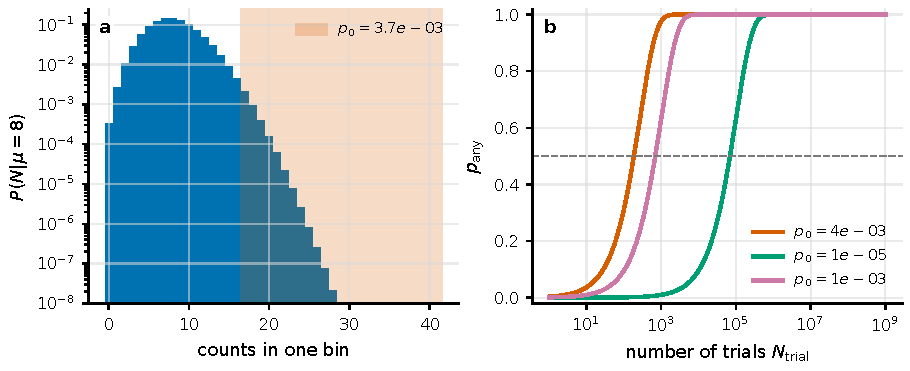
\includegraphics[width=0.96\linewidth]{figures/generated/chapter_21/ch21_poisson_false_alarm.pdf}
\caption{Poisson 尾部和多重检验。左图中 \(\mu=8\) 的单个 bin 偶尔会出现 \(N\ge17\) 的高计数尾部；右图显示同样的单次 \(p_0\) 在大量 trial 中如何变成很高的全局假警报概率。事件表搜索、周期搜索、跨频相关和暂现源筛选都要报告 \(N_{\rm trial}\) 或等效全局显著性。}
\label{fig:ch21-false-alarm}
\end{figure}

“量子天文学”也不等于“量子引力”。前面大部分内容研究的是光场统计、模式测量、相干函数、仪器和信息极限。黑洞、CMB、轴子、宇宙双折射或暗物质透镜可以进入这条主线，是因为它们能写成可观测的时间、频率、偏振或空间相关量，并非因为每个话题都需要 Planck 尺度物理。一个可检查的异常信号需要把数据来源拆开：
\begin{equation}
  d_{\rm obs}=d_{\rm sky}(\boldsymbol\theta)
  +d_{\rm inst}(\boldsymbol\phi)
  +d_{\rm sel}(\boldsymbol\psi)
  +n,
  \label{eq:ch21-data-model}
\end{equation}
\begin{formulaexplain}[公式 (21.5) 解读]
\(d_{\rm obs}\) 是观测数据，右边把天空、仪器、选择函数和噪声分开。任何“新物理”解释都应先证明普通天体项和仪器项不能解释数据。
\end{formulaexplain}
其中 \(d_{\rm obs}\) 是数据向量，例如延迟直方图、\(|V|^2\)、偏振相关或事件时间；\(d_{\rm sky}\) 是天体模型；\(d_{\rm inst}\) 是仪器模型；\(d_{\rm sel}\) 是选择函数；\(n\) 是噪声。若这四项还没有分开，异常峰、偏振旋转或非 Poisson 计数都不应直接归因于新物理。

研究计划的最后一页应回到新增观测量：它是平均强度、二阶相关、跨频协方差、偏振相关，还是模式计数。若目标是二阶相关，就列出事件表怎样生成延迟直方图、time-shift 背景怎样定义、零延迟峰怎样标定；若目标是偏振或模式计数，就列出通道定义、响应矩阵、背景项和协方差。每个量都要配上单位、典型范围和适用条件，例如热光、高斯 PSF、弱光、少参数源模型或稳定仪器响应。null test 至少应从 time-shift、off-source、off-band、暗场、错偏振和注入恢复中选出两个；全局显著性和系统误差地板要同时进入结论。


\chapter{从白皮书到研究计划}
\label{chap:22}

\begin{chapteropening}
量子天文学的研究计划要能执行，也要能失败。路线图需要写清观测量、数据产品、误差预算、里程碑和风险登记；读者应能把这一章直接改写成 proposal 的工作包、验收指标和失败判据。现代强度干涉白皮书、Cherenkov 阵列结果、谱复用方案、Type Ia 距离模型、量子网络望远镜设想和开放数据工具，把可做的近期工作和还需要 pathfinder 的远期工作分开 \citep{1956Natur.178.1046H,1974iiia.book.....H,2003RPPh...66..789M,2018SPIE10548E..1KO,2026arXiv260212717K,2017ICRC...35..828K,2019ICRC...36..714K,2020NatAs...4.1164A,2024MNRAS.529.4387A,2025PhRvD.111h3047K,2023PhRvL.130p0801M,2026PhRvA.113a2608P}。
\end{chapteropening}

\section{2026 到 2030：怎样把强度干涉做成常规数据产品}

近期目标是把已经可行的强度干涉变成可重复的数据产品，量子网络望远镜仍属于后续阶段。这个阶段的主要观测量是 \(\hat g^{(2)}_{ab}(\tau)\)、\(|V_{ab}|^2\)、目标光子率、零基线对比度、背景稀释因子和每条基线的协方差。VERITAS 和 MAGIC 已经证明 IACT 阵列可以做亮星强度干涉，\(\beta\) UMa 和 \(\gamma\) Cas 的结果显示，恒星角直径、快速自转和非球对称模型已经进入真实科学阶段 \citep{2020NatAs...4.1164A,2024MNRAS.529.4387A,2024ApJ...966...28A,2025ApJ...995..191A}。小口径 Sirius 演示和 AQuEye/IquEye 方案说明，教学实验、路径验证和大设施观测可以共用同一套事件表和相关器语言 \citep{2016SPIE.9907E..0NZ,2025MNRAS.537.2527M}。

近期项目的成熟度要写成可验收指标，不能停在“探测器可用”或“望远镜足够大”：
\begin{equation}
  \bm{r}=
  \left(
  \frac{R_\gamma}{R_{\rm req}},
  \frac{\sigma_{t,{\rm req}}}{\sigma_t},
  \frac{\beta_0}{\beta_{\rm req}},
  \frac{\sigma_{{\rm sys,req}}}{\sigma_{\rm sys}},
  \frac{N_{\rm cal}}{N_{{\rm cal,req}}}
  \right).
  \label{eq:ch22-readiness-vector}
\end{equation}
\begin{formulaexplain}[公式 (22.1) 解读]
\(\bm r\) 是项目成熟度向量，每一项都是实际能力与需求的比值。只有光子率、计时、对比度、系统误差和校准样本同时达标，近期项目才算闭合。
\end{formulaexplain}
\(R_\gamma\) 是每台望远镜的有效光子率，单位 \({\rm s}^{-1}\)；\(\sigma_t\) 是相对时间同步误差，单位 ps 或 ns；\(\beta_0\) 是零基线相关对比度，无量纲；\(\sigma_{\rm sys}\) 是校准后的系统误差地板；\(N_{\rm cal}\) 是可用校准星或校准观测数。若 \(R_\gamma/R_{\rm req}>1\) 但 \(\sigma_{\rm sys}\) 比目标 \(|V|^2\) 信号还大，项目仍然不成熟。强度干涉阵列研究反复强调，基线长度、\(u,v\) 覆盖、背景控制和零基线校准要一起闭合 \citep{2006ApJ...649..399L,2013APh....43..331D,2022MNRAS.512.1722K}。

\begin{figure}[tbp]
\centering
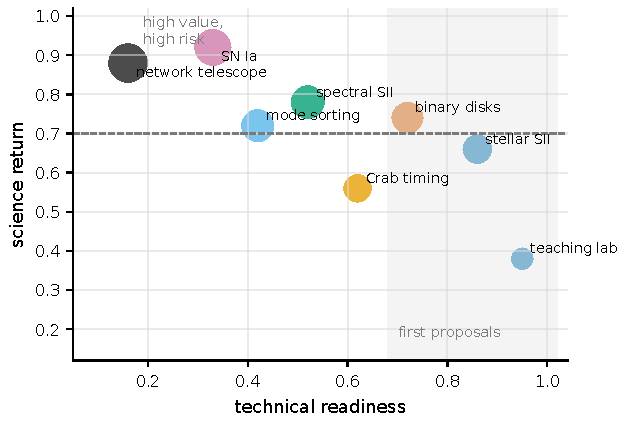
\includegraphics[width=0.86\linewidth]{figures/generated/chapter_22/ch22_roadmap_trade_space.pdf}
\caption{路线图中的技术成熟度、科学回报、成本和风险。右上方但成熟度较高的任务适合写成近期 proposal；左上方的任务有高科学价值但需要先做路径验证。点大小表示成本压力，位置表示技术成熟度和科学回报的相对判断。}
\label{fig:ch22-trade-space}
\end{figure}

2026--2030 年的第一批论文应尽量具体。可执行题目可以写成“用四台 IACT 在 416 nm 附近测量 10--30 颗亮星角直径，并给出公开相关器和校准库”；也可以写成“用同一套 pipeline 比较双星、Be 星盘和快速自转星的 \(|V|^2\) 模型”。每篇论文都应发布事件表格式说明、相关器版本、time-shift null test、校准星表、基线几何和后验样本。这样即使部分目标没有检出，也能留下可复用的仪器知识。

\section{2030 到 2040：多通道事件表要多出什么}

中期目标是把“一个蓝光滤光片上的 \(|V|^2\)”扩展成多通道事件表。光谱分辨强度干涉可以比较谱线内外的角尺度；偏振分辨相关可以检查磁场几何、散射和强场辐射；皮秒级事件表可以把光子统计作为新的时域数据产品。谱复用的吸引力在于，每个光谱通道的相干时间变长，而多个通道又可以并行累加 SNR；但代价是数据率、通道间校准和色散模型变复杂 \citep{2021sf2a.conf..335L,2022MNRAS.512.1722K,2024MNRAS.529.4387A}。

多通道阶段的基本数据产品可以写成
\begin{equation}
  \bm{d}=
  \left\{
  H_{ab}^{\nu p}(\tau),
  \widehat{|V_{ab}^{\nu p}|^2},
  C_{\nu_i\nu_j}^{p_i p_j},
  \bm{\Sigma}
  \right\}.
  \label{eq:ch22-data-vector}
\end{equation}
\begin{formulaexplain}[公式 (22.2) 解读]
\(\bm d\) 是多通道阶段的数据产品集合。它不只包含 \(|V|^2\)，还包括延迟直方图、跨频/跨偏振协方差和完整协方差矩阵。
\end{formulaexplain}
\(H_{ab}^{\nu p}\) 是望远镜 \(a,b\)、频率通道 \(\nu\)、偏振通道 \(p\) 的延迟直方图；\(|V|^2\) 是校准后的空间相干观测量；\(C_{\nu_i\nu_j}^{p_i p_j}\) 是跨频或跨偏振协方差；\(\bm{\Sigma}\) 是这些数据之间的协方差矩阵。只写“多通道量子观测”还不够；这些量怎样存储、归一化和发布，决定项目是否已经到工程阶段。

\begin{figure}[tbp]
\centering
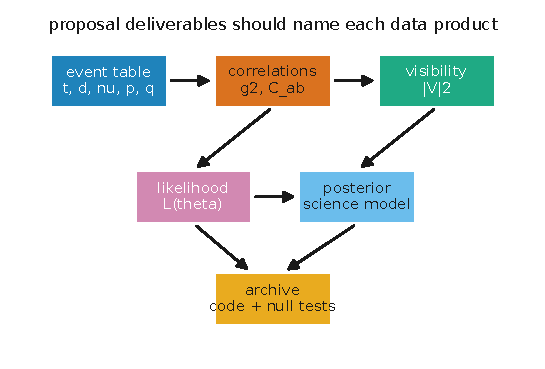
\includegraphics[width=0.88\linewidth]{figures/generated/chapter_22/ch22_data_product_stack.pdf}
\caption{从 proposal 到公开数据的产品链。事件表保留到达时间、望远镜、频率、偏振和质量标记；相关器把它变成 \(g^{(2)}\) 和协方差；空间模型给出 \(|V|^2\)；似然和后验连接到天体参数；归档要包含代码、版本和 null test。}
\label{fig:ch22-data-products}
\end{figure}

Type Ia 超新星距离是中期科学案例的典型高风险高回报项目。它需要快速触发、km 级到十 km 级基线、爆炸时间、速度模型、光球非球对称和强度干涉角半径联合建模。Kim、Nugent、Chen 和合作者的 toy model 给出了可行性边界：近邻、明亮、早期发现的事件才值得进入干涉跟进 \citep{2025PhRvD.111h3047K}。自然激光、Crab pulsar 光子统计、Be 星盘谱线和 AGN BLR 几何也可写成同一类计划，但每一个都要先说明触发率、可观测窗口、背景和失败判据。

\section{2040 以后：量子网络望远镜何时才是主线}

远期目标要分层写。本地模式排序和相位敏感测量不需要完整量子网络，也能提高小分离和亮度矩估计的信息效率 \citep{2016PhRvX...6c1033T,2017PhRvL.118g0801T}。two-photon astrometry、单光子辅助或线性光学 pathfinder 的目标，是把天文光和实验室量子资源稳定耦合 \citep{2023PhRvL.130p0801M,2024SPIE13095E..1NR}。纠缠辅助长基线干涉需要纠缠分发率、量子存储时间、频率转换效率、Bell fidelity 和天文同步共同达标，属于更后面的阶段 \citep{2025PhRvA.111d3701M,2025PhRvR...7d3278Z,2026PhRvA.113a2608P,2026Natur.651..326S}。

量子网络望远镜的资源门槛已经在第 \ref{chap:17} 章式 \eqref{eq:ch17-entanglement-rate}、\eqref{eq:ch17-memory-time} 和 \eqref{eq:ch17-effective-fidelity} 中写成链路率、存储时间和有效保真度的约束。proposal 要把同一组量放进验收表：\(R_{\rm ent}\) 是纠缠对产生率，单位 \({\rm s}^{-1}\)；\(\eta_{\rm link}\)、\(\eta_{\rm mem}\)、\(\eta_{\rm conv}\) 分别是链路、存储和频率转换效率；\(R_{\gamma,{\rm useful}}\) 是实际进入目标模式和时间窗的天文光子率；\(T_{\rm mem}\) 是可用存储时间；\(B/c\) 是基线光行时。\(B=1000\,{\rm km}\) 时 \(B/c\simeq3.3\,{\rm ms}\)，地面 km 级基线只需 \(\mu{\rm s}\) 到 ms 级同步，但全球或空间基线会把存储和分发压力迅速放大。链路损耗、存储退相干和有用光子率任何一项不达标，网络方案都还不足以替代常规强度干涉或振幅干涉。

\begin{figure}[tbp]
\centering
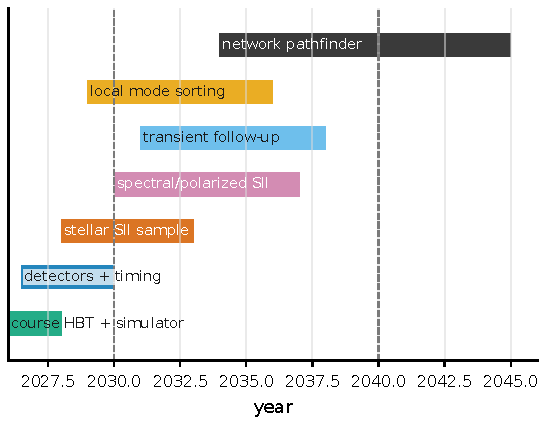
\includegraphics[width=0.92\linewidth]{figures/generated/chapter_22/ch22_program_timeline.pdf}
\caption{从课程 HBT 到量子网络 pathfinder 的阶段性时间线。绿色和蓝色任务建立人才、事件表、计时和校准；橙色和紫色任务产出第一代科学样本和多通道相关；黑色远期任务只有在本地模式排序、链路和存储指标达标后才应写成设施路线。}
\label{fig:ch22-timeline}
\end{figure}

\section{研究计划怎样写}

\Needspace{11\baselineskip}
一个可执行里程碑要把观测量和验收标准同时写清：
\begin{equation}
  m_j=
  \left(
  O_j,\,
  \sigma_{O,j}^{\rm goal},\,
  T_j,\,
  N_{{\rm null},j},\,
  D_{{\rm release},j}
  \right).
  \label{eq:ch22-milestone}
\end{equation}
\begin{formulaexplain}[公式 (22.3) 解读]
\(m_j\) 是第 \(j\) 个里程碑。它同时指定观测量、目标精度、时间、null test 数和发布数据，避免路线图只停在愿景。
\end{formulaexplain}
\(O_j\) 是观测量，例如 \(g^{(2)}(0)-1\)、\(|V|^2\)、谱线内外角尺度比或 \(D_A\)；\(\sigma_O^{\rm goal}\) 是目标精度；\(T_j\) 是完成日期或所需观测时间；\(N_{\rm null}\) 是要通过的 null test 数；\(D_{\rm release}\) 是要发布的数据产品。近期项目可以要求 \(N_{\rm null}\ge2\)：time-shift 和 off-source；中期多通道项目应要求 \(N_{\rm null}\ge4\)：time-shift、off-band、错偏振和注入恢复；远期网络项目还应包含链路保真度和存储退相干的独立验收。

\begin{figure}[tbp]
\centering
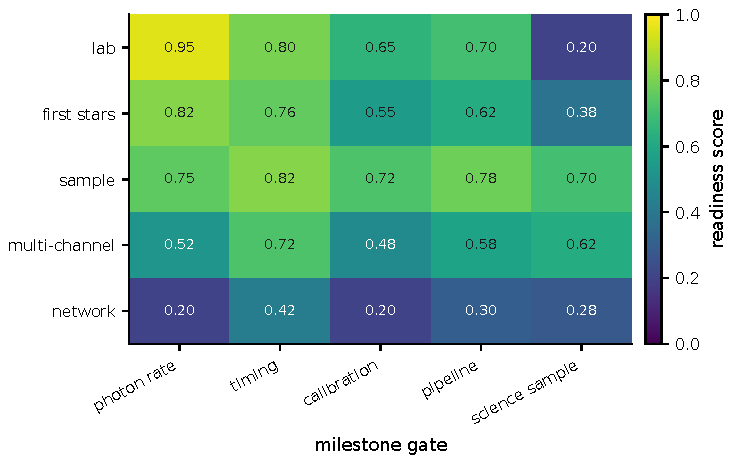
\includegraphics[width=0.92\linewidth]{figures/generated/chapter_22/ch22_milestone_gates.pdf}
\caption{不同阶段的里程碑门槛矩阵。课程实验和第一代恒星 SII 在光子率、计时和 pipeline 上已经较成熟，但多通道校准和网络阶段仍有明显缺口。数字只是 proposal 中应显式量化的 readiness score 示例，并不代表设施承诺。}
\label{fig:ch22-gates}
\end{figure}

误差预算要从第一版 proposal 就写清楚，并沿用第 \ref{chap:18} 章式 \eqref{eq:ch18-error-budget} 的分解。\(\sigma_{\rm stat}\) 来自 Poisson 或相关计数噪声；\(\sigma_{\rm cal}\) 来自零基线对比度、时间同步、偏振和光谱响应；\(\sigma_{\rm bg}\) 来自夜天光、连续谱或伴星背景；\(\sigma_{\rm model}\) 来自恒星盘、超新星光球、BLR 或 maser 几何；\(\sigma_{\rm sel}\) 来自触发、天气和目标选择。统计采样可以用 MCMC、nested sampling 或后验预测检查实现，但这些工具无法替代物理误差项本身 \citep{2013PASP..125..306F,2009MNRAS.398.1601F,1979ApJ...228..939C,2013ApJ...764..167S,2025ApJ...988...23P}。

\begin{figure}[tbp]
\centering
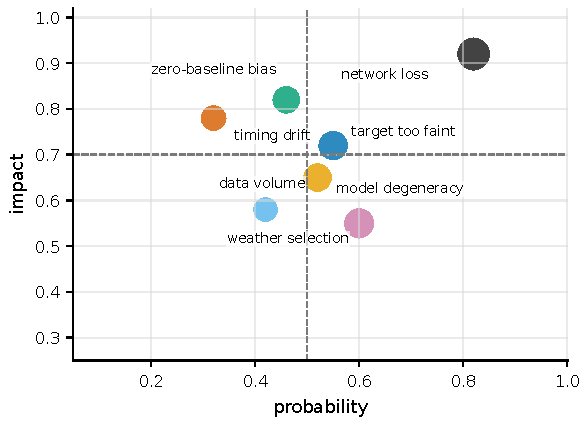
\includegraphics[width=0.86\linewidth]{figures/generated/chapter_22/ch22_risk_register.pdf}
\caption{路线图的风险登记图。右上角的风险需要在项目开始前配套缓解方案：例如网络损耗需要先做短基线 pathfinder，零基线偏差需要校准星库，目标过暗需要明确的触发和放弃标准。点越大表示缓解方案越弱。}
\label{fig:ch22-risk}
\end{figure}

风险登记表要和失败判据一起写。若目标星等比预期暗 1 mag，光子率下降到约 40\%；若系统误差地板停在 \(3\times10^{-5}\)，许多 \(|V|^2\) 小信号不再可测；若 Type Ia 触发晚 10 天，角半径更大但光度下降、模型不确定性上升；若网络链路每天只给很少高保真 entangled pairs，科学模式就应退回本地模式排序或强度干涉。路线图可以失败，但失败要告诉下一阶段该改什么。

\section{从课程项目怎样长成研究课题}

课程项目可以从第 \ref{chap:20} 章开始：桌面 HBT、事件表模拟、均匀圆盘拟合、SPADE Fisher 信息和假警报计算。较小的研究题目适合围绕一个 pipeline 展开，例如时间同步、相关器、校准库、目标样本或 open-data notebook。更完整的科学题目可以瞄准 Be 星 H\(\alpha\) 盘的谱线角尺度、快速自转星多基线模型、Crab pulsar 相位分辨光子统计、Type Ia 距离 toy model 的系统误差，或者本地模式排序和自适应光学的联合实验。大型合作项目再把这些课题接到 CTAO/IACT、ELT/VLTI/CHARA、Rubin、SKA、LIGO/Virgo/KAGRA/ET 或量子网络实验室。

一个项目至少要列出新增观测量、事件表字段、数据估计步骤、符号单位、典型范围、两个以上 null test，以及失败后仍能留下的数据、代码或仪器约束。这样的计划可以被复现、审查和改进；否则“量子”只停留在题目上。


\appendix
\chapter{常用公式索引}
\label{app:a}

公式索引列出每个关系第一次稳定出现的位置。后续章节需要同一组量时，优先回到这里和正文对应处查符号、单位、数量级和适用条件。

\section{事件表、计数和似然}
\label{appsec:a-observables}

\begin{longtable}{p{0.22\linewidth}p{0.31\linewidth}p{0.37\linewidth}}
\toprule
主题 & 位置 & 使用时检查 \\
\midrule
光子事件表字段 & 第 \ref{chap:e00} 章；仪器层扩展见第 \ref{chap:e13} 章 & 时间基准、探测器或望远镜编号、频率通道、偏振、质量标记、空间像素和权重。 \\
时间标定 & 第 \ref{chap:e13} 章 & 原始 TDC 时间、时钟漂移、光路延迟、barycentric 校正和绝对同步。 \\
Poisson 计数 & 第 \ref{chap:e00} 章 & 期望计数是否包含源变化、背景、曝光、选择函数和死时间。 \\
未分箱点过程似然 & 第 \ref{chap:e14} 章 & 事件时间是否保留；rate model 是否随时间、能量或质量窗口变化。 \\
分箱 Poisson 似然 & 第 \ref{chap:e14} 章；教学投影见第 \ref{chap:e26} 章 & bin 宽是否比物理时间尺度、仪器响应和统计计数要求都合适。 \\
延迟和 pair count & 第 \ref{chap:e14} 章 & 延迟窗口、time-shift 背景、随机符合、重复事件和质量筛选。 \\
\(g^{(2)}\) 估计量 & 第 \ref{chap:e14} 章 & 归一化、背景窗口、零延迟峰宽和不相关通道检查。 \\
协方差和后验 & 第 \ref{chap:e14} 章 & 数据点之间是否相关；先验和似然是否写在同一个数据向量上。 \\
\bottomrule
\end{longtable}

\section{相干、可见度和强度干涉}
\label{appsec:a-coherence}

\begin{longtable}{p{0.22\linewidth}p{0.31\linewidth}p{0.37\linewidth}}
\toprule
主题 & 位置 & 使用时检查 \\
\midrule
复可见度 & 第 \ref{chap:e10} 章 & 角坐标单位、投影基线、波长、窄视场近似、带宽平均和源模型。 \\
均匀圆盘 & 第 \ref{chap:e10} 章 & 角直径是半径还是直径；是否需要边缘昏暗；基线是否覆盖第一零点附近。 \\
Siegert 关系 & 第 \ref{chap:e08} 章；空间 HBT 见第 \ref{chap:e10} 章 & 热光、混沌光或高斯场近似是否成立；偏振、频谱和模式数是否改变对比度。 \\
强度干涉观测模型 & 第 \ref{chap:e10} 章；校准模型见第 \ref{chap:e27} 章 & 零基线对比度、峰形、仪器串扰、选择函数和统计噪声是否分开。 \\
相干时间 & 第 \ref{chap:e08} 章；仪器通道形式见第 \ref{chap:e13} 章 & 滤光片带宽、谱线宽度、中心波长和频率单位。 \\
对比度稀释 & 第 \ref{chap:e08} 章 & 电子学响应、相关 bin、有效模式数、偏振平均和光谱平均。 \\
背景稀释 & 第 \ref{chap:e13} 章 & 目标通量分数、夜天光、伴星、谱线连续谱、暗计数和校准星。 \\
强度干涉 SNR & 第 \ref{chap:e10} 章；观测可行性见第 \ref{chap:e15} 章 & 光子率、望远镜面积、积分时间、等效带宽、\(|V|^2\) 和系统误差地板。 \\
基线数 & 第 \ref{chap:e10} 章 & 望远镜数增加会二次增加相关任务；数据率和校准复杂度同步上升。 \\
\bottomrule
\end{longtable}

\section{仪器响应和数据率}
\label{appsec:a-instrument}

\begin{longtable}{p{0.22\linewidth}p{0.31\linewidth}p{0.37\linewidth}}
\toprule
主题 & 位置 & 使用时检查 \\
\midrule
数据率 & 第 \ref{chap:e13} 章 & 采样时间、bit 数、光谱通道数、望远镜数和实时相关器能力。 \\
响应卷积 & 第 \ref{chap:e13} 章 & 探测器脉冲、线缆、放大器、digitizer 和软件相关窗口共同形成的响应核。 \\
jitter budget & 第 \ref{chap:e13} 章 & 探测器 jitter、时钟同步、光纤延迟、触发抖动和 barycentric 校正。 \\
事件表质量筛选 & 第 \ref{chap:e14} 章和第 \ref{chap:e26} 章 & 云层、饱和、死时间附近事件、异常背景、坏通道和目标高度。 \\
校准项分解 & 第 \ref{chap:e27} 章 & 天体项、仪器项、选择函数项和随机误差不能混在一个自由常数里。 \\
\bottomrule
\end{longtable}

\section{估计理论和模式测量}
\label{appsec:a-estimation}

\begin{longtable}{p{0.22\linewidth}p{0.31\linewidth}p{0.37\linewidth}}
\toprule
主题 & 位置 & 使用时检查 \\
\midrule
Fisher 信息 & 第 \ref{chap:e14} 章；空间模式例子见第 \ref{chap:e12} 章 & 参数、数据向量、协方差、导数和先验是否匹配实际观测。 \\
Cramér--Rao 下界 & 第 \ref{chap:e12} 章 & 下界是局部、无偏或渐近条件下的结果；系统误差不自动包含在内。 \\
高斯源量子 Fisher 信息 & 第 \ref{chap:e12} 章 & 源是否为弱、等亮、非相干双点源；PSF 是否已知。 \\
SPADE 模式概率 & 第 \ref{chap:e12} 章 & 模式基、中心定位、串扰矩阵、背景和有限光子数。 \\
SII Fisher 矩阵 & 第 \ref{chap:e12} 章 & \(|V|^2\) 误差、基线覆盖、参数退化和模型假设。 \\
混合统计 & 第 \ref{chap:e27} 章 & 多个独立成分的通量分数按平方稀释相关超额。 \\
Fano factor & 第 \ref{chap:e27} 章 & 慢变源、死时间和 afterpulsing 都能造成非 Poisson 计数。 \\
多重检验 & 第 \ref{chap:e27} 章 & 时间 bin、频率通道、基线、目标数和事后窗口都进入 trial 数。 \\
\bottomrule
\end{longtable}

\section{天体源模型}
\label{appsec:a-sources}

\begin{longtable}{p{0.22\linewidth}p{0.31\linewidth}p{0.37\linewidth}}
\toprule
主题 & 位置 & 使用时检查 \\
\midrule
亮温 & 第 \ref{chap:e16} 章 & 是否处在 Rayleigh--Jeans 近似；角尺度、距离和通量密度是否独立约束。 \\
热辐射和占有数 & 第 \ref{chap:e16} 章 & 频率、温度和模式占有数决定热光统计是否明显。 \\
同步辐射和偏振 & 第 \ref{chap:e16} 章 & 电子能谱、磁场、视角和 Faraday 效应。 \\
Maser 增益 & 第 \ref{chap:e16} 章 & 反转粒子数、速度相干长度、饱和程度和泵浦涨落。 \\
恒星有效温度 & 第 \ref{chap:e17} 章；案例版见第 \ref{chap:e25} 章 & 角直径、bolometric flux、消光和标定星。 \\
双星可见度 & 第 \ref{chap:e17} 章；科学案例见第 \ref{chap:e25} 章 & 通量比、角分离、位置角、多历元轨道和镜像退化。 \\
谱线/连续谱分离 & 第 \ref{chap:e17} 章；案例版见第 \ref{chap:e25} 章 & 谱线通量分数、连续谱角尺度和滤光片泄漏。 \\
瞬变角膨胀 & 第 \ref{chap:e20} 章；案例版见第 \ref{chap:e25} 章 & 触发时间、速度模型、非球对称和历元间演化。 \\
Type Ia 距离 toy model & 第 \ref{chap:e26} 章 & 光球速度、爆炸时间、角半径误差和辐射转移模型。 \\
\bottomrule
\end{longtable}

\section{传播、宇宙学和量子网络}
\label{appsec:a-propagation-network}

\begin{longtable}{p{0.22\linewidth}p{0.31\linewidth}p{0.37\linewidth}}
\toprule
主题 & 位置 & 使用时检查 \\
\midrule
色散延迟 & 第 \ref{chap:e21} 章 & 频率单位、DM 分解、通道内展宽和等离子体近似。 \\
Faraday 旋转 & 第 \ref{chap:e21} 章 & 偏振角约定、频率覆盖、内禀角和前景扣除。 \\
散射卷积 & 第 \ref{chap:e21} 章 & 多径传播、脉冲展宽、去卷积和选择效应。 \\
引力透镜 & 第 \ref{chap:e21} 章 & 质量模型、源位置、时间延迟和 microlensing。 \\
轴子偏振旋转 & 第 \ref{chap:e22} 章 & 频率依赖、时间调制、偏振标定和普通 Faraday 项。 \\
CMB 似然 & 第 \ref{chap:e23} 章 & \(C_\ell\)、协方差、前景和 cosmic variance。 \\
量子网络资源 & 第 \ref{chap:e24} 章 & 链路损耗、存储时间、频率转换、保真度和实际可用的天文光子率。 \\
观测误差预算 & 第 \ref{chap:e15} 章 & 统计、校准、背景、模型和选择函数误差是否都进入。 \\
proposal 里程碑 & 第 \ref{chap:e28} 章 & 可验收观测量、目标精度、null test、交付数据和失败判据。 \\
\bottomrule
\end{longtable}

\chapter{常用单位和数值}
\label{app:b}

这些表格集中列出写作、估算和审稿时最常用的单位与数量级。具体公式回到正文首次定义处；估算时同时检查单位、数量级和适用条件。

\section{基本常数和天文换算}
\label{appsec:b-constants}

\begin{longtable}{p{0.22\linewidth}p{0.30\linewidth}p{0.38\linewidth}}
\toprule
量 & 常用数值 & 使用提醒 \\
\midrule
光速 & \(c=2.998\times10^{10}\,{\rm cm\,s^{-1}}\) & 基线光行时 \(B/c\)：\(1\,{\rm km}\) 约 \(3.3\,\mu{\rm s}\)，\(1000\,{\rm km}\) 约 \(3.3\,{\rm ms}\)。 \\
Planck 常数 & \(h=6.626\times10^{-27}\,{\rm erg\,s}\) & 单个光子能量 \(E=h\nu=hc/\lambda\)。 \\
Boltzmann 常数 & \(k_{\rm B}=1.381\times10^{-16}\,{\rm erg\,K^{-1}}\) & 亮温、Planck 占有数和热噪声都需要它。 \\
Jansky & \(1\,{\rm Jy}=10^{-23}\,{\rm erg\,s^{-1}\,cm^{-2}\,Hz^{-1}}\) & AB 星等和光子率估算常从 Jy 开始。 \\
parsec & \(1\,{\rm pc}=3.086\times10^{18}\,{\rm cm}\) & \(1\,{\rm AU}\) 在 \(1\,{\rm pc}\) 处张角为 \(1''\)。 \\
太阳半径 & \(R_\odot=6.96\times10^{10}\,{\rm cm}\) & 估算恒星角直径和双星尺度时很常用。 \\
太阳光度 & \(L_\odot=3.83\times10^{33}\,{\rm erg\,s^{-1}}\) & 和 \(F_{\rm bol}\)、\(T_{\rm eff}\)、\(\theta\) 联用。 \\
\bottomrule
\end{longtable}

\section{角度、波长和基线}
\label{appsec:b-angle}

\begin{longtable}{p{0.22\linewidth}p{0.30\linewidth}p{0.38\linewidth}}
\toprule
量 & 常用数值 & 相关正文位置 \\
\midrule
角度换算 & \(1\,{\rm rad}=206265''\)；\(1\,{\rm mas}=4.848\times10^{-9}\,{\rm rad}\)；\(1\,\mu{\rm as}=4.848\times10^{-12}\,{\rm rad}\) & 第 \ref{chap:e00} 章、第 \ref{chap:e10} 章。 \\
可见光波长 & 蓝光强度干涉常在 \(400\)--\(450\,{\rm nm}\)；宽波段成像常用 \(500\)--\(800\,{\rm nm}\) & 第 \ref{chap:e10} 章、第 \ref{chap:e15} 章。 \\
衍射量级 & \(\lambda/B\) 在 \(500\,{\rm nm}\)、\(100\,{\rm m}\) 时约 \(1\,{\rm mas}\) & 百米级阵列适合亮星角直径。 \\
第一零点量级 & \(1\,{\rm mas}\) 均匀圆盘在 \(416\,{\rm nm}\) 附近第一零点约 \(100\,{\rm m}\) & 第 \ref{chap:e10} 章。 \\
\(\mu{\rm as}\) 结构 & \(10\,\mu{\rm as}\) 在 \(500\,{\rm nm}\) 下对应 \(\lambda/\theta\sim10\,{\rm km}\) & 近邻超新星、AGN 小尺度结构和远期长基线案例。 \\
投影基线 & \(B_\perp\) 随目标高度、时角和阵列几何变化 & 不能用固定物理基线替代整夜 \(u,v\) 覆盖。 \\
\bottomrule
\end{longtable}

\section{时间、频率和相干}
\label{appsec:b-time}

\begin{longtable}{p{0.22\linewidth}p{0.30\linewidth}p{0.38\linewidth}}
\toprule
量 & 常用数值 & 相关正文位置 \\
\midrule
频率换算 & \(500\,{\rm nm}\) 对应 \(6.0\times10^{14}\,{\rm Hz}\) & 光学带宽常需要在 \(\Delta\lambda\) 和 \(\Delta\nu\) 间换算。 \\
光学相干时间 & \(10\,{\rm nm}\) 级滤光片在可见光下通常给 \(10^{-14}\)--\(10^{-13}\,{\rm s}\) & 第 \ref{chap:e08} 章。 \\
相关 bin & 桌面实验可取 ps--ns；天文强度干涉常受电子学响应和数据率限制 & 第 \ref{chap:e14} 章、第 \ref{chap:e26} 章。 \\
探测器 jitter & 优秀 SPAD、PMT、TDC 系统可到几十 ps--ns；系统同步要单独标定 & 第 \ref{chap:e13} 章。 \\
死时间 & SPAD 常在 ns--\(\mu{\rm s}\)；PMT 和电子链也有恢复时间 & 死时间会在短延迟处制造负相关。 \\
afterpulsing & 概率可到 \(10^{-4}\)--\(10^{-2}\) 量级 & 会在探测器特征延迟处制造正相关。 \\
积分时间标度 & 纯统计误差常按 \(T^{-1/2}\) 下降 & 一旦达到系统误差地板，继续积分不会自动改善。 \\
\bottomrule
\end{longtable}

\section{光子率、星等和背景}
\label{appsec:b-photon-rate}

\begin{longtable}{p{0.22\linewidth}p{0.30\linewidth}p{0.38\linewidth}}
\toprule
量 & 常用数值 & 相关正文位置 \\
\midrule
AB 星等通量 & AB 零点见第 \ref{chap:e15} 章；光子率估算见第 \ref{chap:e00} 章 & 写 proposal 时同时给出带宽、效率、面积和背景。 \\
星等变化 & 目标暗 \(1\,{\rm mag}\)，光子率约降到原来的 \(10^{-0.4}\simeq0.40\) & 第 \ref{chap:e15} 章、第 \ref{chap:e28} 章。 \\
望远镜面积 & \(D=12\,{\rm m}\) 的理想几何面积约 \(113\,{\rm m^2}\)，实际有效面积还要乘效率和遮挡 & Cherenkov 望远镜光学效率、滤光片和探测器 QE 都要进入。 \\
背景稀释 & 目标通量分数为 \(f\) 时，二阶相关超额近似按 \(f^2\) 被压低 & 第 \ref{chap:e13} 章。 \\
窄线观测 & 谱线越窄，相干时间越长，但总光子数和滤光片泄漏可能变差 & Be 星盘、maser/laser 和 BLR 案例都要报告线/连续谱分离。 \\
夜天光 & 随月相、天顶距、滤光片和场镜大小变化 & 不要把暗场背景当成所有目标位置都适用。 \\
\bottomrule
\end{longtable}

\section{仪器和数据量}
\label{appsec:b-instrument}

\begin{longtable}{p{0.22\linewidth}p{0.30\linewidth}p{0.38\linewidth}}
\toprule
量 & 常用数值 & 相关正文位置 \\
\midrule
单路采样数据率 & \(\Delta t=4\,{\rm ns}\)、\(16\) bit、单通道时约 \(4\,{\rm Gb\,s^{-1}}\) & 第 \ref{chap:e13} 章。 \\
多通道膨胀 & 64 个光谱通道会把同一例子推到约 \(256\,{\rm Gb\,s^{-1}}\) 每望远镜 & 需要实时相关、压缩或片上累加。 \\
基线数 & 4 台望远镜为 6 条基线；60 台为 1770 条基线 & 第 \ref{chap:e10} 章。 \\
校准星 & 应尽量接近目标天空位置、颜色和亮度，且角直径已知 & 第 \ref{chap:e15} 章。 \\
质量切片 & 按天空透明度、目标高度、背景率、死时间和通道状态切分 & 只报告墙钟时间不足以复现实验。 \\
系统地板 & \(10^{-5}\)--\(10^{-4}\) 级相关幅度地板已足以支配许多 SII 目标 & 第 \ref{chap:e27} 章。 \\
\bottomrule
\end{longtable}

\section{天体物理数量级}
\label{appsec:b-astro}

\begin{longtable}{p{0.22\linewidth}p{0.30\linewidth}p{0.38\linewidth}}
\toprule
量 & 常用数值 & 相关正文位置 \\
\midrule
亮星角直径 & 近邻亮星常在 \(0.2\)--\(5\,{\rm mas}\) 量级 & 第 \ref{chap:e17} 章、第 \ref{chap:e25} 章。 \\
Type Ia 早期速度 & 光球速度常为 \(8000\)--\(15000\,{\rm km\,s^{-1}}\) & 第 \ref{chap:e20} 章、第 \ref{chap:e26} 章。 \\
近邻超新星角半径 & \(20\,{\rm Mpc}\)、\(v=10^4\,{\rm km\,s^{-1}}\)、15 天时约数 \(\mu{\rm as}\) & km 到十 km 级基线才有明显信息。 \\
Crab 周期 & 约 \(33\,{\rm ms}\) & 相位分辨光子统计需要保留绝对时间。 \\
AGN 宽线区 & 光变延迟常为天到月，角尺度通常极小 & 需要把 reverberation、角位移和模型先验合并。 \\
CMB 温度 & \(2.725\,{\rm K}\) & 第 \ref{chap:e23} 章；光学光子统计不能直接套用。 \\
\bottomrule
\end{longtable}

\chapter{术语表}
\label{app:c}

常用术语按工作定义、容易混用的边界和主要阅读位置列出。定义只保留查阅时最需要的边界；完整物理图像、公式、数量级和文献见正文对应章节。

\section{数据、统计和推断}
\label{appsec:c-data}

\begin{longtable}{p{0.20\linewidth}p{0.45\linewidth}p{0.25\linewidth}}
\toprule
术语 & 本书用法 & 主要位置 \\
\midrule
事件表 & 逐光子记录，至少包含时间和探测通道；可扩展频率、偏振、位置、质量标记和权重。不要把它等同于已经分箱的光变曲线。 & 第 \ref{chap:e00}、\ref{chap:e13}、\ref{chap:e14} 章。 \\
光变曲线 & 事件表在时间轴上的投影，通常丢掉通道、偏振和单事件间隔信息。 & 第 \ref{chap:e00}、\ref{chap:e14} 章。 \\
曝光函数 & 描述有效观测时间、面积、效率和选择函数怎样随时间或通道变化的函数。 & 第 \ref{chap:e14}、\ref{chap:e15} 章。 \\
live time & 扣除死时间、坏天气、饱和和质量筛选后的有效积分时间。 & 第 \ref{chap:e13}、\ref{chap:e15} 章。 \\
Poisson 过程 & 给定瞬时率后，事件独立到达的计数模型；非稳态源要使用随时间变化的率。 & 第 \ref{chap:e00}、\ref{chap:e14}、\ref{chap:e27} 章。 \\
Cox process & 率本身随机变化的 Poisson 过程；可产生 super-Poisson 计数，不必是新物理。 & 第 \ref{chap:e27} 章。 \\
似然 & 在给定模型参数下得到观测数据的概率密度或概率质量。不要和后验混用。 & 第 \ref{chap:e14}、\ref{chap:e15} 章。 \\
后验 & 似然与先验结合后的参数分布。报告后验时要说明先验和数据向量。 & 第 \ref{chap:e14}、\ref{chap:e26} 章。 \\
Fisher 信息 & 似然对参数局部敏感度的度量；不是系统误差的自动替代品。 & 第 \ref{chap:e00}、\ref{chap:e14}、\ref{chap:e12} 章。 \\
协方差矩阵 & 数据点或参数误差之间相关性的矩阵。多基线 \(|V|^2\) 点通常不能默认独立。 & 第 \ref{chap:e14}、\ref{chap:e15} 章。 \\
Fano factor & 计数方差与均值的比值，用于诊断慢变源、死时间和 afterpulsing。 & 第 \ref{chap:e27} 章。 \\
trial factor & 多重检验造成的全局显著性修正。时间 bin、频率通道、基线和目标数都可能贡献 trial。 & 第 \ref{chap:e27} 章。 \\
null test & 应该消除天体信号而保留仪器或背景结构的检查，例如 time-shift、off-source、off-band、错偏振。 & 第 \ref{chap:e14}、\ref{chap:e26}、\ref{chap:e27} 章。 \\
\bottomrule
\end{longtable}

\section{量子光学和相干函数}
\label{appsec:c-optics}

\begin{longtable}{p{0.20\linewidth}p{0.45\linewidth}p{0.25\linewidth}}
\toprule
术语 & 本书用法 & 主要位置 \\
\midrule
模式 & 光场的一个可分辨自由度，可以是空间、时间、频率或偏振模式。模式数决定聚束对比度是否被稀释。 & 第 \ref{chap:e06}、\ref{chap:e08} 章。 \\
占有数 & 单个模式中的平均光子数；射电常大，光学天文单模式常很小。 & 第 \ref{chap:e06}、\ref{chap:e16} 章。 \\
相干态 & Poisson 光子数分布、\(g^{(2)}(0)=1\) 的理想光态；天体 laser/maser 不一定等同于稳定相干态。 & 第 \ref{chap:e06}、\ref{chap:e27} 章。 \\
热态 & 单模式下有聚束的混沌光场；多模式和有限响应会降低观测对比度。 & 第 \ref{chap:e06}、\ref{chap:e08} 章。 \\
压缩态 & 一个正交量噪声低于真空、另一个正交量升高的光场状态；宇宙学涨落中也出现相关语言。 & 第 \ref{chap:e06}、\ref{chap:e23} 章。 \\
密度矩阵 & 描述纯态或混合态的状态对象；当天体光源由许多不可分辨成分组成时特别自然。 & 第 \ref{chap:e06}、\ref{chap:e24} 章。 \\
退相干 & 相位关系因环境、平均或未观测自由度而不可用；不要简单等同于“没有量子”。 & 第 \ref{chap:e06}、\ref{chap:e23} 章。 \\
一阶相干函数 & 描述场振幅相关；振幅干涉和复可见度都依赖这个量。 & 第 \ref{chap:e08}、\ref{chap:e10} 章。 \\
二阶相干函数 & 描述强度或探测事件的相关；HBT 和光子统计的核心观测量。 & 第 \ref{chap:e08}、\ref{chap:e14} 章。 \\
聚束 & 热光或混沌光在零延迟附近的正二阶相关超额。 & 第 \ref{chap:e00}、\ref{chap:e08} 章。 \\
反聚束 & \(g^{(2)}(0)<1\) 的非经典光子统计特征；天文环境中极难保持。 & 第 \ref{chap:e08}、\ref{chap:e27} 章。 \\
相干时间 & 光场一阶相干显著的时间宽度，通常由光谱带宽控制。 & 第 \ref{chap:e00}、\ref{chap:e08} 章。 \\
Siegert 关系 & 热光或高斯场下把二阶相关和一阶相干模平方联系起来的关系。 & 第 \ref{chap:e00}、\ref{chap:e08}、\ref{chap:e10} 章。 \\
Glauber 相关 & 用探测算符定义的量子光学相关函数，是 \(g^{(n)}\) 语言的基础。 & 第 \ref{chap:e06}、\ref{chap:e08} 章。 \\
\bottomrule
\end{longtable}

\section{干涉、成像和模式测量}
\label{appsec:c-interferometry}

\begin{longtable}{p{0.20\linewidth}p{0.45\linewidth}p{0.25\linewidth}}
\toprule
术语 & 本书用法 & 主要位置 \\
\midrule
复可见度 & 天空亮度分布的归一化 Fourier 分量；振幅和相位都属于一阶相干信息。 & 第 \ref{chap:e00}、\ref{chap:e10} 章。 \\
基线 & 两个望远镜之间的矢量间隔；进入可见度的是投影到天空平面的 \(B_\perp\)。 & 第 \ref{chap:e10} 章。 \\
\(u,v\) 覆盖 & 观测在空间频率平面上的采样；决定成像和模型退化。 & 第 \ref{chap:e10}、\ref{chap:e15} 章。 \\
VCZ 定理 & 把非相干远场源的天空亮度与一阶空间相干联系起来的定理。 & 第 \ref{chap:e10} 章、附录 \ref{app:d}。 \\
均匀圆盘 & 恒星角直径的最简单模型；真实恒星常需要边缘昏暗或非球对称修正。 & 第 \ref{chap:e00}、\ref{chap:e10}、\ref{chap:e17} 章。 \\
边缘昏暗 & 恒星盘边缘亮度低于中心的效应，会改变可见度曲线和角直径解释。 & 第 \ref{chap:e17} 章。 \\
强度干涉 & 用强度涨落相关测量 \(|V|^2\)，对大气 piston 相位不敏感，但对背景、时间响应和校准敏感。 & 第 \ref{chap:e10}、\ref{chap:e15} 章。 \\
零基线对比度 & 未被空间分辨率压低时的相关峰幅度，常用于标定仪器稀释因子。 & 第 \ref{chap:e10}、\ref{chap:e15} 章。 \\
相位缺失 & 只测 \(|V|^2\) 时不能直接得到复相位，导致镜像和非对称结构退化。 & 第 \ref{chap:e10}、\ref{chap:e27} 章。 \\
phase retrieval & 从强度或 \(|V|^2\) 约束恢复相位的算法问题，需要先验和多采样。 & 第 \ref{chap:e10}、\ref{chap:e27} 章。 \\
SPADE & 把焦平面场投影到空间模式来估计亚 Rayleigh 分离的测量思想。 & 第 \ref{chap:e12}、\ref{chap:e26} 章。 \\
Rayleigh curse & 直接成像估计小分离双源时 Fisher 信息下降的现象；不是所有测量的极限。 & 第 \ref{chap:e12}、\ref{chap:e27} 章。 \\
量子 Fisher 信息 & 在允许测量集合上参数信息的上限；只有在模型和测量假设满足时才是可达目标。 & 第 \ref{chap:e12} 章。 \\
\bottomrule
\end{longtable}

\section{仪器、探测器和校准}
\label{appsec:c-instrument}

\begin{longtable}{p{0.20\linewidth}p{0.45\linewidth}p{0.25\linewidth}}
\toprule
术语 & 本书用法 & 主要位置 \\
\midrule
SPAD & 单光子雪崩二极管，适合时间标签光子计数；需处理死时间和 afterpulsing。 & 第 \ref{chap:e13} 章。 \\
PMT & 光电倍增管，常用于快速光子计数和 Cherenkov 仪器；增益、脉冲形状和背景要标定。 & 第 \ref{chap:e13}、\ref{chap:e15} 章。 \\
TDC & time-to-digital converter，把探测脉冲转换成数字时间标签。 & 第 \ref{chap:e13}、\ref{chap:e26} 章。 \\
jitter & 探测和计时链造成的时间抖动，会展宽相关峰并稀释对比度。 & 第 \ref{chap:e13} 章。 \\
死时间 & 探测器或电子学在一次事件后短时间不能记录新事件的区间。 & 第 \ref{chap:e13}、\ref{chap:e27} 章。 \\
afterpulsing & 探测器内部陷阱释放造成的延迟伪事件，会产生短延迟正相关。 & 第 \ref{chap:e13}、\ref{chap:e27} 章。 \\
暗计数 & 没有天体光子时的探测事件率；温度和偏压会改变它。 & 第 \ref{chap:e13} 章。 \\
电子串扰 & 一个通道的电子脉冲污染另一个通道，可能伪装成零延迟相关。 & 第 \ref{chap:e13}、\ref{chap:e27} 章。 \\
White Rabbit & 亚 ns 级网络同步技术之一；是否足够取决于相关峰宽和基线模型。 & 第 \ref{chap:e13} 章。 \\
光谱通道 & 事件表中的频率或波长标签；窄通道提高相干时间但降低每通道光子数。 & 第 \ref{chap:e13}、\ref{chap:e28} 章。 \\
偏振通道 & 事件表中的偏振标签；用于区分源物理、散射、Faraday 效应和仪器偏振。 & 第 \ref{chap:e13}、\ref{chap:e22} 章。 \\
校准星 & 用来确定零基线对比度、系统响应或角直径尺度的参考星。 & 第 \ref{chap:e15}、\ref{chap:e28} 章。 \\
系统误差地板 & 积分时间继续增加也不再按 \(T^{-1/2}\) 改善的误差下限。 & 第 \ref{chap:e15}、\ref{chap:e27} 章。 \\
\bottomrule
\end{longtable}

\section{天体源和辐射机制}
\label{appsec:c-sources}

\begin{longtable}{p{0.20\linewidth}p{0.45\linewidth}p{0.25\linewidth}}
\toprule
术语 & 本书用法 & 主要位置 \\
\midrule
亮温 & 把辐射强度表达成等效黑体温度的量；高亮温常提示相干机制或极端小角尺度。 & 第 \ref{chap:e16} 章。 \\
热辐射 & 由温度和光学深度控制的辐射；光学恒星近似热光但并非完美黑体。 & 第 \ref{chap:e16}、\ref{chap:e17} 章。 \\
同步辐射 & 相对论电子在磁场中辐射，常带偏振和非热谱。 & 第 \ref{chap:e16}、\ref{chap:e19} 章。 \\
逆康普顿散射 & 高能电子把低能光子提升到更高能量的过程。 & 第 \ref{chap:e16} 章。 \\
maser & 微波或射电受激辐射源，天体环境中常受速度相干和泵浦涨落控制。 & 第 \ref{chap:e16}、\ref{chap:e27} 章。 \\
自然激光 & 天体中可能的光学/近红外受激辐射候选，不等同于实验室稳定激光腔。 & 第 \ref{chap:e25}、\ref{chap:e27} 章。 \\
宽线区 & AGN 中产生宽发射线的气体区域，可用时间延迟、谱线和角尺度联合约束。 & 第 \ref{chap:e19} 章。 \\
photon ring & 黑洞强引力附近由光子轨道相关路径形成的细结构。 & 第 \ref{chap:e19} 章。 \\
Type Ia 超新星 & 热核超新星，可作为距离指标；强度干涉方案关心光球角半径。 & 第 \ref{chap:e20}、\ref{chap:e26} 章。 \\
千新星 & 双中子星并合后的 r-process 暂现源，多信使延迟和扩散时间是核心量。 & 第 \ref{chap:e20} 章。 \\
GRB 余辉 & 伽马暴后喷流与环境相互作用产生的多波段辐射。 & 第 \ref{chap:e20} 章。 \\
TDE & 恒星被黑洞潮汐撕裂后的暂现事件，可约束黑洞质量和再处理光球。 & 第 \ref{chap:e20} 章。 \\
\bottomrule
\end{longtable}

\section{传播、宇宙学和新物理}
\label{appsec:c-propagation}

\begin{longtable}{p{0.20\linewidth}p{0.45\linewidth}p{0.25\linewidth}}
\toprule
术语 & 本书用法 & 主要位置 \\
\midrule
DM & dispersion measure，电子柱密度造成的频率相关延迟。 & 第 \ref{chap:e21} 章。 \\
RM & rotation measure，磁化等离子体造成的 Faraday 偏振旋转量。 & 第 \ref{chap:e21}、\ref{chap:e22} 章。 \\
散射展宽 & 多径传播把脉冲或相关峰展宽，可能掩盖本征时间结构。 & 第 \ref{chap:e21} 章。 \\
消光 & 尘埃吸收和散射造成的通量降低；会影响光子率和颜色。 & 第 \ref{chap:e21} 章。 \\
透镜方程 & 源位置、像位置和偏折角之间的关系。 & 第 \ref{chap:e21} 章。 \\
时间延迟距离 & 强透镜时间延迟宇宙学中的距离组合。 & 第 \ref{chap:e21} 章。 \\
波动光学透镜 & 当波长、透镜质量和路径差使干涉不可忽略时的透镜现象。 & 第 \ref{chap:e21}、\ref{chap:e22} 章。 \\
轴子双折射 & 轻场耦合导致偏振角随时间或方向变化的效应候选。 & 第 \ref{chap:e22}、\ref{chap:e23} 章。 \\
CMB B 模 & CMB 偏振中的旋度型分量，可来自引力波、透镜或系统误差。 & 第 \ref{chap:e23} 章。 \\
cosmic variance & 只观测一个宇宙导致的大尺度统计不确定性。 & 第 \ref{chap:e23} 章。 \\
standard siren & 用引力波直接给出距离、再结合红移或电磁对应体做宇宙学的源。 & 第 \ref{chap:e20} 章。 \\
\bottomrule
\end{longtable}

\section{量子网络和项目管理}
\label{appsec:c-program}

\begin{longtable}{p{0.20\linewidth}p{0.45\linewidth}p{0.25\linewidth}}
\toprule
术语 & 本书用法 & 主要位置 \\
\midrule
量子网络望远镜 & 用纠缠、量子存储、频率转换或本地模式测量辅助长基线干涉的远期架构。 & 第 \ref{chap:e24}、\ref{chap:e28} 章。 \\
纠缠分发率 & 网络每秒可提供的可用纠缠资源数；链路损耗会迅速压低它。 & 第 \ref{chap:e24} 章。 \\
量子存储 & 暂存量子态或纠缠资源的设备；存储时间需覆盖基线光行时和处理延迟。 & 第 \ref{chap:e24} 章。 \\
Bell fidelity & 实际纠缠态与理想 Bell 态的保真度，用来衡量网络资源质量。 & 第 \ref{chap:e24} 章。 \\
频率转换 & 把天文光或实验室量子资源转换到可传输、可存储或可探测频段。 & 第 \ref{chap:e24} 章。 \\
readiness & 观测量、仪器指标、校准、代码和数据产品是否达到可执行阶段的量化判断。 & 第 \ref{chap:e28} 章。 \\
milestone & 带观测量、目标精度、截止时间、null test 和数据交付的项目节点。 & 第 \ref{chap:e28} 章。 \\
data product & 可复用的数据交付物，例如事件表、相关直方图、\(|V|^2\)、协方差和后验样本。 & 第 \ref{chap:e28} 章。 \\
risk register & 把技术风险、科学风险、概率、影响和缓解方案写在一起的项目表。 & 第 \ref{chap:e28} 章。 \\
失败判据 & 项目开始前定义的放弃或降级条件；例如目标过暗、系统地板过高或触发太晚。 & 第 \ref{chap:e15}、\ref{chap:e28} 章。 \\
\bottomrule
\end{longtable}

\chapter{核心关系的阅读路线和适用边界}
\label{app:d}

正文中反复出现的几个关系在这里并列呈现。每条关系都标出物理假设、第一次使用的位置和后文容易误用的地方；完整公式见附录 \ref{app:a}。

\section{Siegert 关系}
\label{appsec:d-siegert}

Siegert 关系的物理图像在第 \ref{chap:e00} 章建立，量子光学背景在第 \ref{chap:e08} 章展开，空间强度干涉在第 \ref{chap:e10} 章使用。读这几章时按下面几步检查：

\begin{enumerate}[leftmargin=*]
\item 先确认光场是否可以近似为热光、混沌光或高斯随机场。这个条件允许四阶矩分解成二阶矩的组合。
\item 再把一阶相干函数归一化，得到 \(g^{(1)}\) 或空间相干度 \(\gamma_{12}\)。
\item 在理想单模热光中，零延迟二阶相关超额由 \(|g^{(1)}|^2\) 给出。
\item 进入真实仪器后，把有限带宽、有限时间响应、偏振平均、空间模式和背景写成对比度因子。
\end{enumerate}

\begin{longtable}{p{0.24\linewidth}p{0.34\linewidth}p{0.32\linewidth}}
\toprule
检查项 & 满足时可以怎样用 & 不满足时会怎样错 \\
\midrule
热光或高斯场近似 & 可把二阶相关连接到一阶相干模平方。 & 受激辐射、少数发射体或强非平稳源可能改变 \(g^{(2)}\)。 \\
单模或模式数已知 & 聚束峰对比度可被解释为物理相干信息。 & 多模平均会把峰压低，误认为源不相干。 \\
时间响应已知 & 可把理论峰和观测峰联系起来。 & ns 级电子学会把 fs 级光学相干峰稀释到 \(10^{-6}\)--\(10^{-5}\)。 \\
背景已分离 & 相关超额可转成目标的 \(|V|^2\)。 & 夜天光、伴星或连续谱会按通量分数平方稀释信号。 \\
\bottomrule
\end{longtable}

后文写 \(g^{(2)}-1\) 时，同时给出相干时间、相关 bin、有效模式数、背景通量分数和 null test。只有一个零延迟峰高度，还不足以说明它是天体聚束。

\section{van Cittert--Zernike 定理}
\label{appsec:d-vcz}

VCZ 定理把远场非相干源的天空亮度和一阶空间相干联系起来。第 \ref{chap:e00} 章给出复可见度定义，第 \ref{chap:e10} 章把它用于强度干涉，第 \ref{chap:e15} 章把它放进观测设计。使用这条关系时按下面路径走：

\begin{enumerate}[leftmargin=*]
\item 把天体表面亮度写成角坐标上的函数 \(I(\boldsymbol\theta)\)。
\item 把两台望远镜的投影基线除以波长，得到空间频率 \(\boldsymbol u=\boldsymbol B_\perp/\lambda\)。
\item 对亮度做归一化 Fourier 变换，得到复可见度 \(V(\boldsymbol u)\)。
\item 强度干涉只能直接给出 \(|V|^2\)，所以相位、镜像和非对称结构需要额外信息。
\end{enumerate}

\begin{longtable}{p{0.24\linewidth}p{0.34\linewidth}p{0.32\linewidth}}
\toprule
条件 & 在正文中的用法 & 典型破坏来源 \\
\midrule
远场近似 & 恒星、双星、盘和瞬变的角结构可用 \(u,v\) 平面描述。 & 近场实验、空间基线极端几何或未建模波前曲率。 \\
窄带或已处理带宽 & 每个通道可用单一 \(\lambda\) 近似。 & 宽带平均会洗掉高频可见度结构。 \\
源在积分内稳定 & 每个历元有一个可见度模型。 & 爆发、旋转、脉动和快速结构变化会混合不同模型。 \\
亮度非负且模型合理 & phase retrieval 可用先验约束。 & 只靠 \(|V|^2\) 难以区分镜像和复杂非对称结构。 \\
\bottomrule
\end{longtable}

\section{强度干涉的抗大气相位}
\label{appsec:d-atmosphere}

强度干涉对大气 piston 相位不敏感，是因为它测量强度涨落相关，不依赖两路光场的直接相干叠加。这个优点有明确边界：

\begin{itemize}[leftmargin=*]
\item 透明度变化仍在。透明度改变光子率，也改变随机符合和背景归一化。
\item 闪烁仍在。闪烁会在较慢时间尺度上引入强度相关，需要 time-shift 和分块检查。
\item 电子串扰仍在。串扰可产生比天体峰更窄、更高的零延迟结构。
\item 背景稀释仍在。背景即使不相关，也能通过通量分数压低目标信号。
\end{itemize}

使用“抗大气相位”这个优点时，也要报告非相位误差怎样被监测：校准星、off-source、off-band、错偏振、暗场、time-shift 和注入恢复至少选用几项。

\section{Rayleigh 限制和 Fisher 信息}
\label{appsec:d-rayleigh}

Rayleigh 判据是成像经验尺度，并非所有参数估计问题的信息极限。第 \ref{chap:e12} 章展示了直接成像和模式测量的差别，第 \ref{chap:e26} 章把它变成计算实验。使用这组结果时，先检查这些模型要素：

\begin{enumerate}[leftmargin=*]
\item 明确参数：是两点源分离、质心、通量比、角直径，还是更复杂图像。
\item 明确数据：像素强度、模式计数、事件时间，或 \(|V|^2\)。
\item 写出似然或 Fisher 信息；不要只引用“超分辨”这个词。
\item 加入背景、有限光子数、模式错配、像差和质心误差。
\end{enumerate}

SPADE 的结论适用最清楚的情形是弱、等亮、非相干双点源和已知高斯 PSF。换成星系、吸积盘、强透镜弧或含相干成分的源时，需要重新写源模型和测量基。

\section{误差预算和路线图关系}
\label{appsec:d-error-budget}

观测设计中的误差预算见第 \ref{chap:e15} 章，路线图中的 readiness 和 milestone 见第 \ref{chap:e28} 章。误差预算回答目标量能不能测到；路线图回答项目到哪一步才适合投入下一阶段。

\begin{longtable}{p{0.24\linewidth}p{0.34\linewidth}p{0.32\linewidth}}
\toprule
误差项 & 例子 & 应写入的缓解方式 \\
\midrule
统计误差 & 随光子数、积分时间和带宽变化的 shot noise。 & 增加面积、积分时间、通道累加或目标亮度。 \\
校准误差 & 零基线对比度、时间响应、偏振效率和滤光片形状。 & 校准星、实验室响应测量和 nightly calibration。 \\
背景误差 & 夜天光、伴星、连续谱、暗计数。 & off-source、谱线/连续谱分离、背景窗口和通量分数估计。 \\
模型误差 & 边缘昏暗、非球对称、速度模型、辐射转移。 & 多模型比较、后验预测检查和外部观测约束。 \\
选择误差 & 触发、天气、目标样本和事后挑选窗口。 & 预注册目标标准、全局显著性和失败判据。 \\
\bottomrule
\end{longtable}

\chapter{示例计算代码指南}
\label{app:e}

每章对应一个 Python 文件，位置为 \texttt{code/chapter\_XX.py}。这些脚本生成正文 PDF 图，也提供复现实验数量级的起点。公式定义以正文第一次出现处为准；代码把公式变成可检查的曲线、标度、模拟数据和误差预算。

\section{目录和运行顺序}
\label{appsec:e-run}

\begin{enumerate}[leftmargin=*]
\item 先阅读 \texttt{code/README.md}，确认 Python 版本、依赖包和输出目录。
\item 查看 \texttt{code/plot\_style.py} 和 \texttt{code/plot\_recipes.py}，了解统一字体、颜色、线宽和保存函数。
\item 运行单章脚本，例如 \texttt{python code/chapter\_20.py}。单章脚本只应生成该章图，不应改动其他章节。
\item 检查 PDF 是否写入 \texttt{figures/generated/chapter\_XX/}。
\item 编译 \texttt{main\_nature.tex}，确认图号、caption、正文引用和 PDF 版面一致。
\end{enumerate}

\section{脚本和正文的对应关系}
\label{appsec:e-map}

\begin{longtable}{p{0.18\linewidth}p{0.30\linewidth}p{0.42\linewidth}}
\toprule
章节 & 典型图或计算 & 检查重点 \\
\midrule
1--2 & 事件表、Poisson 计数、普通光变曲线和信息丢失 & 图中事件表字段和正文符号一致。 \\
3--4 & 光态、占有数、\(g^{(1)}\)、\(g^{(2)}\)、多模稀释 & 不把理想单模结果画成真实仪器观测值。 \\
5 & 可见度、均匀圆盘、双星、SII SNR、相位缺失 & 坐标轴带单位；基线用 \(B_\perp\)，不要用阵列物理距离替代。 \\
6 & 探测器响应、jitter、死时间、背景稀释、数据率 & 响应核归一化；时间单位清楚。 \\
7 & pair count、time-shift 背景、协方差和 Fisher scaling & 随机符合和物理相关分开画。 \\
8 & Rayleigh curse、SPADE 模式概率、QFI 和 SII Fisher & 小分离极限下不能用 log 轴制造假改善。 \\
9--13 & 辐射机制、恒星、紧致天体、黑洞和瞬变 toy model & 典型参数来自正文；不要只画任意归一化曲线。 \\
14--17 & 传播、偏振、新物理、CMB 和量子网络资源 & 普通天体物理项和新物理项要在图中分开。 \\
18--22 & 误差预算、科学案例、教学实验、误区和路线图 & 图注要说明可行性、失败模式或决策边界。 \\
\bottomrule
\end{longtable}

\section{每张图的最低要求}
\label{appsec:e-figure-requirements}

\begin{longtable}{p{0.24\linewidth}p{0.66\linewidth}}
\toprule
检查项 & 要求 \\
\midrule
物理量 & 坐标轴写清量名和单位；无量纲量要明确写 dimensionless 或省略单位。 \\
数量级 & 至少一个曲线、点或标注应对应正文中的真实数量级。教学放大信号要在 caption 中说明。 \\
符号 & 图中符号应与正文一致，例如 \(B_\perp\)、\(\lambda\)、\(\theta\)、\(R_\gamma\)、\(\Delta t\)、\(\tau_c\)。 \\
输出 & 所有正文图用 PDF，不使用截图或低分辨率位图。 \\
风格 & 使用统一 style；避免过密网格、过多颜色和没有物理含义的装饰。 \\
可复现性 & 脚本顶部或函数注释应说明输入参数、默认值和输出文件。 \\
\bottomrule
\end{longtable}

\section{调试清单}
\label{appsec:e-debug}

若图看起来和正文不一致，优先检查这些问题：

\begin{enumerate}[leftmargin=*]
\item 单位是否混用：mas、rad、m、nm、Hz、s 最容易出错。
\item 角直径是否被当成角半径，或反过来。
\item 基线是否使用投影基线 \(B_\perp\)，而不是阵列物理距离。
\item 光谱带宽是否用 \(\Delta\lambda\) 直接替代 \(\Delta\nu\)。
\item 相关 bin、探测器响应和相干时间是否在同一个时间单位中。
\item 随机数是否固定 seed；模拟图的误差条是否随 seed 大幅改变。
\item 生成的文件名是否和 LaTeX 中的 \texttt{\string\includegraphics} 一致。
\end{enumerate}

\section{课程项目最小提交包}
\label{appsec:e-project-package}

第 \ref{chap:e26} 章的课程项目提交时，至少包含五个文件或对象：事件表说明、Python 脚本、生成的 PDF 图、短报告和 null test 输出。短报告中每张图都要说明输入参数、单位、物理意义和失败模式；只贴图还不够。

\chapter{14 周课程安排建议}
\label{app:f}

这是一套按一学期设计的阅读和项目顺序。课程可以压缩或扩展，但第 \ref{chap:e00}--\ref{chap:e14} 章最好保留；后面的科学案例都依赖事件表、相干函数、仪器误差和相关器语言。

\section{课程目标和评分结构}
\label{appsec:f-goals}

课程结束时，应能从一个科学问题写出观测量、事件表字段、核心公式、数量级、误差预算、null test 和可复现代码。建议评分结构为：每周阅读笔记 \(20\%\)，三次短计算作业 \(30\%\)，一次中期项目设计 \(20\%\)，期末项目报告和代码 \(30\%\)。

\begin{longtable}{p{0.20\linewidth}p{0.34\linewidth}p{0.36\linewidth}}
\toprule
交付物 & 内容 & 评价标准 \\
\midrule
阅读笔记 & 每周 1 页，列出主要观测量、公式、数量级和疑问。 & 是否读懂公式适用条件，不以摘抄摘要代替理解。 \\
短计算作业 & 事件表、\(g^{(2)}\)、可见度、Fisher 信息或误差预算。 & 单位正确、图清楚、代码可运行。 \\
中期设计 & 一个可执行观测或实验方案。 & 光子率、基线、背景、校准和失败判据是否完整。 \\
期末项目 & 代码、PDF 图、短报告和 null test。 & 是否能复现，是否解释系统误差。 \\
\bottomrule
\end{longtable}

\section{第 1--5 周：基础和仪器}
\label{appsec:f-foundation}

\begin{longtable}{@{}p{0.09\linewidth}p{0.21\linewidth}p{0.27\linewidth}p{0.29\linewidth}@{}}
\toprule
周次 & 阅读 & 课堂重点 & 作业 \\
\midrule
1 & 第 \ref{chap:e00} 章 & 事件表、可观测量、单位和数量级。 & 用同一事件表生成光变曲线和一个简单统计量。 \\
2 & 第 \ref{chap:e00}--\ref{chap:e06} 章 & 为什么平均强度不够；常见光态。 & 比较热光和相干光的计数统计。 \\
3 & 第 \ref{chap:e08} 章 & \(g^{(1)}\)、\(g^{(2)}\)、Siegert 关系和多模稀释。 & 画出不同模式数和时间 bin 下的 \(g^{(2)}\) 对比度。 \\
4 & 第 \ref{chap:e10} 章 & VCZ、均匀圆盘、双星和强度干涉 SNR。 & 拟合一个模拟均匀圆盘角直径。 \\
5 & 第 \ref{chap:e13}--\ref{chap:e14} 章 & 探测器、时间同步、相关器和 null test。 & 写一个事件表相关器，并完成 time-shift 检查。 \\
\bottomrule
\end{longtable}

\section{第 6--10 周：源模型和科学问题}
\label{appsec:f-science}

\begin{longtable}{@{}p{0.09\linewidth}p{0.21\linewidth}p{0.27\linewidth}p{0.29\linewidth}@{}}
\toprule
周次 & 阅读 & 课堂重点 & 作业 \\
\midrule
6 & 第 \ref{chap:e12} 章 & Rayleigh curse、SPADE 和 Fisher 信息。 & 比较直接成像和模式测量的小分离误差。 \\
7 & 第 \ref{chap:e16}--\ref{chap:e17} 章 & 辐射机制、热光近似、恒星角直径和双星。 & 用 \(|V|^2\) 区分均匀圆盘和双星 toy model。 \\
8 & 第 \ref{chap:e18}--\ref{chap:e19} 章 & 紧致天体、脉冲星、黑洞和 photon ring。 & 设计一个保留相位或时间标签的事件表。 \\
9 & 第 \ref{chap:e20} 章 & 瞬变触发、角膨胀、多信使延迟。 & 做 Type Ia 或新星角膨胀 toy model。 \\
10 & 第 \ref{chap:e21}--\ref{chap:e23} 章 & 传播、偏振旋转、透镜、新物理和 CMB。 & 区分一个普通传播项和一个新物理候选项。 \\
\bottomrule
\end{longtable}

\section{第 11--14 周：设计、项目和报告}
\label{appsec:f-project}

\begin{longtable}{@{}p{0.09\linewidth}p{0.21\linewidth}p{0.27\linewidth}p{0.29\linewidth}@{}}
\toprule
周次 & 阅读 & 课堂重点 & 作业 \\
\midrule
11 & 第 \ref{chap:e24}--\ref{chap:e15} 章 & 量子网络边界、观测设计和误差预算。 & 写一页观测申请摘要。 \\
12 & 第 \ref{chap:e25} 章 & 第一代科学案例排序。 & 给三个候选项目打 readiness 分数。 \\
13 & 第 \ref{chap:e26}--\ref{chap:e27} 章 & 教学实验、常见误区、假警报和新物理边界。 & 完成项目代码、图和两个 null test。 \\
14 & 第 \ref{chap:e28} 章 & 从教材项目到 proposal。 & 提交期末报告、代码和里程碑表。 \\
\bottomrule
\end{longtable}

\section{期末项目题目库}
\label{appsec:f-project-list}

\begin{longtable}{p{0.25\linewidth}p{0.34\linewidth}p{0.31\linewidth}}
\toprule
题目 & 基本内容 & 推荐扩展 \\
\midrule
桌面 HBT & 事件表、延迟直方图、time-shift、响应核。 & 比较激光、LED 和伪热光。 \\
均匀圆盘拟合 & \(|V|^2\) 模拟、角直径后验、基线覆盖。 & 加入边缘昏暗或校准星误差。 \\
双星强度干涉 & 通量比、角分离、位置角和多基线退化。 & 加入轨道相位和镜像退化。 \\
SPADE toy model & 模式概率、Fisher 信息、串扰和背景。 & 比较不同 PSF 或质心误差。 \\
Type Ia 距离 & 角半径、速度、爆炸时间和距离后验。 & 加入非球对称或速度梯度。 \\
假警报分析 & Poisson 尾部、trial factor、全局显著性。 & 用真实或模拟搜索网格。 \\
\bottomrule
\end{longtable}

\chapter{文献导读}
\label{app:g}

这份导读按阅读目的组织文献。正文各章保留更密集的引用；这里列出进入主题时适合先读的一组。所有条目使用 NASA ADS bib key，并在 \texttt{references.bib} 中维护。

\section{经典起点}
\label{appsec:g-classic}

强度干涉的历史起点是 Hanbury Brown 和 Twiss 的实验与天文实现 \citep{1956Natur.178.1046H,1957RSPSA.242..300B,1974iiia.book.....H}。读这组文献时，重点在于看他们怎样把相关峰、望远镜面积、基线、带宽和积分时间连成一个可执行观测，不要停在 \(g^{(2)}\) 的名字上。量子光学基础可从 Glauber 和 Sudarshan 的相干性理论，以及 Mandel--Wolf 和 Gerry--Knight 的教材进入 \citep{1963PhRv..130.2529G,1963PhRvL..10..277S,1995ocqo.book.....M,1985stop.book.....G}。

\section{强度干涉的现代复兴}
\label{appsec:g-sii}

现代复兴的主线是把 Cherenkov 阵列、大面积望远镜、数字相关器和校准星库合在一起。早期方案和仪器路径可读 \citet{2009A&A...508..531N,2017MNRAS.472.4126G}；真实天文结果从 VERITAS、MAGIC 和后续样本开始进入系统测量阶段 \citep{2020NatAs...4.1164A,2021MNRAS.506.1585Z,2022MNRAS.512.1722K,2024MNRAS.529.4387A,2024ApJ...966...28A,2025ApJ...995..191A}。读这些文章时，优先看数据率、零基线标定、背景扣除、系统误差地板和目标选择，角直径表要放回这些条件里理解。

\section{探测器、计时和事件表}
\label{appsec:g-instrument}

事件表天文学需要把光学、电子学和时间标准读在一起。AQuEye、IquEye 和光子计数仪器论文适合用来理解 ps--ns 级时间标签、绝对同步和高光子率数据流 \citep{2015SPIE.9504E..0CZ,2016SPIE.9907E..0NZ,2013NIMPA.725..187J,2020RScI...91a3108W}。读这组文献时，把探测器效率、死时间、afterpulsing、TDC 分辨率、GPS/White Rabbit 同步和数据格式单独列成表；这些量后来都会进入第 \ref{chap:e13}--\ref{chap:e14} 章的数据模型。

\section{量子估计和亚分辨测量}
\label{appsec:g-estimation}

Rayleigh curse 和 SPADE 的核心文献说明，传统分辨率判据并非所有参数估计问题的信息极限 \citep{2015Optic...2..646T,2016PhRvX...6c1033T,2017PhRvL.118g0801T,2017NJPh...19b3054T}。读这组文献时，把每篇文章的源模型、PSF、背景、可用模式和 Fisher 信息定义列出来；“两点弱非相干源”的结论只在相应条件下使用。

\section{天体辐射机制和源模型}
\label{appsec:g-sources}

恒星、maser、自然激光、Crab 光子统计和紧致天体章节需要同时读经典辐射机制和现代观测。量子光学语言无法替代普通天体物理模型；它的作用是标出哪些光子统计量还没有被平均掉。读这一组文献时，按源类型记录三个量：亮度或光子率、角尺度或时间尺度、以及最可能破坏理想统计的混合成分。对受激辐射和自然激光候选，尤其要区分窄线、高亮温、泵浦涨落和稳定相干态之间的差别 \citep{1982RvMP...54.1225E,1992ARA&A..30...75E,2004A&A...428..497J,2005MNRAS.364..731J,2005NewA...10..361J,2008AIPC..984..216D}。

\section{传播、透镜、偏振和宇宙学}
\label{appsec:g-propagation}

传播章节的文献应按观测量来读：DM 和色散延迟、RM 和偏振角、散射脉冲展宽、尘埃消光、引力透镜时间延迟、波动光学透镜、CMB 偏振和宇宙双折射。每个主题都要问同一个问题：它改变的是到达时间、频率、偏振、相位，还是强度相关？如果这个问题答不清，后文很容易把传播效应误写成源的量子统计。

\section{科学案例和远期网络}
\label{appsec:g-cases}

第一代科学案例可以从亮星角直径、快速自转星、Be 星盘、双星、Crab 光子统计、自然激光和近邻瞬变开始。Type Ia 超新星距离方案展示了强度干涉怎样进入宇宙学距离问题，但同时也暴露了基线、光子率、触发时间和模型系统误差的压力 \citep{2025PhRvD.111h3047K}。量子网络望远镜则应从 pathfinder 读起：two-photon astrometry、纠缠辅助干涉、存储和频率转换的资源约束分别见 \citet{2023PhRvL.130p0801M,2025PhRvA.111d3701M,2025PhRvR...7d3278Z,2026PhRvA.113a2608P,2026Natur.651..326S}。这组文献适合放在课程最后，因为事件表、相干函数、仪器误差和误差预算先熟悉以后，网络方案的资源压力才会清楚。

\section{读文献时的记录模板}
\label{appsec:g-reading-template}

\begin{longtable}{p{0.22\linewidth}p{0.68\linewidth}}
\toprule
记录项 & 写法 \\
\midrule
观测量 & 写出论文实际测的量，例如 \(g^{(2)}(\tau)\)、\(|V|^2\)、角直径、偏振角、延迟或事件率。 \\
数据产品 & 记录论文是否发布事件表、相关直方图、校准表、后验样本或代码。 \\
主要数量级 & 光子率、带宽、时间分辨率、基线、目标星等、背景和积分时间。 \\
核心假设 & 热光、高斯 PSF、均匀圆盘、非相干源、稳定响应、弱信号等。 \\
系统误差 & 背景、死时间、afterpulsing、串扰、校准星、模型误差和选择效应。 \\
可复用图像 & 论文中哪些图可以启发教学图，但不能照搬。 \\
\bottomrule
\end{longtable}


\backmatter
\bibliographystyle{plainnat}
\bibliography{references}
\end{document}
